\documentclass[11pt,a4paper]{article}
\usepackage[margin=2.2cm]{geometry}
\usepackage{booktabs}
\usepackage{array}
\usepackage{amsmath}
\usepackage{graphicx}
\usepackage{xcolor}
\usepackage{tikz}
\usepackage{pgfplots}
\pgfplotsset{compat=1.16}
\usepackage{float}
\setlength{\intextsep}{7pt}
\setlength{\textfloatsep}{7pt}
\usepackage{listings}
\usepackage{caption}
\usepackage[hidelinks]{hyperref}

\definecolor{cFIFO}{RGB}{31,119,180}
\definecolor{cRR}{RGB}{255,127,14}
\definecolor{cNB}{RGB}{44,160,44}
\definecolor{cWB}{RGB}{214,39,40}
\definecolor{cP1}{RGB}{31,119,180}
\definecolor{cP2}{RGB}{255,127,14}
\definecolor{cP3}{RGB}{44,160,44}
\definecolor{cP4}{RGB}{214,39,40}
\definecolor{cP5}{RGB}{148,103,189}
\definecolor{cP6}{RGB}{140,86,75}
\definecolor{cCPU0}{RGB}{31,119,180}
\definecolor{cCPU1}{RGB}{255,127,14}
\definecolor{cSingle}{RGB}{120,120,120}
\definecolor{cDual}{RGB}{31,119,180}
\definecolor{codebg}{RGB}{245,245,245}

\lstset{
  basicstyle=\ttfamily\footnotesize,
  backgroundcolor=\color{codebg},
  frame=single,
  framerule=0pt,
  breaklines=true,
  columns=fullflexible,
  keepspaces=true,
  showstringspaces=false,
  xleftmargin=4pt,
  literate={_}{\_}1
}

\pgfplotsset{
  barstyle/.style={
    ybar, width=\textwidth, height=6.2cm,
    symbolic x coords={W1,W2,W3,W4,W5}, xtick=data,
    enlarge x limits=0.12,
    legend style={at={(0.5,1.03)},anchor=south,legend columns=4,draw=none,font=\small},
    ymajorgrids, grid style={dashed,gray!30},
    tick label style={font=\small}, label style={font=\small},
    bar width=8pt,
  }
}

\begin{document}

\begin{titlepage}
\centering
\vspace*{1.2cm}

{\large\scshape Operating Systems Laboratory\par}
\vspace{0.3cm}
{\large Laboratory Assignment 3\par}

\vspace{2.4cm}

\rule{\textwidth}{1.2pt}\\[0.55cm]
{\Huge\bfseries Process Scheduling\par}
\vspace{0.35cm}
{\LARGE Single and Dual Processor Simulators\par}
\vspace{0.55cm}
\rule{\textwidth}{1.2pt}

\vspace{1.1cm}

{\large A comparative study of FIFO, Round Robin and\\[1mm]
Multi-Level Feedback Queue scheduling\par}

\vspace{2.6cm}

{\large\bfseries Submitted by\par}
\vspace{0.7cm}
{\large
\begin{tabular}{@{}lcl@{}}
Ayush Yadav Yadav & \quad--\quad & CS24BT001\\[2mm]
Trisham Bepari    & \quad--\quad & CS24BT022\\
\end{tabular}\par}

\vfill

\begin{minipage}{0.88\textwidth}
\small
\noindent\textbf{Abstract.} Discrete-event CPU scheduling simulators for one and for two
processors were implemented in C\texttt{++} and evaluated on five workloads. Four policies
were compared: FIFO, Round Robin, MLFQ without priority boost and MLFQ with a priority
boost every 20 time units. Turnaround time, CPU utilisation and fairness were measured for
every process in every run, and the time quantum and boost interval were swept. On one
processor FIFO achieved the lowest average turnaround time on every workload (tied on one),
while the preemptive policies were far better on worst-case turnaround, fairness and CPU
utilisation. Adding a second processor reduced average turnaround time by 7--50\,\% and
shortened the makespan by $1.14$--$2.00\times$, narrowed the differences between the
policies, and changed the winner on one workload, where Round Robin overtook FIFO.
\end{minipage}

\vspace{1.2cm}
{\large \today\par}
\end{titlepage}

\tableofcontents
\newpage

\section{Introduction and Objective}

This report accompanies two discrete-event CPU scheduling simulators written in
C\texttt{++}: one for a \emph{single} processor and one for \emph{two} processors. Each
simulator reads a workload description file, simulates a chosen scheduling algorithm, and
reports both the resulting schedule and a set of performance metrics.

The algorithms studied are:

\begin{enumerate}
  \item \textbf{FIFO} (First In First Out, also called FCFS).
  \item \textbf{Round Robin} with a configurable time quantum.
  \item \textbf{MLFQ} (Multi-Level Feedback Queue) with three queues and no priority boost.
  \item \textbf{MLFQ with periodic priority boost} every 20 time units.
\end{enumerate}

The objectives are, first, to measure how each policy affects \emph{turnaround time},
\emph{CPU utilisation} and \emph{fairness} on one processor and explain the differences in
terms of how each policy makes its decisions; and second, to re-evaluate all the policies
on two processors and determine what a second processor changes.

The report is organised as follows. Sections 1--5 cover material common to both
simulators: metrics, design, theory, build instructions and workloads.
\textbf{Part I} presents the single-processor results, \textbf{Part II} the
dual-processor results, and \textbf{Part III} compares the two directly.

\subsection{Workload file format}

Each line of a workload file describes one process:

\begin{lstlisting}
<arrival-time> <cpu-burst-1> <io-burst-1> <cpu-burst-2> <io-burst-2> ... -1
\end{lstlisting}

For example the line \texttt{0 100 2 200 3 25 -1} means: arrival time $=0$;
CPU burst 1 $=100$; I/O burst 1 $=2$; CPU burst 2 $=200$; I/O burst 2 $=3$;
CPU burst 3 $=25$; end of process. Every line is terminated by $-1$, a process may
have any number of CPU/I/O burst cycles, and arrival times are non-decreasing.

\subsection{Metrics reported}

\begin{description}
  \item[Turnaround time (TAT)] For a process $P_i$ with arrival time $A_i$ and
        finish time $F_i$, the turnaround time is
        \[ \mathrm{TAT}_i = F_i - A_i. \]
        This includes CPU time, I/O time and all time spent waiting in a ready queue.
  \item[Average turnaround time] $\frac{1}{n}\sum_{i=1}^{n}\mathrm{TAT}_i$.
  \item[Maximum turnaround time] $\max_i \mathrm{TAT}_i$ --- the worst-case latency,
        a measure of starvation.
  \item[Minimum turnaround time] $\min_i \mathrm{TAT}_i$ --- the best-served process.
  \item[Run time (not counting I/O)] The number of time units during which a CPU was
        actually executing a process. On two processors this is reported for each CPU
        and as a total. Because I/O is overlapped with computation, run time is
        \emph{not} the same as the total simulation time.
  \item[Total simulation time (makespan)] The time at which the last process finishes.
  \item[CPU utilisation] $\dfrac{\text{run time}}{N \times \text{makespan}}$, where $N$ is
        the number of processors. The remainder is idle CPU time.
  \item[Speedup] $\dfrac{\text{makespan on one processor}}{\text{makespan on two processors}}$.
        A speedup of $2\times$ would mean the second processor halved the total time.
\end{description}

\section{Simulator Design}

The simulators advance in discrete time units (``ticks''). Each tick is processed in a
fixed four-phase order, which is identical for all four algorithms and for both
simulators:

\begin{enumerate}
  \item \textbf{Arrivals.} Any process whose arrival time equals the current time is
        placed in the ready structure.
  \item \textbf{Dispatch.} Every idle processor selects a process according to the
        scheduling policy.
  \item \textbf{Execute.} Every running process consumes one unit of its CPU burst and
        every process in the I/O queue consumes one unit of its I/O burst.
  \item \textbf{Record, then apply transitions.} The state of the tick is recorded,
        the clock is advanced, and only \emph{then} are state changes applied
        (burst completion, I/O completion, quantum expiry, priority boost).
\end{enumerate}

Performing the transitions \emph{after} recording the tick is essential for correctness
of the reported schedule: a process that finishes its CPU burst during tick $t$ genuinely
occupied a CPU for that tick and must be shown as running, not as already blocked on I/O
or already terminated.

\subsection{Single processor}

The single-processor simulator keeps one \texttt{running\_pid}, one time-slice counter
and, for MLFQ, the level of the running process. The ready structure is a single FIFO
queue for FIFO and Round Robin, and three queues $Q_0,Q_1,Q_2$ for MLFQ.

\subsection{Dual processor}\label{sec:dualdesign}

The dual-processor simulator is the same program with the per-processor state turned into
arrays of size two: \texttt{running\_pid[2]}, \texttt{process\_time\_slice[2]} and
\texttt{running\_level[2]}. The dispatch, execute and transition phases each loop over the
two processors. The key design decisions are:

\begin{itemize}\itemsep1pt
  \item \textbf{One shared ready queue.} Both processors take work from the same global
        queue (or the same $Q_0,Q_1,Q_2$ for MLFQ). A processor can therefore never be
        idle while a runnable process is waiting.
  \item \textbf{Deterministic tie-breaking.} CPU0 always dispatches before CPU1, and when
        both processors change state in the same tick, CPU0's transition is applied
        first. The simulation is therefore fully repeatable.
  \item \textbf{Migration is allowed.} A preempted process returns to the shared queue and
        may resume on either processor.
  \item \textbf{Identical policy parameters.} The quantum (2), the boost interval (20) and
        all other rules are exactly those of Part I, so every difference between the two
        parts is caused by the extra processor alone.
\end{itemize}

\subsection{Correctness checks}

Both simulators were validated against an independent checker which verifies, for every
run, that:

\begin{itemize}\itemsep1pt
  \item the total CPU time recorded for each process equals the sum of its CPU bursts;
  \item the total I/O time recorded for each process equals the sum of its I/O bursts;
  \item no processor runs more than one process in a tick, and no process runs on two
        processors in the same tick;
  \item no process executes before its arrival time;
  \item a terminated process never becomes runnable again;
  \item no processor is idle while the ready queue is non-empty;
  \item the gap between consecutive CPU bursts of a process is at least the intervening
        I/O burst length;
  \item the printed metrics agree with values recomputed from the printed schedule.
\end{itemize}

Every algorithm/workload combination reported here passes every check. Two further checks
were applied to the dual-processor simulator:

\begin{itemize}\itemsep1pt
  \item \textbf{Reduction to one processor.} Compiling the dual-processor program with the
        processor count set to 1 reproduces the output of the single-processor simulator
        byte for byte, in all 110 configurations tested. The two programs therefore differ
        only in the number of processors.
  \item \textbf{Hand calculation.} Workload 1 under FIFO on two processors was worked out
        by hand: P1 runs on CPU0 for 200 units, P2 on CPU1 for 100 units, and P3 (arriving
        at 10) then runs on CPU1 from 100 to 400. This gives turnaround times of 200, 100
        and 390, an average of 230 and a makespan of 400 --- exactly what the simulator
        reports.
\end{itemize}

\section{Theory of the Scheduling Algorithms}

\subsection{FIFO (First In First Out / FCFS)}

FIFO keeps a single ready queue. A process is appended to the tail of the queue when it
arrives, or when it returns from I/O. The scheduler always dispatches the process at the
head of the queue and lets it run \emph{to the end of its current CPU burst}. FIFO is
therefore \textbf{non-preemptive}: once a process is given the CPU it keeps it until it
blocks for I/O or terminates.

\paragraph{Properties.}
\begin{itemize}\itemsep1pt
  \item \textbf{Simple and cheap.} One queue, no timers, minimum number of context switches.
  \item \textbf{No starvation.} Every process eventually reaches the head of the queue.
  \item \textbf{Convoy effect.} A long CPU-bound process at the head of the queue forces
        every short process behind it to wait. Short, interactive jobs suffer badly.
  \item \textbf{Poor overlap of CPU and I/O.} While a long burst runs, I/O-bound processes
        sit in the ready queue instead of issuing their I/O requests early. Conversely,
        once the CPU-bound process finally blocks, the CPU may go idle because all the
        other processes are simultaneously blocked on I/O.
  \item \textbf{Bad response time.} There is no notion of priority or of recent behaviour.
\end{itemize}

\subsection{Round Robin (RR)}

Round Robin uses the same single FIFO ready queue, but adds a \textbf{time quantum} $q$.
A dispatched process runs until the earliest of: (a) its CPU burst completes, (b) it has
run for $q$ consecutive time units. In case (b) the process is preempted and appended to
the \emph{tail} of the ready queue, and the next process is dispatched.

\paragraph{Properties.}
\begin{itemize}\itemsep1pt
  \item \textbf{Preemptive and fair in the short term.} With $n$ runnable processes no
        process waits more than roughly $(n-1)\,q$ time units for the CPU, so response time
        is bounded.
  \item \textbf{Solves the convoy effect.} A long burst can no longer monopolise the CPU.
  \item \textbf{Choice of $q$ is a trade-off.} If $q$ is very small, response time is
        excellent but context-switch overhead dominates. If $q$ is very large, RR
        degenerates towards FIFO.
  \item \textbf{Average turnaround time is often \emph{worse} than FIFO.} Because RR
        interleaves all jobs, processes tend to finish close together near the end of the
        schedule, instead of some finishing very early.
  \item \textbf{Treats all processes identically.} It has no way to favour short or
        interactive jobs, because it does not observe past behaviour.
\end{itemize}

\subsection{MLFQ without priority boost}

MLFQ addresses the weakness that RR treats all jobs alike. It maintains three queues,
$Q_0$ (highest priority), $Q_1$ and $Q_2$ (lowest), each scheduled Round Robin with a time
quantum of 2. The rules are:

\begin{enumerate}\itemsep1pt
  \item A new process enters at the highest priority queue $Q_0$.
  \item The scheduler always dispatches from the highest non-empty queue, i.e.\ $Q_0$
        before $Q_1$ before $Q_2$.
  \item If a process uses up its entire time quantum, it is \textbf{demoted} one level
        ($Q_0\rightarrow Q_1 \rightarrow Q_2$; a process already in $Q_2$ stays in $Q_2$).
  \item If a process blocks for I/O before its quantum expires, it \textbf{keeps} its
        current priority level and re-enters the same queue when its I/O completes.
\end{enumerate}

\paragraph{Rationale.} The policy \emph{learns} the behaviour of a process without being
told anything in advance. A process that repeatedly gives up the CPU quickly is almost
certainly interactive or I/O-bound, and it stays near the top. A process that always
exhausts its quantum is CPU-bound and sinks to the bottom, where it still runs, but only
when nothing more urgent is ready. This approximates ``shortest job first'' behaviour using
only observed history.

\paragraph{Weakness: starvation.} If enough high-priority work keeps arriving, a process
that has sunk to $Q_2$ may never be scheduled again. Furthermore a process can
\emph{game} the scheduler: by issuing an I/O operation just before its quantum expires it
retains high priority indefinitely while still consuming almost a full quantum of CPU.

\subsection{MLFQ with periodic priority boost}

To repair the starvation weakness, a \textbf{priority boost} is applied periodically: every
$B$ time units (here $B=20$), \emph{every} process in the system is moved back to the
highest priority queue $Q_0$, and the currently running process is also returned to $Q_0$.

\paragraph{Properties.}
\begin{itemize}\itemsep1pt
  \item \textbf{Guarantees no starvation.} Any process waits at most $B$ time units before
        being restored to the top queue.
  \item \textbf{Repairs misclassification.} A process whose behaviour changes from
        CPU-bound to interactive is re-evaluated after each boost.
  \item \textbf{Cost.} Boosting discards the information the scheduler has learned. Long
        CPU-bound jobs are repeatedly promoted back above short jobs, which can
        \emph{increase} the worst-case turnaround time of the short jobs.
  \item \textbf{Choice of $B$ is a trade-off.} Too small, and MLFQ degenerates into plain
        Round Robin because demotion information is erased before it can be used. Too
        large, and starvation protection becomes ineffective.
\end{itemize}

\subsection{Scheduling on two processors}\label{sec:multi}

With more than one processor the scheduler must decide not only \emph{which} process runs
next but also \emph{where}.

\paragraph{Shared versus per-processor queues.} The simplest design, used here, is a
single \emph{global} ready queue from which every idle processor takes work. It is
\emph{work-conserving}: a processor is never idle while a process is waiting. The
alternative, one queue per processor, scales better on large machines because processors
do not contend for one queue, but it needs a load-balancing policy to move work from busy
to idle processors.

\paragraph{How each policy generalises.}
\begin{itemize}\itemsep1pt
  \item \textbf{FIFO}: the two processors serve the head of the same queue; each process
        still runs its burst to completion on the processor that picked it up.
  \item \textbf{Round Robin}: each processor keeps its own quantum counter, and a preempted
        process rejoins the tail of the shared queue.
  \item \textbf{MLFQ}: each idle processor dispatches from the highest non-empty shared
        queue; demotion is decided by the processor that ran the process; a boost returns
        the processes running on \emph{both} processors to $Q_0$.
\end{itemize}

\paragraph{Migration and affinity.} With a shared queue a preempted process may resume on
a different processor. In a real system this discards warm cache and TLB state, so
operating systems prefer to keep a process on the same processor (\emph{processor
affinity}). The simulator treats migration as free, as it treats context switches.

\paragraph{Limits on speedup.} Two processors can at most halve the makespan, and usually
do not, for three reasons:
\begin{itemize}\itemsep1pt
  \item \textbf{Too few runnable processes.} A single process can only use one processor
        at a time; if fewer than two processes are runnable, a processor sits idle.
  \item \textbf{I/O.} Time spent blocked on I/O is not reduced by extra processors.
  \item \textbf{Arrival times.} A process cannot start before it arrives, however many
        processors are free.
\end{itemize}
\newpage

\section{How to Build and Run}

All paths below are relative to the \texttt{lab3} directory of the submission, whose
layout is:

\begin{lstlisting}
lab3/
  processes/
    process1.txt ... process5.txt      workload description files
  report/
    report.tex                          this report
  src/
    single_processor.cpp                single-processor simulator (Part I)
    dual_processor.cpp                  dual-processor simulator (Part II)
    makefile                            build/run rules
\end{lstlisting}

\textbf{Important:} the run commands are issued from inside the \texttt{src/} directory,
because the workload files are referred to with the relative path \texttt{../processes/}.

\subsection{Running with the makefile}

Change into the source directory first:

\begin{lstlisting}
cd lab3/src
\end{lstlisting}

The makefile defines eight run targets --- one per algorithm for each simulator --- plus a
\texttt{clean} target. Each run target automatically compiles the required binary first if
it is missing or older than its source file, so no separate build step is needed.

\paragraph{Single processor (Part I).}
\begin{lstlisting}
make run-fifo-single              # FIFO
make run-round-robbin-single      # Round Robin
make run-mlfq-no-boost-single     # MLFQ, boost disabled
make run-mlfq-with-boost-single   # MLFQ, boost every 20 time units
\end{lstlisting}

\paragraph{Dual processor (Part II).}
\begin{lstlisting}
make run-fifo-dual                # FIFO
make run-round-robbin-dual        # Round Robin
make run-mlfq-no-boost-dual       # MLFQ, boost disabled
make run-mlfq-with-boost-dual     # MLFQ, boost every 20 time units
\end{lstlisting}

\paragraph{Clean up.}
\begin{lstlisting}
make clean                        # delete both compiled binaries
\end{lstlisting}

Four variables control the runs. They apply to both simulators, and any of them may be
overridden on the \texttt{make} command line:

\begin{center}
\begin{tabular}{ll>{\raggedright\arraybackslash}p{7.4cm}}
\toprule
\textbf{Variable} & \textbf{Default} & \textbf{Meaning} \\
\midrule
\texttt{FILE\_NUMBER}    & \texttt{1}  & Selects the workload
                                         \texttt{../processes/process<N>.txt}. \\
\texttt{TIME\_QUANTUM}   & \texttt{2}  & Round Robin time quantum. \\
\texttt{BOOST\_INTERVAL} & \texttt{20} & Priority boost period for the
                                         \texttt{with-boost} targets. \\
\texttt{TRACE}           & (empty)     & Set to \texttt{-{}-trace} to additionally print the
                                         tick-by-tick state table. \\
\bottomrule
\end{tabular}
\end{center}

\paragraph{Examples.}

\begin{lstlisting}
# FIFO on workload 4, one processor and then two processors
make run-fifo-single FILE_NUMBER=4
make run-fifo-dual FILE_NUMBER=4

# Round Robin on workload 5 with a time quantum of 8, on two processors
make run-round-robbin-dual FILE_NUMBER=5 TIME_QUANTUM=8

# MLFQ without boost on workload 2, one processor
make run-mlfq-no-boost-single FILE_NUMBER=2

# MLFQ on workload 4 boosting every 10 time units instead of 20, two processors
make run-mlfq-with-boost-dual FILE_NUMBER=4 BOOST_INTERVAL=10

# FIFO on workload 3, two processors, also printing the tick-by-tick trace
make run-fifo-dual FILE_NUMBER=3 TRACE=--trace

# Remove the binaries
make clean
\end{lstlisting}

\subsection{Running without the makefile}

\paragraph{Step 1 --- compile.} From inside \texttt{lab3/src}:

\begin{lstlisting}
g++ -g single_processor.cpp -o single_processor.out
g++ -g dual_processor.cpp -o dual_processor.out
\end{lstlisting}

\paragraph{Step 2 --- run.} Both programs accept exactly the same command line:

\begin{lstlisting}
./single_processor.out <scheduling-algorithm> <path-to-workload-file> [option] [--trace]
./dual_processor.out   <scheduling-algorithm> <path-to-workload-file> [option] [--trace]
\end{lstlisting}

\begin{center}
\begin{tabular}{l>{\raggedright\arraybackslash}p{10.2cm}}
\toprule
\textbf{Argument} & \textbf{Meaning} \\
\midrule
\texttt{<scheduling-algorithm>} & One of \texttt{FIFO}, \texttt{RR} or \texttt{MLFQ}
  (case-insensitive). \\
\texttt{<path-to-workload-file>} & Path to any workload description file. It may be
  relative or absolute; it is not restricted to the \texttt{processes/} directory. \\
\texttt{[option]} & An optional integer whose meaning depends on the algorithm:
  for \texttt{RR} it is the \emph{time quantum} (default 2);
  for \texttt{MLFQ} it is the \emph{priority boost interval}, where \texttt{0} disables
  boosting entirely (default 0). It is ignored by \texttt{FIFO}. \\
\texttt{[-{}-trace]} & Optional. Prints the tick-by-tick state table before the schedule. \\
\bottomrule
\end{tabular}
\end{center}

\paragraph{Step 3 --- the four algorithms explicitly.}

\begin{lstlisting}
# Single processor, workload 4
./single_processor.out FIFO ../processes/process4.txt
./single_processor.out RR   ../processes/process4.txt 2
./single_processor.out MLFQ ../processes/process4.txt 0     # boost disabled
./single_processor.out MLFQ ../processes/process4.txt 20    # boost every 20

# Dual processor, workload 4
./dual_processor.out FIFO ../processes/process4.txt
./dual_processor.out RR   ../processes/process4.txt 2
./dual_processor.out MLFQ ../processes/process4.txt 0       # boost disabled
./dual_processor.out MLFQ ../processes/process4.txt 20      # boost every 20
\end{lstlisting}

Note that the two MLFQ experiments use the \emph{same} algorithm name; the presence or
absence of boosting is decided purely by the numeric option, which is exactly what the
makefile targets do internally.

\paragraph{Further examples.}

\begin{lstlisting}
# A workload file stored anywhere on disk
./dual_processor.out FIFO /home/user/mytests/custom_workload.txt

# Round Robin with a large quantum (behaves almost like FIFO)
./single_processor.out RR ../processes/process5.txt 16

# MLFQ boosting very aggressively, two processors
./dual_processor.out MLFQ ../processes/process5.txt 5

# Save a run to a file
./dual_processor.out MLFQ ../processes/process4.txt 20 > result.txt
\end{lstlisting}

\subsection{Understanding the output}

\paragraph{Single processor.} The program prints the schedule first, followed by the
metrics:

\begin{lstlisting}
CPU0
P1,1	1	30
P2,1	31	40
P3,1	41	43
P1,2	44	73
...

Average Turnaround Time: 123.00
Maximum Turnaround Time: 163
Run Time (not counting I/O): 150
Total Simulation Time: 178
\end{lstlisting}

The schedule block begins with the processor identifier \texttt{CPU0}. Each subsequent line
is one contiguous stretch of CPU time and has the form

\begin{lstlisting}
P<process-id>,<cpu-burst-number>	<start-time>	<end-time>
\end{lstlisting}

separated by tab characters, with start and end times \emph{inclusive} and numbered from 1.
Thus \texttt{P1,1\quad 1\quad 30} means ``the first CPU burst of process 1 occupied the CPU
from time unit 1 to time unit 30 inclusive''. If a burst is preempted and later resumed, the
same burst number appears more than once --- this is how preemption is visible in the
output. A gap between the end of one line and the start of the next indicates an
\textbf{idle CPU}.

\paragraph{Dual processor.} The output has one schedule block per processor, followed by
the metrics, which include the run time of each processor:

\begin{lstlisting}
CPU0
P1,1	1	200
CPU1
P2,1	1	100
P3,1	101	400

Average Turnaround Time: 230.00
Maximum Turnaround Time: 390
Run Time (not counting I/O): 600
Run Time CPU0: 200
Run Time CPU1: 400
Total Simulation Time: 400
\end{lstlisting}

The lines have exactly the same meaning as before. A burst that was preempted on one
processor and resumed on the other appears under \emph{both} \texttt{CPU0} and
\texttt{CPU1} with the same burst number, which is how migration is visible.

\paragraph{Trace.} With \texttt{-{}-trace} both programs additionally print a per-tick table
in which each process is marked \texttt{RUN} (single processor) or \texttt{RUN0}/\texttt{RUN1}
(dual processor, giving the processor it is running on), \texttt{RDY} (ready/waiting),
\texttt{I/O} (blocked), \texttt{DONE} (terminated) or \texttt{-} (not yet arrived), together
with the contents of the ready queue.
\newpage

\section{The Workloads}

Five workload files are used for both parts. Their contents are summarised below.
``Total CPU'' is the sum of all CPU bursts of a process and therefore the minimum possible
turnaround time for that process; ``Total I/O'' is the sum of its I/O bursts.

\subsection*{Workload 1 --- \textit{3 long CPU-bound processes, no I/O}}
\begin{center}\small\begin{tabular}{ccccrr}\toprule
Process & Arrival & CPU bursts & I/O bursts & Total CPU & Total I/O \\\midrule
P1 & 0 & 200 & --- & 200 & 0 \\
P2 & 0 & 100 & --- & 100 & 0 \\
P3 & 10 & 300 & --- & 300 & 0 \\
\midrule
\textbf{Total} & & & & \textbf{600} & \textbf{0} \\
\bottomrule\end{tabular}\end{center}
\subsection*{Workload 2 --- \textit{4 identical processes, long bursts with short I/O}}
\begin{center}\small\begin{tabular}{ccccrr}\toprule
Process & Arrival & CPU bursts & I/O bursts & Total CPU & Total I/O \\\midrule
P1 & 0 & 50, 50, 50 & 5, 5 & 150 & 10 \\
P2 & 0 & 50, 50, 50 & 5, 5 & 150 & 10 \\
P3 & 0 & 50, 50, 50 & 5, 5 & 150 & 10 \\
P4 & 0 & 50, 50, 50 & 5, 5 & 150 & 10 \\
\midrule
\textbf{Total} & & & & \textbf{600} & \textbf{40} \\
\bottomrule\end{tabular}\end{center}
\subsection*{Workload 3 --- \textit{4 identical processes, 1-unit CPU bursts}}
\begin{center}\small\begin{tabular}{ccccrr}\toprule
Process & Arrival & CPU bursts & I/O bursts & Total CPU & Total I/O \\\midrule
P1 & 0 & 1, 1, 1 & 5, 5 & 3 & 10 \\
P2 & 0 & 1, 1, 1 & 5, 5 & 3 & 10 \\
P3 & 0 & 1, 1, 1 & 5, 5 & 3 & 10 \\
P4 & 0 & 1, 1, 1 & 5, 5 & 3 & 10 \\
\midrule
\textbf{Total} & & & & \textbf{12} & \textbf{40} \\
\bottomrule\end{tabular}\end{center}
\subsection*{Workload 4 --- \textit{1 long, 1 medium and 1 short interactive process}}
\begin{center}\small\begin{tabular}{ccccrr}\toprule
Process & Arrival & CPU bursts & I/O bursts & Total CPU & Total I/O \\\midrule
P1 & 0 & 30, 30 & 5 & 60 & 5 \\
P2 & 10 & 10, 10, 10, 10, 10, 10 & 5, 5, 5, 5, 5 & 60 & 25 \\
P3 & 15 & 3 ($\times$10) & 5 ($\times$9) & 30 & 45 \\
\midrule
\textbf{Total} & & & & \textbf{150} & \textbf{75} \\
\bottomrule\end{tabular}\end{center}
\subsection*{Workload 5 --- \textit{1 long, 1 medium and 4 short interactive processes}}
\begin{center}\small\begin{tabular}{ccccrr}\toprule
Process & Arrival & CPU bursts & I/O bursts & Total CPU & Total I/O \\\midrule
P1 & 0 & 30, 30 & 5 & 60 & 5 \\
P2 & 10 & 10, 10, 10, 10, 10, 10 & 5, 5, 5, 5, 5 & 60 & 25 \\
P3 & 15 & 3 ($\times$10) & 5 ($\times$9) & 30 & 45 \\
P4 & 15 & 3 ($\times$10) & 5 ($\times$9) & 30 & 45 \\
P5 & 15 & 3 ($\times$10) & 5 ($\times$9) & 30 & 45 \\
P6 & 15 & 3 ($\times$10) & 5 ($\times$9) & 30 & 45 \\
\midrule
\textbf{Total} & & & & \textbf{240} & \textbf{210} \\
\bottomrule\end{tabular}\end{center}
\newpage\part{Single Processor}
\section{Detailed Turnaround Time Calculations}

For every workload and every algorithm the tables below list, for each process, its
arrival time $A_i$, its finish time $F_i$ (the time unit at which its last CPU burst
completes) and its turnaround time $\mathrm{TAT}_i = F_i - A_i$, all measured on the
\textbf{single processor}. The three summary rows give the average, maximum and minimum turnaround
time over all processes of that workload. \textbf{MLFQ-NB} denotes MLFQ with the boost
disabled and \textbf{MLFQ-WB} denotes MLFQ with a priority boost every 20 time units.
Round Robin uses a time quantum of 2, matching the MLFQ quantum so that the comparison is
fair.

\subsection{Workload 1}
\begin{center}\footnotesize\setlength{\tabcolsep}{4pt}
\begin{tabular}{cccccccccccccc}\toprule
& & \multicolumn{3}{c}{\textbf{FIFO}} & \multicolumn{3}{c}{\textbf{RR ($q=2$)}} & \multicolumn{3}{c}{\textbf{MLFQ-NB}} & \multicolumn{3}{c}{\textbf{MLFQ-WB}} \\
\cmidrule(lr){3-5}\cmidrule(lr){6-8}\cmidrule(lr){9-11}\cmidrule(lr){12-14}
Proc & $A_i$ & $F_i$ & $F_i-A_i$ & TAT & $F_i$ & $F_i-A_i$ & TAT & $F_i$ & $F_i-A_i$ & TAT & $F_i$ & $F_i-A_i$ & TAT \\\midrule
P1 & 0 & 200 & $200-0$ & 200 & 492 & $492-0$ & 492 & 496 & $496-0$ & 496 & 496 & $496-0$ & 496 \\
P2 & 0 & 300 & $300-0$ & 300 & 294 & $294-0$ & 294 & 298 & $298-0$ & 298 & 298 & $298-0$ & 298 \\
P3 & 10 & 600 & $600-10$ & 590 & 600 & $600-10$ & 590 & 600 & $600-10$ & 590 & 600 & $600-10$ & 590 \\
\midrule
\textbf{Average} & & \multicolumn{3}{c}{363.33} & \multicolumn{3}{c}{458.67} & \multicolumn{3}{c}{461.33} & \multicolumn{3}{c}{461.33} \\
\textbf{Maximum} & & \multicolumn{3}{c}{590} & \multicolumn{3}{c}{590} & \multicolumn{3}{c}{590} & \multicolumn{3}{c}{590} \\
\textbf{Minimum} & & \multicolumn{3}{c}{200} & \multicolumn{3}{c}{294} & \multicolumn{3}{c}{298} & \multicolumn{3}{c}{298} \\
\bottomrule\end{tabular}\end{center}
\begin{center}\footnotesize\begin{tabular}{lcccc}\toprule
& \textbf{FIFO} & \textbf{RR} & \textbf{MLFQ-NB} & \textbf{MLFQ-WB}\\\midrule
Run time (CPU busy) & 600 & 600 & 600 & 600 \\
Total simulation time & 600 & 600 & 600 & 600 \\
CPU idle time & 0 & 0 & 0 & 0 \\
CPU utilisation & 100.0\% & 100.0\% & 100.0\% & 100.0\% \\
CPU segments (dispatches) & 3 & 247 & 248 & 248 \\
\bottomrule\end{tabular}\end{center}

\subsection{Workload 2}
\begin{center}\footnotesize\setlength{\tabcolsep}{4pt}
\begin{tabular}{cccccccccccccc}\toprule
& & \multicolumn{3}{c}{\textbf{FIFO}} & \multicolumn{3}{c}{\textbf{RR ($q=2$)}} & \multicolumn{3}{c}{\textbf{MLFQ-NB}} & \multicolumn{3}{c}{\textbf{MLFQ-WB}} \\
\cmidrule(lr){3-5}\cmidrule(lr){6-8}\cmidrule(lr){9-11}\cmidrule(lr){12-14}
Proc & $A_i$ & $F_i$ & $F_i-A_i$ & TAT & $F_i$ & $F_i-A_i$ & TAT & $F_i$ & $F_i-A_i$ & TAT & $F_i$ & $F_i-A_i$ & TAT \\\midrule
P1 & 0 & 450 & $450-0$ & 450 & 588 & $588-0$ & 588 & 588 & $588-0$ & 588 & 594 & $594-0$ & 594 \\
P2 & 0 & 500 & $500-0$ & 500 & 594 & $594-0$ & 594 & 594 & $594-0$ & 594 & 596 & $596-0$ & 596 \\
P3 & 0 & 550 & $550-0$ & 550 & 598 & $598-0$ & 598 & 598 & $598-0$ & 598 & 598 & $598-0$ & 598 \\
P4 & 0 & 600 & $600-0$ & 600 & 600 & $600-0$ & 600 & 600 & $600-0$ & 600 & 600 & $600-0$ & 600 \\
\midrule
\textbf{Average} & & \multicolumn{3}{c}{525.00} & \multicolumn{3}{c}{595.00} & \multicolumn{3}{c}{595.00} & \multicolumn{3}{c}{597.00} \\
\textbf{Maximum} & & \multicolumn{3}{c}{600} & \multicolumn{3}{c}{600} & \multicolumn{3}{c}{600} & \multicolumn{3}{c}{600} \\
\textbf{Minimum} & & \multicolumn{3}{c}{450} & \multicolumn{3}{c}{588} & \multicolumn{3}{c}{588} & \multicolumn{3}{c}{594} \\
\bottomrule\end{tabular}\end{center}
\begin{center}\footnotesize\begin{tabular}{lcccc}\toprule
& \textbf{FIFO} & \textbf{RR} & \textbf{MLFQ-NB} & \textbf{MLFQ-WB}\\\midrule
Run time (CPU busy) & 600 & 600 & 600 & 600 \\
Total simulation time & 600 & 600 & 600 & 600 \\
CPU idle time & 0 & 0 & 0 & 0 \\
CPU utilisation & 100.0\% & 100.0\% & 100.0\% & 100.0\% \\
CPU segments (dispatches) & 12 & 300 & 300 & 300 \\
\bottomrule\end{tabular}\end{center}

\subsection{Workload 3}
\begin{center}\footnotesize\setlength{\tabcolsep}{4pt}
\begin{tabular}{cccccccccccccc}\toprule
& & \multicolumn{3}{c}{\textbf{FIFO}} & \multicolumn{3}{c}{\textbf{RR ($q=2$)}} & \multicolumn{3}{c}{\textbf{MLFQ-NB}} & \multicolumn{3}{c}{\textbf{MLFQ-WB}} \\
\cmidrule(lr){3-5}\cmidrule(lr){6-8}\cmidrule(lr){9-11}\cmidrule(lr){12-14}
Proc & $A_i$ & $F_i$ & $F_i-A_i$ & TAT & $F_i$ & $F_i-A_i$ & TAT & $F_i$ & $F_i-A_i$ & TAT & $F_i$ & $F_i-A_i$ & TAT \\\midrule
P1 & 0 & 13 & $13-0$ & 13 & 13 & $13-0$ & 13 & 13 & $13-0$ & 13 & 13 & $13-0$ & 13 \\
P2 & 0 & 14 & $14-0$ & 14 & 14 & $14-0$ & 14 & 14 & $14-0$ & 14 & 14 & $14-0$ & 14 \\
P3 & 0 & 15 & $15-0$ & 15 & 15 & $15-0$ & 15 & 15 & $15-0$ & 15 & 15 & $15-0$ & 15 \\
P4 & 0 & 16 & $16-0$ & 16 & 16 & $16-0$ & 16 & 16 & $16-0$ & 16 & 16 & $16-0$ & 16 \\
\midrule
\textbf{Average} & & \multicolumn{3}{c}{14.50} & \multicolumn{3}{c}{14.50} & \multicolumn{3}{c}{14.50} & \multicolumn{3}{c}{14.50} \\
\textbf{Maximum} & & \multicolumn{3}{c}{16} & \multicolumn{3}{c}{16} & \multicolumn{3}{c}{16} & \multicolumn{3}{c}{16} \\
\textbf{Minimum} & & \multicolumn{3}{c}{13} & \multicolumn{3}{c}{13} & \multicolumn{3}{c}{13} & \multicolumn{3}{c}{13} \\
\bottomrule\end{tabular}\end{center}
\begin{center}\footnotesize\begin{tabular}{lcccc}\toprule
& \textbf{FIFO} & \textbf{RR} & \textbf{MLFQ-NB} & \textbf{MLFQ-WB}\\\midrule
Run time (CPU busy) & 12 & 12 & 12 & 12 \\
Total simulation time & 16 & 16 & 16 & 16 \\
CPU idle time & 4 & 4 & 4 & 4 \\
CPU utilisation & 75.0\% & 75.0\% & 75.0\% & 75.0\% \\
CPU segments (dispatches) & 12 & 12 & 12 & 12 \\
\bottomrule\end{tabular}\end{center}

\subsection{Workload 4}
\begin{center}\footnotesize\setlength{\tabcolsep}{4pt}
\begin{tabular}{cccccccccccccc}\toprule
& & \multicolumn{3}{c}{\textbf{FIFO}} & \multicolumn{3}{c}{\textbf{RR ($q=2$)}} & \multicolumn{3}{c}{\textbf{MLFQ-NB}} & \multicolumn{3}{c}{\textbf{MLFQ-WB}} \\
\cmidrule(lr){3-5}\cmidrule(lr){6-8}\cmidrule(lr){9-11}\cmidrule(lr){12-14}
Proc & $A_i$ & $F_i$ & $F_i-A_i$ & TAT & $F_i$ & $F_i-A_i$ & TAT & $F_i$ & $F_i-A_i$ & TAT & $F_i$ & $F_i-A_i$ & TAT \\\midrule
P1 & 0 & 73 & $73-0$ & 73 & 126 & $126-0$ & 126 & 135 & $135-0$ & 135 & 136 & $136-0$ & 136 \\
P2 & 10 & 143 & $143-10$ & 133 & 152 & $152-10$ & 142 & 154 & $154-10$ & 144 & 157 & $157-10$ & 147 \\
P3 & 15 & 178 & $178-15$ & 163 & 141 & $141-15$ & 126 & 142 & $142-15$ & 127 & 127 & $127-15$ & 112 \\
\midrule
\textbf{Average} & & \multicolumn{3}{c}{123.00} & \multicolumn{3}{c}{131.33} & \multicolumn{3}{c}{135.33} & \multicolumn{3}{c}{131.67} \\
\textbf{Maximum} & & \multicolumn{3}{c}{163} & \multicolumn{3}{c}{142} & \multicolumn{3}{c}{144} & \multicolumn{3}{c}{147} \\
\textbf{Minimum} & & \multicolumn{3}{c}{73} & \multicolumn{3}{c}{126} & \multicolumn{3}{c}{127} & \multicolumn{3}{c}{112} \\
\bottomrule\end{tabular}\end{center}
\begin{center}\footnotesize\begin{tabular}{lcccc}\toprule
& \textbf{FIFO} & \textbf{RR} & \textbf{MLFQ-NB} & \textbf{MLFQ-WB}\\\midrule
Run time (CPU busy) & 150 & 150 & 150 & 150 \\
Total simulation time & 178 & 152 & 154 & 157 \\
CPU idle time & 28 & 2 & 4 & 7 \\
CPU utilisation & 84.3\% & 98.7\% & 97.4\% & 95.5\% \\
CPU segments (dispatches) & 18 & 68 & 67 & 62 \\
\bottomrule\end{tabular}\end{center}

\subsection{Workload 5}
\begin{center}\footnotesize\setlength{\tabcolsep}{4pt}
\begin{tabular}{cccccccccccccc}\toprule
& & \multicolumn{3}{c}{\textbf{FIFO}} & \multicolumn{3}{c}{\textbf{RR ($q=2$)}} & \multicolumn{3}{c}{\textbf{MLFQ-NB}} & \multicolumn{3}{c}{\textbf{MLFQ-WB}} \\
\cmidrule(lr){3-5}\cmidrule(lr){6-8}\cmidrule(lr){9-11}\cmidrule(lr){12-14}
Proc & $A_i$ & $F_i$ & $F_i-A_i$ & TAT & $F_i$ & $F_i-A_i$ & TAT & $F_i$ & $F_i-A_i$ & TAT & $F_i$ & $F_i-A_i$ & TAT \\\midrule
P1 & 0 & 82 & $82-0$ & 82 & 218 & $218-0$ & 218 & 230 & $230-0$ & 230 & 230 & $230-0$ & 230 \\
P2 & 10 & 180 & $180-10$ & 170 & 244 & $244-10$ & 234 & 243 & $243-10$ & 233 & 243 & $243-10$ & 233 \\
P3 & 15 & 231 & $231-15$ & 216 & 221 & $221-15$ & 206 & 215 & $215-15$ & 200 & 201 & $201-15$ & 186 \\
P4 & 15 & 234 & $234-15$ & 219 & 224 & $224-15$ & 209 & 218 & $218-15$ & 203 & 202 & $202-15$ & 187 \\
P5 & 15 & 237 & $237-15$ & 222 & 227 & $227-15$ & 212 & 219 & $219-15$ & 204 & 215 & $215-15$ & 200 \\
P6 & 15 & 240 & $240-15$ & 225 & 230 & $230-15$ & 215 & 222 & $222-15$ & 207 & 216 & $216-15$ & 201 \\
\midrule
\textbf{Average} & & \multicolumn{3}{c}{189.00} & \multicolumn{3}{c}{215.67} & \multicolumn{3}{c}{212.83} & \multicolumn{3}{c}{206.17} \\
\textbf{Maximum} & & \multicolumn{3}{c}{225} & \multicolumn{3}{c}{234} & \multicolumn{3}{c}{233} & \multicolumn{3}{c}{233} \\
\textbf{Minimum} & & \multicolumn{3}{c}{82} & \multicolumn{3}{c}{206} & \multicolumn{3}{c}{200} & \multicolumn{3}{c}{186} \\
\bottomrule\end{tabular}\end{center}
\begin{center}\footnotesize\begin{tabular}{lcccc}\toprule
& \textbf{FIFO} & \textbf{RR} & \textbf{MLFQ-NB} & \textbf{MLFQ-WB}\\\midrule
Run time (CPU busy) & 240 & 240 & 240 & 240 \\
Total simulation time & 240 & 244 & 243 & 243 \\
CPU idle time & 0 & 4 & 3 & 3 \\
CPU utilisation & 100.0\% & 98.4\% & 98.8\% & 98.8\% \\
CPU segments (dispatches) & 48 & 131 & 131 & 131 \\
\bottomrule\end{tabular}\end{center}

\newpage
\section{Consolidated Summary}

\begin{center}\small
\begin{tabular}{llrrrrrr}
\toprule
\textbf{Workload} & \textbf{Algorithm} & \textbf{Avg TAT} & \textbf{Max TAT} &
\textbf{Min TAT} & \textbf{Run time} & \textbf{Makespan} & \textbf{Util.} \\
\midrule
W1 & FIFO & 363.33 & 590 & 200 & 600 & 600 & 100.0\% \\
 & RR & 458.67 & 590 & 294 & 600 & 600 & 100.0\% \\
 & MLFQ-NB & 461.33 & 590 & 298 & 600 & 600 & 100.0\% \\
 & MLFQ-WB & 461.33 & 590 & 298 & 600 & 600 & 100.0\% \\
\midrule
W2 & FIFO & 525.00 & 600 & 450 & 600 & 600 & 100.0\% \\
 & RR & 595.00 & 600 & 588 & 600 & 600 & 100.0\% \\
 & MLFQ-NB & 595.00 & 600 & 588 & 600 & 600 & 100.0\% \\
 & MLFQ-WB & 597.00 & 600 & 594 & 600 & 600 & 100.0\% \\
\midrule
W3 & FIFO & 14.50 & 16 & 13 & 12 & 16 & 75.0\% \\
 & RR & 14.50 & 16 & 13 & 12 & 16 & 75.0\% \\
 & MLFQ-NB & 14.50 & 16 & 13 & 12 & 16 & 75.0\% \\
 & MLFQ-WB & 14.50 & 16 & 13 & 12 & 16 & 75.0\% \\
\midrule
W4 & FIFO & 123.00 & 163 & 73 & 150 & 178 & 84.3\% \\
 & RR & 131.33 & 142 & 126 & 150 & 152 & 98.7\% \\
 & MLFQ-NB & 135.33 & 144 & 127 & 150 & 154 & 97.4\% \\
 & MLFQ-WB & 131.67 & 147 & 112 & 150 & 157 & 95.5\% \\
\midrule
W5 & FIFO & 189.00 & 225 & 82 & 240 & 240 & 100.0\% \\
 & RR & 215.67 & 234 & 206 & 240 & 244 & 98.4\% \\
 & MLFQ-NB & 212.83 & 233 & 200 & 240 & 243 & 98.8\% \\
 & MLFQ-WB & 206.17 & 233 & 186 & 240 & 243 & 98.8\% \\
\bottomrule\end{tabular}\end{center}
\section{Comparative Graphs}
In the bar charts below, \texttt{W1}--\texttt{W5} denote workloads 1--5.
Because the absolute turnaround times of the five workloads differ by more than an order
of magnitude, the first two charts express each algorithm's result as a percentage of the
FIFO result for the same workload, so that all five workloads can be compared on one
axis. A value above 100\,\% means the algorithm is \emph{worse} than FIFO for that metric.

\begin{figure}[htbp]\centering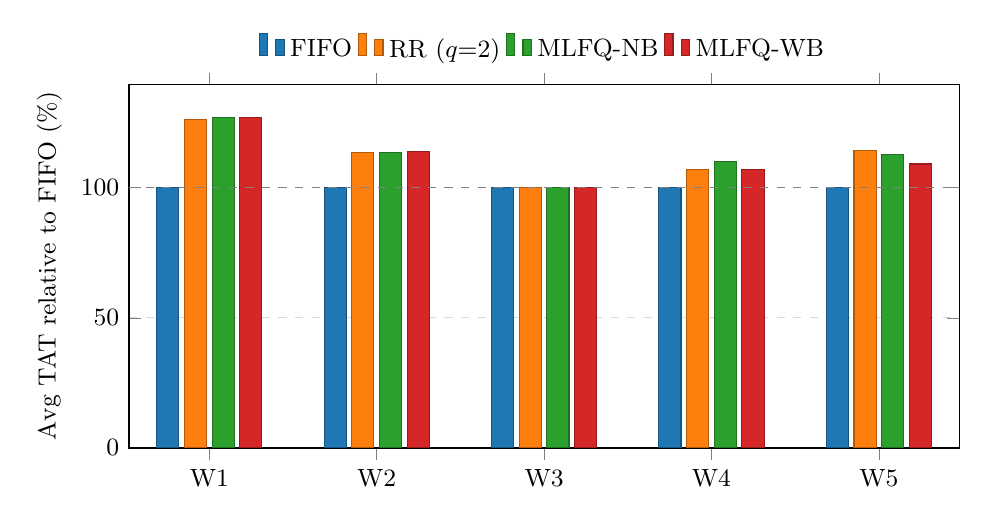
\begin{tikzpicture}
\begin{axis}[barstyle, ylabel={Avg TAT relative to FIFO (\%)}, ymin=0]
\addplot[fill=cFIFO,draw=cFIFO!70!black] coordinates {(W1,100.00) (W2,100.00) (W3,100.00) (W4,100.00) (W5,100.00)};
\addplot[fill=cRR,draw=cRR!70!black] coordinates {(W1,126.24) (W2,113.33) (W3,100.00) (W4,106.78) (W5,114.11)};
\addplot[fill=cNB,draw=cNB!70!black] coordinates {(W1,126.97) (W2,113.33) (W3,100.00) (W4,110.03) (W5,112.61)};
\addplot[fill=cWB,draw=cWB!70!black] coordinates {(W1,126.97) (W2,113.71) (W3,100.00) (W4,107.05) (W5,109.08)};
\draw[dashed,gray] ({rel axis cs:0,0}|-{axis cs:W1,100}) -- ({rel axis cs:1,0}|-{axis cs:W1,100});
\legend{FIFO, RR ($q{=}2$), MLFQ-NB, MLFQ-WB}
\end{axis}\end{tikzpicture}
\caption{Average turnaround time of each algorithm as a percentage of the FIFO result for the same workload, single processor. FIFO is the 100\,\% baseline. No preemptive policy beats FIFO on any workload; on workload 3 all four are equal.}
\end{figure}
\begin{figure}[htbp]\centering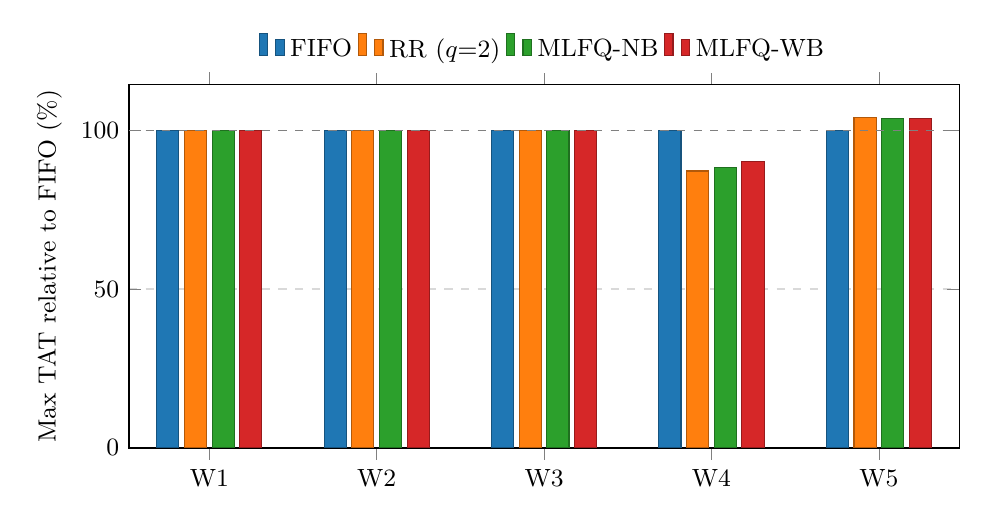
\begin{tikzpicture}
\begin{axis}[barstyle, ylabel={Max TAT relative to FIFO (\%)}, ymin=0]
\addplot[fill=cFIFO,draw=cFIFO!70!black] coordinates {(W1,100.00) (W2,100.00) (W3,100.00) (W4,100.00) (W5,100.00)};
\addplot[fill=cRR,draw=cRR!70!black] coordinates {(W1,100.00) (W2,100.00) (W3,100.00) (W4,87.12) (W5,104.00)};
\addplot[fill=cNB,draw=cNB!70!black] coordinates {(W1,100.00) (W2,100.00) (W3,100.00) (W4,88.34) (W5,103.56)};
\addplot[fill=cWB,draw=cWB!70!black] coordinates {(W1,100.00) (W2,100.00) (W3,100.00) (W4,90.18) (W5,103.56)};
\draw[dashed,gray] ({rel axis cs:0,0}|-{axis cs:W1,100}) -- ({rel axis cs:1,0}|-{axis cs:W1,100});
\legend{FIFO, RR ($q{=}2$), MLFQ-NB, MLFQ-WB}
\end{axis}\end{tikzpicture}
\caption{Maximum (worst-case) turnaround time relative to FIFO, single processor. On workload 4 every preemptive policy is clearly better than FIFO, which is where FIFO's convoy effect hurts most.}
\end{figure}
\begin{figure}[htbp]\centering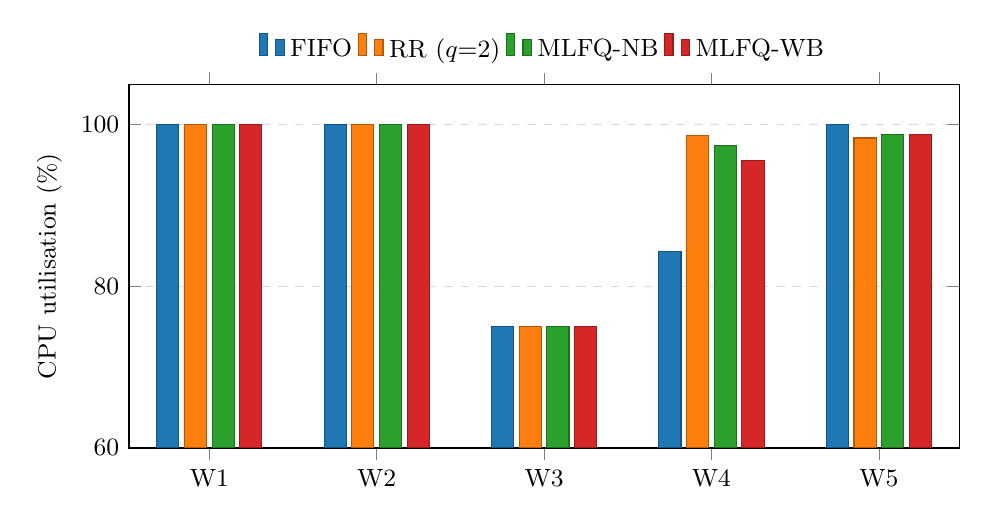
\begin{tikzpicture}
\begin{axis}[barstyle, ylabel={CPU utilisation (\%)}, ymin=60,ymax=105]
\addplot[fill=cFIFO,draw=cFIFO!70!black] coordinates {(W1,100.00) (W2,100.00) (W3,75.00) (W4,84.27) (W5,100.00)};
\addplot[fill=cRR,draw=cRR!70!black] coordinates {(W1,100.00) (W2,100.00) (W3,75.00) (W4,98.68) (W5,98.36)};
\addplot[fill=cNB,draw=cNB!70!black] coordinates {(W1,100.00) (W2,100.00) (W3,75.00) (W4,97.40) (W5,98.77)};
\addplot[fill=cWB,draw=cWB!70!black] coordinates {(W1,100.00) (W2,100.00) (W3,75.00) (W4,95.54) (W5,98.77)};
\legend{FIFO, RR ($q{=}2$), MLFQ-NB, MLFQ-WB}
\end{axis}\end{tikzpicture}
\caption{CPU utilisation, i.e.\ run time (excluding I/O) divided by total simulation time, single processor. The preemptive policies overlap I/O with computation far better on workload 4.}
\end{figure}
\begin{figure}[htbp]\centering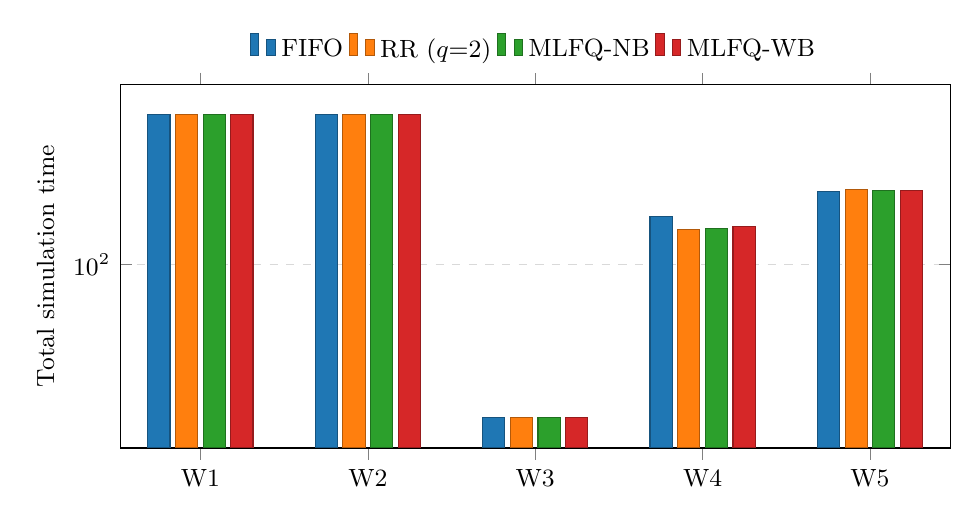
\begin{tikzpicture}
\begin{axis}[barstyle, ylabel={Total simulation time}, ymode=log,log origin=infty]
\addplot[fill=cFIFO,draw=cFIFO!70!black] coordinates {(W1,600.00) (W2,600.00) (W3,16.00) (W4,178.00) (W5,240.00)};
\addplot[fill=cRR,draw=cRR!70!black] coordinates {(W1,600.00) (W2,600.00) (W3,16.00) (W4,152.00) (W5,244.00)};
\addplot[fill=cNB,draw=cNB!70!black] coordinates {(W1,600.00) (W2,600.00) (W3,16.00) (W4,154.00) (W5,243.00)};
\addplot[fill=cWB,draw=cWB!70!black] coordinates {(W1,600.00) (W2,600.00) (W3,16.00) (W4,157.00) (W5,243.00)};
\legend{FIFO, RR ($q{=}2$), MLFQ-NB, MLFQ-WB}
\end{axis}\end{tikzpicture}
\caption{Makespan (total simulation time), single processor. Lower is better. The preemptive policies finish workload 4 substantially earlier than FIFO.}
\end{figure}
\begin{figure}[htbp]\centering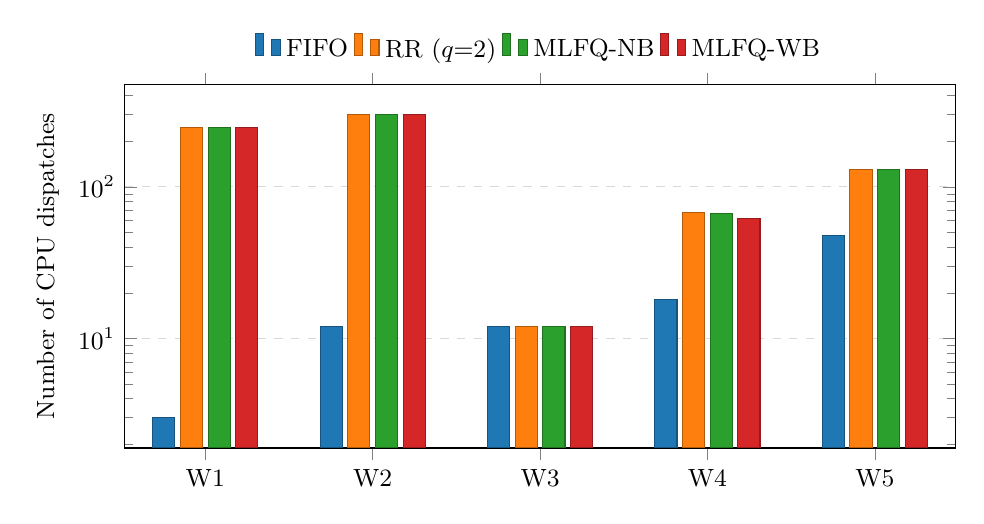
\begin{tikzpicture}
\begin{axis}[barstyle, ylabel={Number of CPU dispatches}, ymode=log,log origin=infty]
\addplot[fill=cFIFO,draw=cFIFO!70!black] coordinates {(W1,3.00) (W2,12.00) (W3,12.00) (W4,18.00) (W5,48.00)};
\addplot[fill=cRR,draw=cRR!70!black] coordinates {(W1,247.00) (W2,300.00) (W3,12.00) (W4,68.00) (W5,131.00)};
\addplot[fill=cNB,draw=cNB!70!black] coordinates {(W1,248.00) (W2,300.00) (W3,12.00) (W4,67.00) (W5,131.00)};
\addplot[fill=cWB,draw=cWB!70!black] coordinates {(W1,248.00) (W2,300.00) (W3,12.00) (W4,62.00) (W5,131.00)};
\legend{FIFO, RR ($q{=}2$), MLFQ-NB, MLFQ-WB}
\end{axis}\end{tikzpicture}
\caption{Number of contiguous CPU segments, a proxy for context-switch overhead, single processor. FIFO needs the fewest by a wide margin; this is the hidden cost of preemption.}
\end{figure}
\subsection{Per-process turnaround time}

The aggregate averages hide how differently the policies treat \emph{individual}
processes. The following five charts break the turnaround time down per process, for
every workload.

\begin{figure}[htbp]\centering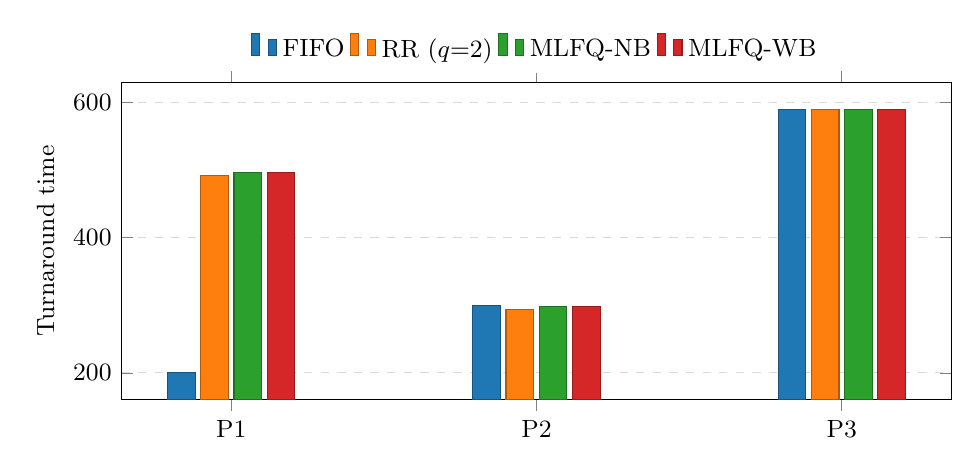
\begin{tikzpicture}
\begin{axis}[ybar,width=\textwidth,height=5.6cm,symbolic x coords={P1,P2,P3},xtick=data,
  enlarge x limits=0.18, ylabel={Turnaround time}, ymajorgrids, grid style={dashed,gray!30},
  legend style={at={(0.5,1.03)},anchor=south,legend columns=4,draw=none,font=\small},
  bar width=10pt, tick label style={font=\small}, label style={font=\small}]
\addplot[fill=cFIFO,draw=cFIFO!70!black] coordinates {(P1,200) (P2,300) (P3,590)};
\addplot[fill=cRR,draw=cRR!70!black] coordinates {(P1,492) (P2,294) (P3,590)};
\addplot[fill=cNB,draw=cNB!70!black] coordinates {(P1,496) (P2,298) (P3,590)};
\addplot[fill=cWB,draw=cWB!70!black] coordinates {(P1,496) (P2,298) (P3,590)};
\legend{FIFO, RR ($q{=}2$), MLFQ-NB, MLFQ-WB}
\end{axis}\end{tikzpicture}
\caption{Per-process turnaround time, workload 1, single processor. Three pure CPU-bound processes and no I/O at all.}
\end{figure}
\begin{figure}[htbp]\centering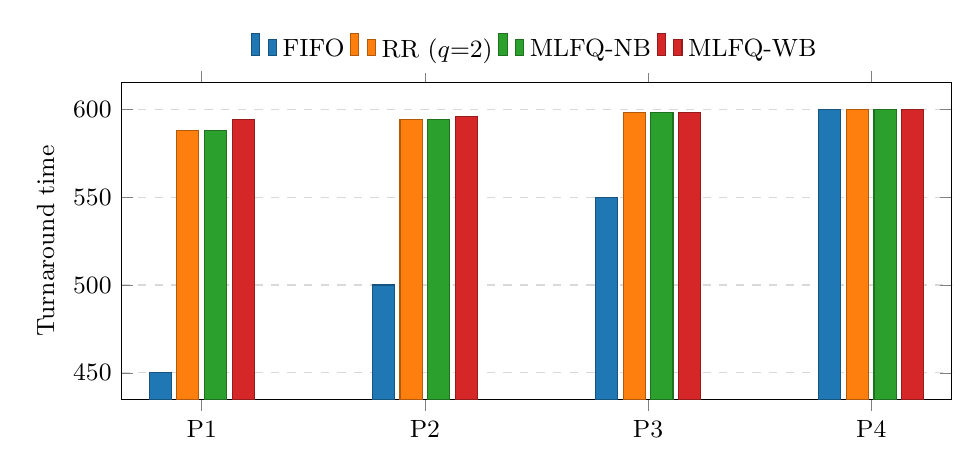
\begin{tikzpicture}
\begin{axis}[ybar,width=\textwidth,height=5.6cm,symbolic x coords={P1,P2,P3,P4},xtick=data,
  enlarge x limits=0.12, ylabel={Turnaround time}, ymajorgrids, grid style={dashed,gray!30},
  legend style={at={(0.5,1.03)},anchor=south,legend columns=4,draw=none,font=\small},
  bar width=8pt, tick label style={font=\small}, label style={font=\small}]
\addplot[fill=cFIFO,draw=cFIFO!70!black] coordinates {(P1,450) (P2,500) (P3,550) (P4,600)};
\addplot[fill=cRR,draw=cRR!70!black] coordinates {(P1,588) (P2,594) (P3,598) (P4,600)};
\addplot[fill=cNB,draw=cNB!70!black] coordinates {(P1,588) (P2,594) (P3,598) (P4,600)};
\addplot[fill=cWB,draw=cWB!70!black] coordinates {(P1,594) (P2,596) (P3,598) (P4,600)};
\legend{FIFO, RR ($q{=}2$), MLFQ-NB, MLFQ-WB}
\end{axis}\end{tikzpicture}
\caption{Per-process turnaround time, workload 2, single processor. Four identical processes with long (50-unit) CPU bursts.}
\end{figure}
\begin{figure}[htbp]\centering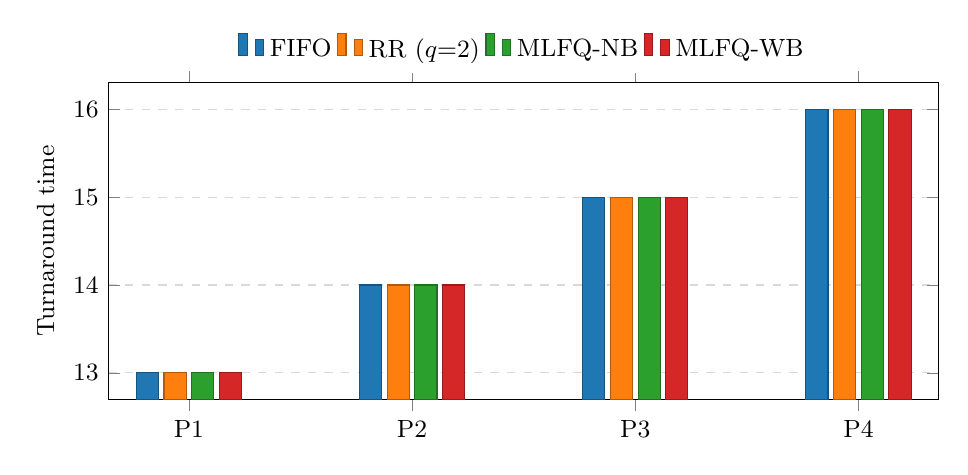
\begin{tikzpicture}
\begin{axis}[ybar,width=\textwidth,height=5.6cm,symbolic x coords={P1,P2,P3,P4},xtick=data,
  enlarge x limits=0.12, ylabel={Turnaround time}, ymajorgrids, grid style={dashed,gray!30},
  legend style={at={(0.5,1.03)},anchor=south,legend columns=4,draw=none,font=\small},
  bar width=8pt, tick label style={font=\small}, label style={font=\small}]
\addplot[fill=cFIFO,draw=cFIFO!70!black] coordinates {(P1,13) (P2,14) (P3,15) (P4,16)};
\addplot[fill=cRR,draw=cRR!70!black] coordinates {(P1,13) (P2,14) (P3,15) (P4,16)};
\addplot[fill=cNB,draw=cNB!70!black] coordinates {(P1,13) (P2,14) (P3,15) (P4,16)};
\addplot[fill=cWB,draw=cWB!70!black] coordinates {(P1,13) (P2,14) (P3,15) (P4,16)};
\legend{FIFO, RR ($q{=}2$), MLFQ-NB, MLFQ-WB}
\end{axis}\end{tikzpicture}
\caption{Per-process turnaround time, workload 3, single processor. Four identical processes whose CPU bursts are all 1 unit long.}
\end{figure}
\begin{figure}[htbp]\centering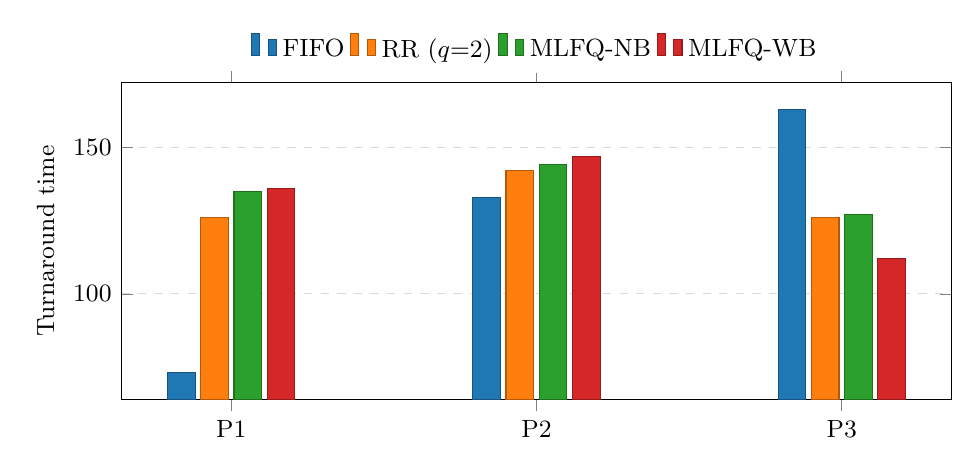
\begin{tikzpicture}
\begin{axis}[ybar,width=\textwidth,height=5.6cm,symbolic x coords={P1,P2,P3},xtick=data,
  enlarge x limits=0.18, ylabel={Turnaround time}, ymajorgrids, grid style={dashed,gray!30},
  legend style={at={(0.5,1.03)},anchor=south,legend columns=4,draw=none,font=\small},
  bar width=10pt, tick label style={font=\small}, label style={font=\small}]
\addplot[fill=cFIFO,draw=cFIFO!70!black] coordinates {(P1,73) (P2,133) (P3,163)};
\addplot[fill=cRR,draw=cRR!70!black] coordinates {(P1,126) (P2,142) (P3,126)};
\addplot[fill=cNB,draw=cNB!70!black] coordinates {(P1,135) (P2,144) (P3,127)};
\addplot[fill=cWB,draw=cWB!70!black] coordinates {(P1,136) (P2,147) (P3,112)};
\legend{FIFO, RR ($q{=}2$), MLFQ-NB, MLFQ-WB}
\end{axis}\end{tikzpicture}
\caption{Per-process turnaround time, workload 4, single processor. P1 long CPU-bound, P2 medium, P3 short interactive.}
\end{figure}
\begin{figure}[htbp]\centering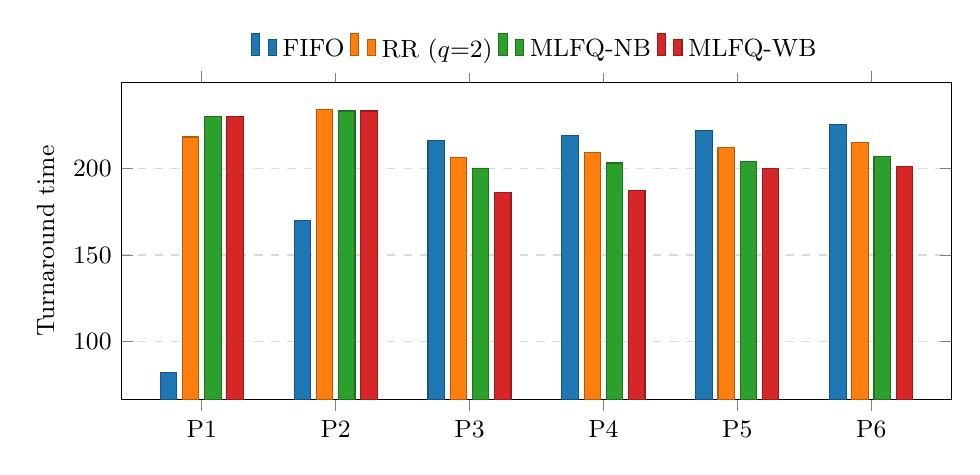
\begin{tikzpicture}
\begin{axis}[ybar,width=\textwidth,height=5.6cm,symbolic x coords={P1,P2,P3,P4,P5,P6},xtick=data,
  enlarge x limits=0.12, ylabel={Turnaround time}, ymajorgrids, grid style={dashed,gray!30},
  legend style={at={(0.5,1.03)},anchor=south,legend columns=4,draw=none,font=\small},
  bar width=6pt, tick label style={font=\small}, label style={font=\small}]
\addplot[fill=cFIFO,draw=cFIFO!70!black] coordinates {(P1,82) (P2,170) (P3,216) (P4,219) (P5,222) (P6,225)};
\addplot[fill=cRR,draw=cRR!70!black] coordinates {(P1,218) (P2,234) (P3,206) (P4,209) (P5,212) (P6,215)};
\addplot[fill=cNB,draw=cNB!70!black] coordinates {(P1,230) (P2,233) (P3,200) (P4,203) (P5,204) (P6,207)};
\addplot[fill=cWB,draw=cWB!70!black] coordinates {(P1,230) (P2,233) (P3,186) (P4,187) (P5,200) (P6,201)};
\legend{FIFO, RR ($q{=}2$), MLFQ-NB, MLFQ-WB}
\end{axis}\end{tikzpicture}
\caption{Per-process turnaround time, workload 5, single processor. P1 long, P2 medium, P3--P6 short interactive, all arriving at $t=15$.}
\end{figure}
\clearpage
\subsection{Schedule visualisation (Gantt charts)}
The clearest way to see \emph{why} the numbers differ is to look at the schedules
themselves. In the charts below each row is a process, each coloured block is a contiguous
stretch of CPU time, and white space in a row means the process is either blocked on I/O or
waiting in a ready queue. White space spanning \emph{all} rows of a chart is an idle CPU.

\begin{figure}[H]\centering
\par\vspace{1.5mm}{\small\textbf{FIFO}\quad(makespan 600, idle 0)}\par\vspace{0.8mm}
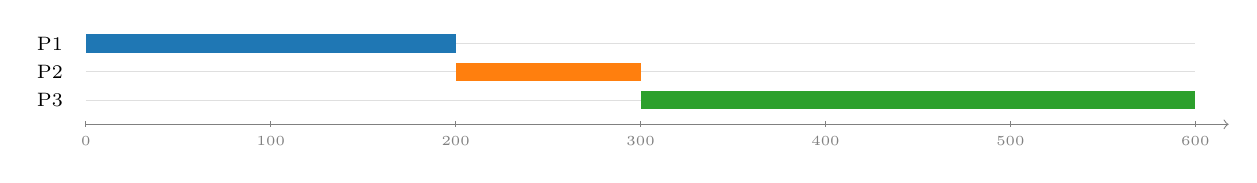
\begin{tikzpicture}[x=0.02349cm,y=0.36cm]
\node[anchor=east,font=\scriptsize] at (-7.2,2) {P1};
\draw[gray!25] (0,2) -- (600,2);
\node[anchor=east,font=\scriptsize] at (-7.2,1) {P2};
\draw[gray!25] (0,1) -- (600,1);
\node[anchor=east,font=\scriptsize] at (-7.2,0) {P3};
\draw[gray!25] (0,0) -- (600,0);
\fill[cP1] (0,1.68) rectangle (200,2.32);
\fill[cP2] (200,0.68) rectangle (300,1.32);
\fill[cP3] (300,-0.32) rectangle (600,0.32);
\draw[->,gray] (0,-0.85) -- (618.0,-0.85);
\draw[gray] (0,-0.75)--(0,-0.95) node[below,font=\tiny]{0};
\draw[gray] (100,-0.75)--(100,-0.95) node[below,font=\tiny]{100};
\draw[gray] (200,-0.75)--(200,-0.95) node[below,font=\tiny]{200};
\draw[gray] (300,-0.75)--(300,-0.95) node[below,font=\tiny]{300};
\draw[gray] (400,-0.75)--(400,-0.95) node[below,font=\tiny]{400};
\draw[gray] (500,-0.75)--(500,-0.95) node[below,font=\tiny]{500};
\draw[gray] (600,-0.75)--(600,-0.95) node[below,font=\tiny]{600};
\end{tikzpicture}\par
\par\vspace{1.5mm}{\small\textbf{RR}\quad(makespan 600, idle 0)}\par\vspace{0.8mm}
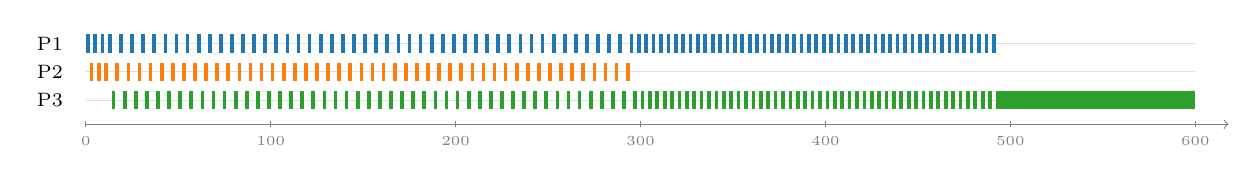
\begin{tikzpicture}[x=0.02349cm,y=0.36cm]
\node[anchor=east,font=\scriptsize] at (-7.2,2) {P1};
\draw[gray!25] (0,2) -- (600,2);
\node[anchor=east,font=\scriptsize] at (-7.2,1) {P2};
\draw[gray!25] (0,1) -- (600,1);
\node[anchor=east,font=\scriptsize] at (-7.2,0) {P3};
\draw[gray!25] (0,0) -- (600,0);
\fill[cP1] (0,1.68) rectangle (2,2.32);
\fill[cP2] (2,0.68) rectangle (4,1.32);
\fill[cP1] (4,1.68) rectangle (6,2.32);
\fill[cP2] (6,0.68) rectangle (8,1.32);
\fill[cP1] (8,1.68) rectangle (10,2.32);
\fill[cP2] (10,0.68) rectangle (12,1.32);
\fill[cP1] (12,1.68) rectangle (14,2.32);
\fill[cP3] (14,-0.32) rectangle (16,0.32);
\fill[cP2] (16,0.68) rectangle (18,1.32);
\fill[cP1] (18,1.68) rectangle (20,2.32);
\fill[cP3] (20,-0.32) rectangle (22,0.32);
\fill[cP2] (22,0.68) rectangle (24,1.32);
\fill[cP1] (24,1.68) rectangle (26,2.32);
\fill[cP3] (26,-0.32) rectangle (28,0.32);
\fill[cP2] (28,0.68) rectangle (30,1.32);
\fill[cP1] (30,1.68) rectangle (32,2.32);
\fill[cP3] (32,-0.32) rectangle (34,0.32);
\fill[cP2] (34,0.68) rectangle (36,1.32);
\fill[cP1] (36,1.68) rectangle (38,2.32);
\fill[cP3] (38,-0.32) rectangle (40,0.32);
\fill[cP2] (40,0.68) rectangle (42,1.32);
\fill[cP1] (42,1.68) rectangle (44,2.32);
\fill[cP3] (44,-0.32) rectangle (46,0.32);
\fill[cP2] (46,0.68) rectangle (48,1.32);
\fill[cP1] (48,1.68) rectangle (50,2.32);
\fill[cP3] (50,-0.32) rectangle (52,0.32);
\fill[cP2] (52,0.68) rectangle (54,1.32);
\fill[cP1] (54,1.68) rectangle (56,2.32);
\fill[cP3] (56,-0.32) rectangle (58,0.32);
\fill[cP2] (58,0.68) rectangle (60,1.32);
\fill[cP1] (60,1.68) rectangle (62,2.32);
\fill[cP3] (62,-0.32) rectangle (64,0.32);
\fill[cP2] (64,0.68) rectangle (66,1.32);
\fill[cP1] (66,1.68) rectangle (68,2.32);
\fill[cP3] (68,-0.32) rectangle (70,0.32);
\fill[cP2] (70,0.68) rectangle (72,1.32);
\fill[cP1] (72,1.68) rectangle (74,2.32);
\fill[cP3] (74,-0.32) rectangle (76,0.32);
\fill[cP2] (76,0.68) rectangle (78,1.32);
\fill[cP1] (78,1.68) rectangle (80,2.32);
\fill[cP3] (80,-0.32) rectangle (82,0.32);
\fill[cP2] (82,0.68) rectangle (84,1.32);
\fill[cP1] (84,1.68) rectangle (86,2.32);
\fill[cP3] (86,-0.32) rectangle (88,0.32);
\fill[cP2] (88,0.68) rectangle (90,1.32);
\fill[cP1] (90,1.68) rectangle (92,2.32);
\fill[cP3] (92,-0.32) rectangle (94,0.32);
\fill[cP2] (94,0.68) rectangle (96,1.32);
\fill[cP1] (96,1.68) rectangle (98,2.32);
\fill[cP3] (98,-0.32) rectangle (100,0.32);
\fill[cP2] (100,0.68) rectangle (102,1.32);
\fill[cP1] (102,1.68) rectangle (104,2.32);
\fill[cP3] (104,-0.32) rectangle (106,0.32);
\fill[cP2] (106,0.68) rectangle (108,1.32);
\fill[cP1] (108,1.68) rectangle (110,2.32);
\fill[cP3] (110,-0.32) rectangle (112,0.32);
\fill[cP2] (112,0.68) rectangle (114,1.32);
\fill[cP1] (114,1.68) rectangle (116,2.32);
\fill[cP3] (116,-0.32) rectangle (118,0.32);
\fill[cP2] (118,0.68) rectangle (120,1.32);
\fill[cP1] (120,1.68) rectangle (122,2.32);
\fill[cP3] (122,-0.32) rectangle (124,0.32);
\fill[cP2] (124,0.68) rectangle (126,1.32);
\fill[cP1] (126,1.68) rectangle (128,2.32);
\fill[cP3] (128,-0.32) rectangle (130,0.32);
\fill[cP2] (130,0.68) rectangle (132,1.32);
\fill[cP1] (132,1.68) rectangle (134,2.32);
\fill[cP3] (134,-0.32) rectangle (136,0.32);
\fill[cP2] (136,0.68) rectangle (138,1.32);
\fill[cP1] (138,1.68) rectangle (140,2.32);
\fill[cP3] (140,-0.32) rectangle (142,0.32);
\fill[cP2] (142,0.68) rectangle (144,1.32);
\fill[cP1] (144,1.68) rectangle (146,2.32);
\fill[cP3] (146,-0.32) rectangle (148,0.32);
\fill[cP2] (148,0.68) rectangle (150,1.32);
\fill[cP1] (150,1.68) rectangle (152,2.32);
\fill[cP3] (152,-0.32) rectangle (154,0.32);
\fill[cP2] (154,0.68) rectangle (156,1.32);
\fill[cP1] (156,1.68) rectangle (158,2.32);
\fill[cP3] (158,-0.32) rectangle (160,0.32);
\fill[cP2] (160,0.68) rectangle (162,1.32);
\fill[cP1] (162,1.68) rectangle (164,2.32);
\fill[cP3] (164,-0.32) rectangle (166,0.32);
\fill[cP2] (166,0.68) rectangle (168,1.32);
\fill[cP1] (168,1.68) rectangle (170,2.32);
\fill[cP3] (170,-0.32) rectangle (172,0.32);
\fill[cP2] (172,0.68) rectangle (174,1.32);
\fill[cP1] (174,1.68) rectangle (176,2.32);
\fill[cP3] (176,-0.32) rectangle (178,0.32);
\fill[cP2] (178,0.68) rectangle (180,1.32);
\fill[cP1] (180,1.68) rectangle (182,2.32);
\fill[cP3] (182,-0.32) rectangle (184,0.32);
\fill[cP2] (184,0.68) rectangle (186,1.32);
\fill[cP1] (186,1.68) rectangle (188,2.32);
\fill[cP3] (188,-0.32) rectangle (190,0.32);
\fill[cP2] (190,0.68) rectangle (192,1.32);
\fill[cP1] (192,1.68) rectangle (194,2.32);
\fill[cP3] (194,-0.32) rectangle (196,0.32);
\fill[cP2] (196,0.68) rectangle (198,1.32);
\fill[cP1] (198,1.68) rectangle (200,2.32);
\fill[cP3] (200,-0.32) rectangle (202,0.32);
\fill[cP2] (202,0.68) rectangle (204,1.32);
\fill[cP1] (204,1.68) rectangle (206,2.32);
\fill[cP3] (206,-0.32) rectangle (208,0.32);
\fill[cP2] (208,0.68) rectangle (210,1.32);
\fill[cP1] (210,1.68) rectangle (212,2.32);
\fill[cP3] (212,-0.32) rectangle (214,0.32);
\fill[cP2] (214,0.68) rectangle (216,1.32);
\fill[cP1] (216,1.68) rectangle (218,2.32);
\fill[cP3] (218,-0.32) rectangle (220,0.32);
\fill[cP2] (220,0.68) rectangle (222,1.32);
\fill[cP1] (222,1.68) rectangle (224,2.32);
\fill[cP3] (224,-0.32) rectangle (226,0.32);
\fill[cP2] (226,0.68) rectangle (228,1.32);
\fill[cP1] (228,1.68) rectangle (230,2.32);
\fill[cP3] (230,-0.32) rectangle (232,0.32);
\fill[cP2] (232,0.68) rectangle (234,1.32);
\fill[cP1] (234,1.68) rectangle (236,2.32);
\fill[cP3] (236,-0.32) rectangle (238,0.32);
\fill[cP2] (238,0.68) rectangle (240,1.32);
\fill[cP1] (240,1.68) rectangle (242,2.32);
\fill[cP3] (242,-0.32) rectangle (244,0.32);
\fill[cP2] (244,0.68) rectangle (246,1.32);
\fill[cP1] (246,1.68) rectangle (248,2.32);
\fill[cP3] (248,-0.32) rectangle (250,0.32);
\fill[cP2] (250,0.68) rectangle (252,1.32);
\fill[cP1] (252,1.68) rectangle (254,2.32);
\fill[cP3] (254,-0.32) rectangle (256,0.32);
\fill[cP2] (256,0.68) rectangle (258,1.32);
\fill[cP1] (258,1.68) rectangle (260,2.32);
\fill[cP3] (260,-0.32) rectangle (262,0.32);
\fill[cP2] (262,0.68) rectangle (264,1.32);
\fill[cP1] (264,1.68) rectangle (266,2.32);
\fill[cP3] (266,-0.32) rectangle (268,0.32);
\fill[cP2] (268,0.68) rectangle (270,1.32);
\fill[cP1] (270,1.68) rectangle (272,2.32);
\fill[cP3] (272,-0.32) rectangle (274,0.32);
\fill[cP2] (274,0.68) rectangle (276,1.32);
\fill[cP1] (276,1.68) rectangle (278,2.32);
\fill[cP3] (278,-0.32) rectangle (280,0.32);
\fill[cP2] (280,0.68) rectangle (282,1.32);
\fill[cP1] (282,1.68) rectangle (284,2.32);
\fill[cP3] (284,-0.32) rectangle (286,0.32);
\fill[cP2] (286,0.68) rectangle (288,1.32);
\fill[cP1] (288,1.68) rectangle (290,2.32);
\fill[cP3] (290,-0.32) rectangle (292,0.32);
\fill[cP2] (292,0.68) rectangle (294,1.32);
\fill[cP1] (294,1.68) rectangle (296,2.32);
\fill[cP3] (296,-0.32) rectangle (298,0.32);
\fill[cP1] (298,1.68) rectangle (300,2.32);
\fill[cP3] (300,-0.32) rectangle (302,0.32);
\fill[cP1] (302,1.68) rectangle (304,2.32);
\fill[cP3] (304,-0.32) rectangle (306,0.32);
\fill[cP1] (306,1.68) rectangle (308,2.32);
\fill[cP3] (308,-0.32) rectangle (310,0.32);
\fill[cP1] (310,1.68) rectangle (312,2.32);
\fill[cP3] (312,-0.32) rectangle (314,0.32);
\fill[cP1] (314,1.68) rectangle (316,2.32);
\fill[cP3] (316,-0.32) rectangle (318,0.32);
\fill[cP1] (318,1.68) rectangle (320,2.32);
\fill[cP3] (320,-0.32) rectangle (322,0.32);
\fill[cP1] (322,1.68) rectangle (324,2.32);
\fill[cP3] (324,-0.32) rectangle (326,0.32);
\fill[cP1] (326,1.68) rectangle (328,2.32);
\fill[cP3] (328,-0.32) rectangle (330,0.32);
\fill[cP1] (330,1.68) rectangle (332,2.32);
\fill[cP3] (332,-0.32) rectangle (334,0.32);
\fill[cP1] (334,1.68) rectangle (336,2.32);
\fill[cP3] (336,-0.32) rectangle (338,0.32);
\fill[cP1] (338,1.68) rectangle (340,2.32);
\fill[cP3] (340,-0.32) rectangle (342,0.32);
\fill[cP1] (342,1.68) rectangle (344,2.32);
\fill[cP3] (344,-0.32) rectangle (346,0.32);
\fill[cP1] (346,1.68) rectangle (348,2.32);
\fill[cP3] (348,-0.32) rectangle (350,0.32);
\fill[cP1] (350,1.68) rectangle (352,2.32);
\fill[cP3] (352,-0.32) rectangle (354,0.32);
\fill[cP1] (354,1.68) rectangle (356,2.32);
\fill[cP3] (356,-0.32) rectangle (358,0.32);
\fill[cP1] (358,1.68) rectangle (360,2.32);
\fill[cP3] (360,-0.32) rectangle (362,0.32);
\fill[cP1] (362,1.68) rectangle (364,2.32);
\fill[cP3] (364,-0.32) rectangle (366,0.32);
\fill[cP1] (366,1.68) rectangle (368,2.32);
\fill[cP3] (368,-0.32) rectangle (370,0.32);
\fill[cP1] (370,1.68) rectangle (372,2.32);
\fill[cP3] (372,-0.32) rectangle (374,0.32);
\fill[cP1] (374,1.68) rectangle (376,2.32);
\fill[cP3] (376,-0.32) rectangle (378,0.32);
\fill[cP1] (378,1.68) rectangle (380,2.32);
\fill[cP3] (380,-0.32) rectangle (382,0.32);
\fill[cP1] (382,1.68) rectangle (384,2.32);
\fill[cP3] (384,-0.32) rectangle (386,0.32);
\fill[cP1] (386,1.68) rectangle (388,2.32);
\fill[cP3] (388,-0.32) rectangle (390,0.32);
\fill[cP1] (390,1.68) rectangle (392,2.32);
\fill[cP3] (392,-0.32) rectangle (394,0.32);
\fill[cP1] (394,1.68) rectangle (396,2.32);
\fill[cP3] (396,-0.32) rectangle (398,0.32);
\fill[cP1] (398,1.68) rectangle (400,2.32);
\fill[cP3] (400,-0.32) rectangle (402,0.32);
\fill[cP1] (402,1.68) rectangle (404,2.32);
\fill[cP3] (404,-0.32) rectangle (406,0.32);
\fill[cP1] (406,1.68) rectangle (408,2.32);
\fill[cP3] (408,-0.32) rectangle (410,0.32);
\fill[cP1] (410,1.68) rectangle (412,2.32);
\fill[cP3] (412,-0.32) rectangle (414,0.32);
\fill[cP1] (414,1.68) rectangle (416,2.32);
\fill[cP3] (416,-0.32) rectangle (418,0.32);
\fill[cP1] (418,1.68) rectangle (420,2.32);
\fill[cP3] (420,-0.32) rectangle (422,0.32);
\fill[cP1] (422,1.68) rectangle (424,2.32);
\fill[cP3] (424,-0.32) rectangle (426,0.32);
\fill[cP1] (426,1.68) rectangle (428,2.32);
\fill[cP3] (428,-0.32) rectangle (430,0.32);
\fill[cP1] (430,1.68) rectangle (432,2.32);
\fill[cP3] (432,-0.32) rectangle (434,0.32);
\fill[cP1] (434,1.68) rectangle (436,2.32);
\fill[cP3] (436,-0.32) rectangle (438,0.32);
\fill[cP1] (438,1.68) rectangle (440,2.32);
\fill[cP3] (440,-0.32) rectangle (442,0.32);
\fill[cP1] (442,1.68) rectangle (444,2.32);
\fill[cP3] (444,-0.32) rectangle (446,0.32);
\fill[cP1] (446,1.68) rectangle (448,2.32);
\fill[cP3] (448,-0.32) rectangle (450,0.32);
\fill[cP1] (450,1.68) rectangle (452,2.32);
\fill[cP3] (452,-0.32) rectangle (454,0.32);
\fill[cP1] (454,1.68) rectangle (456,2.32);
\fill[cP3] (456,-0.32) rectangle (458,0.32);
\fill[cP1] (458,1.68) rectangle (460,2.32);
\fill[cP3] (460,-0.32) rectangle (462,0.32);
\fill[cP1] (462,1.68) rectangle (464,2.32);
\fill[cP3] (464,-0.32) rectangle (466,0.32);
\fill[cP1] (466,1.68) rectangle (468,2.32);
\fill[cP3] (468,-0.32) rectangle (470,0.32);
\fill[cP1] (470,1.68) rectangle (472,2.32);
\fill[cP3] (472,-0.32) rectangle (474,0.32);
\fill[cP1] (474,1.68) rectangle (476,2.32);
\fill[cP3] (476,-0.32) rectangle (478,0.32);
\fill[cP1] (478,1.68) rectangle (480,2.32);
\fill[cP3] (480,-0.32) rectangle (482,0.32);
\fill[cP1] (482,1.68) rectangle (484,2.32);
\fill[cP3] (484,-0.32) rectangle (486,0.32);
\fill[cP1] (486,1.68) rectangle (488,2.32);
\fill[cP3] (488,-0.32) rectangle (490,0.32);
\fill[cP1] (490,1.68) rectangle (492,2.32);
\fill[cP3] (492,-0.32) rectangle (600,0.32);
\draw[->,gray] (0,-0.85) -- (618.0,-0.85);
\draw[gray] (0,-0.75)--(0,-0.95) node[below,font=\tiny]{0};
\draw[gray] (100,-0.75)--(100,-0.95) node[below,font=\tiny]{100};
\draw[gray] (200,-0.75)--(200,-0.95) node[below,font=\tiny]{200};
\draw[gray] (300,-0.75)--(300,-0.95) node[below,font=\tiny]{300};
\draw[gray] (400,-0.75)--(400,-0.95) node[below,font=\tiny]{400};
\draw[gray] (500,-0.75)--(500,-0.95) node[below,font=\tiny]{500};
\draw[gray] (600,-0.75)--(600,-0.95) node[below,font=\tiny]{600};
\end{tikzpicture}\par
\par\vspace{1.5mm}{\small\textbf{MLFQ-NB}\quad(makespan 600, idle 0)}\par\vspace{0.8mm}
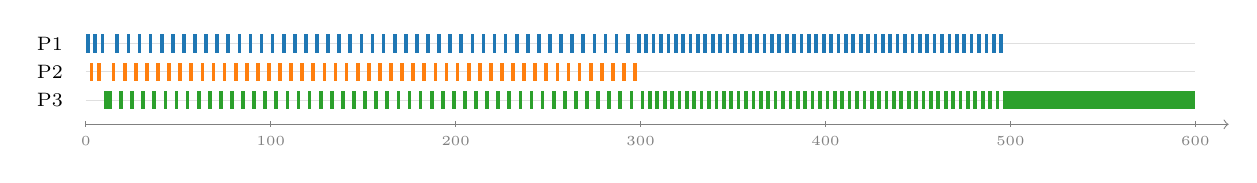
\begin{tikzpicture}[x=0.02349cm,y=0.36cm]
\node[anchor=east,font=\scriptsize] at (-7.2,2) {P1};
\draw[gray!25] (0,2) -- (600,2);
\node[anchor=east,font=\scriptsize] at (-7.2,1) {P2};
\draw[gray!25] (0,1) -- (600,1);
\node[anchor=east,font=\scriptsize] at (-7.2,0) {P3};
\draw[gray!25] (0,0) -- (600,0);
\fill[cP1] (0,1.68) rectangle (2,2.32);
\fill[cP2] (2,0.68) rectangle (4,1.32);
\fill[cP1] (4,1.68) rectangle (6,2.32);
\fill[cP2] (6,0.68) rectangle (8,1.32);
\fill[cP1] (8,1.68) rectangle (10,2.32);
\fill[cP3] (10,-0.32) rectangle (14,0.32);
\fill[cP2] (14,0.68) rectangle (16,1.32);
\fill[cP1] (16,1.68) rectangle (18,2.32);
\fill[cP3] (18,-0.32) rectangle (20,0.32);
\fill[cP2] (20,0.68) rectangle (22,1.32);
\fill[cP1] (22,1.68) rectangle (24,2.32);
\fill[cP3] (24,-0.32) rectangle (26,0.32);
\fill[cP2] (26,0.68) rectangle (28,1.32);
\fill[cP1] (28,1.68) rectangle (30,2.32);
\fill[cP3] (30,-0.32) rectangle (32,0.32);
\fill[cP2] (32,0.68) rectangle (34,1.32);
\fill[cP1] (34,1.68) rectangle (36,2.32);
\fill[cP3] (36,-0.32) rectangle (38,0.32);
\fill[cP2] (38,0.68) rectangle (40,1.32);
\fill[cP1] (40,1.68) rectangle (42,2.32);
\fill[cP3] (42,-0.32) rectangle (44,0.32);
\fill[cP2] (44,0.68) rectangle (46,1.32);
\fill[cP1] (46,1.68) rectangle (48,2.32);
\fill[cP3] (48,-0.32) rectangle (50,0.32);
\fill[cP2] (50,0.68) rectangle (52,1.32);
\fill[cP1] (52,1.68) rectangle (54,2.32);
\fill[cP3] (54,-0.32) rectangle (56,0.32);
\fill[cP2] (56,0.68) rectangle (58,1.32);
\fill[cP1] (58,1.68) rectangle (60,2.32);
\fill[cP3] (60,-0.32) rectangle (62,0.32);
\fill[cP2] (62,0.68) rectangle (64,1.32);
\fill[cP1] (64,1.68) rectangle (66,2.32);
\fill[cP3] (66,-0.32) rectangle (68,0.32);
\fill[cP2] (68,0.68) rectangle (70,1.32);
\fill[cP1] (70,1.68) rectangle (72,2.32);
\fill[cP3] (72,-0.32) rectangle (74,0.32);
\fill[cP2] (74,0.68) rectangle (76,1.32);
\fill[cP1] (76,1.68) rectangle (78,2.32);
\fill[cP3] (78,-0.32) rectangle (80,0.32);
\fill[cP2] (80,0.68) rectangle (82,1.32);
\fill[cP1] (82,1.68) rectangle (84,2.32);
\fill[cP3] (84,-0.32) rectangle (86,0.32);
\fill[cP2] (86,0.68) rectangle (88,1.32);
\fill[cP1] (88,1.68) rectangle (90,2.32);
\fill[cP3] (90,-0.32) rectangle (92,0.32);
\fill[cP2] (92,0.68) rectangle (94,1.32);
\fill[cP1] (94,1.68) rectangle (96,2.32);
\fill[cP3] (96,-0.32) rectangle (98,0.32);
\fill[cP2] (98,0.68) rectangle (100,1.32);
\fill[cP1] (100,1.68) rectangle (102,2.32);
\fill[cP3] (102,-0.32) rectangle (104,0.32);
\fill[cP2] (104,0.68) rectangle (106,1.32);
\fill[cP1] (106,1.68) rectangle (108,2.32);
\fill[cP3] (108,-0.32) rectangle (110,0.32);
\fill[cP2] (110,0.68) rectangle (112,1.32);
\fill[cP1] (112,1.68) rectangle (114,2.32);
\fill[cP3] (114,-0.32) rectangle (116,0.32);
\fill[cP2] (116,0.68) rectangle (118,1.32);
\fill[cP1] (118,1.68) rectangle (120,2.32);
\fill[cP3] (120,-0.32) rectangle (122,0.32);
\fill[cP2] (122,0.68) rectangle (124,1.32);
\fill[cP1] (124,1.68) rectangle (126,2.32);
\fill[cP3] (126,-0.32) rectangle (128,0.32);
\fill[cP2] (128,0.68) rectangle (130,1.32);
\fill[cP1] (130,1.68) rectangle (132,2.32);
\fill[cP3] (132,-0.32) rectangle (134,0.32);
\fill[cP2] (134,0.68) rectangle (136,1.32);
\fill[cP1] (136,1.68) rectangle (138,2.32);
\fill[cP3] (138,-0.32) rectangle (140,0.32);
\fill[cP2] (140,0.68) rectangle (142,1.32);
\fill[cP1] (142,1.68) rectangle (144,2.32);
\fill[cP3] (144,-0.32) rectangle (146,0.32);
\fill[cP2] (146,0.68) rectangle (148,1.32);
\fill[cP1] (148,1.68) rectangle (150,2.32);
\fill[cP3] (150,-0.32) rectangle (152,0.32);
\fill[cP2] (152,0.68) rectangle (154,1.32);
\fill[cP1] (154,1.68) rectangle (156,2.32);
\fill[cP3] (156,-0.32) rectangle (158,0.32);
\fill[cP2] (158,0.68) rectangle (160,1.32);
\fill[cP1] (160,1.68) rectangle (162,2.32);
\fill[cP3] (162,-0.32) rectangle (164,0.32);
\fill[cP2] (164,0.68) rectangle (166,1.32);
\fill[cP1] (166,1.68) rectangle (168,2.32);
\fill[cP3] (168,-0.32) rectangle (170,0.32);
\fill[cP2] (170,0.68) rectangle (172,1.32);
\fill[cP1] (172,1.68) rectangle (174,2.32);
\fill[cP3] (174,-0.32) rectangle (176,0.32);
\fill[cP2] (176,0.68) rectangle (178,1.32);
\fill[cP1] (178,1.68) rectangle (180,2.32);
\fill[cP3] (180,-0.32) rectangle (182,0.32);
\fill[cP2] (182,0.68) rectangle (184,1.32);
\fill[cP1] (184,1.68) rectangle (186,2.32);
\fill[cP3] (186,-0.32) rectangle (188,0.32);
\fill[cP2] (188,0.68) rectangle (190,1.32);
\fill[cP1] (190,1.68) rectangle (192,2.32);
\fill[cP3] (192,-0.32) rectangle (194,0.32);
\fill[cP2] (194,0.68) rectangle (196,1.32);
\fill[cP1] (196,1.68) rectangle (198,2.32);
\fill[cP3] (198,-0.32) rectangle (200,0.32);
\fill[cP2] (200,0.68) rectangle (202,1.32);
\fill[cP1] (202,1.68) rectangle (204,2.32);
\fill[cP3] (204,-0.32) rectangle (206,0.32);
\fill[cP2] (206,0.68) rectangle (208,1.32);
\fill[cP1] (208,1.68) rectangle (210,2.32);
\fill[cP3] (210,-0.32) rectangle (212,0.32);
\fill[cP2] (212,0.68) rectangle (214,1.32);
\fill[cP1] (214,1.68) rectangle (216,2.32);
\fill[cP3] (216,-0.32) rectangle (218,0.32);
\fill[cP2] (218,0.68) rectangle (220,1.32);
\fill[cP1] (220,1.68) rectangle (222,2.32);
\fill[cP3] (222,-0.32) rectangle (224,0.32);
\fill[cP2] (224,0.68) rectangle (226,1.32);
\fill[cP1] (226,1.68) rectangle (228,2.32);
\fill[cP3] (228,-0.32) rectangle (230,0.32);
\fill[cP2] (230,0.68) rectangle (232,1.32);
\fill[cP1] (232,1.68) rectangle (234,2.32);
\fill[cP3] (234,-0.32) rectangle (236,0.32);
\fill[cP2] (236,0.68) rectangle (238,1.32);
\fill[cP1] (238,1.68) rectangle (240,2.32);
\fill[cP3] (240,-0.32) rectangle (242,0.32);
\fill[cP2] (242,0.68) rectangle (244,1.32);
\fill[cP1] (244,1.68) rectangle (246,2.32);
\fill[cP3] (246,-0.32) rectangle (248,0.32);
\fill[cP2] (248,0.68) rectangle (250,1.32);
\fill[cP1] (250,1.68) rectangle (252,2.32);
\fill[cP3] (252,-0.32) rectangle (254,0.32);
\fill[cP2] (254,0.68) rectangle (256,1.32);
\fill[cP1] (256,1.68) rectangle (258,2.32);
\fill[cP3] (258,-0.32) rectangle (260,0.32);
\fill[cP2] (260,0.68) rectangle (262,1.32);
\fill[cP1] (262,1.68) rectangle (264,2.32);
\fill[cP3] (264,-0.32) rectangle (266,0.32);
\fill[cP2] (266,0.68) rectangle (268,1.32);
\fill[cP1] (268,1.68) rectangle (270,2.32);
\fill[cP3] (270,-0.32) rectangle (272,0.32);
\fill[cP2] (272,0.68) rectangle (274,1.32);
\fill[cP1] (274,1.68) rectangle (276,2.32);
\fill[cP3] (276,-0.32) rectangle (278,0.32);
\fill[cP2] (278,0.68) rectangle (280,1.32);
\fill[cP1] (280,1.68) rectangle (282,2.32);
\fill[cP3] (282,-0.32) rectangle (284,0.32);
\fill[cP2] (284,0.68) rectangle (286,1.32);
\fill[cP1] (286,1.68) rectangle (288,2.32);
\fill[cP3] (288,-0.32) rectangle (290,0.32);
\fill[cP2] (290,0.68) rectangle (292,1.32);
\fill[cP1] (292,1.68) rectangle (294,2.32);
\fill[cP3] (294,-0.32) rectangle (296,0.32);
\fill[cP2] (296,0.68) rectangle (298,1.32);
\fill[cP1] (298,1.68) rectangle (300,2.32);
\fill[cP3] (300,-0.32) rectangle (302,0.32);
\fill[cP1] (302,1.68) rectangle (304,2.32);
\fill[cP3] (304,-0.32) rectangle (306,0.32);
\fill[cP1] (306,1.68) rectangle (308,2.32);
\fill[cP3] (308,-0.32) rectangle (310,0.32);
\fill[cP1] (310,1.68) rectangle (312,2.32);
\fill[cP3] (312,-0.32) rectangle (314,0.32);
\fill[cP1] (314,1.68) rectangle (316,2.32);
\fill[cP3] (316,-0.32) rectangle (318,0.32);
\fill[cP1] (318,1.68) rectangle (320,2.32);
\fill[cP3] (320,-0.32) rectangle (322,0.32);
\fill[cP1] (322,1.68) rectangle (324,2.32);
\fill[cP3] (324,-0.32) rectangle (326,0.32);
\fill[cP1] (326,1.68) rectangle (328,2.32);
\fill[cP3] (328,-0.32) rectangle (330,0.32);
\fill[cP1] (330,1.68) rectangle (332,2.32);
\fill[cP3] (332,-0.32) rectangle (334,0.32);
\fill[cP1] (334,1.68) rectangle (336,2.32);
\fill[cP3] (336,-0.32) rectangle (338,0.32);
\fill[cP1] (338,1.68) rectangle (340,2.32);
\fill[cP3] (340,-0.32) rectangle (342,0.32);
\fill[cP1] (342,1.68) rectangle (344,2.32);
\fill[cP3] (344,-0.32) rectangle (346,0.32);
\fill[cP1] (346,1.68) rectangle (348,2.32);
\fill[cP3] (348,-0.32) rectangle (350,0.32);
\fill[cP1] (350,1.68) rectangle (352,2.32);
\fill[cP3] (352,-0.32) rectangle (354,0.32);
\fill[cP1] (354,1.68) rectangle (356,2.32);
\fill[cP3] (356,-0.32) rectangle (358,0.32);
\fill[cP1] (358,1.68) rectangle (360,2.32);
\fill[cP3] (360,-0.32) rectangle (362,0.32);
\fill[cP1] (362,1.68) rectangle (364,2.32);
\fill[cP3] (364,-0.32) rectangle (366,0.32);
\fill[cP1] (366,1.68) rectangle (368,2.32);
\fill[cP3] (368,-0.32) rectangle (370,0.32);
\fill[cP1] (370,1.68) rectangle (372,2.32);
\fill[cP3] (372,-0.32) rectangle (374,0.32);
\fill[cP1] (374,1.68) rectangle (376,2.32);
\fill[cP3] (376,-0.32) rectangle (378,0.32);
\fill[cP1] (378,1.68) rectangle (380,2.32);
\fill[cP3] (380,-0.32) rectangle (382,0.32);
\fill[cP1] (382,1.68) rectangle (384,2.32);
\fill[cP3] (384,-0.32) rectangle (386,0.32);
\fill[cP1] (386,1.68) rectangle (388,2.32);
\fill[cP3] (388,-0.32) rectangle (390,0.32);
\fill[cP1] (390,1.68) rectangle (392,2.32);
\fill[cP3] (392,-0.32) rectangle (394,0.32);
\fill[cP1] (394,1.68) rectangle (396,2.32);
\fill[cP3] (396,-0.32) rectangle (398,0.32);
\fill[cP1] (398,1.68) rectangle (400,2.32);
\fill[cP3] (400,-0.32) rectangle (402,0.32);
\fill[cP1] (402,1.68) rectangle (404,2.32);
\fill[cP3] (404,-0.32) rectangle (406,0.32);
\fill[cP1] (406,1.68) rectangle (408,2.32);
\fill[cP3] (408,-0.32) rectangle (410,0.32);
\fill[cP1] (410,1.68) rectangle (412,2.32);
\fill[cP3] (412,-0.32) rectangle (414,0.32);
\fill[cP1] (414,1.68) rectangle (416,2.32);
\fill[cP3] (416,-0.32) rectangle (418,0.32);
\fill[cP1] (418,1.68) rectangle (420,2.32);
\fill[cP3] (420,-0.32) rectangle (422,0.32);
\fill[cP1] (422,1.68) rectangle (424,2.32);
\fill[cP3] (424,-0.32) rectangle (426,0.32);
\fill[cP1] (426,1.68) rectangle (428,2.32);
\fill[cP3] (428,-0.32) rectangle (430,0.32);
\fill[cP1] (430,1.68) rectangle (432,2.32);
\fill[cP3] (432,-0.32) rectangle (434,0.32);
\fill[cP1] (434,1.68) rectangle (436,2.32);
\fill[cP3] (436,-0.32) rectangle (438,0.32);
\fill[cP1] (438,1.68) rectangle (440,2.32);
\fill[cP3] (440,-0.32) rectangle (442,0.32);
\fill[cP1] (442,1.68) rectangle (444,2.32);
\fill[cP3] (444,-0.32) rectangle (446,0.32);
\fill[cP1] (446,1.68) rectangle (448,2.32);
\fill[cP3] (448,-0.32) rectangle (450,0.32);
\fill[cP1] (450,1.68) rectangle (452,2.32);
\fill[cP3] (452,-0.32) rectangle (454,0.32);
\fill[cP1] (454,1.68) rectangle (456,2.32);
\fill[cP3] (456,-0.32) rectangle (458,0.32);
\fill[cP1] (458,1.68) rectangle (460,2.32);
\fill[cP3] (460,-0.32) rectangle (462,0.32);
\fill[cP1] (462,1.68) rectangle (464,2.32);
\fill[cP3] (464,-0.32) rectangle (466,0.32);
\fill[cP1] (466,1.68) rectangle (468,2.32);
\fill[cP3] (468,-0.32) rectangle (470,0.32);
\fill[cP1] (470,1.68) rectangle (472,2.32);
\fill[cP3] (472,-0.32) rectangle (474,0.32);
\fill[cP1] (474,1.68) rectangle (476,2.32);
\fill[cP3] (476,-0.32) rectangle (478,0.32);
\fill[cP1] (478,1.68) rectangle (480,2.32);
\fill[cP3] (480,-0.32) rectangle (482,0.32);
\fill[cP1] (482,1.68) rectangle (484,2.32);
\fill[cP3] (484,-0.32) rectangle (486,0.32);
\fill[cP1] (486,1.68) rectangle (488,2.32);
\fill[cP3] (488,-0.32) rectangle (490,0.32);
\fill[cP1] (490,1.68) rectangle (492,2.32);
\fill[cP3] (492,-0.32) rectangle (494,0.32);
\fill[cP1] (494,1.68) rectangle (496,2.32);
\fill[cP3] (496,-0.32) rectangle (600,0.32);
\draw[->,gray] (0,-0.85) -- (618.0,-0.85);
\draw[gray] (0,-0.75)--(0,-0.95) node[below,font=\tiny]{0};
\draw[gray] (100,-0.75)--(100,-0.95) node[below,font=\tiny]{100};
\draw[gray] (200,-0.75)--(200,-0.95) node[below,font=\tiny]{200};
\draw[gray] (300,-0.75)--(300,-0.95) node[below,font=\tiny]{300};
\draw[gray] (400,-0.75)--(400,-0.95) node[below,font=\tiny]{400};
\draw[gray] (500,-0.75)--(500,-0.95) node[below,font=\tiny]{500};
\draw[gray] (600,-0.75)--(600,-0.95) node[below,font=\tiny]{600};
\end{tikzpicture}\par
\par\vspace{1.5mm}{\small\textbf{MLFQ-WB}\quad(makespan 600, idle 0)}\par\vspace{0.8mm}
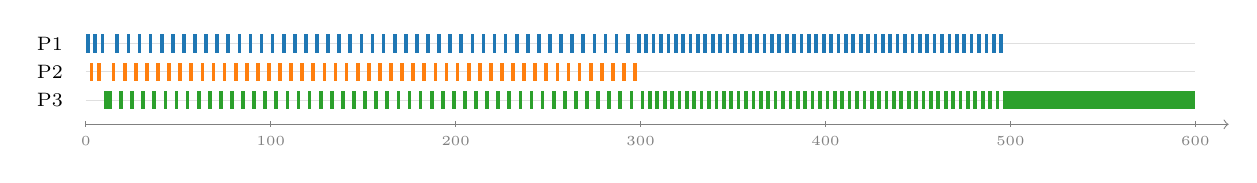
\begin{tikzpicture}[x=0.02349cm,y=0.36cm]
\node[anchor=east,font=\scriptsize] at (-7.2,2) {P1};
\draw[gray!25] (0,2) -- (600,2);
\node[anchor=east,font=\scriptsize] at (-7.2,1) {P2};
\draw[gray!25] (0,1) -- (600,1);
\node[anchor=east,font=\scriptsize] at (-7.2,0) {P3};
\draw[gray!25] (0,0) -- (600,0);
\fill[cP1] (0,1.68) rectangle (2,2.32);
\fill[cP2] (2,0.68) rectangle (4,1.32);
\fill[cP1] (4,1.68) rectangle (6,2.32);
\fill[cP2] (6,0.68) rectangle (8,1.32);
\fill[cP1] (8,1.68) rectangle (10,2.32);
\fill[cP3] (10,-0.32) rectangle (14,0.32);
\fill[cP2] (14,0.68) rectangle (16,1.32);
\fill[cP1] (16,1.68) rectangle (18,2.32);
\fill[cP3] (18,-0.32) rectangle (20,0.32);
\fill[cP2] (20,0.68) rectangle (22,1.32);
\fill[cP1] (22,1.68) rectangle (24,2.32);
\fill[cP3] (24,-0.32) rectangle (26,0.32);
\fill[cP2] (26,0.68) rectangle (28,1.32);
\fill[cP1] (28,1.68) rectangle (30,2.32);
\fill[cP3] (30,-0.32) rectangle (32,0.32);
\fill[cP2] (32,0.68) rectangle (34,1.32);
\fill[cP1] (34,1.68) rectangle (36,2.32);
\fill[cP3] (36,-0.32) rectangle (38,0.32);
\fill[cP2] (38,0.68) rectangle (40,1.32);
\fill[cP1] (40,1.68) rectangle (42,2.32);
\fill[cP3] (42,-0.32) rectangle (44,0.32);
\fill[cP2] (44,0.68) rectangle (46,1.32);
\fill[cP1] (46,1.68) rectangle (48,2.32);
\fill[cP3] (48,-0.32) rectangle (50,0.32);
\fill[cP2] (50,0.68) rectangle (52,1.32);
\fill[cP1] (52,1.68) rectangle (54,2.32);
\fill[cP3] (54,-0.32) rectangle (56,0.32);
\fill[cP2] (56,0.68) rectangle (58,1.32);
\fill[cP1] (58,1.68) rectangle (60,2.32);
\fill[cP3] (60,-0.32) rectangle (62,0.32);
\fill[cP2] (62,0.68) rectangle (64,1.32);
\fill[cP1] (64,1.68) rectangle (66,2.32);
\fill[cP3] (66,-0.32) rectangle (68,0.32);
\fill[cP2] (68,0.68) rectangle (70,1.32);
\fill[cP1] (70,1.68) rectangle (72,2.32);
\fill[cP3] (72,-0.32) rectangle (74,0.32);
\fill[cP2] (74,0.68) rectangle (76,1.32);
\fill[cP1] (76,1.68) rectangle (78,2.32);
\fill[cP3] (78,-0.32) rectangle (80,0.32);
\fill[cP2] (80,0.68) rectangle (82,1.32);
\fill[cP1] (82,1.68) rectangle (84,2.32);
\fill[cP3] (84,-0.32) rectangle (86,0.32);
\fill[cP2] (86,0.68) rectangle (88,1.32);
\fill[cP1] (88,1.68) rectangle (90,2.32);
\fill[cP3] (90,-0.32) rectangle (92,0.32);
\fill[cP2] (92,0.68) rectangle (94,1.32);
\fill[cP1] (94,1.68) rectangle (96,2.32);
\fill[cP3] (96,-0.32) rectangle (98,0.32);
\fill[cP2] (98,0.68) rectangle (100,1.32);
\fill[cP1] (100,1.68) rectangle (102,2.32);
\fill[cP3] (102,-0.32) rectangle (104,0.32);
\fill[cP2] (104,0.68) rectangle (106,1.32);
\fill[cP1] (106,1.68) rectangle (108,2.32);
\fill[cP3] (108,-0.32) rectangle (110,0.32);
\fill[cP2] (110,0.68) rectangle (112,1.32);
\fill[cP1] (112,1.68) rectangle (114,2.32);
\fill[cP3] (114,-0.32) rectangle (116,0.32);
\fill[cP2] (116,0.68) rectangle (118,1.32);
\fill[cP1] (118,1.68) rectangle (120,2.32);
\fill[cP3] (120,-0.32) rectangle (122,0.32);
\fill[cP2] (122,0.68) rectangle (124,1.32);
\fill[cP1] (124,1.68) rectangle (126,2.32);
\fill[cP3] (126,-0.32) rectangle (128,0.32);
\fill[cP2] (128,0.68) rectangle (130,1.32);
\fill[cP1] (130,1.68) rectangle (132,2.32);
\fill[cP3] (132,-0.32) rectangle (134,0.32);
\fill[cP2] (134,0.68) rectangle (136,1.32);
\fill[cP1] (136,1.68) rectangle (138,2.32);
\fill[cP3] (138,-0.32) rectangle (140,0.32);
\fill[cP2] (140,0.68) rectangle (142,1.32);
\fill[cP1] (142,1.68) rectangle (144,2.32);
\fill[cP3] (144,-0.32) rectangle (146,0.32);
\fill[cP2] (146,0.68) rectangle (148,1.32);
\fill[cP1] (148,1.68) rectangle (150,2.32);
\fill[cP3] (150,-0.32) rectangle (152,0.32);
\fill[cP2] (152,0.68) rectangle (154,1.32);
\fill[cP1] (154,1.68) rectangle (156,2.32);
\fill[cP3] (156,-0.32) rectangle (158,0.32);
\fill[cP2] (158,0.68) rectangle (160,1.32);
\fill[cP1] (160,1.68) rectangle (162,2.32);
\fill[cP3] (162,-0.32) rectangle (164,0.32);
\fill[cP2] (164,0.68) rectangle (166,1.32);
\fill[cP1] (166,1.68) rectangle (168,2.32);
\fill[cP3] (168,-0.32) rectangle (170,0.32);
\fill[cP2] (170,0.68) rectangle (172,1.32);
\fill[cP1] (172,1.68) rectangle (174,2.32);
\fill[cP3] (174,-0.32) rectangle (176,0.32);
\fill[cP2] (176,0.68) rectangle (178,1.32);
\fill[cP1] (178,1.68) rectangle (180,2.32);
\fill[cP3] (180,-0.32) rectangle (182,0.32);
\fill[cP2] (182,0.68) rectangle (184,1.32);
\fill[cP1] (184,1.68) rectangle (186,2.32);
\fill[cP3] (186,-0.32) rectangle (188,0.32);
\fill[cP2] (188,0.68) rectangle (190,1.32);
\fill[cP1] (190,1.68) rectangle (192,2.32);
\fill[cP3] (192,-0.32) rectangle (194,0.32);
\fill[cP2] (194,0.68) rectangle (196,1.32);
\fill[cP1] (196,1.68) rectangle (198,2.32);
\fill[cP3] (198,-0.32) rectangle (200,0.32);
\fill[cP2] (200,0.68) rectangle (202,1.32);
\fill[cP1] (202,1.68) rectangle (204,2.32);
\fill[cP3] (204,-0.32) rectangle (206,0.32);
\fill[cP2] (206,0.68) rectangle (208,1.32);
\fill[cP1] (208,1.68) rectangle (210,2.32);
\fill[cP3] (210,-0.32) rectangle (212,0.32);
\fill[cP2] (212,0.68) rectangle (214,1.32);
\fill[cP1] (214,1.68) rectangle (216,2.32);
\fill[cP3] (216,-0.32) rectangle (218,0.32);
\fill[cP2] (218,0.68) rectangle (220,1.32);
\fill[cP1] (220,1.68) rectangle (222,2.32);
\fill[cP3] (222,-0.32) rectangle (224,0.32);
\fill[cP2] (224,0.68) rectangle (226,1.32);
\fill[cP1] (226,1.68) rectangle (228,2.32);
\fill[cP3] (228,-0.32) rectangle (230,0.32);
\fill[cP2] (230,0.68) rectangle (232,1.32);
\fill[cP1] (232,1.68) rectangle (234,2.32);
\fill[cP3] (234,-0.32) rectangle (236,0.32);
\fill[cP2] (236,0.68) rectangle (238,1.32);
\fill[cP1] (238,1.68) rectangle (240,2.32);
\fill[cP3] (240,-0.32) rectangle (242,0.32);
\fill[cP2] (242,0.68) rectangle (244,1.32);
\fill[cP1] (244,1.68) rectangle (246,2.32);
\fill[cP3] (246,-0.32) rectangle (248,0.32);
\fill[cP2] (248,0.68) rectangle (250,1.32);
\fill[cP1] (250,1.68) rectangle (252,2.32);
\fill[cP3] (252,-0.32) rectangle (254,0.32);
\fill[cP2] (254,0.68) rectangle (256,1.32);
\fill[cP1] (256,1.68) rectangle (258,2.32);
\fill[cP3] (258,-0.32) rectangle (260,0.32);
\fill[cP2] (260,0.68) rectangle (262,1.32);
\fill[cP1] (262,1.68) rectangle (264,2.32);
\fill[cP3] (264,-0.32) rectangle (266,0.32);
\fill[cP2] (266,0.68) rectangle (268,1.32);
\fill[cP1] (268,1.68) rectangle (270,2.32);
\fill[cP3] (270,-0.32) rectangle (272,0.32);
\fill[cP2] (272,0.68) rectangle (274,1.32);
\fill[cP1] (274,1.68) rectangle (276,2.32);
\fill[cP3] (276,-0.32) rectangle (278,0.32);
\fill[cP2] (278,0.68) rectangle (280,1.32);
\fill[cP1] (280,1.68) rectangle (282,2.32);
\fill[cP3] (282,-0.32) rectangle (284,0.32);
\fill[cP2] (284,0.68) rectangle (286,1.32);
\fill[cP1] (286,1.68) rectangle (288,2.32);
\fill[cP3] (288,-0.32) rectangle (290,0.32);
\fill[cP2] (290,0.68) rectangle (292,1.32);
\fill[cP1] (292,1.68) rectangle (294,2.32);
\fill[cP3] (294,-0.32) rectangle (296,0.32);
\fill[cP2] (296,0.68) rectangle (298,1.32);
\fill[cP1] (298,1.68) rectangle (300,2.32);
\fill[cP3] (300,-0.32) rectangle (302,0.32);
\fill[cP1] (302,1.68) rectangle (304,2.32);
\fill[cP3] (304,-0.32) rectangle (306,0.32);
\fill[cP1] (306,1.68) rectangle (308,2.32);
\fill[cP3] (308,-0.32) rectangle (310,0.32);
\fill[cP1] (310,1.68) rectangle (312,2.32);
\fill[cP3] (312,-0.32) rectangle (314,0.32);
\fill[cP1] (314,1.68) rectangle (316,2.32);
\fill[cP3] (316,-0.32) rectangle (318,0.32);
\fill[cP1] (318,1.68) rectangle (320,2.32);
\fill[cP3] (320,-0.32) rectangle (322,0.32);
\fill[cP1] (322,1.68) rectangle (324,2.32);
\fill[cP3] (324,-0.32) rectangle (326,0.32);
\fill[cP1] (326,1.68) rectangle (328,2.32);
\fill[cP3] (328,-0.32) rectangle (330,0.32);
\fill[cP1] (330,1.68) rectangle (332,2.32);
\fill[cP3] (332,-0.32) rectangle (334,0.32);
\fill[cP1] (334,1.68) rectangle (336,2.32);
\fill[cP3] (336,-0.32) rectangle (338,0.32);
\fill[cP1] (338,1.68) rectangle (340,2.32);
\fill[cP3] (340,-0.32) rectangle (342,0.32);
\fill[cP1] (342,1.68) rectangle (344,2.32);
\fill[cP3] (344,-0.32) rectangle (346,0.32);
\fill[cP1] (346,1.68) rectangle (348,2.32);
\fill[cP3] (348,-0.32) rectangle (350,0.32);
\fill[cP1] (350,1.68) rectangle (352,2.32);
\fill[cP3] (352,-0.32) rectangle (354,0.32);
\fill[cP1] (354,1.68) rectangle (356,2.32);
\fill[cP3] (356,-0.32) rectangle (358,0.32);
\fill[cP1] (358,1.68) rectangle (360,2.32);
\fill[cP3] (360,-0.32) rectangle (362,0.32);
\fill[cP1] (362,1.68) rectangle (364,2.32);
\fill[cP3] (364,-0.32) rectangle (366,0.32);
\fill[cP1] (366,1.68) rectangle (368,2.32);
\fill[cP3] (368,-0.32) rectangle (370,0.32);
\fill[cP1] (370,1.68) rectangle (372,2.32);
\fill[cP3] (372,-0.32) rectangle (374,0.32);
\fill[cP1] (374,1.68) rectangle (376,2.32);
\fill[cP3] (376,-0.32) rectangle (378,0.32);
\fill[cP1] (378,1.68) rectangle (380,2.32);
\fill[cP3] (380,-0.32) rectangle (382,0.32);
\fill[cP1] (382,1.68) rectangle (384,2.32);
\fill[cP3] (384,-0.32) rectangle (386,0.32);
\fill[cP1] (386,1.68) rectangle (388,2.32);
\fill[cP3] (388,-0.32) rectangle (390,0.32);
\fill[cP1] (390,1.68) rectangle (392,2.32);
\fill[cP3] (392,-0.32) rectangle (394,0.32);
\fill[cP1] (394,1.68) rectangle (396,2.32);
\fill[cP3] (396,-0.32) rectangle (398,0.32);
\fill[cP1] (398,1.68) rectangle (400,2.32);
\fill[cP3] (400,-0.32) rectangle (402,0.32);
\fill[cP1] (402,1.68) rectangle (404,2.32);
\fill[cP3] (404,-0.32) rectangle (406,0.32);
\fill[cP1] (406,1.68) rectangle (408,2.32);
\fill[cP3] (408,-0.32) rectangle (410,0.32);
\fill[cP1] (410,1.68) rectangle (412,2.32);
\fill[cP3] (412,-0.32) rectangle (414,0.32);
\fill[cP1] (414,1.68) rectangle (416,2.32);
\fill[cP3] (416,-0.32) rectangle (418,0.32);
\fill[cP1] (418,1.68) rectangle (420,2.32);
\fill[cP3] (420,-0.32) rectangle (422,0.32);
\fill[cP1] (422,1.68) rectangle (424,2.32);
\fill[cP3] (424,-0.32) rectangle (426,0.32);
\fill[cP1] (426,1.68) rectangle (428,2.32);
\fill[cP3] (428,-0.32) rectangle (430,0.32);
\fill[cP1] (430,1.68) rectangle (432,2.32);
\fill[cP3] (432,-0.32) rectangle (434,0.32);
\fill[cP1] (434,1.68) rectangle (436,2.32);
\fill[cP3] (436,-0.32) rectangle (438,0.32);
\fill[cP1] (438,1.68) rectangle (440,2.32);
\fill[cP3] (440,-0.32) rectangle (442,0.32);
\fill[cP1] (442,1.68) rectangle (444,2.32);
\fill[cP3] (444,-0.32) rectangle (446,0.32);
\fill[cP1] (446,1.68) rectangle (448,2.32);
\fill[cP3] (448,-0.32) rectangle (450,0.32);
\fill[cP1] (450,1.68) rectangle (452,2.32);
\fill[cP3] (452,-0.32) rectangle (454,0.32);
\fill[cP1] (454,1.68) rectangle (456,2.32);
\fill[cP3] (456,-0.32) rectangle (458,0.32);
\fill[cP1] (458,1.68) rectangle (460,2.32);
\fill[cP3] (460,-0.32) rectangle (462,0.32);
\fill[cP1] (462,1.68) rectangle (464,2.32);
\fill[cP3] (464,-0.32) rectangle (466,0.32);
\fill[cP1] (466,1.68) rectangle (468,2.32);
\fill[cP3] (468,-0.32) rectangle (470,0.32);
\fill[cP1] (470,1.68) rectangle (472,2.32);
\fill[cP3] (472,-0.32) rectangle (474,0.32);
\fill[cP1] (474,1.68) rectangle (476,2.32);
\fill[cP3] (476,-0.32) rectangle (478,0.32);
\fill[cP1] (478,1.68) rectangle (480,2.32);
\fill[cP3] (480,-0.32) rectangle (482,0.32);
\fill[cP1] (482,1.68) rectangle (484,2.32);
\fill[cP3] (484,-0.32) rectangle (486,0.32);
\fill[cP1] (486,1.68) rectangle (488,2.32);
\fill[cP3] (488,-0.32) rectangle (490,0.32);
\fill[cP1] (490,1.68) rectangle (492,2.32);
\fill[cP3] (492,-0.32) rectangle (494,0.32);
\fill[cP1] (494,1.68) rectangle (496,2.32);
\fill[cP3] (496,-0.32) rectangle (600,0.32);
\draw[->,gray] (0,-0.85) -- (618.0,-0.85);
\draw[gray] (0,-0.75)--(0,-0.95) node[below,font=\tiny]{0};
\draw[gray] (100,-0.75)--(100,-0.95) node[below,font=\tiny]{100};
\draw[gray] (200,-0.75)--(200,-0.95) node[below,font=\tiny]{200};
\draw[gray] (300,-0.75)--(300,-0.95) node[below,font=\tiny]{300};
\draw[gray] (400,-0.75)--(400,-0.95) node[below,font=\tiny]{400};
\draw[gray] (500,-0.75)--(500,-0.95) node[below,font=\tiny]{500};
\draw[gray] (600,-0.75)--(600,-0.95) node[below,font=\tiny]{600};
\end{tikzpicture}\par
\caption{Workload 1 (no I/O), single processor. FIFO runs each process to completion in turn --- three solid blocks. The preemptive policies shred the same work into hundreds of slices; the makespan is identical (600) because the CPU never idles, but P1 finishes far later, which is why their average turnaround is worse.}
\label{fig:gantt-single-1}
\end{figure}
\begin{figure}[H]\centering
\par\vspace{1.5mm}{\small\textbf{FIFO}\quad(makespan 600, idle 0)}\par\vspace{0.8mm}
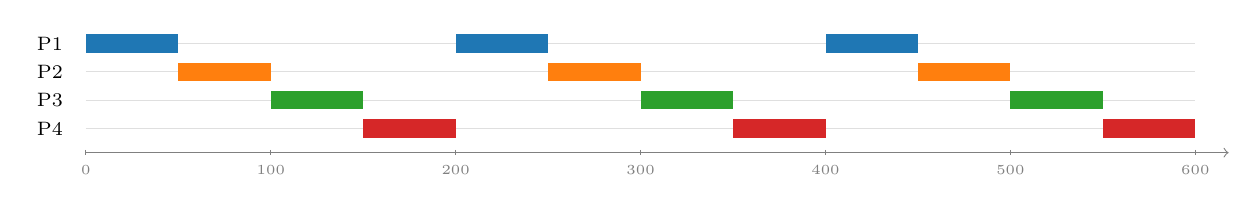
\begin{tikzpicture}[x=0.02349cm,y=0.36cm]
\node[anchor=east,font=\scriptsize] at (-7.2,3) {P1};
\draw[gray!25] (0,3) -- (600,3);
\node[anchor=east,font=\scriptsize] at (-7.2,2) {P2};
\draw[gray!25] (0,2) -- (600,2);
\node[anchor=east,font=\scriptsize] at (-7.2,1) {P3};
\draw[gray!25] (0,1) -- (600,1);
\node[anchor=east,font=\scriptsize] at (-7.2,0) {P4};
\draw[gray!25] (0,0) -- (600,0);
\fill[cP1] (0,2.68) rectangle (50,3.32);
\fill[cP2] (50,1.68) rectangle (100,2.32);
\fill[cP3] (100,0.68) rectangle (150,1.32);
\fill[cP4] (150,-0.32) rectangle (200,0.32);
\fill[cP1] (200,2.68) rectangle (250,3.32);
\fill[cP2] (250,1.68) rectangle (300,2.32);
\fill[cP3] (300,0.68) rectangle (350,1.32);
\fill[cP4] (350,-0.32) rectangle (400,0.32);
\fill[cP1] (400,2.68) rectangle (450,3.32);
\fill[cP2] (450,1.68) rectangle (500,2.32);
\fill[cP3] (500,0.68) rectangle (550,1.32);
\fill[cP4] (550,-0.32) rectangle (600,0.32);
\draw[->,gray] (0,-0.85) -- (618.0,-0.85);
\draw[gray] (0,-0.75)--(0,-0.95) node[below,font=\tiny]{0};
\draw[gray] (100,-0.75)--(100,-0.95) node[below,font=\tiny]{100};
\draw[gray] (200,-0.75)--(200,-0.95) node[below,font=\tiny]{200};
\draw[gray] (300,-0.75)--(300,-0.95) node[below,font=\tiny]{300};
\draw[gray] (400,-0.75)--(400,-0.95) node[below,font=\tiny]{400};
\draw[gray] (500,-0.75)--(500,-0.95) node[below,font=\tiny]{500};
\draw[gray] (600,-0.75)--(600,-0.95) node[below,font=\tiny]{600};
\end{tikzpicture}\par
\par\vspace{1.5mm}{\small\textbf{RR}\quad(makespan 600, idle 0)}\par\vspace{0.8mm}
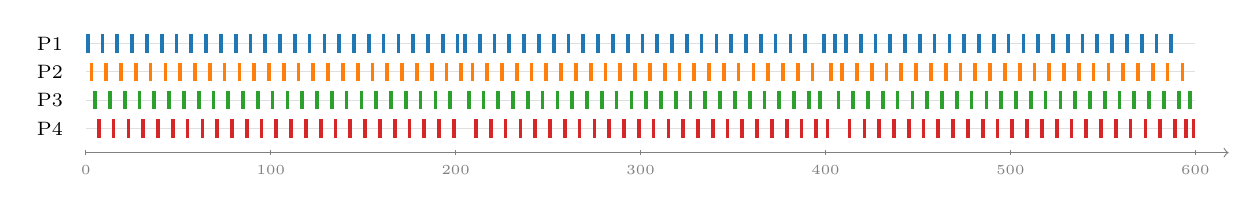
\begin{tikzpicture}[x=0.02349cm,y=0.36cm]
\node[anchor=east,font=\scriptsize] at (-7.2,3) {P1};
\draw[gray!25] (0,3) -- (600,3);
\node[anchor=east,font=\scriptsize] at (-7.2,2) {P2};
\draw[gray!25] (0,2) -- (600,2);
\node[anchor=east,font=\scriptsize] at (-7.2,1) {P3};
\draw[gray!25] (0,1) -- (600,1);
\node[anchor=east,font=\scriptsize] at (-7.2,0) {P4};
\draw[gray!25] (0,0) -- (600,0);
\fill[cP1] (0,2.68) rectangle (2,3.32);
\fill[cP2] (2,1.68) rectangle (4,2.32);
\fill[cP3] (4,0.68) rectangle (6,1.32);
\fill[cP4] (6,-0.32) rectangle (8,0.32);
\fill[cP1] (8,2.68) rectangle (10,3.32);
\fill[cP2] (10,1.68) rectangle (12,2.32);
\fill[cP3] (12,0.68) rectangle (14,1.32);
\fill[cP4] (14,-0.32) rectangle (16,0.32);
\fill[cP1] (16,2.68) rectangle (18,3.32);
\fill[cP2] (18,1.68) rectangle (20,2.32);
\fill[cP3] (20,0.68) rectangle (22,1.32);
\fill[cP4] (22,-0.32) rectangle (24,0.32);
\fill[cP1] (24,2.68) rectangle (26,3.32);
\fill[cP2] (26,1.68) rectangle (28,2.32);
\fill[cP3] (28,0.68) rectangle (30,1.32);
\fill[cP4] (30,-0.32) rectangle (32,0.32);
\fill[cP1] (32,2.68) rectangle (34,3.32);
\fill[cP2] (34,1.68) rectangle (36,2.32);
\fill[cP3] (36,0.68) rectangle (38,1.32);
\fill[cP4] (38,-0.32) rectangle (40,0.32);
\fill[cP1] (40,2.68) rectangle (42,3.32);
\fill[cP2] (42,1.68) rectangle (44,2.32);
\fill[cP3] (44,0.68) rectangle (46,1.32);
\fill[cP4] (46,-0.32) rectangle (48,0.32);
\fill[cP1] (48,2.68) rectangle (50,3.32);
\fill[cP2] (50,1.68) rectangle (52,2.32);
\fill[cP3] (52,0.68) rectangle (54,1.32);
\fill[cP4] (54,-0.32) rectangle (56,0.32);
\fill[cP1] (56,2.68) rectangle (58,3.32);
\fill[cP2] (58,1.68) rectangle (60,2.32);
\fill[cP3] (60,0.68) rectangle (62,1.32);
\fill[cP4] (62,-0.32) rectangle (64,0.32);
\fill[cP1] (64,2.68) rectangle (66,3.32);
\fill[cP2] (66,1.68) rectangle (68,2.32);
\fill[cP3] (68,0.68) rectangle (70,1.32);
\fill[cP4] (70,-0.32) rectangle (72,0.32);
\fill[cP1] (72,2.68) rectangle (74,3.32);
\fill[cP2] (74,1.68) rectangle (76,2.32);
\fill[cP3] (76,0.68) rectangle (78,1.32);
\fill[cP4] (78,-0.32) rectangle (80,0.32);
\fill[cP1] (80,2.68) rectangle (82,3.32);
\fill[cP2] (82,1.68) rectangle (84,2.32);
\fill[cP3] (84,0.68) rectangle (86,1.32);
\fill[cP4] (86,-0.32) rectangle (88,0.32);
\fill[cP1] (88,2.68) rectangle (90,3.32);
\fill[cP2] (90,1.68) rectangle (92,2.32);
\fill[cP3] (92,0.68) rectangle (94,1.32);
\fill[cP4] (94,-0.32) rectangle (96,0.32);
\fill[cP1] (96,2.68) rectangle (98,3.32);
\fill[cP2] (98,1.68) rectangle (100,2.32);
\fill[cP3] (100,0.68) rectangle (102,1.32);
\fill[cP4] (102,-0.32) rectangle (104,0.32);
\fill[cP1] (104,2.68) rectangle (106,3.32);
\fill[cP2] (106,1.68) rectangle (108,2.32);
\fill[cP3] (108,0.68) rectangle (110,1.32);
\fill[cP4] (110,-0.32) rectangle (112,0.32);
\fill[cP1] (112,2.68) rectangle (114,3.32);
\fill[cP2] (114,1.68) rectangle (116,2.32);
\fill[cP3] (116,0.68) rectangle (118,1.32);
\fill[cP4] (118,-0.32) rectangle (120,0.32);
\fill[cP1] (120,2.68) rectangle (122,3.32);
\fill[cP2] (122,1.68) rectangle (124,2.32);
\fill[cP3] (124,0.68) rectangle (126,1.32);
\fill[cP4] (126,-0.32) rectangle (128,0.32);
\fill[cP1] (128,2.68) rectangle (130,3.32);
\fill[cP2] (130,1.68) rectangle (132,2.32);
\fill[cP3] (132,0.68) rectangle (134,1.32);
\fill[cP4] (134,-0.32) rectangle (136,0.32);
\fill[cP1] (136,2.68) rectangle (138,3.32);
\fill[cP2] (138,1.68) rectangle (140,2.32);
\fill[cP3] (140,0.68) rectangle (142,1.32);
\fill[cP4] (142,-0.32) rectangle (144,0.32);
\fill[cP1] (144,2.68) rectangle (146,3.32);
\fill[cP2] (146,1.68) rectangle (148,2.32);
\fill[cP3] (148,0.68) rectangle (150,1.32);
\fill[cP4] (150,-0.32) rectangle (152,0.32);
\fill[cP1] (152,2.68) rectangle (154,3.32);
\fill[cP2] (154,1.68) rectangle (156,2.32);
\fill[cP3] (156,0.68) rectangle (158,1.32);
\fill[cP4] (158,-0.32) rectangle (160,0.32);
\fill[cP1] (160,2.68) rectangle (162,3.32);
\fill[cP2] (162,1.68) rectangle (164,2.32);
\fill[cP3] (164,0.68) rectangle (166,1.32);
\fill[cP4] (166,-0.32) rectangle (168,0.32);
\fill[cP1] (168,2.68) rectangle (170,3.32);
\fill[cP2] (170,1.68) rectangle (172,2.32);
\fill[cP3] (172,0.68) rectangle (174,1.32);
\fill[cP4] (174,-0.32) rectangle (176,0.32);
\fill[cP1] (176,2.68) rectangle (178,3.32);
\fill[cP2] (178,1.68) rectangle (180,2.32);
\fill[cP3] (180,0.68) rectangle (182,1.32);
\fill[cP4] (182,-0.32) rectangle (184,0.32);
\fill[cP1] (184,2.68) rectangle (186,3.32);
\fill[cP2] (186,1.68) rectangle (188,2.32);
\fill[cP3] (188,0.68) rectangle (190,1.32);
\fill[cP4] (190,-0.32) rectangle (192,0.32);
\fill[cP1] (192,2.68) rectangle (194,3.32);
\fill[cP2] (194,1.68) rectangle (196,2.32);
\fill[cP3] (196,0.68) rectangle (198,1.32);
\fill[cP4] (198,-0.32) rectangle (200,0.32);
\fill[cP1] (200,2.68) rectangle (202,3.32);
\fill[cP2] (202,1.68) rectangle (204,2.32);
\fill[cP1] (204,2.68) rectangle (206,3.32);
\fill[cP3] (206,0.68) rectangle (208,1.32);
\fill[cP2] (208,1.68) rectangle (210,2.32);
\fill[cP4] (210,-0.32) rectangle (212,0.32);
\fill[cP1] (212,2.68) rectangle (214,3.32);
\fill[cP3] (214,0.68) rectangle (216,1.32);
\fill[cP2] (216,1.68) rectangle (218,2.32);
\fill[cP4] (218,-0.32) rectangle (220,0.32);
\fill[cP1] (220,2.68) rectangle (222,3.32);
\fill[cP3] (222,0.68) rectangle (224,1.32);
\fill[cP2] (224,1.68) rectangle (226,2.32);
\fill[cP4] (226,-0.32) rectangle (228,0.32);
\fill[cP1] (228,2.68) rectangle (230,3.32);
\fill[cP3] (230,0.68) rectangle (232,1.32);
\fill[cP2] (232,1.68) rectangle (234,2.32);
\fill[cP4] (234,-0.32) rectangle (236,0.32);
\fill[cP1] (236,2.68) rectangle (238,3.32);
\fill[cP3] (238,0.68) rectangle (240,1.32);
\fill[cP2] (240,1.68) rectangle (242,2.32);
\fill[cP4] (242,-0.32) rectangle (244,0.32);
\fill[cP1] (244,2.68) rectangle (246,3.32);
\fill[cP3] (246,0.68) rectangle (248,1.32);
\fill[cP2] (248,1.68) rectangle (250,2.32);
\fill[cP4] (250,-0.32) rectangle (252,0.32);
\fill[cP1] (252,2.68) rectangle (254,3.32);
\fill[cP3] (254,0.68) rectangle (256,1.32);
\fill[cP2] (256,1.68) rectangle (258,2.32);
\fill[cP4] (258,-0.32) rectangle (260,0.32);
\fill[cP1] (260,2.68) rectangle (262,3.32);
\fill[cP3] (262,0.68) rectangle (264,1.32);
\fill[cP2] (264,1.68) rectangle (266,2.32);
\fill[cP4] (266,-0.32) rectangle (268,0.32);
\fill[cP1] (268,2.68) rectangle (270,3.32);
\fill[cP3] (270,0.68) rectangle (272,1.32);
\fill[cP2] (272,1.68) rectangle (274,2.32);
\fill[cP4] (274,-0.32) rectangle (276,0.32);
\fill[cP1] (276,2.68) rectangle (278,3.32);
\fill[cP3] (278,0.68) rectangle (280,1.32);
\fill[cP2] (280,1.68) rectangle (282,2.32);
\fill[cP4] (282,-0.32) rectangle (284,0.32);
\fill[cP1] (284,2.68) rectangle (286,3.32);
\fill[cP3] (286,0.68) rectangle (288,1.32);
\fill[cP2] (288,1.68) rectangle (290,2.32);
\fill[cP4] (290,-0.32) rectangle (292,0.32);
\fill[cP1] (292,2.68) rectangle (294,3.32);
\fill[cP3] (294,0.68) rectangle (296,1.32);
\fill[cP2] (296,1.68) rectangle (298,2.32);
\fill[cP4] (298,-0.32) rectangle (300,0.32);
\fill[cP1] (300,2.68) rectangle (302,3.32);
\fill[cP3] (302,0.68) rectangle (304,1.32);
\fill[cP2] (304,1.68) rectangle (306,2.32);
\fill[cP4] (306,-0.32) rectangle (308,0.32);
\fill[cP1] (308,2.68) rectangle (310,3.32);
\fill[cP3] (310,0.68) rectangle (312,1.32);
\fill[cP2] (312,1.68) rectangle (314,2.32);
\fill[cP4] (314,-0.32) rectangle (316,0.32);
\fill[cP1] (316,2.68) rectangle (318,3.32);
\fill[cP3] (318,0.68) rectangle (320,1.32);
\fill[cP2] (320,1.68) rectangle (322,2.32);
\fill[cP4] (322,-0.32) rectangle (324,0.32);
\fill[cP1] (324,2.68) rectangle (326,3.32);
\fill[cP3] (326,0.68) rectangle (328,1.32);
\fill[cP2] (328,1.68) rectangle (330,2.32);
\fill[cP4] (330,-0.32) rectangle (332,0.32);
\fill[cP1] (332,2.68) rectangle (334,3.32);
\fill[cP3] (334,0.68) rectangle (336,1.32);
\fill[cP2] (336,1.68) rectangle (338,2.32);
\fill[cP4] (338,-0.32) rectangle (340,0.32);
\fill[cP1] (340,2.68) rectangle (342,3.32);
\fill[cP3] (342,0.68) rectangle (344,1.32);
\fill[cP2] (344,1.68) rectangle (346,2.32);
\fill[cP4] (346,-0.32) rectangle (348,0.32);
\fill[cP1] (348,2.68) rectangle (350,3.32);
\fill[cP3] (350,0.68) rectangle (352,1.32);
\fill[cP2] (352,1.68) rectangle (354,2.32);
\fill[cP4] (354,-0.32) rectangle (356,0.32);
\fill[cP1] (356,2.68) rectangle (358,3.32);
\fill[cP3] (358,0.68) rectangle (360,1.32);
\fill[cP2] (360,1.68) rectangle (362,2.32);
\fill[cP4] (362,-0.32) rectangle (364,0.32);
\fill[cP1] (364,2.68) rectangle (366,3.32);
\fill[cP3] (366,0.68) rectangle (368,1.32);
\fill[cP2] (368,1.68) rectangle (370,2.32);
\fill[cP4] (370,-0.32) rectangle (372,0.32);
\fill[cP1] (372,2.68) rectangle (374,3.32);
\fill[cP3] (374,0.68) rectangle (376,1.32);
\fill[cP2] (376,1.68) rectangle (378,2.32);
\fill[cP4] (378,-0.32) rectangle (380,0.32);
\fill[cP1] (380,2.68) rectangle (382,3.32);
\fill[cP3] (382,0.68) rectangle (384,1.32);
\fill[cP2] (384,1.68) rectangle (386,2.32);
\fill[cP4] (386,-0.32) rectangle (388,0.32);
\fill[cP1] (388,2.68) rectangle (390,3.32);
\fill[cP3] (390,0.68) rectangle (392,1.32);
\fill[cP2] (392,1.68) rectangle (394,2.32);
\fill[cP4] (394,-0.32) rectangle (396,0.32);
\fill[cP3] (396,0.68) rectangle (398,1.32);
\fill[cP1] (398,2.68) rectangle (400,3.32);
\fill[cP4] (400,-0.32) rectangle (402,0.32);
\fill[cP2] (402,1.68) rectangle (404,2.32);
\fill[cP1] (404,2.68) rectangle (406,3.32);
\fill[cP3] (406,0.68) rectangle (408,1.32);
\fill[cP2] (408,1.68) rectangle (410,2.32);
\fill[cP1] (410,2.68) rectangle (412,3.32);
\fill[cP4] (412,-0.32) rectangle (414,0.32);
\fill[cP3] (414,0.68) rectangle (416,1.32);
\fill[cP2] (416,1.68) rectangle (418,2.32);
\fill[cP1] (418,2.68) rectangle (420,3.32);
\fill[cP4] (420,-0.32) rectangle (422,0.32);
\fill[cP3] (422,0.68) rectangle (424,1.32);
\fill[cP2] (424,1.68) rectangle (426,2.32);
\fill[cP1] (426,2.68) rectangle (428,3.32);
\fill[cP4] (428,-0.32) rectangle (430,0.32);
\fill[cP3] (430,0.68) rectangle (432,1.32);
\fill[cP2] (432,1.68) rectangle (434,2.32);
\fill[cP1] (434,2.68) rectangle (436,3.32);
\fill[cP4] (436,-0.32) rectangle (438,0.32);
\fill[cP3] (438,0.68) rectangle (440,1.32);
\fill[cP2] (440,1.68) rectangle (442,2.32);
\fill[cP1] (442,2.68) rectangle (444,3.32);
\fill[cP4] (444,-0.32) rectangle (446,0.32);
\fill[cP3] (446,0.68) rectangle (448,1.32);
\fill[cP2] (448,1.68) rectangle (450,2.32);
\fill[cP1] (450,2.68) rectangle (452,3.32);
\fill[cP4] (452,-0.32) rectangle (454,0.32);
\fill[cP3] (454,0.68) rectangle (456,1.32);
\fill[cP2] (456,1.68) rectangle (458,2.32);
\fill[cP1] (458,2.68) rectangle (460,3.32);
\fill[cP4] (460,-0.32) rectangle (462,0.32);
\fill[cP3] (462,0.68) rectangle (464,1.32);
\fill[cP2] (464,1.68) rectangle (466,2.32);
\fill[cP1] (466,2.68) rectangle (468,3.32);
\fill[cP4] (468,-0.32) rectangle (470,0.32);
\fill[cP3] (470,0.68) rectangle (472,1.32);
\fill[cP2] (472,1.68) rectangle (474,2.32);
\fill[cP1] (474,2.68) rectangle (476,3.32);
\fill[cP4] (476,-0.32) rectangle (478,0.32);
\fill[cP3] (478,0.68) rectangle (480,1.32);
\fill[cP2] (480,1.68) rectangle (482,2.32);
\fill[cP1] (482,2.68) rectangle (484,3.32);
\fill[cP4] (484,-0.32) rectangle (486,0.32);
\fill[cP3] (486,0.68) rectangle (488,1.32);
\fill[cP2] (488,1.68) rectangle (490,2.32);
\fill[cP1] (490,2.68) rectangle (492,3.32);
\fill[cP4] (492,-0.32) rectangle (494,0.32);
\fill[cP3] (494,0.68) rectangle (496,1.32);
\fill[cP2] (496,1.68) rectangle (498,2.32);
\fill[cP1] (498,2.68) rectangle (500,3.32);
\fill[cP4] (500,-0.32) rectangle (502,0.32);
\fill[cP3] (502,0.68) rectangle (504,1.32);
\fill[cP2] (504,1.68) rectangle (506,2.32);
\fill[cP1] (506,2.68) rectangle (508,3.32);
\fill[cP4] (508,-0.32) rectangle (510,0.32);
\fill[cP3] (510,0.68) rectangle (512,1.32);
\fill[cP2] (512,1.68) rectangle (514,2.32);
\fill[cP1] (514,2.68) rectangle (516,3.32);
\fill[cP4] (516,-0.32) rectangle (518,0.32);
\fill[cP3] (518,0.68) rectangle (520,1.32);
\fill[cP2] (520,1.68) rectangle (522,2.32);
\fill[cP1] (522,2.68) rectangle (524,3.32);
\fill[cP4] (524,-0.32) rectangle (526,0.32);
\fill[cP3] (526,0.68) rectangle (528,1.32);
\fill[cP2] (528,1.68) rectangle (530,2.32);
\fill[cP1] (530,2.68) rectangle (532,3.32);
\fill[cP4] (532,-0.32) rectangle (534,0.32);
\fill[cP3] (534,0.68) rectangle (536,1.32);
\fill[cP2] (536,1.68) rectangle (538,2.32);
\fill[cP1] (538,2.68) rectangle (540,3.32);
\fill[cP4] (540,-0.32) rectangle (542,0.32);
\fill[cP3] (542,0.68) rectangle (544,1.32);
\fill[cP2] (544,1.68) rectangle (546,2.32);
\fill[cP1] (546,2.68) rectangle (548,3.32);
\fill[cP4] (548,-0.32) rectangle (550,0.32);
\fill[cP3] (550,0.68) rectangle (552,1.32);
\fill[cP2] (552,1.68) rectangle (554,2.32);
\fill[cP1] (554,2.68) rectangle (556,3.32);
\fill[cP4] (556,-0.32) rectangle (558,0.32);
\fill[cP3] (558,0.68) rectangle (560,1.32);
\fill[cP2] (560,1.68) rectangle (562,2.32);
\fill[cP1] (562,2.68) rectangle (564,3.32);
\fill[cP4] (564,-0.32) rectangle (566,0.32);
\fill[cP3] (566,0.68) rectangle (568,1.32);
\fill[cP2] (568,1.68) rectangle (570,2.32);
\fill[cP1] (570,2.68) rectangle (572,3.32);
\fill[cP4] (572,-0.32) rectangle (574,0.32);
\fill[cP3] (574,0.68) rectangle (576,1.32);
\fill[cP2] (576,1.68) rectangle (578,2.32);
\fill[cP1] (578,2.68) rectangle (580,3.32);
\fill[cP4] (580,-0.32) rectangle (582,0.32);
\fill[cP3] (582,0.68) rectangle (584,1.32);
\fill[cP2] (584,1.68) rectangle (586,2.32);
\fill[cP1] (586,2.68) rectangle (588,3.32);
\fill[cP4] (588,-0.32) rectangle (590,0.32);
\fill[cP3] (590,0.68) rectangle (592,1.32);
\fill[cP2] (592,1.68) rectangle (594,2.32);
\fill[cP4] (594,-0.32) rectangle (596,0.32);
\fill[cP3] (596,0.68) rectangle (598,1.32);
\fill[cP4] (598,-0.32) rectangle (600,0.32);
\draw[->,gray] (0,-0.85) -- (618.0,-0.85);
\draw[gray] (0,-0.75)--(0,-0.95) node[below,font=\tiny]{0};
\draw[gray] (100,-0.75)--(100,-0.95) node[below,font=\tiny]{100};
\draw[gray] (200,-0.75)--(200,-0.95) node[below,font=\tiny]{200};
\draw[gray] (300,-0.75)--(300,-0.95) node[below,font=\tiny]{300};
\draw[gray] (400,-0.75)--(400,-0.95) node[below,font=\tiny]{400};
\draw[gray] (500,-0.75)--(500,-0.95) node[below,font=\tiny]{500};
\draw[gray] (600,-0.75)--(600,-0.95) node[below,font=\tiny]{600};
\end{tikzpicture}\par
\par\vspace{1.5mm}{\small\textbf{MLFQ-NB}\quad(makespan 600, idle 0)}\par\vspace{0.8mm}
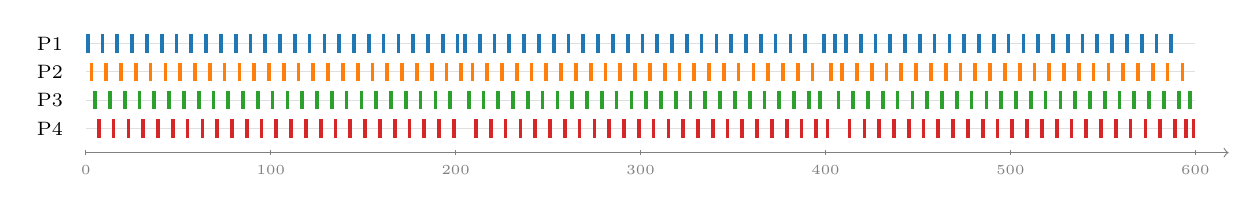
\begin{tikzpicture}[x=0.02349cm,y=0.36cm]
\node[anchor=east,font=\scriptsize] at (-7.2,3) {P1};
\draw[gray!25] (0,3) -- (600,3);
\node[anchor=east,font=\scriptsize] at (-7.2,2) {P2};
\draw[gray!25] (0,2) -- (600,2);
\node[anchor=east,font=\scriptsize] at (-7.2,1) {P3};
\draw[gray!25] (0,1) -- (600,1);
\node[anchor=east,font=\scriptsize] at (-7.2,0) {P4};
\draw[gray!25] (0,0) -- (600,0);
\fill[cP1] (0,2.68) rectangle (2,3.32);
\fill[cP2] (2,1.68) rectangle (4,2.32);
\fill[cP3] (4,0.68) rectangle (6,1.32);
\fill[cP4] (6,-0.32) rectangle (8,0.32);
\fill[cP1] (8,2.68) rectangle (10,3.32);
\fill[cP2] (10,1.68) rectangle (12,2.32);
\fill[cP3] (12,0.68) rectangle (14,1.32);
\fill[cP4] (14,-0.32) rectangle (16,0.32);
\fill[cP1] (16,2.68) rectangle (18,3.32);
\fill[cP2] (18,1.68) rectangle (20,2.32);
\fill[cP3] (20,0.68) rectangle (22,1.32);
\fill[cP4] (22,-0.32) rectangle (24,0.32);
\fill[cP1] (24,2.68) rectangle (26,3.32);
\fill[cP2] (26,1.68) rectangle (28,2.32);
\fill[cP3] (28,0.68) rectangle (30,1.32);
\fill[cP4] (30,-0.32) rectangle (32,0.32);
\fill[cP1] (32,2.68) rectangle (34,3.32);
\fill[cP2] (34,1.68) rectangle (36,2.32);
\fill[cP3] (36,0.68) rectangle (38,1.32);
\fill[cP4] (38,-0.32) rectangle (40,0.32);
\fill[cP1] (40,2.68) rectangle (42,3.32);
\fill[cP2] (42,1.68) rectangle (44,2.32);
\fill[cP3] (44,0.68) rectangle (46,1.32);
\fill[cP4] (46,-0.32) rectangle (48,0.32);
\fill[cP1] (48,2.68) rectangle (50,3.32);
\fill[cP2] (50,1.68) rectangle (52,2.32);
\fill[cP3] (52,0.68) rectangle (54,1.32);
\fill[cP4] (54,-0.32) rectangle (56,0.32);
\fill[cP1] (56,2.68) rectangle (58,3.32);
\fill[cP2] (58,1.68) rectangle (60,2.32);
\fill[cP3] (60,0.68) rectangle (62,1.32);
\fill[cP4] (62,-0.32) rectangle (64,0.32);
\fill[cP1] (64,2.68) rectangle (66,3.32);
\fill[cP2] (66,1.68) rectangle (68,2.32);
\fill[cP3] (68,0.68) rectangle (70,1.32);
\fill[cP4] (70,-0.32) rectangle (72,0.32);
\fill[cP1] (72,2.68) rectangle (74,3.32);
\fill[cP2] (74,1.68) rectangle (76,2.32);
\fill[cP3] (76,0.68) rectangle (78,1.32);
\fill[cP4] (78,-0.32) rectangle (80,0.32);
\fill[cP1] (80,2.68) rectangle (82,3.32);
\fill[cP2] (82,1.68) rectangle (84,2.32);
\fill[cP3] (84,0.68) rectangle (86,1.32);
\fill[cP4] (86,-0.32) rectangle (88,0.32);
\fill[cP1] (88,2.68) rectangle (90,3.32);
\fill[cP2] (90,1.68) rectangle (92,2.32);
\fill[cP3] (92,0.68) rectangle (94,1.32);
\fill[cP4] (94,-0.32) rectangle (96,0.32);
\fill[cP1] (96,2.68) rectangle (98,3.32);
\fill[cP2] (98,1.68) rectangle (100,2.32);
\fill[cP3] (100,0.68) rectangle (102,1.32);
\fill[cP4] (102,-0.32) rectangle (104,0.32);
\fill[cP1] (104,2.68) rectangle (106,3.32);
\fill[cP2] (106,1.68) rectangle (108,2.32);
\fill[cP3] (108,0.68) rectangle (110,1.32);
\fill[cP4] (110,-0.32) rectangle (112,0.32);
\fill[cP1] (112,2.68) rectangle (114,3.32);
\fill[cP2] (114,1.68) rectangle (116,2.32);
\fill[cP3] (116,0.68) rectangle (118,1.32);
\fill[cP4] (118,-0.32) rectangle (120,0.32);
\fill[cP1] (120,2.68) rectangle (122,3.32);
\fill[cP2] (122,1.68) rectangle (124,2.32);
\fill[cP3] (124,0.68) rectangle (126,1.32);
\fill[cP4] (126,-0.32) rectangle (128,0.32);
\fill[cP1] (128,2.68) rectangle (130,3.32);
\fill[cP2] (130,1.68) rectangle (132,2.32);
\fill[cP3] (132,0.68) rectangle (134,1.32);
\fill[cP4] (134,-0.32) rectangle (136,0.32);
\fill[cP1] (136,2.68) rectangle (138,3.32);
\fill[cP2] (138,1.68) rectangle (140,2.32);
\fill[cP3] (140,0.68) rectangle (142,1.32);
\fill[cP4] (142,-0.32) rectangle (144,0.32);
\fill[cP1] (144,2.68) rectangle (146,3.32);
\fill[cP2] (146,1.68) rectangle (148,2.32);
\fill[cP3] (148,0.68) rectangle (150,1.32);
\fill[cP4] (150,-0.32) rectangle (152,0.32);
\fill[cP1] (152,2.68) rectangle (154,3.32);
\fill[cP2] (154,1.68) rectangle (156,2.32);
\fill[cP3] (156,0.68) rectangle (158,1.32);
\fill[cP4] (158,-0.32) rectangle (160,0.32);
\fill[cP1] (160,2.68) rectangle (162,3.32);
\fill[cP2] (162,1.68) rectangle (164,2.32);
\fill[cP3] (164,0.68) rectangle (166,1.32);
\fill[cP4] (166,-0.32) rectangle (168,0.32);
\fill[cP1] (168,2.68) rectangle (170,3.32);
\fill[cP2] (170,1.68) rectangle (172,2.32);
\fill[cP3] (172,0.68) rectangle (174,1.32);
\fill[cP4] (174,-0.32) rectangle (176,0.32);
\fill[cP1] (176,2.68) rectangle (178,3.32);
\fill[cP2] (178,1.68) rectangle (180,2.32);
\fill[cP3] (180,0.68) rectangle (182,1.32);
\fill[cP4] (182,-0.32) rectangle (184,0.32);
\fill[cP1] (184,2.68) rectangle (186,3.32);
\fill[cP2] (186,1.68) rectangle (188,2.32);
\fill[cP3] (188,0.68) rectangle (190,1.32);
\fill[cP4] (190,-0.32) rectangle (192,0.32);
\fill[cP1] (192,2.68) rectangle (194,3.32);
\fill[cP2] (194,1.68) rectangle (196,2.32);
\fill[cP3] (196,0.68) rectangle (198,1.32);
\fill[cP4] (198,-0.32) rectangle (200,0.32);
\fill[cP1] (200,2.68) rectangle (202,3.32);
\fill[cP2] (202,1.68) rectangle (204,2.32);
\fill[cP1] (204,2.68) rectangle (206,3.32);
\fill[cP3] (206,0.68) rectangle (208,1.32);
\fill[cP2] (208,1.68) rectangle (210,2.32);
\fill[cP4] (210,-0.32) rectangle (212,0.32);
\fill[cP1] (212,2.68) rectangle (214,3.32);
\fill[cP3] (214,0.68) rectangle (216,1.32);
\fill[cP2] (216,1.68) rectangle (218,2.32);
\fill[cP4] (218,-0.32) rectangle (220,0.32);
\fill[cP1] (220,2.68) rectangle (222,3.32);
\fill[cP3] (222,0.68) rectangle (224,1.32);
\fill[cP2] (224,1.68) rectangle (226,2.32);
\fill[cP4] (226,-0.32) rectangle (228,0.32);
\fill[cP1] (228,2.68) rectangle (230,3.32);
\fill[cP3] (230,0.68) rectangle (232,1.32);
\fill[cP2] (232,1.68) rectangle (234,2.32);
\fill[cP4] (234,-0.32) rectangle (236,0.32);
\fill[cP1] (236,2.68) rectangle (238,3.32);
\fill[cP3] (238,0.68) rectangle (240,1.32);
\fill[cP2] (240,1.68) rectangle (242,2.32);
\fill[cP4] (242,-0.32) rectangle (244,0.32);
\fill[cP1] (244,2.68) rectangle (246,3.32);
\fill[cP3] (246,0.68) rectangle (248,1.32);
\fill[cP2] (248,1.68) rectangle (250,2.32);
\fill[cP4] (250,-0.32) rectangle (252,0.32);
\fill[cP1] (252,2.68) rectangle (254,3.32);
\fill[cP3] (254,0.68) rectangle (256,1.32);
\fill[cP2] (256,1.68) rectangle (258,2.32);
\fill[cP4] (258,-0.32) rectangle (260,0.32);
\fill[cP1] (260,2.68) rectangle (262,3.32);
\fill[cP3] (262,0.68) rectangle (264,1.32);
\fill[cP2] (264,1.68) rectangle (266,2.32);
\fill[cP4] (266,-0.32) rectangle (268,0.32);
\fill[cP1] (268,2.68) rectangle (270,3.32);
\fill[cP3] (270,0.68) rectangle (272,1.32);
\fill[cP2] (272,1.68) rectangle (274,2.32);
\fill[cP4] (274,-0.32) rectangle (276,0.32);
\fill[cP1] (276,2.68) rectangle (278,3.32);
\fill[cP3] (278,0.68) rectangle (280,1.32);
\fill[cP2] (280,1.68) rectangle (282,2.32);
\fill[cP4] (282,-0.32) rectangle (284,0.32);
\fill[cP1] (284,2.68) rectangle (286,3.32);
\fill[cP3] (286,0.68) rectangle (288,1.32);
\fill[cP2] (288,1.68) rectangle (290,2.32);
\fill[cP4] (290,-0.32) rectangle (292,0.32);
\fill[cP1] (292,2.68) rectangle (294,3.32);
\fill[cP3] (294,0.68) rectangle (296,1.32);
\fill[cP2] (296,1.68) rectangle (298,2.32);
\fill[cP4] (298,-0.32) rectangle (300,0.32);
\fill[cP1] (300,2.68) rectangle (302,3.32);
\fill[cP3] (302,0.68) rectangle (304,1.32);
\fill[cP2] (304,1.68) rectangle (306,2.32);
\fill[cP4] (306,-0.32) rectangle (308,0.32);
\fill[cP1] (308,2.68) rectangle (310,3.32);
\fill[cP3] (310,0.68) rectangle (312,1.32);
\fill[cP2] (312,1.68) rectangle (314,2.32);
\fill[cP4] (314,-0.32) rectangle (316,0.32);
\fill[cP1] (316,2.68) rectangle (318,3.32);
\fill[cP3] (318,0.68) rectangle (320,1.32);
\fill[cP2] (320,1.68) rectangle (322,2.32);
\fill[cP4] (322,-0.32) rectangle (324,0.32);
\fill[cP1] (324,2.68) rectangle (326,3.32);
\fill[cP3] (326,0.68) rectangle (328,1.32);
\fill[cP2] (328,1.68) rectangle (330,2.32);
\fill[cP4] (330,-0.32) rectangle (332,0.32);
\fill[cP1] (332,2.68) rectangle (334,3.32);
\fill[cP3] (334,0.68) rectangle (336,1.32);
\fill[cP2] (336,1.68) rectangle (338,2.32);
\fill[cP4] (338,-0.32) rectangle (340,0.32);
\fill[cP1] (340,2.68) rectangle (342,3.32);
\fill[cP3] (342,0.68) rectangle (344,1.32);
\fill[cP2] (344,1.68) rectangle (346,2.32);
\fill[cP4] (346,-0.32) rectangle (348,0.32);
\fill[cP1] (348,2.68) rectangle (350,3.32);
\fill[cP3] (350,0.68) rectangle (352,1.32);
\fill[cP2] (352,1.68) rectangle (354,2.32);
\fill[cP4] (354,-0.32) rectangle (356,0.32);
\fill[cP1] (356,2.68) rectangle (358,3.32);
\fill[cP3] (358,0.68) rectangle (360,1.32);
\fill[cP2] (360,1.68) rectangle (362,2.32);
\fill[cP4] (362,-0.32) rectangle (364,0.32);
\fill[cP1] (364,2.68) rectangle (366,3.32);
\fill[cP3] (366,0.68) rectangle (368,1.32);
\fill[cP2] (368,1.68) rectangle (370,2.32);
\fill[cP4] (370,-0.32) rectangle (372,0.32);
\fill[cP1] (372,2.68) rectangle (374,3.32);
\fill[cP3] (374,0.68) rectangle (376,1.32);
\fill[cP2] (376,1.68) rectangle (378,2.32);
\fill[cP4] (378,-0.32) rectangle (380,0.32);
\fill[cP1] (380,2.68) rectangle (382,3.32);
\fill[cP3] (382,0.68) rectangle (384,1.32);
\fill[cP2] (384,1.68) rectangle (386,2.32);
\fill[cP4] (386,-0.32) rectangle (388,0.32);
\fill[cP1] (388,2.68) rectangle (390,3.32);
\fill[cP3] (390,0.68) rectangle (392,1.32);
\fill[cP2] (392,1.68) rectangle (394,2.32);
\fill[cP4] (394,-0.32) rectangle (396,0.32);
\fill[cP3] (396,0.68) rectangle (398,1.32);
\fill[cP1] (398,2.68) rectangle (400,3.32);
\fill[cP4] (400,-0.32) rectangle (402,0.32);
\fill[cP2] (402,1.68) rectangle (404,2.32);
\fill[cP1] (404,2.68) rectangle (406,3.32);
\fill[cP3] (406,0.68) rectangle (408,1.32);
\fill[cP2] (408,1.68) rectangle (410,2.32);
\fill[cP1] (410,2.68) rectangle (412,3.32);
\fill[cP4] (412,-0.32) rectangle (414,0.32);
\fill[cP3] (414,0.68) rectangle (416,1.32);
\fill[cP2] (416,1.68) rectangle (418,2.32);
\fill[cP1] (418,2.68) rectangle (420,3.32);
\fill[cP4] (420,-0.32) rectangle (422,0.32);
\fill[cP3] (422,0.68) rectangle (424,1.32);
\fill[cP2] (424,1.68) rectangle (426,2.32);
\fill[cP1] (426,2.68) rectangle (428,3.32);
\fill[cP4] (428,-0.32) rectangle (430,0.32);
\fill[cP3] (430,0.68) rectangle (432,1.32);
\fill[cP2] (432,1.68) rectangle (434,2.32);
\fill[cP1] (434,2.68) rectangle (436,3.32);
\fill[cP4] (436,-0.32) rectangle (438,0.32);
\fill[cP3] (438,0.68) rectangle (440,1.32);
\fill[cP2] (440,1.68) rectangle (442,2.32);
\fill[cP1] (442,2.68) rectangle (444,3.32);
\fill[cP4] (444,-0.32) rectangle (446,0.32);
\fill[cP3] (446,0.68) rectangle (448,1.32);
\fill[cP2] (448,1.68) rectangle (450,2.32);
\fill[cP1] (450,2.68) rectangle (452,3.32);
\fill[cP4] (452,-0.32) rectangle (454,0.32);
\fill[cP3] (454,0.68) rectangle (456,1.32);
\fill[cP2] (456,1.68) rectangle (458,2.32);
\fill[cP1] (458,2.68) rectangle (460,3.32);
\fill[cP4] (460,-0.32) rectangle (462,0.32);
\fill[cP3] (462,0.68) rectangle (464,1.32);
\fill[cP2] (464,1.68) rectangle (466,2.32);
\fill[cP1] (466,2.68) rectangle (468,3.32);
\fill[cP4] (468,-0.32) rectangle (470,0.32);
\fill[cP3] (470,0.68) rectangle (472,1.32);
\fill[cP2] (472,1.68) rectangle (474,2.32);
\fill[cP1] (474,2.68) rectangle (476,3.32);
\fill[cP4] (476,-0.32) rectangle (478,0.32);
\fill[cP3] (478,0.68) rectangle (480,1.32);
\fill[cP2] (480,1.68) rectangle (482,2.32);
\fill[cP1] (482,2.68) rectangle (484,3.32);
\fill[cP4] (484,-0.32) rectangle (486,0.32);
\fill[cP3] (486,0.68) rectangle (488,1.32);
\fill[cP2] (488,1.68) rectangle (490,2.32);
\fill[cP1] (490,2.68) rectangle (492,3.32);
\fill[cP4] (492,-0.32) rectangle (494,0.32);
\fill[cP3] (494,0.68) rectangle (496,1.32);
\fill[cP2] (496,1.68) rectangle (498,2.32);
\fill[cP1] (498,2.68) rectangle (500,3.32);
\fill[cP4] (500,-0.32) rectangle (502,0.32);
\fill[cP3] (502,0.68) rectangle (504,1.32);
\fill[cP2] (504,1.68) rectangle (506,2.32);
\fill[cP1] (506,2.68) rectangle (508,3.32);
\fill[cP4] (508,-0.32) rectangle (510,0.32);
\fill[cP3] (510,0.68) rectangle (512,1.32);
\fill[cP2] (512,1.68) rectangle (514,2.32);
\fill[cP1] (514,2.68) rectangle (516,3.32);
\fill[cP4] (516,-0.32) rectangle (518,0.32);
\fill[cP3] (518,0.68) rectangle (520,1.32);
\fill[cP2] (520,1.68) rectangle (522,2.32);
\fill[cP1] (522,2.68) rectangle (524,3.32);
\fill[cP4] (524,-0.32) rectangle (526,0.32);
\fill[cP3] (526,0.68) rectangle (528,1.32);
\fill[cP2] (528,1.68) rectangle (530,2.32);
\fill[cP1] (530,2.68) rectangle (532,3.32);
\fill[cP4] (532,-0.32) rectangle (534,0.32);
\fill[cP3] (534,0.68) rectangle (536,1.32);
\fill[cP2] (536,1.68) rectangle (538,2.32);
\fill[cP1] (538,2.68) rectangle (540,3.32);
\fill[cP4] (540,-0.32) rectangle (542,0.32);
\fill[cP3] (542,0.68) rectangle (544,1.32);
\fill[cP2] (544,1.68) rectangle (546,2.32);
\fill[cP1] (546,2.68) rectangle (548,3.32);
\fill[cP4] (548,-0.32) rectangle (550,0.32);
\fill[cP3] (550,0.68) rectangle (552,1.32);
\fill[cP2] (552,1.68) rectangle (554,2.32);
\fill[cP1] (554,2.68) rectangle (556,3.32);
\fill[cP4] (556,-0.32) rectangle (558,0.32);
\fill[cP3] (558,0.68) rectangle (560,1.32);
\fill[cP2] (560,1.68) rectangle (562,2.32);
\fill[cP1] (562,2.68) rectangle (564,3.32);
\fill[cP4] (564,-0.32) rectangle (566,0.32);
\fill[cP3] (566,0.68) rectangle (568,1.32);
\fill[cP2] (568,1.68) rectangle (570,2.32);
\fill[cP1] (570,2.68) rectangle (572,3.32);
\fill[cP4] (572,-0.32) rectangle (574,0.32);
\fill[cP3] (574,0.68) rectangle (576,1.32);
\fill[cP2] (576,1.68) rectangle (578,2.32);
\fill[cP1] (578,2.68) rectangle (580,3.32);
\fill[cP4] (580,-0.32) rectangle (582,0.32);
\fill[cP3] (582,0.68) rectangle (584,1.32);
\fill[cP2] (584,1.68) rectangle (586,2.32);
\fill[cP1] (586,2.68) rectangle (588,3.32);
\fill[cP4] (588,-0.32) rectangle (590,0.32);
\fill[cP3] (590,0.68) rectangle (592,1.32);
\fill[cP2] (592,1.68) rectangle (594,2.32);
\fill[cP4] (594,-0.32) rectangle (596,0.32);
\fill[cP3] (596,0.68) rectangle (598,1.32);
\fill[cP4] (598,-0.32) rectangle (600,0.32);
\draw[->,gray] (0,-0.85) -- (618.0,-0.85);
\draw[gray] (0,-0.75)--(0,-0.95) node[below,font=\tiny]{0};
\draw[gray] (100,-0.75)--(100,-0.95) node[below,font=\tiny]{100};
\draw[gray] (200,-0.75)--(200,-0.95) node[below,font=\tiny]{200};
\draw[gray] (300,-0.75)--(300,-0.95) node[below,font=\tiny]{300};
\draw[gray] (400,-0.75)--(400,-0.95) node[below,font=\tiny]{400};
\draw[gray] (500,-0.75)--(500,-0.95) node[below,font=\tiny]{500};
\draw[gray] (600,-0.75)--(600,-0.95) node[below,font=\tiny]{600};
\end{tikzpicture}\par
\par\vspace{1.5mm}{\small\textbf{MLFQ-WB}\quad(makespan 600, idle 0)}\par\vspace{0.8mm}
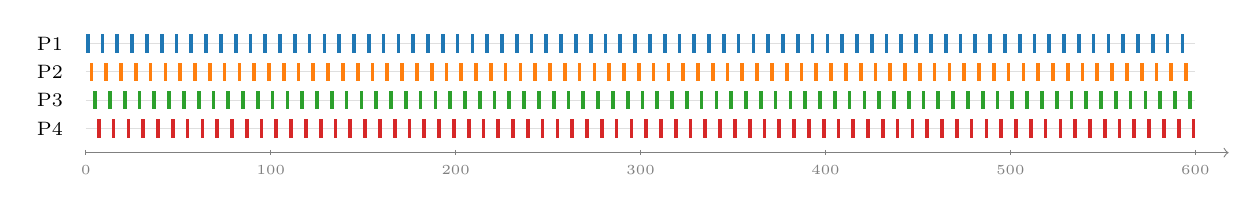
\begin{tikzpicture}[x=0.02349cm,y=0.36cm]
\node[anchor=east,font=\scriptsize] at (-7.2,3) {P1};
\draw[gray!25] (0,3) -- (600,3);
\node[anchor=east,font=\scriptsize] at (-7.2,2) {P2};
\draw[gray!25] (0,2) -- (600,2);
\node[anchor=east,font=\scriptsize] at (-7.2,1) {P3};
\draw[gray!25] (0,1) -- (600,1);
\node[anchor=east,font=\scriptsize] at (-7.2,0) {P4};
\draw[gray!25] (0,0) -- (600,0);
\fill[cP1] (0,2.68) rectangle (2,3.32);
\fill[cP2] (2,1.68) rectangle (4,2.32);
\fill[cP3] (4,0.68) rectangle (6,1.32);
\fill[cP4] (6,-0.32) rectangle (8,0.32);
\fill[cP1] (8,2.68) rectangle (10,3.32);
\fill[cP2] (10,1.68) rectangle (12,2.32);
\fill[cP3] (12,0.68) rectangle (14,1.32);
\fill[cP4] (14,-0.32) rectangle (16,0.32);
\fill[cP1] (16,2.68) rectangle (18,3.32);
\fill[cP2] (18,1.68) rectangle (20,2.32);
\fill[cP3] (20,0.68) rectangle (22,1.32);
\fill[cP4] (22,-0.32) rectangle (24,0.32);
\fill[cP1] (24,2.68) rectangle (26,3.32);
\fill[cP2] (26,1.68) rectangle (28,2.32);
\fill[cP3] (28,0.68) rectangle (30,1.32);
\fill[cP4] (30,-0.32) rectangle (32,0.32);
\fill[cP1] (32,2.68) rectangle (34,3.32);
\fill[cP2] (34,1.68) rectangle (36,2.32);
\fill[cP3] (36,0.68) rectangle (38,1.32);
\fill[cP4] (38,-0.32) rectangle (40,0.32);
\fill[cP1] (40,2.68) rectangle (42,3.32);
\fill[cP2] (42,1.68) rectangle (44,2.32);
\fill[cP3] (44,0.68) rectangle (46,1.32);
\fill[cP4] (46,-0.32) rectangle (48,0.32);
\fill[cP1] (48,2.68) rectangle (50,3.32);
\fill[cP2] (50,1.68) rectangle (52,2.32);
\fill[cP3] (52,0.68) rectangle (54,1.32);
\fill[cP4] (54,-0.32) rectangle (56,0.32);
\fill[cP1] (56,2.68) rectangle (58,3.32);
\fill[cP2] (58,1.68) rectangle (60,2.32);
\fill[cP3] (60,0.68) rectangle (62,1.32);
\fill[cP4] (62,-0.32) rectangle (64,0.32);
\fill[cP1] (64,2.68) rectangle (66,3.32);
\fill[cP2] (66,1.68) rectangle (68,2.32);
\fill[cP3] (68,0.68) rectangle (70,1.32);
\fill[cP4] (70,-0.32) rectangle (72,0.32);
\fill[cP1] (72,2.68) rectangle (74,3.32);
\fill[cP2] (74,1.68) rectangle (76,2.32);
\fill[cP3] (76,0.68) rectangle (78,1.32);
\fill[cP4] (78,-0.32) rectangle (80,0.32);
\fill[cP1] (80,2.68) rectangle (82,3.32);
\fill[cP2] (82,1.68) rectangle (84,2.32);
\fill[cP3] (84,0.68) rectangle (86,1.32);
\fill[cP4] (86,-0.32) rectangle (88,0.32);
\fill[cP1] (88,2.68) rectangle (90,3.32);
\fill[cP2] (90,1.68) rectangle (92,2.32);
\fill[cP3] (92,0.68) rectangle (94,1.32);
\fill[cP4] (94,-0.32) rectangle (96,0.32);
\fill[cP1] (96,2.68) rectangle (98,3.32);
\fill[cP2] (98,1.68) rectangle (100,2.32);
\fill[cP3] (100,0.68) rectangle (102,1.32);
\fill[cP4] (102,-0.32) rectangle (104,0.32);
\fill[cP1] (104,2.68) rectangle (106,3.32);
\fill[cP2] (106,1.68) rectangle (108,2.32);
\fill[cP3] (108,0.68) rectangle (110,1.32);
\fill[cP4] (110,-0.32) rectangle (112,0.32);
\fill[cP1] (112,2.68) rectangle (114,3.32);
\fill[cP2] (114,1.68) rectangle (116,2.32);
\fill[cP3] (116,0.68) rectangle (118,1.32);
\fill[cP4] (118,-0.32) rectangle (120,0.32);
\fill[cP1] (120,2.68) rectangle (122,3.32);
\fill[cP2] (122,1.68) rectangle (124,2.32);
\fill[cP3] (124,0.68) rectangle (126,1.32);
\fill[cP4] (126,-0.32) rectangle (128,0.32);
\fill[cP1] (128,2.68) rectangle (130,3.32);
\fill[cP2] (130,1.68) rectangle (132,2.32);
\fill[cP3] (132,0.68) rectangle (134,1.32);
\fill[cP4] (134,-0.32) rectangle (136,0.32);
\fill[cP1] (136,2.68) rectangle (138,3.32);
\fill[cP2] (138,1.68) rectangle (140,2.32);
\fill[cP3] (140,0.68) rectangle (142,1.32);
\fill[cP4] (142,-0.32) rectangle (144,0.32);
\fill[cP1] (144,2.68) rectangle (146,3.32);
\fill[cP2] (146,1.68) rectangle (148,2.32);
\fill[cP3] (148,0.68) rectangle (150,1.32);
\fill[cP4] (150,-0.32) rectangle (152,0.32);
\fill[cP1] (152,2.68) rectangle (154,3.32);
\fill[cP2] (154,1.68) rectangle (156,2.32);
\fill[cP3] (156,0.68) rectangle (158,1.32);
\fill[cP4] (158,-0.32) rectangle (160,0.32);
\fill[cP1] (160,2.68) rectangle (162,3.32);
\fill[cP2] (162,1.68) rectangle (164,2.32);
\fill[cP3] (164,0.68) rectangle (166,1.32);
\fill[cP4] (166,-0.32) rectangle (168,0.32);
\fill[cP1] (168,2.68) rectangle (170,3.32);
\fill[cP2] (170,1.68) rectangle (172,2.32);
\fill[cP3] (172,0.68) rectangle (174,1.32);
\fill[cP4] (174,-0.32) rectangle (176,0.32);
\fill[cP1] (176,2.68) rectangle (178,3.32);
\fill[cP2] (178,1.68) rectangle (180,2.32);
\fill[cP3] (180,0.68) rectangle (182,1.32);
\fill[cP4] (182,-0.32) rectangle (184,0.32);
\fill[cP1] (184,2.68) rectangle (186,3.32);
\fill[cP2] (186,1.68) rectangle (188,2.32);
\fill[cP3] (188,0.68) rectangle (190,1.32);
\fill[cP4] (190,-0.32) rectangle (192,0.32);
\fill[cP1] (192,2.68) rectangle (194,3.32);
\fill[cP2] (194,1.68) rectangle (196,2.32);
\fill[cP3] (196,0.68) rectangle (198,1.32);
\fill[cP4] (198,-0.32) rectangle (200,0.32);
\fill[cP1] (200,2.68) rectangle (202,3.32);
\fill[cP2] (202,1.68) rectangle (204,2.32);
\fill[cP3] (204,0.68) rectangle (206,1.32);
\fill[cP4] (206,-0.32) rectangle (208,0.32);
\fill[cP1] (208,2.68) rectangle (210,3.32);
\fill[cP2] (210,1.68) rectangle (212,2.32);
\fill[cP3] (212,0.68) rectangle (214,1.32);
\fill[cP4] (214,-0.32) rectangle (216,0.32);
\fill[cP1] (216,2.68) rectangle (218,3.32);
\fill[cP2] (218,1.68) rectangle (220,2.32);
\fill[cP3] (220,0.68) rectangle (222,1.32);
\fill[cP4] (222,-0.32) rectangle (224,0.32);
\fill[cP1] (224,2.68) rectangle (226,3.32);
\fill[cP2] (226,1.68) rectangle (228,2.32);
\fill[cP3] (228,0.68) rectangle (230,1.32);
\fill[cP4] (230,-0.32) rectangle (232,0.32);
\fill[cP1] (232,2.68) rectangle (234,3.32);
\fill[cP2] (234,1.68) rectangle (236,2.32);
\fill[cP3] (236,0.68) rectangle (238,1.32);
\fill[cP4] (238,-0.32) rectangle (240,0.32);
\fill[cP1] (240,2.68) rectangle (242,3.32);
\fill[cP2] (242,1.68) rectangle (244,2.32);
\fill[cP3] (244,0.68) rectangle (246,1.32);
\fill[cP4] (246,-0.32) rectangle (248,0.32);
\fill[cP1] (248,2.68) rectangle (250,3.32);
\fill[cP2] (250,1.68) rectangle (252,2.32);
\fill[cP3] (252,0.68) rectangle (254,1.32);
\fill[cP4] (254,-0.32) rectangle (256,0.32);
\fill[cP1] (256,2.68) rectangle (258,3.32);
\fill[cP2] (258,1.68) rectangle (260,2.32);
\fill[cP3] (260,0.68) rectangle (262,1.32);
\fill[cP4] (262,-0.32) rectangle (264,0.32);
\fill[cP1] (264,2.68) rectangle (266,3.32);
\fill[cP2] (266,1.68) rectangle (268,2.32);
\fill[cP3] (268,0.68) rectangle (270,1.32);
\fill[cP4] (270,-0.32) rectangle (272,0.32);
\fill[cP1] (272,2.68) rectangle (274,3.32);
\fill[cP2] (274,1.68) rectangle (276,2.32);
\fill[cP3] (276,0.68) rectangle (278,1.32);
\fill[cP4] (278,-0.32) rectangle (280,0.32);
\fill[cP1] (280,2.68) rectangle (282,3.32);
\fill[cP2] (282,1.68) rectangle (284,2.32);
\fill[cP3] (284,0.68) rectangle (286,1.32);
\fill[cP4] (286,-0.32) rectangle (288,0.32);
\fill[cP1] (288,2.68) rectangle (290,3.32);
\fill[cP2] (290,1.68) rectangle (292,2.32);
\fill[cP3] (292,0.68) rectangle (294,1.32);
\fill[cP4] (294,-0.32) rectangle (296,0.32);
\fill[cP1] (296,2.68) rectangle (298,3.32);
\fill[cP2] (298,1.68) rectangle (300,2.32);
\fill[cP3] (300,0.68) rectangle (302,1.32);
\fill[cP4] (302,-0.32) rectangle (304,0.32);
\fill[cP1] (304,2.68) rectangle (306,3.32);
\fill[cP2] (306,1.68) rectangle (308,2.32);
\fill[cP3] (308,0.68) rectangle (310,1.32);
\fill[cP4] (310,-0.32) rectangle (312,0.32);
\fill[cP1] (312,2.68) rectangle (314,3.32);
\fill[cP2] (314,1.68) rectangle (316,2.32);
\fill[cP3] (316,0.68) rectangle (318,1.32);
\fill[cP4] (318,-0.32) rectangle (320,0.32);
\fill[cP1] (320,2.68) rectangle (322,3.32);
\fill[cP2] (322,1.68) rectangle (324,2.32);
\fill[cP3] (324,0.68) rectangle (326,1.32);
\fill[cP4] (326,-0.32) rectangle (328,0.32);
\fill[cP1] (328,2.68) rectangle (330,3.32);
\fill[cP2] (330,1.68) rectangle (332,2.32);
\fill[cP3] (332,0.68) rectangle (334,1.32);
\fill[cP4] (334,-0.32) rectangle (336,0.32);
\fill[cP1] (336,2.68) rectangle (338,3.32);
\fill[cP2] (338,1.68) rectangle (340,2.32);
\fill[cP3] (340,0.68) rectangle (342,1.32);
\fill[cP4] (342,-0.32) rectangle (344,0.32);
\fill[cP1] (344,2.68) rectangle (346,3.32);
\fill[cP2] (346,1.68) rectangle (348,2.32);
\fill[cP3] (348,0.68) rectangle (350,1.32);
\fill[cP4] (350,-0.32) rectangle (352,0.32);
\fill[cP1] (352,2.68) rectangle (354,3.32);
\fill[cP2] (354,1.68) rectangle (356,2.32);
\fill[cP3] (356,0.68) rectangle (358,1.32);
\fill[cP4] (358,-0.32) rectangle (360,0.32);
\fill[cP1] (360,2.68) rectangle (362,3.32);
\fill[cP2] (362,1.68) rectangle (364,2.32);
\fill[cP3] (364,0.68) rectangle (366,1.32);
\fill[cP4] (366,-0.32) rectangle (368,0.32);
\fill[cP1] (368,2.68) rectangle (370,3.32);
\fill[cP2] (370,1.68) rectangle (372,2.32);
\fill[cP3] (372,0.68) rectangle (374,1.32);
\fill[cP4] (374,-0.32) rectangle (376,0.32);
\fill[cP1] (376,2.68) rectangle (378,3.32);
\fill[cP2] (378,1.68) rectangle (380,2.32);
\fill[cP3] (380,0.68) rectangle (382,1.32);
\fill[cP4] (382,-0.32) rectangle (384,0.32);
\fill[cP1] (384,2.68) rectangle (386,3.32);
\fill[cP2] (386,1.68) rectangle (388,2.32);
\fill[cP3] (388,0.68) rectangle (390,1.32);
\fill[cP4] (390,-0.32) rectangle (392,0.32);
\fill[cP1] (392,2.68) rectangle (394,3.32);
\fill[cP2] (394,1.68) rectangle (396,2.32);
\fill[cP3] (396,0.68) rectangle (398,1.32);
\fill[cP4] (398,-0.32) rectangle (400,0.32);
\fill[cP1] (400,2.68) rectangle (402,3.32);
\fill[cP2] (402,1.68) rectangle (404,2.32);
\fill[cP3] (404,0.68) rectangle (406,1.32);
\fill[cP4] (406,-0.32) rectangle (408,0.32);
\fill[cP1] (408,2.68) rectangle (410,3.32);
\fill[cP2] (410,1.68) rectangle (412,2.32);
\fill[cP3] (412,0.68) rectangle (414,1.32);
\fill[cP4] (414,-0.32) rectangle (416,0.32);
\fill[cP1] (416,2.68) rectangle (418,3.32);
\fill[cP2] (418,1.68) rectangle (420,2.32);
\fill[cP3] (420,0.68) rectangle (422,1.32);
\fill[cP4] (422,-0.32) rectangle (424,0.32);
\fill[cP1] (424,2.68) rectangle (426,3.32);
\fill[cP2] (426,1.68) rectangle (428,2.32);
\fill[cP3] (428,0.68) rectangle (430,1.32);
\fill[cP4] (430,-0.32) rectangle (432,0.32);
\fill[cP1] (432,2.68) rectangle (434,3.32);
\fill[cP2] (434,1.68) rectangle (436,2.32);
\fill[cP3] (436,0.68) rectangle (438,1.32);
\fill[cP4] (438,-0.32) rectangle (440,0.32);
\fill[cP1] (440,2.68) rectangle (442,3.32);
\fill[cP2] (442,1.68) rectangle (444,2.32);
\fill[cP3] (444,0.68) rectangle (446,1.32);
\fill[cP4] (446,-0.32) rectangle (448,0.32);
\fill[cP1] (448,2.68) rectangle (450,3.32);
\fill[cP2] (450,1.68) rectangle (452,2.32);
\fill[cP3] (452,0.68) rectangle (454,1.32);
\fill[cP4] (454,-0.32) rectangle (456,0.32);
\fill[cP1] (456,2.68) rectangle (458,3.32);
\fill[cP2] (458,1.68) rectangle (460,2.32);
\fill[cP3] (460,0.68) rectangle (462,1.32);
\fill[cP4] (462,-0.32) rectangle (464,0.32);
\fill[cP1] (464,2.68) rectangle (466,3.32);
\fill[cP2] (466,1.68) rectangle (468,2.32);
\fill[cP3] (468,0.68) rectangle (470,1.32);
\fill[cP4] (470,-0.32) rectangle (472,0.32);
\fill[cP1] (472,2.68) rectangle (474,3.32);
\fill[cP2] (474,1.68) rectangle (476,2.32);
\fill[cP3] (476,0.68) rectangle (478,1.32);
\fill[cP4] (478,-0.32) rectangle (480,0.32);
\fill[cP1] (480,2.68) rectangle (482,3.32);
\fill[cP2] (482,1.68) rectangle (484,2.32);
\fill[cP3] (484,0.68) rectangle (486,1.32);
\fill[cP4] (486,-0.32) rectangle (488,0.32);
\fill[cP1] (488,2.68) rectangle (490,3.32);
\fill[cP2] (490,1.68) rectangle (492,2.32);
\fill[cP3] (492,0.68) rectangle (494,1.32);
\fill[cP4] (494,-0.32) rectangle (496,0.32);
\fill[cP1] (496,2.68) rectangle (498,3.32);
\fill[cP2] (498,1.68) rectangle (500,2.32);
\fill[cP3] (500,0.68) rectangle (502,1.32);
\fill[cP4] (502,-0.32) rectangle (504,0.32);
\fill[cP1] (504,2.68) rectangle (506,3.32);
\fill[cP2] (506,1.68) rectangle (508,2.32);
\fill[cP3] (508,0.68) rectangle (510,1.32);
\fill[cP4] (510,-0.32) rectangle (512,0.32);
\fill[cP1] (512,2.68) rectangle (514,3.32);
\fill[cP2] (514,1.68) rectangle (516,2.32);
\fill[cP3] (516,0.68) rectangle (518,1.32);
\fill[cP4] (518,-0.32) rectangle (520,0.32);
\fill[cP1] (520,2.68) rectangle (522,3.32);
\fill[cP2] (522,1.68) rectangle (524,2.32);
\fill[cP3] (524,0.68) rectangle (526,1.32);
\fill[cP4] (526,-0.32) rectangle (528,0.32);
\fill[cP1] (528,2.68) rectangle (530,3.32);
\fill[cP2] (530,1.68) rectangle (532,2.32);
\fill[cP3] (532,0.68) rectangle (534,1.32);
\fill[cP4] (534,-0.32) rectangle (536,0.32);
\fill[cP1] (536,2.68) rectangle (538,3.32);
\fill[cP2] (538,1.68) rectangle (540,2.32);
\fill[cP3] (540,0.68) rectangle (542,1.32);
\fill[cP4] (542,-0.32) rectangle (544,0.32);
\fill[cP1] (544,2.68) rectangle (546,3.32);
\fill[cP2] (546,1.68) rectangle (548,2.32);
\fill[cP3] (548,0.68) rectangle (550,1.32);
\fill[cP4] (550,-0.32) rectangle (552,0.32);
\fill[cP1] (552,2.68) rectangle (554,3.32);
\fill[cP2] (554,1.68) rectangle (556,2.32);
\fill[cP3] (556,0.68) rectangle (558,1.32);
\fill[cP4] (558,-0.32) rectangle (560,0.32);
\fill[cP1] (560,2.68) rectangle (562,3.32);
\fill[cP2] (562,1.68) rectangle (564,2.32);
\fill[cP3] (564,0.68) rectangle (566,1.32);
\fill[cP4] (566,-0.32) rectangle (568,0.32);
\fill[cP1] (568,2.68) rectangle (570,3.32);
\fill[cP2] (570,1.68) rectangle (572,2.32);
\fill[cP3] (572,0.68) rectangle (574,1.32);
\fill[cP4] (574,-0.32) rectangle (576,0.32);
\fill[cP1] (576,2.68) rectangle (578,3.32);
\fill[cP2] (578,1.68) rectangle (580,2.32);
\fill[cP3] (580,0.68) rectangle (582,1.32);
\fill[cP4] (582,-0.32) rectangle (584,0.32);
\fill[cP1] (584,2.68) rectangle (586,3.32);
\fill[cP2] (586,1.68) rectangle (588,2.32);
\fill[cP3] (588,0.68) rectangle (590,1.32);
\fill[cP4] (590,-0.32) rectangle (592,0.32);
\fill[cP1] (592,2.68) rectangle (594,3.32);
\fill[cP2] (594,1.68) rectangle (596,2.32);
\fill[cP3] (596,0.68) rectangle (598,1.32);
\fill[cP4] (598,-0.32) rectangle (600,0.32);
\draw[->,gray] (0,-0.85) -- (618.0,-0.85);
\draw[gray] (0,-0.75)--(0,-0.95) node[below,font=\tiny]{0};
\draw[gray] (100,-0.75)--(100,-0.95) node[below,font=\tiny]{100};
\draw[gray] (200,-0.75)--(200,-0.95) node[below,font=\tiny]{200};
\draw[gray] (300,-0.75)--(300,-0.95) node[below,font=\tiny]{300};
\draw[gray] (400,-0.75)--(400,-0.95) node[below,font=\tiny]{400};
\draw[gray] (500,-0.75)--(500,-0.95) node[below,font=\tiny]{500};
\draw[gray] (600,-0.75)--(600,-0.95) node[below,font=\tiny]{600};
\end{tikzpicture}\par
\caption{Workload 2, single processor. The short 5-unit I/O bursts are almost entirely hidden behind other processes' computation, so all four policies keep the CPU busy for the full 600 units.}
\label{fig:gantt-single-2}
\end{figure}
\begin{figure}[H]\centering
\par\vspace{1.5mm}{\small\textbf{FIFO}\quad(makespan 16, idle 4)}\par\vspace{0.8mm}
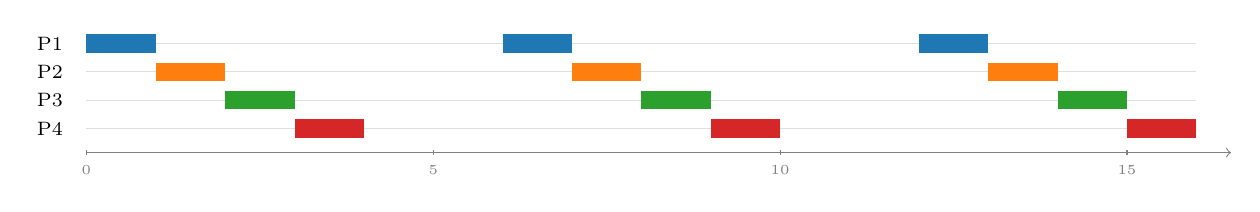
\begin{tikzpicture}[x=0.88095cm,y=0.36cm]
\node[anchor=east,font=\scriptsize] at (-0.2,3) {P1};
\draw[gray!25] (0,3) -- (16,3);
\node[anchor=east,font=\scriptsize] at (-0.2,2) {P2};
\draw[gray!25] (0,2) -- (16,2);
\node[anchor=east,font=\scriptsize] at (-0.2,1) {P3};
\draw[gray!25] (0,1) -- (16,1);
\node[anchor=east,font=\scriptsize] at (-0.2,0) {P4};
\draw[gray!25] (0,0) -- (16,0);
\fill[cP1] (0,2.68) rectangle (1,3.32);
\fill[cP2] (1,1.68) rectangle (2,2.32);
\fill[cP3] (2,0.68) rectangle (3,1.32);
\fill[cP4] (3,-0.32) rectangle (4,0.32);
\fill[cP1] (6,2.68) rectangle (7,3.32);
\fill[cP2] (7,1.68) rectangle (8,2.32);
\fill[cP3] (8,0.68) rectangle (9,1.32);
\fill[cP4] (9,-0.32) rectangle (10,0.32);
\fill[cP1] (12,2.68) rectangle (13,3.32);
\fill[cP2] (13,1.68) rectangle (14,2.32);
\fill[cP3] (14,0.68) rectangle (15,1.32);
\fill[cP4] (15,-0.32) rectangle (16,0.32);
\draw[->,gray] (0,-0.85) -- (16.5,-0.85);
\draw[gray] (0,-0.75)--(0,-0.95) node[below,font=\tiny]{0};
\draw[gray] (5,-0.75)--(5,-0.95) node[below,font=\tiny]{5};
\draw[gray] (10,-0.75)--(10,-0.95) node[below,font=\tiny]{10};
\draw[gray] (15,-0.75)--(15,-0.95) node[below,font=\tiny]{15};
\end{tikzpicture}\par
\par\vspace{1.5mm}{\small\textbf{RR}\quad(makespan 16, idle 4)}\par\vspace{0.8mm}
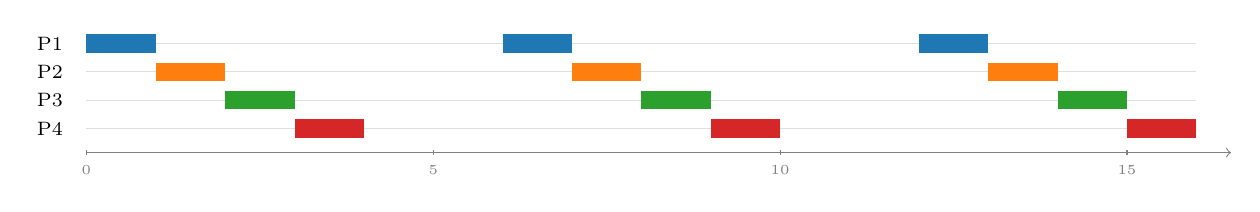
\begin{tikzpicture}[x=0.88095cm,y=0.36cm]
\node[anchor=east,font=\scriptsize] at (-0.2,3) {P1};
\draw[gray!25] (0,3) -- (16,3);
\node[anchor=east,font=\scriptsize] at (-0.2,2) {P2};
\draw[gray!25] (0,2) -- (16,2);
\node[anchor=east,font=\scriptsize] at (-0.2,1) {P3};
\draw[gray!25] (0,1) -- (16,1);
\node[anchor=east,font=\scriptsize] at (-0.2,0) {P4};
\draw[gray!25] (0,0) -- (16,0);
\fill[cP1] (0,2.68) rectangle (1,3.32);
\fill[cP2] (1,1.68) rectangle (2,2.32);
\fill[cP3] (2,0.68) rectangle (3,1.32);
\fill[cP4] (3,-0.32) rectangle (4,0.32);
\fill[cP1] (6,2.68) rectangle (7,3.32);
\fill[cP2] (7,1.68) rectangle (8,2.32);
\fill[cP3] (8,0.68) rectangle (9,1.32);
\fill[cP4] (9,-0.32) rectangle (10,0.32);
\fill[cP1] (12,2.68) rectangle (13,3.32);
\fill[cP2] (13,1.68) rectangle (14,2.32);
\fill[cP3] (14,0.68) rectangle (15,1.32);
\fill[cP4] (15,-0.32) rectangle (16,0.32);
\draw[->,gray] (0,-0.85) -- (16.5,-0.85);
\draw[gray] (0,-0.75)--(0,-0.95) node[below,font=\tiny]{0};
\draw[gray] (5,-0.75)--(5,-0.95) node[below,font=\tiny]{5};
\draw[gray] (10,-0.75)--(10,-0.95) node[below,font=\tiny]{10};
\draw[gray] (15,-0.75)--(15,-0.95) node[below,font=\tiny]{15};
\end{tikzpicture}\par
\par\vspace{1.5mm}{\small\textbf{MLFQ-NB}\quad(makespan 16, idle 4)}\par\vspace{0.8mm}
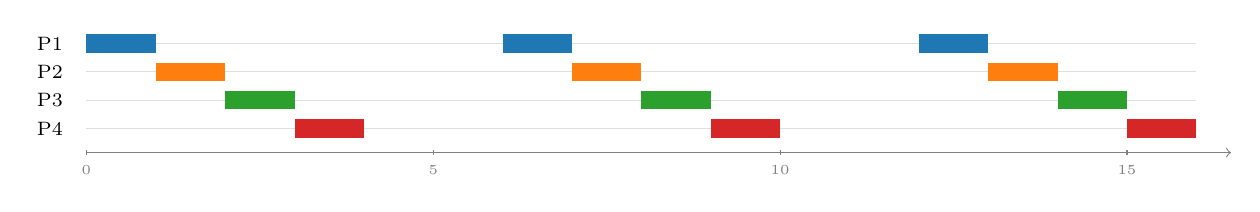
\begin{tikzpicture}[x=0.88095cm,y=0.36cm]
\node[anchor=east,font=\scriptsize] at (-0.2,3) {P1};
\draw[gray!25] (0,3) -- (16,3);
\node[anchor=east,font=\scriptsize] at (-0.2,2) {P2};
\draw[gray!25] (0,2) -- (16,2);
\node[anchor=east,font=\scriptsize] at (-0.2,1) {P3};
\draw[gray!25] (0,1) -- (16,1);
\node[anchor=east,font=\scriptsize] at (-0.2,0) {P4};
\draw[gray!25] (0,0) -- (16,0);
\fill[cP1] (0,2.68) rectangle (1,3.32);
\fill[cP2] (1,1.68) rectangle (2,2.32);
\fill[cP3] (2,0.68) rectangle (3,1.32);
\fill[cP4] (3,-0.32) rectangle (4,0.32);
\fill[cP1] (6,2.68) rectangle (7,3.32);
\fill[cP2] (7,1.68) rectangle (8,2.32);
\fill[cP3] (8,0.68) rectangle (9,1.32);
\fill[cP4] (9,-0.32) rectangle (10,0.32);
\fill[cP1] (12,2.68) rectangle (13,3.32);
\fill[cP2] (13,1.68) rectangle (14,2.32);
\fill[cP3] (14,0.68) rectangle (15,1.32);
\fill[cP4] (15,-0.32) rectangle (16,0.32);
\draw[->,gray] (0,-0.85) -- (16.5,-0.85);
\draw[gray] (0,-0.75)--(0,-0.95) node[below,font=\tiny]{0};
\draw[gray] (5,-0.75)--(5,-0.95) node[below,font=\tiny]{5};
\draw[gray] (10,-0.75)--(10,-0.95) node[below,font=\tiny]{10};
\draw[gray] (15,-0.75)--(15,-0.95) node[below,font=\tiny]{15};
\end{tikzpicture}\par
\par\vspace{1.5mm}{\small\textbf{MLFQ-WB}\quad(makespan 16, idle 4)}\par\vspace{0.8mm}
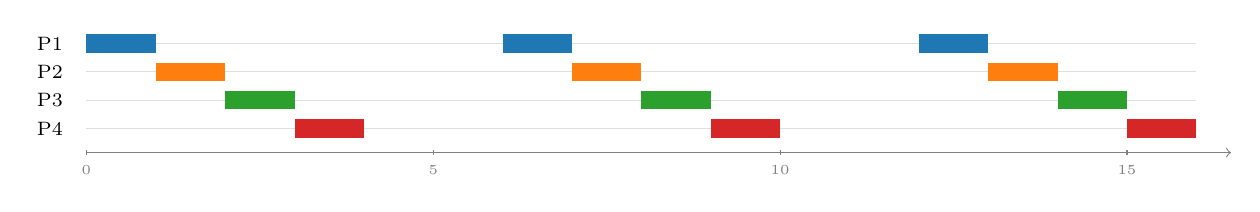
\begin{tikzpicture}[x=0.88095cm,y=0.36cm]
\node[anchor=east,font=\scriptsize] at (-0.2,3) {P1};
\draw[gray!25] (0,3) -- (16,3);
\node[anchor=east,font=\scriptsize] at (-0.2,2) {P2};
\draw[gray!25] (0,2) -- (16,2);
\node[anchor=east,font=\scriptsize] at (-0.2,1) {P3};
\draw[gray!25] (0,1) -- (16,1);
\node[anchor=east,font=\scriptsize] at (-0.2,0) {P4};
\draw[gray!25] (0,0) -- (16,0);
\fill[cP1] (0,2.68) rectangle (1,3.32);
\fill[cP2] (1,1.68) rectangle (2,2.32);
\fill[cP3] (2,0.68) rectangle (3,1.32);
\fill[cP4] (3,-0.32) rectangle (4,0.32);
\fill[cP1] (6,2.68) rectangle (7,3.32);
\fill[cP2] (7,1.68) rectangle (8,2.32);
\fill[cP3] (8,0.68) rectangle (9,1.32);
\fill[cP4] (9,-0.32) rectangle (10,0.32);
\fill[cP1] (12,2.68) rectangle (13,3.32);
\fill[cP2] (13,1.68) rectangle (14,2.32);
\fill[cP3] (14,0.68) rectangle (15,1.32);
\fill[cP4] (15,-0.32) rectangle (16,0.32);
\draw[->,gray] (0,-0.85) -- (16.5,-0.85);
\draw[gray] (0,-0.75)--(0,-0.95) node[below,font=\tiny]{0};
\draw[gray] (5,-0.75)--(5,-0.95) node[below,font=\tiny]{5};
\draw[gray] (10,-0.75)--(10,-0.95) node[below,font=\tiny]{10};
\draw[gray] (15,-0.75)--(15,-0.95) node[below,font=\tiny]{15};
\end{tikzpicture}\par
\caption{Workload 3, single processor. Every CPU burst is 1 unit, shorter than the quantum of 2, so preemption never triggers and all four schedules are identical. The CPU is idle in 2 gaps of 2 units (4 units in total), when every process is simultaneously blocked on I/O.}
\label{fig:gantt-single-3}
\end{figure}
\begin{figure}[H]\centering
\par\vspace{1.5mm}{\small\textbf{FIFO}\quad(makespan 178, idle 28)}\par\vspace{0.8mm}
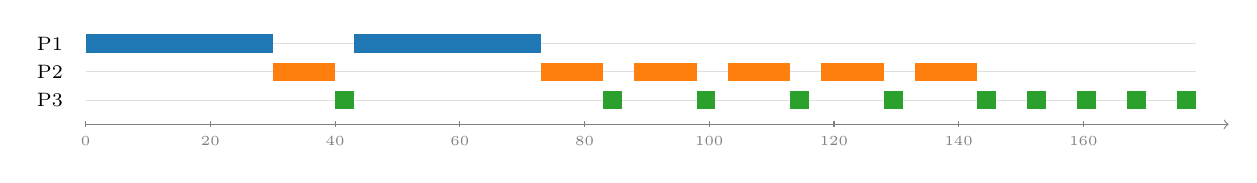
\begin{tikzpicture}[x=0.07919cm,y=0.36cm]
\node[anchor=east,font=\scriptsize] at (-2.1,2) {P1};
\draw[gray!25] (0,2) -- (178,2);
\node[anchor=east,font=\scriptsize] at (-2.1,1) {P2};
\draw[gray!25] (0,1) -- (178,1);
\node[anchor=east,font=\scriptsize] at (-2.1,0) {P3};
\draw[gray!25] (0,0) -- (178,0);
\fill[cP1] (0,1.68) rectangle (30,2.32);
\fill[cP2] (30,0.68) rectangle (40,1.32);
\fill[cP3] (40,-0.32) rectangle (43,0.32);
\fill[cP1] (43,1.68) rectangle (73,2.32);
\fill[cP2] (73,0.68) rectangle (83,1.32);
\fill[cP3] (83,-0.32) rectangle (86,0.32);
\fill[cP2] (88,0.68) rectangle (98,1.32);
\fill[cP3] (98,-0.32) rectangle (101,0.32);
\fill[cP2] (103,0.68) rectangle (113,1.32);
\fill[cP3] (113,-0.32) rectangle (116,0.32);
\fill[cP2] (118,0.68) rectangle (128,1.32);
\fill[cP3] (128,-0.32) rectangle (131,0.32);
\fill[cP2] (133,0.68) rectangle (143,1.32);
\fill[cP3] (143,-0.32) rectangle (146,0.32);
\fill[cP3] (151,-0.32) rectangle (154,0.32);
\fill[cP3] (159,-0.32) rectangle (162,0.32);
\fill[cP3] (167,-0.32) rectangle (170,0.32);
\fill[cP3] (175,-0.32) rectangle (178,0.32);
\draw[->,gray] (0,-0.85) -- (183.3,-0.85);
\draw[gray] (0,-0.75)--(0,-0.95) node[below,font=\tiny]{0};
\draw[gray] (20,-0.75)--(20,-0.95) node[below,font=\tiny]{20};
\draw[gray] (40,-0.75)--(40,-0.95) node[below,font=\tiny]{40};
\draw[gray] (60,-0.75)--(60,-0.95) node[below,font=\tiny]{60};
\draw[gray] (80,-0.75)--(80,-0.95) node[below,font=\tiny]{80};
\draw[gray] (100,-0.75)--(100,-0.95) node[below,font=\tiny]{100};
\draw[gray] (120,-0.75)--(120,-0.95) node[below,font=\tiny]{120};
\draw[gray] (140,-0.75)--(140,-0.95) node[below,font=\tiny]{140};
\draw[gray] (160,-0.75)--(160,-0.95) node[below,font=\tiny]{160};
\end{tikzpicture}\par
\par\vspace{1.5mm}{\small\textbf{RR}\quad(makespan 152, idle 2)}\par\vspace{0.8mm}
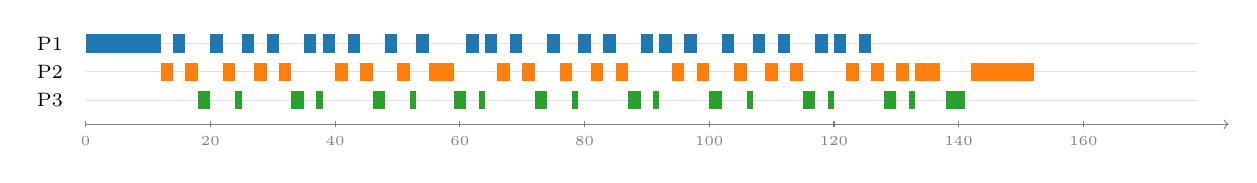
\begin{tikzpicture}[x=0.07919cm,y=0.36cm]
\node[anchor=east,font=\scriptsize] at (-2.1,2) {P1};
\draw[gray!25] (0,2) -- (178,2);
\node[anchor=east,font=\scriptsize] at (-2.1,1) {P2};
\draw[gray!25] (0,1) -- (178,1);
\node[anchor=east,font=\scriptsize] at (-2.1,0) {P3};
\draw[gray!25] (0,0) -- (178,0);
\fill[cP1] (0,1.68) rectangle (12,2.32);
\fill[cP2] (12,0.68) rectangle (14,1.32);
\fill[cP1] (14,1.68) rectangle (16,2.32);
\fill[cP2] (16,0.68) rectangle (18,1.32);
\fill[cP3] (18,-0.32) rectangle (20,0.32);
\fill[cP1] (20,1.68) rectangle (22,2.32);
\fill[cP2] (22,0.68) rectangle (24,1.32);
\fill[cP3] (24,-0.32) rectangle (25,0.32);
\fill[cP1] (25,1.68) rectangle (27,2.32);
\fill[cP2] (27,0.68) rectangle (29,1.32);
\fill[cP1] (29,1.68) rectangle (31,2.32);
\fill[cP2] (31,0.68) rectangle (33,1.32);
\fill[cP3] (33,-0.32) rectangle (35,0.32);
\fill[cP1] (35,1.68) rectangle (37,2.32);
\fill[cP3] (37,-0.32) rectangle (38,0.32);
\fill[cP1] (38,1.68) rectangle (40,2.32);
\fill[cP2] (40,0.68) rectangle (42,1.32);
\fill[cP1] (42,1.68) rectangle (44,2.32);
\fill[cP2] (44,0.68) rectangle (46,1.32);
\fill[cP3] (46,-0.32) rectangle (48,0.32);
\fill[cP1] (48,1.68) rectangle (50,2.32);
\fill[cP2] (50,0.68) rectangle (52,1.32);
\fill[cP3] (52,-0.32) rectangle (53,0.32);
\fill[cP1] (53,1.68) rectangle (55,2.32);
\fill[cP2] (55,0.68) rectangle (59,1.32);
\fill[cP3] (59,-0.32) rectangle (61,0.32);
\fill[cP1] (61,1.68) rectangle (63,2.32);
\fill[cP3] (63,-0.32) rectangle (64,0.32);
\fill[cP1] (64,1.68) rectangle (66,2.32);
\fill[cP2] (66,0.68) rectangle (68,1.32);
\fill[cP1] (68,1.68) rectangle (70,2.32);
\fill[cP2] (70,0.68) rectangle (72,1.32);
\fill[cP3] (72,-0.32) rectangle (74,0.32);
\fill[cP1] (74,1.68) rectangle (76,2.32);
\fill[cP2] (76,0.68) rectangle (78,1.32);
\fill[cP3] (78,-0.32) rectangle (79,0.32);
\fill[cP1] (79,1.68) rectangle (81,2.32);
\fill[cP2] (81,0.68) rectangle (83,1.32);
\fill[cP1] (83,1.68) rectangle (85,2.32);
\fill[cP2] (85,0.68) rectangle (87,1.32);
\fill[cP3] (87,-0.32) rectangle (89,0.32);
\fill[cP1] (89,1.68) rectangle (91,2.32);
\fill[cP3] (91,-0.32) rectangle (92,0.32);
\fill[cP1] (92,1.68) rectangle (94,2.32);
\fill[cP2] (94,0.68) rectangle (96,1.32);
\fill[cP1] (96,1.68) rectangle (98,2.32);
\fill[cP2] (98,0.68) rectangle (100,1.32);
\fill[cP3] (100,-0.32) rectangle (102,0.32);
\fill[cP1] (102,1.68) rectangle (104,2.32);
\fill[cP2] (104,0.68) rectangle (106,1.32);
\fill[cP3] (106,-0.32) rectangle (107,0.32);
\fill[cP1] (107,1.68) rectangle (109,2.32);
\fill[cP2] (109,0.68) rectangle (111,1.32);
\fill[cP1] (111,1.68) rectangle (113,2.32);
\fill[cP2] (113,0.68) rectangle (115,1.32);
\fill[cP3] (115,-0.32) rectangle (117,0.32);
\fill[cP1] (117,1.68) rectangle (119,2.32);
\fill[cP3] (119,-0.32) rectangle (120,0.32);
\fill[cP1] (120,1.68) rectangle (122,2.32);
\fill[cP2] (122,0.68) rectangle (124,1.32);
\fill[cP1] (124,1.68) rectangle (126,2.32);
\fill[cP2] (126,0.68) rectangle (128,1.32);
\fill[cP3] (128,-0.32) rectangle (130,0.32);
\fill[cP2] (130,0.68) rectangle (132,1.32);
\fill[cP3] (132,-0.32) rectangle (133,0.32);
\fill[cP2] (133,0.68) rectangle (137,1.32);
\fill[cP3] (138,-0.32) rectangle (141,0.32);
\fill[cP2] (142,0.68) rectangle (152,1.32);
\draw[->,gray] (0,-0.85) -- (183.3,-0.85);
\draw[gray] (0,-0.75)--(0,-0.95) node[below,font=\tiny]{0};
\draw[gray] (20,-0.75)--(20,-0.95) node[below,font=\tiny]{20};
\draw[gray] (40,-0.75)--(40,-0.95) node[below,font=\tiny]{40};
\draw[gray] (60,-0.75)--(60,-0.95) node[below,font=\tiny]{60};
\draw[gray] (80,-0.75)--(80,-0.95) node[below,font=\tiny]{80};
\draw[gray] (100,-0.75)--(100,-0.95) node[below,font=\tiny]{100};
\draw[gray] (120,-0.75)--(120,-0.95) node[below,font=\tiny]{120};
\draw[gray] (140,-0.75)--(140,-0.95) node[below,font=\tiny]{140};
\draw[gray] (160,-0.75)--(160,-0.95) node[below,font=\tiny]{160};
\end{tikzpicture}\par
\par\vspace{1.5mm}{\small\textbf{MLFQ-NB}\quad(makespan 154, idle 4)}\par\vspace{0.8mm}
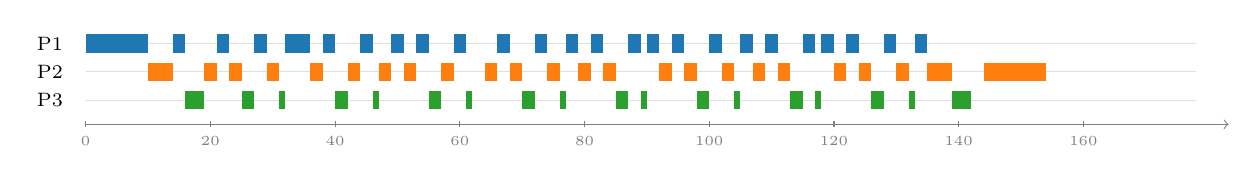
\begin{tikzpicture}[x=0.07919cm,y=0.36cm]
\node[anchor=east,font=\scriptsize] at (-2.1,2) {P1};
\draw[gray!25] (0,2) -- (178,2);
\node[anchor=east,font=\scriptsize] at (-2.1,1) {P2};
\draw[gray!25] (0,1) -- (178,1);
\node[anchor=east,font=\scriptsize] at (-2.1,0) {P3};
\draw[gray!25] (0,0) -- (178,0);
\fill[cP1] (0,1.68) rectangle (10,2.32);
\fill[cP2] (10,0.68) rectangle (14,1.32);
\fill[cP1] (14,1.68) rectangle (16,2.32);
\fill[cP3] (16,-0.32) rectangle (19,0.32);
\fill[cP2] (19,0.68) rectangle (21,1.32);
\fill[cP1] (21,1.68) rectangle (23,2.32);
\fill[cP2] (23,0.68) rectangle (25,1.32);
\fill[cP3] (25,-0.32) rectangle (27,0.32);
\fill[cP1] (27,1.68) rectangle (29,2.32);
\fill[cP2] (29,0.68) rectangle (31,1.32);
\fill[cP3] (31,-0.32) rectangle (32,0.32);
\fill[cP1] (32,1.68) rectangle (36,2.32);
\fill[cP2] (36,0.68) rectangle (38,1.32);
\fill[cP1] (38,1.68) rectangle (40,2.32);
\fill[cP3] (40,-0.32) rectangle (42,0.32);
\fill[cP2] (42,0.68) rectangle (44,1.32);
\fill[cP1] (44,1.68) rectangle (46,2.32);
\fill[cP3] (46,-0.32) rectangle (47,0.32);
\fill[cP2] (47,0.68) rectangle (49,1.32);
\fill[cP1] (49,1.68) rectangle (51,2.32);
\fill[cP2] (51,0.68) rectangle (53,1.32);
\fill[cP1] (53,1.68) rectangle (55,2.32);
\fill[cP3] (55,-0.32) rectangle (57,0.32);
\fill[cP2] (57,0.68) rectangle (59,1.32);
\fill[cP1] (59,1.68) rectangle (61,2.32);
\fill[cP3] (61,-0.32) rectangle (62,0.32);
\fill[cP2] (64,0.68) rectangle (66,1.32);
\fill[cP1] (66,1.68) rectangle (68,2.32);
\fill[cP2] (68,0.68) rectangle (70,1.32);
\fill[cP3] (70,-0.32) rectangle (72,0.32);
\fill[cP1] (72,1.68) rectangle (74,2.32);
\fill[cP2] (74,0.68) rectangle (76,1.32);
\fill[cP3] (76,-0.32) rectangle (77,0.32);
\fill[cP1] (77,1.68) rectangle (79,2.32);
\fill[cP2] (79,0.68) rectangle (81,1.32);
\fill[cP1] (81,1.68) rectangle (83,2.32);
\fill[cP2] (83,0.68) rectangle (85,1.32);
\fill[cP3] (85,-0.32) rectangle (87,0.32);
\fill[cP1] (87,1.68) rectangle (89,2.32);
\fill[cP3] (89,-0.32) rectangle (90,0.32);
\fill[cP1] (90,1.68) rectangle (92,2.32);
\fill[cP2] (92,0.68) rectangle (94,1.32);
\fill[cP1] (94,1.68) rectangle (96,2.32);
\fill[cP2] (96,0.68) rectangle (98,1.32);
\fill[cP3] (98,-0.32) rectangle (100,0.32);
\fill[cP1] (100,1.68) rectangle (102,2.32);
\fill[cP2] (102,0.68) rectangle (104,1.32);
\fill[cP3] (104,-0.32) rectangle (105,0.32);
\fill[cP1] (105,1.68) rectangle (107,2.32);
\fill[cP2] (107,0.68) rectangle (109,1.32);
\fill[cP1] (109,1.68) rectangle (111,2.32);
\fill[cP2] (111,0.68) rectangle (113,1.32);
\fill[cP3] (113,-0.32) rectangle (115,0.32);
\fill[cP1] (115,1.68) rectangle (117,2.32);
\fill[cP3] (117,-0.32) rectangle (118,0.32);
\fill[cP1] (118,1.68) rectangle (120,2.32);
\fill[cP2] (120,0.68) rectangle (122,1.32);
\fill[cP1] (122,1.68) rectangle (124,2.32);
\fill[cP2] (124,0.68) rectangle (126,1.32);
\fill[cP3] (126,-0.32) rectangle (128,0.32);
\fill[cP1] (128,1.68) rectangle (130,2.32);
\fill[cP2] (130,0.68) rectangle (132,1.32);
\fill[cP3] (132,-0.32) rectangle (133,0.32);
\fill[cP1] (133,1.68) rectangle (135,2.32);
\fill[cP2] (135,0.68) rectangle (139,1.32);
\fill[cP3] (139,-0.32) rectangle (142,0.32);
\fill[cP2] (144,0.68) rectangle (154,1.32);
\draw[->,gray] (0,-0.85) -- (183.3,-0.85);
\draw[gray] (0,-0.75)--(0,-0.95) node[below,font=\tiny]{0};
\draw[gray] (20,-0.75)--(20,-0.95) node[below,font=\tiny]{20};
\draw[gray] (40,-0.75)--(40,-0.95) node[below,font=\tiny]{40};
\draw[gray] (60,-0.75)--(60,-0.95) node[below,font=\tiny]{60};
\draw[gray] (80,-0.75)--(80,-0.95) node[below,font=\tiny]{80};
\draw[gray] (100,-0.75)--(100,-0.95) node[below,font=\tiny]{100};
\draw[gray] (120,-0.75)--(120,-0.95) node[below,font=\tiny]{120};
\draw[gray] (140,-0.75)--(140,-0.95) node[below,font=\tiny]{140};
\draw[gray] (160,-0.75)--(160,-0.95) node[below,font=\tiny]{160};
\end{tikzpicture}\par
\par\vspace{1.5mm}{\small\textbf{MLFQ-WB}\quad(makespan 157, idle 7)}\par\vspace{0.8mm}
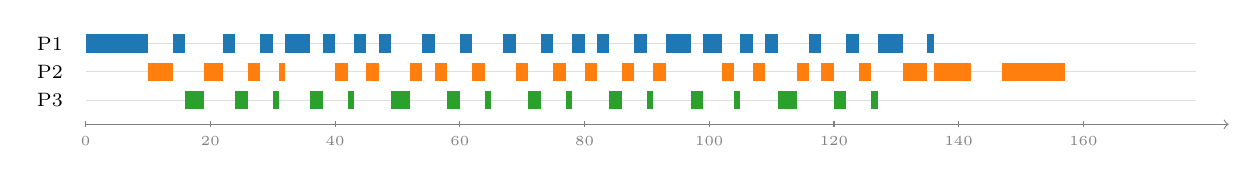
\begin{tikzpicture}[x=0.07919cm,y=0.36cm]
\node[anchor=east,font=\scriptsize] at (-2.1,2) {P1};
\draw[gray!25] (0,2) -- (178,2);
\node[anchor=east,font=\scriptsize] at (-2.1,1) {P2};
\draw[gray!25] (0,1) -- (178,1);
\node[anchor=east,font=\scriptsize] at (-2.1,0) {P3};
\draw[gray!25] (0,0) -- (178,0);
\fill[cP1] (0,1.68) rectangle (10,2.32);
\fill[cP2] (10,0.68) rectangle (14,1.32);
\fill[cP1] (14,1.68) rectangle (16,2.32);
\fill[cP3] (16,-0.32) rectangle (19,0.32);
\fill[cP2] (19,0.68) rectangle (22,1.32);
\fill[cP1] (22,1.68) rectangle (24,2.32);
\fill[cP3] (24,-0.32) rectangle (26,0.32);
\fill[cP2] (26,0.68) rectangle (28,1.32);
\fill[cP1] (28,1.68) rectangle (30,2.32);
\fill[cP3] (30,-0.32) rectangle (31,0.32);
\fill[cP2] (31,0.68) rectangle (32,1.32);
\fill[cP1] (32,1.68) rectangle (36,2.32);
\fill[cP3] (36,-0.32) rectangle (38,0.32);
\fill[cP1] (38,1.68) rectangle (40,2.32);
\fill[cP2] (40,0.68) rectangle (42,1.32);
\fill[cP3] (42,-0.32) rectangle (43,0.32);
\fill[cP1] (43,1.68) rectangle (45,2.32);
\fill[cP2] (45,0.68) rectangle (47,1.32);
\fill[cP1] (47,1.68) rectangle (49,2.32);
\fill[cP3] (49,-0.32) rectangle (52,0.32);
\fill[cP2] (52,0.68) rectangle (54,1.32);
\fill[cP1] (54,1.68) rectangle (56,2.32);
\fill[cP2] (56,0.68) rectangle (58,1.32);
\fill[cP3] (58,-0.32) rectangle (60,0.32);
\fill[cP1] (60,1.68) rectangle (62,2.32);
\fill[cP2] (62,0.68) rectangle (64,1.32);
\fill[cP3] (64,-0.32) rectangle (65,0.32);
\fill[cP1] (67,1.68) rectangle (69,2.32);
\fill[cP2] (69,0.68) rectangle (71,1.32);
\fill[cP3] (71,-0.32) rectangle (73,0.32);
\fill[cP1] (73,1.68) rectangle (75,2.32);
\fill[cP2] (75,0.68) rectangle (77,1.32);
\fill[cP3] (77,-0.32) rectangle (78,0.32);
\fill[cP1] (78,1.68) rectangle (80,2.32);
\fill[cP2] (80,0.68) rectangle (82,1.32);
\fill[cP1] (82,1.68) rectangle (84,2.32);
\fill[cP3] (84,-0.32) rectangle (86,0.32);
\fill[cP2] (86,0.68) rectangle (88,1.32);
\fill[cP1] (88,1.68) rectangle (90,2.32);
\fill[cP3] (90,-0.32) rectangle (91,0.32);
\fill[cP2] (91,0.68) rectangle (93,1.32);
\fill[cP1] (93,1.68) rectangle (97,2.32);
\fill[cP3] (97,-0.32) rectangle (99,0.32);
\fill[cP1] (99,1.68) rectangle (102,2.32);
\fill[cP2] (102,0.68) rectangle (104,1.32);
\fill[cP3] (104,-0.32) rectangle (105,0.32);
\fill[cP1] (105,1.68) rectangle (107,2.32);
\fill[cP2] (107,0.68) rectangle (109,1.32);
\fill[cP1] (109,1.68) rectangle (111,2.32);
\fill[cP3] (111,-0.32) rectangle (114,0.32);
\fill[cP2] (114,0.68) rectangle (116,1.32);
\fill[cP1] (116,1.68) rectangle (118,2.32);
\fill[cP2] (118,0.68) rectangle (120,1.32);
\fill[cP3] (120,-0.32) rectangle (122,0.32);
\fill[cP1] (122,1.68) rectangle (124,2.32);
\fill[cP2] (124,0.68) rectangle (126,1.32);
\fill[cP3] (126,-0.32) rectangle (127,0.32);
\fill[cP1] (127,1.68) rectangle (131,2.32);
\fill[cP2] (131,0.68) rectangle (135,1.32);
\fill[cP1] (135,1.68) rectangle (136,2.32);
\fill[cP2] (136,0.68) rectangle (142,1.32);
\fill[cP2] (147,0.68) rectangle (157,1.32);
\draw[->,gray] (0,-0.85) -- (183.3,-0.85);
\draw[gray] (0,-0.75)--(0,-0.95) node[below,font=\tiny]{0};
\draw[gray] (20,-0.75)--(20,-0.95) node[below,font=\tiny]{20};
\draw[gray] (40,-0.75)--(40,-0.95) node[below,font=\tiny]{40};
\draw[gray] (60,-0.75)--(60,-0.95) node[below,font=\tiny]{60};
\draw[gray] (80,-0.75)--(80,-0.95) node[below,font=\tiny]{80};
\draw[gray] (100,-0.75)--(100,-0.95) node[below,font=\tiny]{100};
\draw[gray] (120,-0.75)--(120,-0.95) node[below,font=\tiny]{120};
\draw[gray] (140,-0.75)--(140,-0.95) node[below,font=\tiny]{140};
\draw[gray] (160,-0.75)--(160,-0.95) node[below,font=\tiny]{160};
\end{tikzpicture}\par
\caption{Workload 4, single processor. FIFO (top) leaves the CPU idle for 28 time units and stretches P3's completion to 178; the preemptive policies interleave the three processes, cut idle time to 2--7 units and finish 21--26 time units earlier.}
\label{fig:gantt-single-4}
\end{figure}
\begin{figure}[H]\centering
\par\vspace{1.5mm}{\small\textbf{FIFO}\quad(makespan 240, idle 0)}\par\vspace{0.8mm}
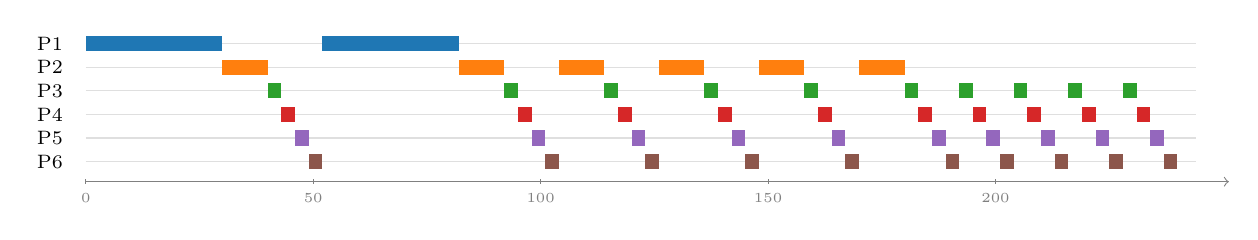
\begin{tikzpicture}[x=0.05777cm,y=0.30cm]
\node[anchor=east,font=\scriptsize] at (-2.9,5) {P1};
\draw[gray!25] (0,5) -- (244,5);
\node[anchor=east,font=\scriptsize] at (-2.9,4) {P2};
\draw[gray!25] (0,4) -- (244,4);
\node[anchor=east,font=\scriptsize] at (-2.9,3) {P3};
\draw[gray!25] (0,3) -- (244,3);
\node[anchor=east,font=\scriptsize] at (-2.9,2) {P4};
\draw[gray!25] (0,2) -- (244,2);
\node[anchor=east,font=\scriptsize] at (-2.9,1) {P5};
\draw[gray!25] (0,1) -- (244,1);
\node[anchor=east,font=\scriptsize] at (-2.9,0) {P6};
\draw[gray!25] (0,0) -- (244,0);
\fill[cP1] (0,4.68) rectangle (30,5.32);
\fill[cP2] (30,3.68) rectangle (40,4.32);
\fill[cP3] (40,2.68) rectangle (43,3.32);
\fill[cP4] (43,1.68) rectangle (46,2.32);
\fill[cP5] (46,0.68) rectangle (49,1.32);
\fill[cP6] (49,-0.32) rectangle (52,0.32);
\fill[cP1] (52,4.68) rectangle (82,5.32);
\fill[cP2] (82,3.68) rectangle (92,4.32);
\fill[cP3] (92,2.68) rectangle (95,3.32);
\fill[cP4] (95,1.68) rectangle (98,2.32);
\fill[cP5] (98,0.68) rectangle (101,1.32);
\fill[cP6] (101,-0.32) rectangle (104,0.32);
\fill[cP2] (104,3.68) rectangle (114,4.32);
\fill[cP3] (114,2.68) rectangle (117,3.32);
\fill[cP4] (117,1.68) rectangle (120,2.32);
\fill[cP5] (120,0.68) rectangle (123,1.32);
\fill[cP6] (123,-0.32) rectangle (126,0.32);
\fill[cP2] (126,3.68) rectangle (136,4.32);
\fill[cP3] (136,2.68) rectangle (139,3.32);
\fill[cP4] (139,1.68) rectangle (142,2.32);
\fill[cP5] (142,0.68) rectangle (145,1.32);
\fill[cP6] (145,-0.32) rectangle (148,0.32);
\fill[cP2] (148,3.68) rectangle (158,4.32);
\fill[cP3] (158,2.68) rectangle (161,3.32);
\fill[cP4] (161,1.68) rectangle (164,2.32);
\fill[cP5] (164,0.68) rectangle (167,1.32);
\fill[cP6] (167,-0.32) rectangle (170,0.32);
\fill[cP2] (170,3.68) rectangle (180,4.32);
\fill[cP3] (180,2.68) rectangle (183,3.32);
\fill[cP4] (183,1.68) rectangle (186,2.32);
\fill[cP5] (186,0.68) rectangle (189,1.32);
\fill[cP6] (189,-0.32) rectangle (192,0.32);
\fill[cP3] (192,2.68) rectangle (195,3.32);
\fill[cP4] (195,1.68) rectangle (198,2.32);
\fill[cP5] (198,0.68) rectangle (201,1.32);
\fill[cP6] (201,-0.32) rectangle (204,0.32);
\fill[cP3] (204,2.68) rectangle (207,3.32);
\fill[cP4] (207,1.68) rectangle (210,2.32);
\fill[cP5] (210,0.68) rectangle (213,1.32);
\fill[cP6] (213,-0.32) rectangle (216,0.32);
\fill[cP3] (216,2.68) rectangle (219,3.32);
\fill[cP4] (219,1.68) rectangle (222,2.32);
\fill[cP5] (222,0.68) rectangle (225,1.32);
\fill[cP6] (225,-0.32) rectangle (228,0.32);
\fill[cP3] (228,2.68) rectangle (231,3.32);
\fill[cP4] (231,1.68) rectangle (234,2.32);
\fill[cP5] (234,0.68) rectangle (237,1.32);
\fill[cP6] (237,-0.32) rectangle (240,0.32);
\draw[->,gray] (0,-0.85) -- (251.3,-0.85);
\draw[gray] (0,-0.75)--(0,-0.95) node[below,font=\tiny]{0};
\draw[gray] (50,-0.75)--(50,-0.95) node[below,font=\tiny]{50};
\draw[gray] (100,-0.75)--(100,-0.95) node[below,font=\tiny]{100};
\draw[gray] (150,-0.75)--(150,-0.95) node[below,font=\tiny]{150};
\draw[gray] (200,-0.75)--(200,-0.95) node[below,font=\tiny]{200};
\end{tikzpicture}\par
\par\vspace{1.5mm}{\small\textbf{RR}\quad(makespan 244, idle 4)}\par\vspace{0.8mm}
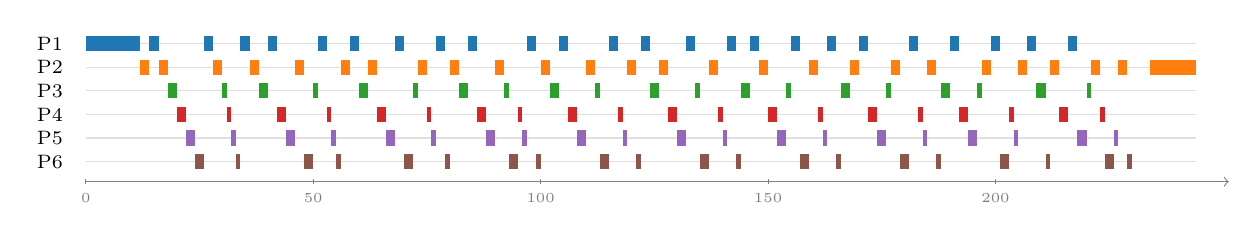
\begin{tikzpicture}[x=0.05777cm,y=0.30cm]
\node[anchor=east,font=\scriptsize] at (-2.9,5) {P1};
\draw[gray!25] (0,5) -- (244,5);
\node[anchor=east,font=\scriptsize] at (-2.9,4) {P2};
\draw[gray!25] (0,4) -- (244,4);
\node[anchor=east,font=\scriptsize] at (-2.9,3) {P3};
\draw[gray!25] (0,3) -- (244,3);
\node[anchor=east,font=\scriptsize] at (-2.9,2) {P4};
\draw[gray!25] (0,2) -- (244,2);
\node[anchor=east,font=\scriptsize] at (-2.9,1) {P5};
\draw[gray!25] (0,1) -- (244,1);
\node[anchor=east,font=\scriptsize] at (-2.9,0) {P6};
\draw[gray!25] (0,0) -- (244,0);
\fill[cP1] (0,4.68) rectangle (12,5.32);
\fill[cP2] (12,3.68) rectangle (14,4.32);
\fill[cP1] (14,4.68) rectangle (16,5.32);
\fill[cP2] (16,3.68) rectangle (18,4.32);
\fill[cP3] (18,2.68) rectangle (20,3.32);
\fill[cP4] (20,1.68) rectangle (22,2.32);
\fill[cP5] (22,0.68) rectangle (24,1.32);
\fill[cP6] (24,-0.32) rectangle (26,0.32);
\fill[cP1] (26,4.68) rectangle (28,5.32);
\fill[cP2] (28,3.68) rectangle (30,4.32);
\fill[cP3] (30,2.68) rectangle (31,3.32);
\fill[cP4] (31,1.68) rectangle (32,2.32);
\fill[cP5] (32,0.68) rectangle (33,1.32);
\fill[cP6] (33,-0.32) rectangle (34,0.32);
\fill[cP1] (34,4.68) rectangle (36,5.32);
\fill[cP2] (36,3.68) rectangle (38,4.32);
\fill[cP3] (38,2.68) rectangle (40,3.32);
\fill[cP1] (40,4.68) rectangle (42,5.32);
\fill[cP4] (42,1.68) rectangle (44,2.32);
\fill[cP5] (44,0.68) rectangle (46,1.32);
\fill[cP2] (46,3.68) rectangle (48,4.32);
\fill[cP6] (48,-0.32) rectangle (50,0.32);
\fill[cP3] (50,2.68) rectangle (51,3.32);
\fill[cP1] (51,4.68) rectangle (53,5.32);
\fill[cP4] (53,1.68) rectangle (54,2.32);
\fill[cP5] (54,0.68) rectangle (55,1.32);
\fill[cP6] (55,-0.32) rectangle (56,0.32);
\fill[cP2] (56,3.68) rectangle (58,4.32);
\fill[cP1] (58,4.68) rectangle (60,5.32);
\fill[cP3] (60,2.68) rectangle (62,3.32);
\fill[cP2] (62,3.68) rectangle (64,4.32);
\fill[cP4] (64,1.68) rectangle (66,2.32);
\fill[cP5] (66,0.68) rectangle (68,1.32);
\fill[cP1] (68,4.68) rectangle (70,5.32);
\fill[cP6] (70,-0.32) rectangle (72,0.32);
\fill[cP3] (72,2.68) rectangle (73,3.32);
\fill[cP2] (73,3.68) rectangle (75,4.32);
\fill[cP4] (75,1.68) rectangle (76,2.32);
\fill[cP5] (76,0.68) rectangle (77,1.32);
\fill[cP1] (77,4.68) rectangle (79,5.32);
\fill[cP6] (79,-0.32) rectangle (80,0.32);
\fill[cP2] (80,3.68) rectangle (82,4.32);
\fill[cP3] (82,2.68) rectangle (84,3.32);
\fill[cP1] (84,4.68) rectangle (86,5.32);
\fill[cP4] (86,1.68) rectangle (88,2.32);
\fill[cP5] (88,0.68) rectangle (90,1.32);
\fill[cP2] (90,3.68) rectangle (92,4.32);
\fill[cP3] (92,2.68) rectangle (93,3.32);
\fill[cP6] (93,-0.32) rectangle (95,0.32);
\fill[cP4] (95,1.68) rectangle (96,2.32);
\fill[cP5] (96,0.68) rectangle (97,1.32);
\fill[cP1] (97,4.68) rectangle (99,5.32);
\fill[cP6] (99,-0.32) rectangle (100,0.32);
\fill[cP2] (100,3.68) rectangle (102,4.32);
\fill[cP3] (102,2.68) rectangle (104,3.32);
\fill[cP1] (104,4.68) rectangle (106,5.32);
\fill[cP4] (106,1.68) rectangle (108,2.32);
\fill[cP5] (108,0.68) rectangle (110,1.32);
\fill[cP2] (110,3.68) rectangle (112,4.32);
\fill[cP3] (112,2.68) rectangle (113,3.32);
\fill[cP6] (113,-0.32) rectangle (115,0.32);
\fill[cP1] (115,4.68) rectangle (117,5.32);
\fill[cP4] (117,1.68) rectangle (118,2.32);
\fill[cP5] (118,0.68) rectangle (119,1.32);
\fill[cP2] (119,3.68) rectangle (121,4.32);
\fill[cP6] (121,-0.32) rectangle (122,0.32);
\fill[cP1] (122,4.68) rectangle (124,5.32);
\fill[cP3] (124,2.68) rectangle (126,3.32);
\fill[cP2] (126,3.68) rectangle (128,4.32);
\fill[cP4] (128,1.68) rectangle (130,2.32);
\fill[cP5] (130,0.68) rectangle (132,1.32);
\fill[cP1] (132,4.68) rectangle (134,5.32);
\fill[cP3] (134,2.68) rectangle (135,3.32);
\fill[cP6] (135,-0.32) rectangle (137,0.32);
\fill[cP2] (137,3.68) rectangle (139,4.32);
\fill[cP4] (139,1.68) rectangle (140,2.32);
\fill[cP5] (140,0.68) rectangle (141,1.32);
\fill[cP1] (141,4.68) rectangle (143,5.32);
\fill[cP6] (143,-0.32) rectangle (144,0.32);
\fill[cP3] (144,2.68) rectangle (146,3.32);
\fill[cP1] (146,4.68) rectangle (148,5.32);
\fill[cP2] (148,3.68) rectangle (150,4.32);
\fill[cP4] (150,1.68) rectangle (152,2.32);
\fill[cP5] (152,0.68) rectangle (154,1.32);
\fill[cP3] (154,2.68) rectangle (155,3.32);
\fill[cP1] (155,4.68) rectangle (157,5.32);
\fill[cP6] (157,-0.32) rectangle (159,0.32);
\fill[cP2] (159,3.68) rectangle (161,4.32);
\fill[cP4] (161,1.68) rectangle (162,2.32);
\fill[cP5] (162,0.68) rectangle (163,1.32);
\fill[cP1] (163,4.68) rectangle (165,5.32);
\fill[cP6] (165,-0.32) rectangle (166,0.32);
\fill[cP3] (166,2.68) rectangle (168,3.32);
\fill[cP2] (168,3.68) rectangle (170,4.32);
\fill[cP1] (170,4.68) rectangle (172,5.32);
\fill[cP4] (172,1.68) rectangle (174,2.32);
\fill[cP5] (174,0.68) rectangle (176,1.32);
\fill[cP3] (176,2.68) rectangle (177,3.32);
\fill[cP2] (177,3.68) rectangle (179,4.32);
\fill[cP6] (179,-0.32) rectangle (181,0.32);
\fill[cP1] (181,4.68) rectangle (183,5.32);
\fill[cP4] (183,1.68) rectangle (184,2.32);
\fill[cP5] (184,0.68) rectangle (185,1.32);
\fill[cP2] (185,3.68) rectangle (187,4.32);
\fill[cP6] (187,-0.32) rectangle (188,0.32);
\fill[cP3] (188,2.68) rectangle (190,3.32);
\fill[cP1] (190,4.68) rectangle (192,5.32);
\fill[cP4] (192,1.68) rectangle (194,2.32);
\fill[cP5] (194,0.68) rectangle (196,1.32);
\fill[cP3] (196,2.68) rectangle (197,3.32);
\fill[cP2] (197,3.68) rectangle (199,4.32);
\fill[cP1] (199,4.68) rectangle (201,5.32);
\fill[cP6] (201,-0.32) rectangle (203,0.32);
\fill[cP4] (203,1.68) rectangle (204,2.32);
\fill[cP5] (204,0.68) rectangle (205,1.32);
\fill[cP2] (205,3.68) rectangle (207,4.32);
\fill[cP1] (207,4.68) rectangle (209,5.32);
\fill[cP3] (209,2.68) rectangle (211,3.32);
\fill[cP6] (211,-0.32) rectangle (212,0.32);
\fill[cP2] (212,3.68) rectangle (214,4.32);
\fill[cP4] (214,1.68) rectangle (216,2.32);
\fill[cP1] (216,4.68) rectangle (218,5.32);
\fill[cP5] (218,0.68) rectangle (220,1.32);
\fill[cP3] (220,2.68) rectangle (221,3.32);
\fill[cP2] (221,3.68) rectangle (223,4.32);
\fill[cP4] (223,1.68) rectangle (224,2.32);
\fill[cP6] (224,-0.32) rectangle (226,0.32);
\fill[cP5] (226,0.68) rectangle (227,1.32);
\fill[cP2] (227,3.68) rectangle (229,4.32);
\fill[cP6] (229,-0.32) rectangle (230,0.32);
\fill[cP2] (234,3.68) rectangle (244,4.32);
\draw[->,gray] (0,-0.85) -- (251.3,-0.85);
\draw[gray] (0,-0.75)--(0,-0.95) node[below,font=\tiny]{0};
\draw[gray] (50,-0.75)--(50,-0.95) node[below,font=\tiny]{50};
\draw[gray] (100,-0.75)--(100,-0.95) node[below,font=\tiny]{100};
\draw[gray] (150,-0.75)--(150,-0.95) node[below,font=\tiny]{150};
\draw[gray] (200,-0.75)--(200,-0.95) node[below,font=\tiny]{200};
\end{tikzpicture}\par
\par\vspace{1.5mm}{\small\textbf{MLFQ-NB}\quad(makespan 243, idle 3)}\par\vspace{0.8mm}
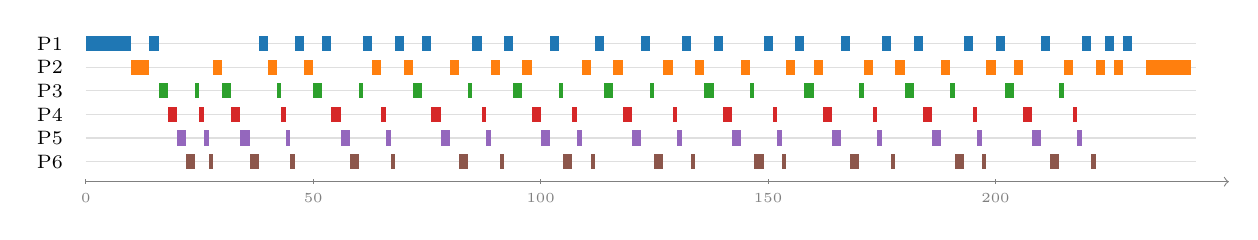
\begin{tikzpicture}[x=0.05777cm,y=0.30cm]
\node[anchor=east,font=\scriptsize] at (-2.9,5) {P1};
\draw[gray!25] (0,5) -- (244,5);
\node[anchor=east,font=\scriptsize] at (-2.9,4) {P2};
\draw[gray!25] (0,4) -- (244,4);
\node[anchor=east,font=\scriptsize] at (-2.9,3) {P3};
\draw[gray!25] (0,3) -- (244,3);
\node[anchor=east,font=\scriptsize] at (-2.9,2) {P4};
\draw[gray!25] (0,2) -- (244,2);
\node[anchor=east,font=\scriptsize] at (-2.9,1) {P5};
\draw[gray!25] (0,1) -- (244,1);
\node[anchor=east,font=\scriptsize] at (-2.9,0) {P6};
\draw[gray!25] (0,0) -- (244,0);
\fill[cP1] (0,4.68) rectangle (10,5.32);
\fill[cP2] (10,3.68) rectangle (14,4.32);
\fill[cP1] (14,4.68) rectangle (16,5.32);
\fill[cP3] (16,2.68) rectangle (18,3.32);
\fill[cP4] (18,1.68) rectangle (20,2.32);
\fill[cP5] (20,0.68) rectangle (22,1.32);
\fill[cP6] (22,-0.32) rectangle (24,0.32);
\fill[cP3] (24,2.68) rectangle (25,3.32);
\fill[cP4] (25,1.68) rectangle (26,2.32);
\fill[cP5] (26,0.68) rectangle (27,1.32);
\fill[cP6] (27,-0.32) rectangle (28,0.32);
\fill[cP2] (28,3.68) rectangle (30,4.32);
\fill[cP3] (30,2.68) rectangle (32,3.32);
\fill[cP4] (32,1.68) rectangle (34,2.32);
\fill[cP5] (34,0.68) rectangle (36,1.32);
\fill[cP6] (36,-0.32) rectangle (38,0.32);
\fill[cP1] (38,4.68) rectangle (40,5.32);
\fill[cP2] (40,3.68) rectangle (42,4.32);
\fill[cP3] (42,2.68) rectangle (43,3.32);
\fill[cP4] (43,1.68) rectangle (44,2.32);
\fill[cP5] (44,0.68) rectangle (45,1.32);
\fill[cP6] (45,-0.32) rectangle (46,0.32);
\fill[cP1] (46,4.68) rectangle (48,5.32);
\fill[cP2] (48,3.68) rectangle (50,4.32);
\fill[cP3] (50,2.68) rectangle (52,3.32);
\fill[cP1] (52,4.68) rectangle (54,5.32);
\fill[cP4] (54,1.68) rectangle (56,2.32);
\fill[cP5] (56,0.68) rectangle (58,1.32);
\fill[cP6] (58,-0.32) rectangle (60,0.32);
\fill[cP3] (60,2.68) rectangle (61,3.32);
\fill[cP1] (61,4.68) rectangle (63,5.32);
\fill[cP2] (63,3.68) rectangle (65,4.32);
\fill[cP4] (65,1.68) rectangle (66,2.32);
\fill[cP5] (66,0.68) rectangle (67,1.32);
\fill[cP6] (67,-0.32) rectangle (68,0.32);
\fill[cP1] (68,4.68) rectangle (70,5.32);
\fill[cP2] (70,3.68) rectangle (72,4.32);
\fill[cP3] (72,2.68) rectangle (74,3.32);
\fill[cP1] (74,4.68) rectangle (76,5.32);
\fill[cP4] (76,1.68) rectangle (78,2.32);
\fill[cP5] (78,0.68) rectangle (80,1.32);
\fill[cP2] (80,3.68) rectangle (82,4.32);
\fill[cP6] (82,-0.32) rectangle (84,0.32);
\fill[cP3] (84,2.68) rectangle (85,3.32);
\fill[cP1] (85,4.68) rectangle (87,5.32);
\fill[cP4] (87,1.68) rectangle (88,2.32);
\fill[cP5] (88,0.68) rectangle (89,1.32);
\fill[cP2] (89,3.68) rectangle (91,4.32);
\fill[cP6] (91,-0.32) rectangle (92,0.32);
\fill[cP1] (92,4.68) rectangle (94,5.32);
\fill[cP3] (94,2.68) rectangle (96,3.32);
\fill[cP2] (96,3.68) rectangle (98,4.32);
\fill[cP4] (98,1.68) rectangle (100,2.32);
\fill[cP5] (100,0.68) rectangle (102,1.32);
\fill[cP1] (102,4.68) rectangle (104,5.32);
\fill[cP3] (104,2.68) rectangle (105,3.32);
\fill[cP6] (105,-0.32) rectangle (107,0.32);
\fill[cP4] (107,1.68) rectangle (108,2.32);
\fill[cP5] (108,0.68) rectangle (109,1.32);
\fill[cP2] (109,3.68) rectangle (111,4.32);
\fill[cP6] (111,-0.32) rectangle (112,0.32);
\fill[cP1] (112,4.68) rectangle (114,5.32);
\fill[cP3] (114,2.68) rectangle (116,3.32);
\fill[cP2] (116,3.68) rectangle (118,4.32);
\fill[cP4] (118,1.68) rectangle (120,2.32);
\fill[cP5] (120,0.68) rectangle (122,1.32);
\fill[cP1] (122,4.68) rectangle (124,5.32);
\fill[cP3] (124,2.68) rectangle (125,3.32);
\fill[cP6] (125,-0.32) rectangle (127,0.32);
\fill[cP2] (127,3.68) rectangle (129,4.32);
\fill[cP4] (129,1.68) rectangle (130,2.32);
\fill[cP5] (130,0.68) rectangle (131,1.32);
\fill[cP1] (131,4.68) rectangle (133,5.32);
\fill[cP6] (133,-0.32) rectangle (134,0.32);
\fill[cP2] (134,3.68) rectangle (136,4.32);
\fill[cP3] (136,2.68) rectangle (138,3.32);
\fill[cP1] (138,4.68) rectangle (140,5.32);
\fill[cP4] (140,1.68) rectangle (142,2.32);
\fill[cP5] (142,0.68) rectangle (144,1.32);
\fill[cP2] (144,3.68) rectangle (146,4.32);
\fill[cP3] (146,2.68) rectangle (147,3.32);
\fill[cP6] (147,-0.32) rectangle (149,0.32);
\fill[cP1] (149,4.68) rectangle (151,5.32);
\fill[cP4] (151,1.68) rectangle (152,2.32);
\fill[cP5] (152,0.68) rectangle (153,1.32);
\fill[cP6] (153,-0.32) rectangle (154,0.32);
\fill[cP2] (154,3.68) rectangle (156,4.32);
\fill[cP1] (156,4.68) rectangle (158,5.32);
\fill[cP3] (158,2.68) rectangle (160,3.32);
\fill[cP2] (160,3.68) rectangle (162,4.32);
\fill[cP4] (162,1.68) rectangle (164,2.32);
\fill[cP5] (164,0.68) rectangle (166,1.32);
\fill[cP1] (166,4.68) rectangle (168,5.32);
\fill[cP6] (168,-0.32) rectangle (170,0.32);
\fill[cP3] (170,2.68) rectangle (171,3.32);
\fill[cP2] (171,3.68) rectangle (173,4.32);
\fill[cP4] (173,1.68) rectangle (174,2.32);
\fill[cP5] (174,0.68) rectangle (175,1.32);
\fill[cP1] (175,4.68) rectangle (177,5.32);
\fill[cP6] (177,-0.32) rectangle (178,0.32);
\fill[cP2] (178,3.68) rectangle (180,4.32);
\fill[cP3] (180,2.68) rectangle (182,3.32);
\fill[cP1] (182,4.68) rectangle (184,5.32);
\fill[cP4] (184,1.68) rectangle (186,2.32);
\fill[cP5] (186,0.68) rectangle (188,1.32);
\fill[cP2] (188,3.68) rectangle (190,4.32);
\fill[cP3] (190,2.68) rectangle (191,3.32);
\fill[cP6] (191,-0.32) rectangle (193,0.32);
\fill[cP1] (193,4.68) rectangle (195,5.32);
\fill[cP4] (195,1.68) rectangle (196,2.32);
\fill[cP5] (196,0.68) rectangle (197,1.32);
\fill[cP6] (197,-0.32) rectangle (198,0.32);
\fill[cP2] (198,3.68) rectangle (200,4.32);
\fill[cP1] (200,4.68) rectangle (202,5.32);
\fill[cP3] (202,2.68) rectangle (204,3.32);
\fill[cP2] (204,3.68) rectangle (206,4.32);
\fill[cP4] (206,1.68) rectangle (208,2.32);
\fill[cP5] (208,0.68) rectangle (210,1.32);
\fill[cP1] (210,4.68) rectangle (212,5.32);
\fill[cP6] (212,-0.32) rectangle (214,0.32);
\fill[cP3] (214,2.68) rectangle (215,3.32);
\fill[cP2] (215,3.68) rectangle (217,4.32);
\fill[cP4] (217,1.68) rectangle (218,2.32);
\fill[cP5] (218,0.68) rectangle (219,1.32);
\fill[cP1] (219,4.68) rectangle (221,5.32);
\fill[cP6] (221,-0.32) rectangle (222,0.32);
\fill[cP2] (222,3.68) rectangle (224,4.32);
\fill[cP1] (224,4.68) rectangle (226,5.32);
\fill[cP2] (226,3.68) rectangle (228,4.32);
\fill[cP1] (228,4.68) rectangle (230,5.32);
\fill[cP2] (233,3.68) rectangle (243,4.32);
\draw[->,gray] (0,-0.85) -- (251.3,-0.85);
\draw[gray] (0,-0.75)--(0,-0.95) node[below,font=\tiny]{0};
\draw[gray] (50,-0.75)--(50,-0.95) node[below,font=\tiny]{50};
\draw[gray] (100,-0.75)--(100,-0.95) node[below,font=\tiny]{100};
\draw[gray] (150,-0.75)--(150,-0.95) node[below,font=\tiny]{150};
\draw[gray] (200,-0.75)--(200,-0.95) node[below,font=\tiny]{200};
\end{tikzpicture}\par
\par\vspace{1.5mm}{\small\textbf{MLFQ-WB}\quad(makespan 243, idle 3)}\par\vspace{0.8mm}
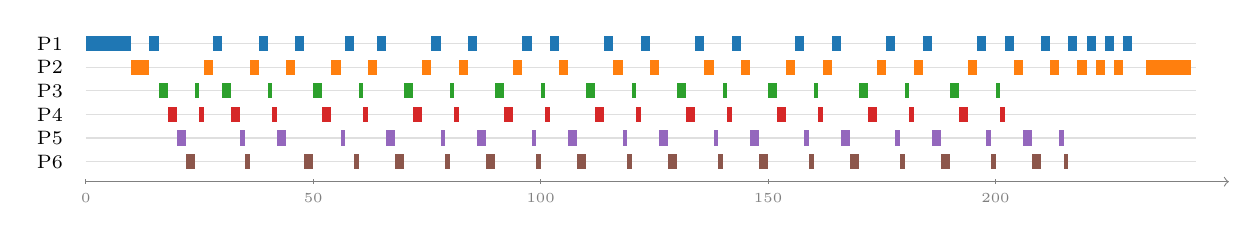
\begin{tikzpicture}[x=0.05777cm,y=0.30cm]
\node[anchor=east,font=\scriptsize] at (-2.9,5) {P1};
\draw[gray!25] (0,5) -- (244,5);
\node[anchor=east,font=\scriptsize] at (-2.9,4) {P2};
\draw[gray!25] (0,4) -- (244,4);
\node[anchor=east,font=\scriptsize] at (-2.9,3) {P3};
\draw[gray!25] (0,3) -- (244,3);
\node[anchor=east,font=\scriptsize] at (-2.9,2) {P4};
\draw[gray!25] (0,2) -- (244,2);
\node[anchor=east,font=\scriptsize] at (-2.9,1) {P5};
\draw[gray!25] (0,1) -- (244,1);
\node[anchor=east,font=\scriptsize] at (-2.9,0) {P6};
\draw[gray!25] (0,0) -- (244,0);
\fill[cP1] (0,4.68) rectangle (10,5.32);
\fill[cP2] (10,3.68) rectangle (14,4.32);
\fill[cP1] (14,4.68) rectangle (16,5.32);
\fill[cP3] (16,2.68) rectangle (18,3.32);
\fill[cP4] (18,1.68) rectangle (20,2.32);
\fill[cP5] (20,0.68) rectangle (22,1.32);
\fill[cP6] (22,-0.32) rectangle (24,0.32);
\fill[cP3] (24,2.68) rectangle (25,3.32);
\fill[cP4] (25,1.68) rectangle (26,2.32);
\fill[cP2] (26,3.68) rectangle (28,4.32);
\fill[cP1] (28,4.68) rectangle (30,5.32);
\fill[cP3] (30,2.68) rectangle (32,3.32);
\fill[cP4] (32,1.68) rectangle (34,2.32);
\fill[cP5] (34,0.68) rectangle (35,1.32);
\fill[cP6] (35,-0.32) rectangle (36,0.32);
\fill[cP2] (36,3.68) rectangle (38,4.32);
\fill[cP1] (38,4.68) rectangle (40,5.32);
\fill[cP3] (40,2.68) rectangle (41,3.32);
\fill[cP4] (41,1.68) rectangle (42,2.32);
\fill[cP5] (42,0.68) rectangle (44,1.32);
\fill[cP2] (44,3.68) rectangle (46,4.32);
\fill[cP1] (46,4.68) rectangle (48,5.32);
\fill[cP6] (48,-0.32) rectangle (50,0.32);
\fill[cP3] (50,2.68) rectangle (52,3.32);
\fill[cP4] (52,1.68) rectangle (54,2.32);
\fill[cP2] (54,3.68) rectangle (56,4.32);
\fill[cP5] (56,0.68) rectangle (57,1.32);
\fill[cP1] (57,4.68) rectangle (59,5.32);
\fill[cP6] (59,-0.32) rectangle (60,0.32);
\fill[cP3] (60,2.68) rectangle (61,3.32);
\fill[cP4] (61,1.68) rectangle (62,2.32);
\fill[cP2] (62,3.68) rectangle (64,4.32);
\fill[cP1] (64,4.68) rectangle (66,5.32);
\fill[cP5] (66,0.68) rectangle (68,1.32);
\fill[cP6] (68,-0.32) rectangle (70,0.32);
\fill[cP3] (70,2.68) rectangle (72,3.32);
\fill[cP4] (72,1.68) rectangle (74,2.32);
\fill[cP2] (74,3.68) rectangle (76,4.32);
\fill[cP1] (76,4.68) rectangle (78,5.32);
\fill[cP5] (78,0.68) rectangle (79,1.32);
\fill[cP6] (79,-0.32) rectangle (80,0.32);
\fill[cP3] (80,2.68) rectangle (81,3.32);
\fill[cP4] (81,1.68) rectangle (82,2.32);
\fill[cP2] (82,3.68) rectangle (84,4.32);
\fill[cP1] (84,4.68) rectangle (86,5.32);
\fill[cP5] (86,0.68) rectangle (88,1.32);
\fill[cP6] (88,-0.32) rectangle (90,0.32);
\fill[cP3] (90,2.68) rectangle (92,3.32);
\fill[cP4] (92,1.68) rectangle (94,2.32);
\fill[cP2] (94,3.68) rectangle (96,4.32);
\fill[cP1] (96,4.68) rectangle (98,5.32);
\fill[cP5] (98,0.68) rectangle (99,1.32);
\fill[cP6] (99,-0.32) rectangle (100,0.32);
\fill[cP3] (100,2.68) rectangle (101,3.32);
\fill[cP4] (101,1.68) rectangle (102,2.32);
\fill[cP1] (102,4.68) rectangle (104,5.32);
\fill[cP2] (104,3.68) rectangle (106,4.32);
\fill[cP5] (106,0.68) rectangle (108,1.32);
\fill[cP6] (108,-0.32) rectangle (110,0.32);
\fill[cP3] (110,2.68) rectangle (112,3.32);
\fill[cP4] (112,1.68) rectangle (114,2.32);
\fill[cP1] (114,4.68) rectangle (116,5.32);
\fill[cP2] (116,3.68) rectangle (118,4.32);
\fill[cP5] (118,0.68) rectangle (119,1.32);
\fill[cP6] (119,-0.32) rectangle (120,0.32);
\fill[cP3] (120,2.68) rectangle (121,3.32);
\fill[cP4] (121,1.68) rectangle (122,2.32);
\fill[cP1] (122,4.68) rectangle (124,5.32);
\fill[cP2] (124,3.68) rectangle (126,4.32);
\fill[cP5] (126,0.68) rectangle (128,1.32);
\fill[cP6] (128,-0.32) rectangle (130,0.32);
\fill[cP3] (130,2.68) rectangle (132,3.32);
\fill[cP4] (132,1.68) rectangle (134,2.32);
\fill[cP1] (134,4.68) rectangle (136,5.32);
\fill[cP2] (136,3.68) rectangle (138,4.32);
\fill[cP5] (138,0.68) rectangle (139,1.32);
\fill[cP6] (139,-0.32) rectangle (140,0.32);
\fill[cP3] (140,2.68) rectangle (141,3.32);
\fill[cP4] (141,1.68) rectangle (142,2.32);
\fill[cP1] (142,4.68) rectangle (144,5.32);
\fill[cP2] (144,3.68) rectangle (146,4.32);
\fill[cP5] (146,0.68) rectangle (148,1.32);
\fill[cP6] (148,-0.32) rectangle (150,0.32);
\fill[cP3] (150,2.68) rectangle (152,3.32);
\fill[cP4] (152,1.68) rectangle (154,2.32);
\fill[cP2] (154,3.68) rectangle (156,4.32);
\fill[cP1] (156,4.68) rectangle (158,5.32);
\fill[cP5] (158,0.68) rectangle (159,1.32);
\fill[cP6] (159,-0.32) rectangle (160,0.32);
\fill[cP3] (160,2.68) rectangle (161,3.32);
\fill[cP4] (161,1.68) rectangle (162,2.32);
\fill[cP2] (162,3.68) rectangle (164,4.32);
\fill[cP1] (164,4.68) rectangle (166,5.32);
\fill[cP5] (166,0.68) rectangle (168,1.32);
\fill[cP6] (168,-0.32) rectangle (170,0.32);
\fill[cP3] (170,2.68) rectangle (172,3.32);
\fill[cP4] (172,1.68) rectangle (174,2.32);
\fill[cP2] (174,3.68) rectangle (176,4.32);
\fill[cP1] (176,4.68) rectangle (178,5.32);
\fill[cP5] (178,0.68) rectangle (179,1.32);
\fill[cP6] (179,-0.32) rectangle (180,0.32);
\fill[cP3] (180,2.68) rectangle (181,3.32);
\fill[cP4] (181,1.68) rectangle (182,2.32);
\fill[cP2] (182,3.68) rectangle (184,4.32);
\fill[cP1] (184,4.68) rectangle (186,5.32);
\fill[cP5] (186,0.68) rectangle (188,1.32);
\fill[cP6] (188,-0.32) rectangle (190,0.32);
\fill[cP3] (190,2.68) rectangle (192,3.32);
\fill[cP4] (192,1.68) rectangle (194,2.32);
\fill[cP2] (194,3.68) rectangle (196,4.32);
\fill[cP1] (196,4.68) rectangle (198,5.32);
\fill[cP5] (198,0.68) rectangle (199,1.32);
\fill[cP6] (199,-0.32) rectangle (200,0.32);
\fill[cP3] (200,2.68) rectangle (201,3.32);
\fill[cP4] (201,1.68) rectangle (202,2.32);
\fill[cP1] (202,4.68) rectangle (204,5.32);
\fill[cP2] (204,3.68) rectangle (206,4.32);
\fill[cP5] (206,0.68) rectangle (208,1.32);
\fill[cP6] (208,-0.32) rectangle (210,0.32);
\fill[cP1] (210,4.68) rectangle (212,5.32);
\fill[cP2] (212,3.68) rectangle (214,4.32);
\fill[cP5] (214,0.68) rectangle (215,1.32);
\fill[cP6] (215,-0.32) rectangle (216,0.32);
\fill[cP1] (216,4.68) rectangle (218,5.32);
\fill[cP2] (218,3.68) rectangle (220,4.32);
\fill[cP1] (220,4.68) rectangle (222,5.32);
\fill[cP2] (222,3.68) rectangle (224,4.32);
\fill[cP1] (224,4.68) rectangle (226,5.32);
\fill[cP2] (226,3.68) rectangle (228,4.32);
\fill[cP1] (228,4.68) rectangle (230,5.32);
\fill[cP2] (233,3.68) rectangle (243,4.32);
\draw[->,gray] (0,-0.85) -- (251.3,-0.85);
\draw[gray] (0,-0.75)--(0,-0.95) node[below,font=\tiny]{0};
\draw[gray] (50,-0.75)--(50,-0.95) node[below,font=\tiny]{50};
\draw[gray] (100,-0.75)--(100,-0.95) node[below,font=\tiny]{100};
\draw[gray] (150,-0.75)--(150,-0.95) node[below,font=\tiny]{150};
\draw[gray] (200,-0.75)--(200,-0.95) node[below,font=\tiny]{200};
\end{tikzpicture}\par
\caption{Workload 5, single processor. The four short interactive processes P3--P6 all arrive at $t=15$. Under FIFO they queue behind P1 and P2; the preemptive policies interleave them immediately.}
\label{fig:gantt-single-5}
\end{figure}
\section{Additional Experiments}

\subsection{Effect of the Round Robin time quantum}

The assignment asks for Round Robin to be studied with different values of the time
quantum. The table reports the average turnaround time on the single processor for
$q \in \{1,2,4,8,16\}$ on all five workloads.

\begin{center}\small
\begin{tabular}{lrrrrr}
\toprule
\textbf{Workload} & $q=1$ & $q=2$ & $q=4$ & $q=8$ & $q=16$ \\
\midrule
Workload 1 & 459.33 & 458.67 & \textbf{458.00} & \textbf{458.00} & 463.33 \\
Workload 2 & 598.50 & \textbf{595.00} & 596.00 & 597.00 & 597.00 \\
Workload 3 & \textbf{14.50} & \textbf{14.50} & \textbf{14.50} & \textbf{14.50} & \textbf{14.50} \\
Workload 4 & 130.00 & 131.33 & 131.67 & \textbf{128.33} & 129.00 \\
Workload 5 & 203.83 & 215.67 & 207.17 & 205.67 & \textbf{196.33} \\
\bottomrule
\end{tabular}
\end{center}
\noindent The best quantum for each workload is shown in bold. Because the absolute
turnaround times differ by more than an order of magnitude between workloads, the graph
below normalises each workload against its own best quantum, so that all five curves can
be compared on a single set of axes.

\begin{figure}[htbp]\centering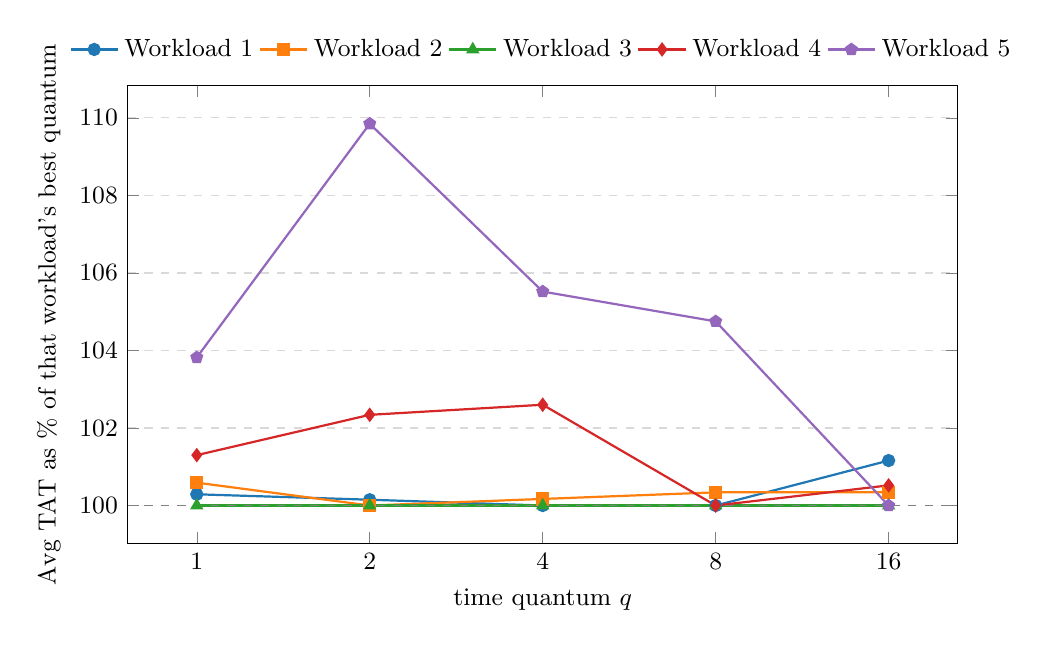
\begin{tikzpicture}
\begin{axis}[width=\textwidth, height=7.4cm, xlabel={time quantum $q$}, ylabel={Avg TAT as \% of that workload's best quantum},
  xtick={1,2,4,8,16}, xmode=log, log basis x=2, xticklabels={1,2,4,8,16},
  ymajorgrids, grid style={dashed,gray!30},
  legend style={at={(0.5,1.03)},anchor=south,legend columns=5,draw=none,font=\small},
  tick label style={font=\small}, label style={font=\small}]
\addplot[color=cP1,mark=*,thick,mark size=2pt] coordinates {(1,100.29) (2,100.15) (4,100.00) (8,100.00) (16,101.16)};
\addplot[color=cP2,mark=square*,thick,mark size=2pt] coordinates {(1,100.59) (2,100.00) (4,100.17) (8,100.34) (16,100.34)};
\addplot[color=cP3,mark=triangle*,thick,mark size=2pt] coordinates {(1,100.00) (2,100.00) (4,100.00) (8,100.00) (16,100.00)};
\addplot[color=cP4,mark=diamond*,thick,mark size=2pt] coordinates {(1,101.30) (2,102.34) (4,102.60) (8,100.00) (16,100.52)};
\addplot[color=cP5,mark=pentagon*,thick,mark size=2pt] coordinates {(1,103.82) (2,109.85) (4,105.52) (8,104.75) (16,100.00)};
\draw[dashed,gray] ({rel axis cs:0,0}|-{axis cs:1,100}) -- ({rel axis cs:1,0}|-{axis cs:1,100});
\legend{Workload 1, Workload 2, Workload 3, Workload 4, Workload 5}
\end{axis}\end{tikzpicture}
\caption{Average turnaround time versus Round Robin time quantum on a single processor, all five workloads on one axis. Each curve is normalised against the best quantum for that workload (100\,\% = best). Workload 3 is perfectly flat because its 1-unit CPU bursts never reach any quantum; the others respond non-monotonically, showing that the quantum interacts with the specific burst lengths of the workload.}
\end{figure}
\subsection{Effect of the MLFQ priority boost interval}

The assignment asks for a no-boost experiment to be compared against a boost every 20
time units. To place that comparison in context, the boost interval $B$ was swept over
$\{0,5,10,20,40,80\}$ on the single processor, where $B=0$ means boosting is disabled.

\begin{center}\small
\begin{tabular}{lrrrrrr}
\toprule
\textbf{Workload} & $B=0$ (off) & $B=5$ & $B=10$ & $B=20$ & $B=40$ & $B=80$ \\
\midrule
Workload 1 & 461.33 & \textbf{449.67} & 458.67 & 461.33 & 461.33 & 461.33 \\
Workload 2 & \textbf{595.00} & 597.50 & 597.00 & 597.00 & 597.00 & 596.00 \\
Workload 3 & \textbf{14.50} & \textbf{14.50} & \textbf{14.50} & \textbf{14.50} & \textbf{14.50} & \textbf{14.50} \\
Workload 4 & 135.33 & 124.67 & \textbf{124.33} & 131.67 & 136.67 & 135.33 \\
Workload 5 & 212.83 & 208.00 & 207.17 & 206.17 & \textbf{198.17} & 202.17 \\
\bottomrule
\end{tabular}
\end{center}
\begin{figure}[htbp]\centering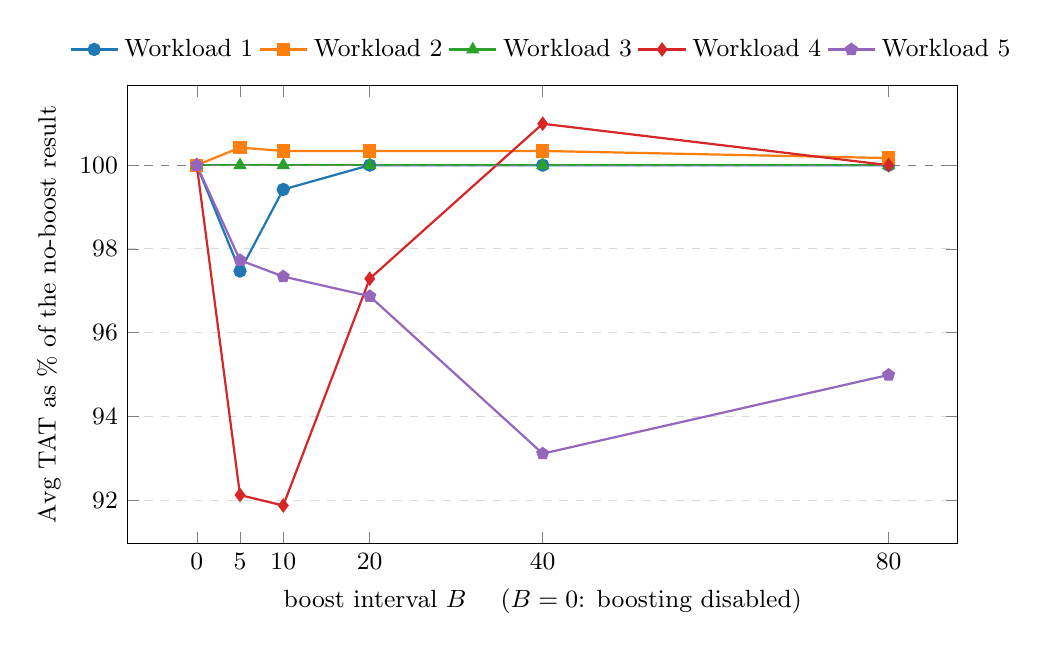
\begin{tikzpicture}
\begin{axis}[width=\textwidth, height=7.4cm, xlabel={boost interval $B$ \quad($B=0$: boosting disabled)}, ylabel={Avg TAT as \% of the no-boost result},
  xtick={0,5,10,20,40,80}, 
  ymajorgrids, grid style={dashed,gray!30},
  legend style={at={(0.5,1.03)},anchor=south,legend columns=5,draw=none,font=\small},
  tick label style={font=\small}, label style={font=\small}]
\addplot[color=cP1,mark=*,thick,mark size=2pt] coordinates {(0,100.00) (5,97.47) (10,99.42) (20,100.00) (40,100.00) (80,100.00)};
\addplot[color=cP2,mark=square*,thick,mark size=2pt] coordinates {(0,100.00) (5,100.42) (10,100.34) (20,100.34) (40,100.34) (80,100.17)};
\addplot[color=cP3,mark=triangle*,thick,mark size=2pt] coordinates {(0,100.00) (5,100.00) (10,100.00) (20,100.00) (40,100.00) (80,100.00)};
\addplot[color=cP4,mark=diamond*,thick,mark size=2pt] coordinates {(0,100.00) (5,92.12) (10,91.87) (20,97.29) (40,100.99) (80,100.00)};
\addplot[color=cP5,mark=pentagon*,thick,mark size=2pt] coordinates {(0,100.00) (5,97.73) (10,97.34) (20,96.87) (40,93.11) (80,94.99)};
\draw[dashed,gray] ({rel axis cs:0,0}|-{axis cs:0,100}) -- ({rel axis cs:1,0}|-{axis cs:0,100});
\legend{Workload 1, Workload 2, Workload 3, Workload 4, Workload 5}
\end{axis}\end{tikzpicture}
\caption{Average turnaround time versus MLFQ priority boost interval on a single processor, all five workloads on one axis. Each curve is normalised against that workload's own no-boost result ($B=0$), so the dashed 100\,\% line is ``no boost at all'' and any point \emph{below} it means boosting improved the average turnaround time. Workload 3 is flat because no demotion ever occurs, so a boost has nothing to undo.}
\end{figure}
\newpage
\section{Findings and Analysis}
\subsection{Finding 1: FIFO has the lowest \emph{average} turnaround time}

On a single processor FIFO produced the lowest average turnaround time on four workloads and
tied with every other policy on workload 3:

\begin{center}\small
\begin{tabular}{lrrrr}
\toprule
\textbf{Workload} & \textbf{FIFO} & \textbf{RR} & \textbf{MLFQ-NB} & \textbf{MLFQ-WB}\\
\midrule
Workload 1 & \textbf{363.33} & 458.67 & 461.33 & 461.33 \\
Workload 2 & \textbf{525.00} & 595.00 & 595.00 & 597.00 \\
Workload 3 & \textbf{14.50} & 14.50 & 14.50 & 14.50 \\
Workload 4 & \textbf{123.00} & 131.33 & 135.33 & 131.67 \\
Workload 5 & \textbf{189.00} & 215.67 & 212.83 & 206.17 \\
\bottomrule\end{tabular}\end{center}

This is not an accident and it is not a defect of the preemptive policies. Average
turnaround time rewards letting \emph{some} processes finish as early as possible. FIFO runs
one process to the end of its burst before starting another, so early processes complete
early. Round Robin and MLFQ interleave every runnable process, so they all make progress
together and consequently tend to finish at similar, later times.

Workload 1 shows this in its purest form. It contains three pure CPU-bound processes (200,
100 and 300 units) with no I/O at all, so the total work is 600 units and \emph{every}
policy has a makespan of exactly 600 --- the CPU is never idle and nothing can change the
finishing time of the last process. The policies differ only in \emph{when the first two}
processes finish:

\begin{center}\small
\begin{tabular}{lrrr}
\toprule
\textbf{Policy} & \textbf{P1 finishes} & \textbf{P2 finishes} & \textbf{P3 finishes}\\
\midrule
FIFO & 200 & 300 & 600 \\
RR & 492 & 294 & 600 \\
MLFQ-NB & 496 & 298 & 600 \\
MLFQ-WB & 496 & 298 & 600 \\
\bottomrule\end{tabular}\end{center}

Under FIFO, P1 finishes at time 200 and P2 at 300. Under Round Robin, P1 is dragged out to 492
--- 292 time units later --- while P2 finishes at 294, only 6 time units \emph{earlier}. P3
finishes at 600 in both cases. Time-slicing therefore made one process much slower in
exchange for a tiny gain for another, which is exactly why the average rises from 363.33 to
458.67.

\subsection{Finding 2: FIFO loses badly on \emph{worst-case} turnaround time}

Average turnaround time alone is a misleading summary. On workload 4 the ranking reverses
when the maximum is considered:

\begin{center}\small
\begin{tabular}{lrrrr}
\toprule
\textbf{Workload 4} & \textbf{FIFO} & \textbf{RR} & \textbf{MLFQ-NB} & \textbf{MLFQ-WB}\\
\midrule
Average TAT & 123.00 & 131.33 & 135.33 & 131.67 \\
Maximum TAT & 163 & 142 & 144 & 147 \\
Minimum TAT & 73 & 126 & 127 & 112 \\
\bottomrule\end{tabular}\end{center}

FIFO's worst-case turnaround is 163, versus 142 for Round Robin --- and its spread between the
best- and worst-served process is 73 to 163, a range of 90 time units. Round Robin's spread is
only 126 to 142, a range of 16. This is the \textbf{convoy effect}: workload 4's P1 is a
30-unit CPU-bound process, and under FIFO the 3-unit interactive process P3 must wait behind
it every single time. FIFO achieves a good average by being extremely unfair.

If the goal is an interactive system, the maximum and the spread matter far more than the
mean, and on that criterion every preemptive policy beats FIFO here.

\subsection{Finding 3: preemption dramatically improves CPU utilisation}

The most practically important result concerns how well each policy overlaps I/O with
computation:

\begin{center}\small
\begin{tabular}{lrrrr}
\toprule
\textbf{Workload 4} & \textbf{FIFO} & \textbf{RR} & \textbf{MLFQ-NB} & \textbf{MLFQ-WB}\\
\midrule
Run time (CPU busy) & 150 & 150 & 150 & 150 \\
Makespan & 178 & 152 & 154 & 157 \\
Idle time & 28 & 2 & 4 & 7 \\
Utilisation & 84.3\% & 98.7\% & 97.4\% & 95.5\% \\
\bottomrule\end{tabular}\end{center}

All four policies must execute the same 150 units of CPU work, so run time is identical.
What differs is how much time is \emph{wasted}. FIFO idles the CPU for 28 time units
(84.3\,\% utilisation) because it lets each process run its full burst, which delays the
moment the other processes issue their I/O requests; eventually all three are blocked
simultaneously and the CPU has nothing to do. Round Robin idles for only 2 units
(98.7\,\%), because slicing forces every process to reach its I/O request early, so I/O
requests are spread out and overlap with computation.

The consequence is that Round Robin finishes the entire workload at time 152 instead of
FIFO's 178 --- \textbf{26 time units, or 15\,\%, sooner}. On a real machine this is the
difference between a saturated CPU and one sitting idle waiting for disks.

\subsection{Finding 4: the priority boost trades worst case for average}

Comparing MLFQ with and without the boost:

\begin{center}\small
\begin{tabular}{lrrrr}
\toprule
& \multicolumn{2}{c}{\textbf{Workload 4}} & \multicolumn{2}{c}{\textbf{Workload 5}}\\
\cmidrule(lr){2-3}\cmidrule(lr){4-5}
& \textbf{No boost} & \textbf{Boost 20} & \textbf{No boost} & \textbf{Boost 20}\\
\midrule
Average TAT & 135.33 & 131.67 & 212.83 & 206.17 \\
Maximum TAT & 144 & 147 & 233 & 233 \\
Minimum TAT & 127 & 112 & 200 & 186 \\
\bottomrule\end{tabular}\end{center}

On both mixed workloads the boost \emph{improves} the average turnaround time
(135.33 $\rightarrow$ 131.67 on workload 4; 212.83 $\rightarrow$ 206.17 on workload 5). On workload 4
it simultaneously makes the \emph{maximum} slightly worse (144 $\rightarrow$ 147).

The mechanism is visible in the minimum turnaround column: on workload 4 the boost improves
the best-served process from 127 to 112. Boosting periodically lifts processes that have sunk
to $Q_2$ back into $Q_0$, letting them make a burst of progress they would otherwise have
made much later. That helps those processes (and the average), while the short processes
occasionally have to queue behind a freshly promoted long process, which costs them a little
in the worst case.

This is precisely the trade-off the boost is designed to make: it sacrifices the
scheduler's accumulated knowledge of which processes are CPU-bound, in exchange for a hard
guarantee that no process waits more than $B$ time units at low priority.

\subsection{Finding 5: neither parameter is monotonic}

Neither the Round Robin quantum nor the boost interval has a simple ``bigger is better''
relationship with turnaround time. On workload 5 the average turnaround time under Round
Robin is $203.83$, $215.67$, $207.17$, $205.67$ and $196.33$ for $q=1,2,4,8,16$ respectively --- it gets
worse from $q=1$ to $q=2$, then improves steadily. On workload 4 the best boost interval was
$B=10$ rather than the assignment's $B=20$, and $B=40$ (136.67) was worse than no boost at all
(135.33).

The reason is that these parameters interact with the specific burst lengths of the
workload. A quantum that happens to align with a common burst length causes many processes
to finish exactly at a quantum boundary, changing the queue order for everything that
follows. There is therefore no universally optimal quantum; it must be tuned to the expected
workload.

\subsection{Finding 6: when all four algorithms coincide}

Workload 3 produced \emph{identical} results for all four policies: average 14.50, maximum
16, minimum 13, makespan 16. Every CPU burst in workload 3 is exactly 1 time unit long, and
both Round Robin and MLFQ use a quantum of 2. A burst therefore always completes before the
quantum can expire, so preemption never fires and no MLFQ demotion ever occurs. With no
demotions, every process stays in $Q_0$ forever and the boost has nothing to do. All three
policies degenerate to plain FIFO.

This is a useful sanity check on the implementation, and it illustrates a real principle: a
scheduling policy can only differentiate itself when the quantum is small relative to the
burst lengths.

\subsection{Finding 7: the hidden cost of preemption}

Counting the number of contiguous CPU segments gives a proxy for context-switch overhead:

\begin{center}\small
\begin{tabular}{lrrrr}
\toprule
\textbf{Workload} & \textbf{FIFO} & \textbf{RR} & \textbf{MLFQ-NB} & \textbf{MLFQ-WB}\\
\midrule
Workload 1 & 3 & 247 & 248 & 248 \\
Workload 2 & 12 & 300 & 300 & 300 \\
Workload 3 & 12 & 12 & 12 & 12 \\
Workload 4 & 18 & 68 & 67 & 62 \\
Workload 5 & 48 & 131 & 131 & 131 \\
\bottomrule\end{tabular}\end{center}

On workload 1 FIFO needs 3 dispatches while Round Robin needs 247 --- over 82 times more.
The simulator models context switches as free, so this cost does not appear in any of the
turnaround numbers. On real hardware each switch costs pipeline flushes, TLB and cache
pollution, and scheduler bookkeeping. A complete evaluation would have to weigh Round Robin's
better responsiveness against this overhead, and it is the main practical reason why real
systems do not use a quantum of 1.

\section{Summary of Part I}

\begin{center}\small
\begin{tabular}{l>{\raggedright\arraybackslash}p{4.1cm}>{\raggedright\arraybackslash}p{4.1cm}>{\raggedright\arraybackslash}p{3.2cm}}
\toprule
\textbf{Policy} & \textbf{Strengths} & \textbf{Weaknesses} & \textbf{Best suited to}\\
\midrule
FIFO & Lowest average turnaround on every workload (tied on W3); minimal context-switch
overhead; trivial to implement; no starvation & Severe convoy effect; worst maximum turnaround
(163 on W4); poor CPU utilisation (84.3\,\% on W4); no responsiveness & Batch systems where
throughput matters and latency does not \\ \addlinespace
Round Robin & Bounded waiting; excellent fairness (W4 spread only 16 units); best CPU
utilisation (98.7\,\% on W4); shortest makespan on W4 & Worse average turnaround than FIFO
on every workload except W3; very high switch count; performance sensitive to $q$; cannot distinguish process
types & Time-sharing systems with similar processes \\ \addlinespace
MLFQ (no boost) & Infers process behaviour with no prior knowledge; favours interactive
jobs; good utilisation (97.4\,\% on W4) & CPU-bound jobs can starve in $Q_2$; can be gamed by
yielding before quantum expiry & General-purpose systems with mixed workloads \\ \addlinespace
MLFQ (boost 20) & Removes starvation entirely; improved average over no-boost on both
mixed workloads; adapts to changing behaviour & Discards learned priority information;
slightly worse maximum on W4; $B$ needs tuning & Interactive general-purpose operating
systems \\
\bottomrule
\end{tabular}
\end{center}

On a single processor, no algorithm is best on every metric. FIFO wins on average
turnaround time; the preemptive policies win on worst-case turnaround, fairness and CPU
utilisation. MLFQ recovers most of Round Robin's fairness while automatically identifying
interactive processes, and the boost removes its starvation weakness at a small cost in the
worst case.
\newpage\part{Dual Processor}
\section{Overview of Part II}

Part II repeats every experiment of Part I on the dual-processor simulator described in
Section~\ref{sec:dualdesign}: the same five workloads, the same four policies, the same quantum of 2 and
boost interval of 20, and the same parameter sweeps. Only the number of processors has
changed. The structure of this part mirrors Part I exactly; a direct side-by-side
comparison of the two follows in Part III.

\section{Detailed Turnaround Time Calculations}

For every workload and every algorithm the tables below list, for each process, its
arrival time $A_i$, its finish time $F_i$ (the time unit at which its last CPU burst
completes) and its turnaround time $\mathrm{TAT}_i = F_i - A_i$, all measured on the
\textbf{dual processor}. The three summary rows give the average, maximum and minimum turnaround
time over all processes of that workload. \textbf{MLFQ-NB} denotes MLFQ with the boost
disabled and \textbf{MLFQ-WB} denotes MLFQ with a priority boost every 20 time units.
Round Robin uses a time quantum of 2, matching the MLFQ quantum so that the comparison is
fair.

A second table under each workload gives the processor-level figures: the busy time of
each CPU, the idle time summed over both CPUs, the utilisation of the pair of CPUs, and
the number of CPU bursts that \emph{migrated}, i.e.\ were started on one processor and
finished on the other.

\subsection{Workload 1}
\begin{center}\footnotesize\setlength{\tabcolsep}{4pt}
\begin{tabular}{cccccccccccccc}\toprule
& & \multicolumn{3}{c}{\textbf{FIFO}} & \multicolumn{3}{c}{\textbf{RR ($q=2$)}} & \multicolumn{3}{c}{\textbf{MLFQ-NB}} & \multicolumn{3}{c}{\textbf{MLFQ-WB}} \\
\cmidrule(lr){3-5}\cmidrule(lr){6-8}\cmidrule(lr){9-11}\cmidrule(lr){12-14}
Proc & $A_i$ & $F_i$ & $F_i-A_i$ & TAT & $F_i$ & $F_i-A_i$ & TAT & $F_i$ & $F_i-A_i$ & TAT & $F_i$ & $F_i-A_i$ & TAT \\\midrule
P1 & 0 & 200 & $200-0$ & 200 & 244 & $244-0$ & 244 & 246 & $246-0$ & 246 & 246 & $246-0$ & 246 \\
P2 & 0 & 100 & $100-0$ & 100 & 144 & $144-0$ & 144 & 146 & $146-0$ & 146 & 146 & $146-0$ & 146 \\
P3 & 10 & 400 & $400-10$ & 390 & 356 & $356-10$ & 346 & 354 & $354-10$ & 344 & 354 & $354-10$ & 344 \\
\midrule
\textbf{Average} & & \multicolumn{3}{c}{230.00} & \multicolumn{3}{c}{244.67} & \multicolumn{3}{c}{245.33} & \multicolumn{3}{c}{245.33} \\
\textbf{Maximum} & & \multicolumn{3}{c}{390} & \multicolumn{3}{c}{346} & \multicolumn{3}{c}{344} & \multicolumn{3}{c}{344} \\
\textbf{Minimum} & & \multicolumn{3}{c}{100} & \multicolumn{3}{c}{144} & \multicolumn{3}{c}{146} & \multicolumn{3}{c}{146} \\
\bottomrule\end{tabular}\end{center}
\begin{center}\footnotesize\begin{tabular}{lcccc}\toprule
& \textbf{FIFO} & \textbf{RR} & \textbf{MLFQ-NB} & \textbf{MLFQ-WB}\\\midrule
Run time CPU0 & 200 & 356 & 354 & 354 \\
Run time CPU1 & 400 & 244 & 246 & 246 \\
Run time, both CPUs & 600 & 600 & 600 & 600 \\
Total simulation time & 400 & 356 & 354 & 354 \\
Idle time, both CPUs & 200 & 112 & 108 & 108 \\
Utilisation of both CPUs & 75.0\% & 84.3\% & 84.7\% & 84.7\% \\
CPU segments (dispatches) & 3 & 136 & 140 & 140 \\
Bursts migrated between CPUs & 0 of 3 & 3 of 3 & 3 of 3 & 3 of 3 \\
\bottomrule\end{tabular}\end{center}

\subsection{Workload 2}
\begin{center}\footnotesize\setlength{\tabcolsep}{4pt}
\begin{tabular}{cccccccccccccc}\toprule
& & \multicolumn{3}{c}{\textbf{FIFO}} & \multicolumn{3}{c}{\textbf{RR ($q=2$)}} & \multicolumn{3}{c}{\textbf{MLFQ-NB}} & \multicolumn{3}{c}{\textbf{MLFQ-WB}} \\
\cmidrule(lr){3-5}\cmidrule(lr){6-8}\cmidrule(lr){9-11}\cmidrule(lr){12-14}
Proc & $A_i$ & $F_i$ & $F_i-A_i$ & TAT & $F_i$ & $F_i-A_i$ & TAT & $F_i$ & $F_i-A_i$ & TAT & $F_i$ & $F_i-A_i$ & TAT \\\midrule
P1 & 0 & 250 & $250-0$ & 250 & 304 & $304-0$ & 304 & 304 & $304-0$ & 304 & 304 & $304-0$ & 304 \\
P2 & 0 & 250 & $250-0$ & 250 & 304 & $304-0$ & 304 & 304 & $304-0$ & 304 & 304 & $304-0$ & 304 \\
P3 & 0 & 300 & $300-0$ & 300 & 306 & $306-0$ & 306 & 306 & $306-0$ & 306 & 306 & $306-0$ & 306 \\
P4 & 0 & 300 & $300-0$ & 300 & 306 & $306-0$ & 306 & 306 & $306-0$ & 306 & 306 & $306-0$ & 306 \\
\midrule
\textbf{Average} & & \multicolumn{3}{c}{275.00} & \multicolumn{3}{c}{305.00} & \multicolumn{3}{c}{305.00} & \multicolumn{3}{c}{305.00} \\
\textbf{Maximum} & & \multicolumn{3}{c}{300} & \multicolumn{3}{c}{306} & \multicolumn{3}{c}{306} & \multicolumn{3}{c}{306} \\
\textbf{Minimum} & & \multicolumn{3}{c}{250} & \multicolumn{3}{c}{304} & \multicolumn{3}{c}{304} & \multicolumn{3}{c}{304} \\
\bottomrule\end{tabular}\end{center}
\begin{center}\footnotesize\begin{tabular}{lcccc}\toprule
& \textbf{FIFO} & \textbf{RR} & \textbf{MLFQ-NB} & \textbf{MLFQ-WB}\\\midrule
Run time CPU0 & 300 & 300 & 300 & 300 \\
Run time CPU1 & 300 & 300 & 300 & 300 \\
Run time, both CPUs & 600 & 600 & 600 & 600 \\
Total simulation time & 300 & 306 & 306 & 306 \\
Idle time, both CPUs & 0 & 12 & 12 & 12 \\
Utilisation of both CPUs & 100.0\% & 98.0\% & 98.0\% & 98.0\% \\
CPU segments (dispatches) & 12 & 300 & 300 & 300 \\
Bursts migrated between CPUs & 0 of 12 & 0 of 12 & 0 of 12 & 0 of 12 \\
\bottomrule\end{tabular}\end{center}

\subsection{Workload 3}
\begin{center}\footnotesize\setlength{\tabcolsep}{4pt}
\begin{tabular}{cccccccccccccc}\toprule
& & \multicolumn{3}{c}{\textbf{FIFO}} & \multicolumn{3}{c}{\textbf{RR ($q=2$)}} & \multicolumn{3}{c}{\textbf{MLFQ-NB}} & \multicolumn{3}{c}{\textbf{MLFQ-WB}} \\
\cmidrule(lr){3-5}\cmidrule(lr){6-8}\cmidrule(lr){9-11}\cmidrule(lr){12-14}
Proc & $A_i$ & $F_i$ & $F_i-A_i$ & TAT & $F_i$ & $F_i-A_i$ & TAT & $F_i$ & $F_i-A_i$ & TAT & $F_i$ & $F_i-A_i$ & TAT \\\midrule
P1 & 0 & 13 & $13-0$ & 13 & 13 & $13-0$ & 13 & 13 & $13-0$ & 13 & 13 & $13-0$ & 13 \\
P2 & 0 & 13 & $13-0$ & 13 & 13 & $13-0$ & 13 & 13 & $13-0$ & 13 & 13 & $13-0$ & 13 \\
P3 & 0 & 14 & $14-0$ & 14 & 14 & $14-0$ & 14 & 14 & $14-0$ & 14 & 14 & $14-0$ & 14 \\
P4 & 0 & 14 & $14-0$ & 14 & 14 & $14-0$ & 14 & 14 & $14-0$ & 14 & 14 & $14-0$ & 14 \\
\midrule
\textbf{Average} & & \multicolumn{3}{c}{13.50} & \multicolumn{3}{c}{13.50} & \multicolumn{3}{c}{13.50} & \multicolumn{3}{c}{13.50} \\
\textbf{Maximum} & & \multicolumn{3}{c}{14} & \multicolumn{3}{c}{14} & \multicolumn{3}{c}{14} & \multicolumn{3}{c}{14} \\
\textbf{Minimum} & & \multicolumn{3}{c}{13} & \multicolumn{3}{c}{13} & \multicolumn{3}{c}{13} & \multicolumn{3}{c}{13} \\
\bottomrule\end{tabular}\end{center}
\begin{center}\footnotesize\begin{tabular}{lcccc}\toprule
& \textbf{FIFO} & \textbf{RR} & \textbf{MLFQ-NB} & \textbf{MLFQ-WB}\\\midrule
Run time CPU0 & 6 & 6 & 6 & 6 \\
Run time CPU1 & 6 & 6 & 6 & 6 \\
Run time, both CPUs & 12 & 12 & 12 & 12 \\
Total simulation time & 14 & 14 & 14 & 14 \\
Idle time, both CPUs & 16 & 16 & 16 & 16 \\
Utilisation of both CPUs & 42.9\% & 42.9\% & 42.9\% & 42.9\% \\
CPU segments (dispatches) & 12 & 12 & 12 & 12 \\
Bursts migrated between CPUs & 0 of 12 & 0 of 12 & 0 of 12 & 0 of 12 \\
\bottomrule\end{tabular}\end{center}

\subsection{Workload 4}
\begin{center}\footnotesize\setlength{\tabcolsep}{4pt}
\begin{tabular}{cccccccccccccc}\toprule
& & \multicolumn{3}{c}{\textbf{FIFO}} & \multicolumn{3}{c}{\textbf{RR ($q=2$)}} & \multicolumn{3}{c}{\textbf{MLFQ-NB}} & \multicolumn{3}{c}{\textbf{MLFQ-WB}} \\
\cmidrule(lr){3-5}\cmidrule(lr){6-8}\cmidrule(lr){9-11}\cmidrule(lr){12-14}
Proc & $A_i$ & $F_i$ & $F_i-A_i$ & TAT & $F_i$ & $F_i-A_i$ & TAT & $F_i$ & $F_i-A_i$ & TAT & $F_i$ & $F_i-A_i$ & TAT \\\midrule
P1 & 0 & 65 & $65-0$ & 65 & 69 & $69-0$ & 69 & 72 & $72-0$ & 72 & 73 & $73-0$ & 73 \\
P2 & 10 & 96 & $96-10$ & 86 & 101 & $101-10$ & 91 & 101 & $101-10$ & 91 & 100 & $100-10$ & 90 \\
P3 & 15 & 108 & $108-15$ & 93 & 94 & $94-15$ & 79 & 94 & $94-15$ & 79 & 93 & $93-15$ & 78 \\
\midrule
\textbf{Average} & & \multicolumn{3}{c}{81.33} & \multicolumn{3}{c}{79.67} & \multicolumn{3}{c}{80.67} & \multicolumn{3}{c}{80.33} \\
\textbf{Maximum} & & \multicolumn{3}{c}{93} & \multicolumn{3}{c}{91} & \multicolumn{3}{c}{91} & \multicolumn{3}{c}{90} \\
\textbf{Minimum} & & \multicolumn{3}{c}{65} & \multicolumn{3}{c}{69} & \multicolumn{3}{c}{72} & \multicolumn{3}{c}{73} \\
\bottomrule\end{tabular}\end{center}
\begin{center}\footnotesize\begin{tabular}{lcccc}\toprule
& \textbf{FIFO} & \textbf{RR} & \textbf{MLFQ-NB} & \textbf{MLFQ-WB}\\\midrule
Run time CPU0 & 95 & 90 & 90 & 91 \\
Run time CPU1 & 55 & 60 & 60 & 59 \\
Run time, both CPUs & 150 & 150 & 150 & 150 \\
Total simulation time & 108 & 101 & 101 & 100 \\
Idle time, both CPUs & 66 & 52 & 52 & 50 \\
Utilisation of both CPUs & 69.4\% & 74.3\% & 74.3\% & 75.0\% \\
CPU segments (dispatches) & 18 & 40 & 44 & 45 \\
Bursts migrated between CPUs & 0 of 18 & 11 of 18 & 12 of 18 & 11 of 18 \\
\bottomrule\end{tabular}\end{center}

\subsection{Workload 5}
\begin{center}\footnotesize\setlength{\tabcolsep}{4pt}
\begin{tabular}{cccccccccccccc}\toprule
& & \multicolumn{3}{c}{\textbf{FIFO}} & \multicolumn{3}{c}{\textbf{RR ($q=2$)}} & \multicolumn{3}{c}{\textbf{MLFQ-NB}} & \multicolumn{3}{c}{\textbf{MLFQ-WB}} \\
\cmidrule(lr){3-5}\cmidrule(lr){6-8}\cmidrule(lr){9-11}\cmidrule(lr){12-14}
Proc & $A_i$ & $F_i$ & $F_i-A_i$ & TAT & $F_i$ & $F_i-A_i$ & TAT & $F_i$ & $F_i-A_i$ & TAT & $F_i$ & $F_i-A_i$ & TAT \\\midrule
P1 & 0 & 70 & $70-0$ & 70 & 103 & $103-0$ & 103 & 106 & $106-0$ & 106 & 112 & $112-0$ & 112 \\
P2 & 10 & 111 & $111-10$ & 101 & 130 & $130-10$ & 120 & 133 & $133-10$ & 123 & 135 & $135-10$ & 125 \\
P3 & 15 & 125 & $125-15$ & 110 & 117 & $117-15$ & 102 & 115 & $115-15$ & 100 & 120 & $120-15$ & 105 \\
P4 & 15 & 128 & $128-15$ & 113 & 119 & $119-15$ & 104 & 118 & $118-15$ & 103 & 121 & $121-15$ & 106 \\
P5 & 15 & 130 & $130-15$ & 115 & 121 & $121-15$ & 106 & 121 & $121-15$ & 106 & 121 & $121-15$ & 106 \\
P6 & 15 & 131 & $131-15$ & 116 & 124 & $124-15$ & 109 & 122 & $122-15$ & 107 & 122 & $122-15$ & 107 \\
\midrule
\textbf{Average} & & \multicolumn{3}{c}{104.17} & \multicolumn{3}{c}{107.33} & \multicolumn{3}{c}{107.50} & \multicolumn{3}{c}{110.17} \\
\textbf{Maximum} & & \multicolumn{3}{c}{116} & \multicolumn{3}{c}{120} & \multicolumn{3}{c}{123} & \multicolumn{3}{c}{125} \\
\textbf{Minimum} & & \multicolumn{3}{c}{70} & \multicolumn{3}{c}{102} & \multicolumn{3}{c}{100} & \multicolumn{3}{c}{105} \\
\bottomrule\end{tabular}\end{center}
\begin{center}\footnotesize\begin{tabular}{lcccc}\toprule
& \textbf{FIFO} & \textbf{RR} & \textbf{MLFQ-NB} & \textbf{MLFQ-WB}\\\midrule
Run time CPU0 & 129 & 130 & 132 & 131 \\
Run time CPU1 & 111 & 110 & 108 & 109 \\
Run time, both CPUs & 240 & 240 & 240 & 240 \\
Total simulation time & 131 & 130 & 133 & 135 \\
Idle time, both CPUs & 22 & 20 & 26 & 30 \\
Utilisation of both CPUs & 91.6\% & 92.3\% & 90.2\% & 88.9\% \\
CPU segments (dispatches) & 48 & 123 & 120 & 113 \\
Bursts migrated between CPUs & 0 of 48 & 27 of 48 & 17 of 48 & 11 of 48 \\
\bottomrule\end{tabular}\end{center}

\newpage
\section{Consolidated Summary}

\begin{center}\small
\begin{tabular}{llrrrrrr}
\toprule
\textbf{Workload} & \textbf{Algorithm} & \textbf{Avg TAT} & \textbf{Max TAT} &
\textbf{Min TAT} & \textbf{Run time} & \textbf{Makespan} & \textbf{Util.} \\
\midrule
W1 & FIFO & 230.00 & 390 & 100 & 600 & 400 & 75.0\% \\
 & RR & 244.67 & 346 & 144 & 600 & 356 & 84.3\% \\
 & MLFQ-NB & 245.33 & 344 & 146 & 600 & 354 & 84.7\% \\
 & MLFQ-WB & 245.33 & 344 & 146 & 600 & 354 & 84.7\% \\
\midrule
W2 & FIFO & 275.00 & 300 & 250 & 600 & 300 & 100.0\% \\
 & RR & 305.00 & 306 & 304 & 600 & 306 & 98.0\% \\
 & MLFQ-NB & 305.00 & 306 & 304 & 600 & 306 & 98.0\% \\
 & MLFQ-WB & 305.00 & 306 & 304 & 600 & 306 & 98.0\% \\
\midrule
W3 & FIFO & 13.50 & 14 & 13 & 12 & 14 & 42.9\% \\
 & RR & 13.50 & 14 & 13 & 12 & 14 & 42.9\% \\
 & MLFQ-NB & 13.50 & 14 & 13 & 12 & 14 & 42.9\% \\
 & MLFQ-WB & 13.50 & 14 & 13 & 12 & 14 & 42.9\% \\
\midrule
W4 & FIFO & 81.33 & 93 & 65 & 150 & 108 & 69.4\% \\
 & RR & 79.67 & 91 & 69 & 150 & 101 & 74.3\% \\
 & MLFQ-NB & 80.67 & 91 & 72 & 150 & 101 & 74.3\% \\
 & MLFQ-WB & 80.33 & 90 & 73 & 150 & 100 & 75.0\% \\
\midrule
W5 & FIFO & 104.17 & 116 & 70 & 240 & 131 & 91.6\% \\
 & RR & 107.33 & 120 & 102 & 240 & 130 & 92.3\% \\
 & MLFQ-NB & 107.50 & 123 & 100 & 240 & 133 & 90.2\% \\
 & MLFQ-WB & 110.17 & 125 & 105 & 240 & 135 & 88.9\% \\
\bottomrule\end{tabular}\end{center}
\noindent Run time is summed over both processors, and utilisation is run time divided by $2\times$ makespan.
\section{Comparative Graphs}
In the bar charts below, \texttt{W1}--\texttt{W5} denote workloads 1--5.
Because the absolute turnaround times of the five workloads differ by more than an order
of magnitude, the first two charts express each algorithm's result as a percentage of the
FIFO result for the same workload, so that all five workloads can be compared on one
axis. A value above 100\,\% means the algorithm is \emph{worse} than FIFO for that metric.

\begin{figure}[htbp]\centering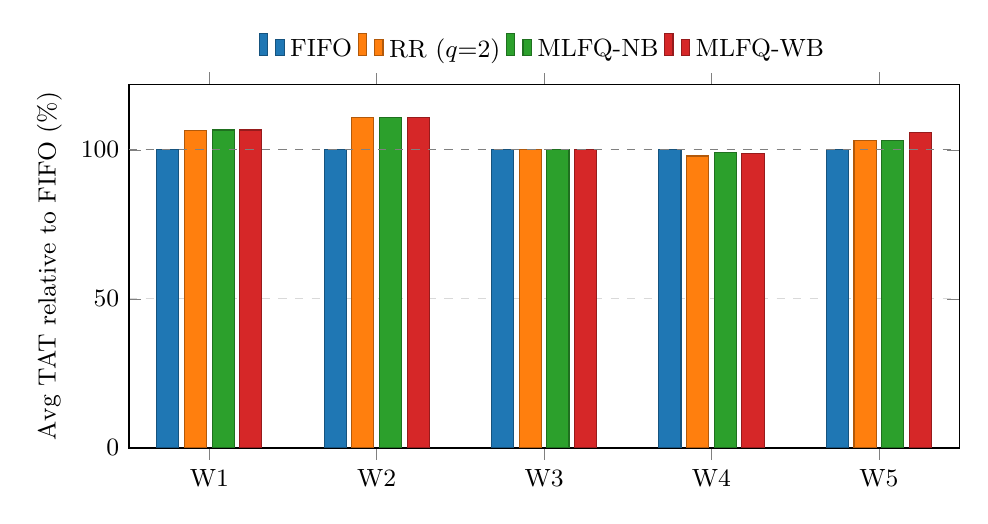
\begin{tikzpicture}
\begin{axis}[barstyle, ylabel={Avg TAT relative to FIFO (\%)}, ymin=0]
\addplot[fill=cFIFO,draw=cFIFO!70!black] coordinates {(W1,100.00) (W2,100.00) (W3,100.00) (W4,100.00) (W5,100.00)};
\addplot[fill=cRR,draw=cRR!70!black] coordinates {(W1,106.38) (W2,110.91) (W3,100.00) (W4,97.95) (W5,103.04)};
\addplot[fill=cNB,draw=cNB!70!black] coordinates {(W1,106.67) (W2,110.91) (W3,100.00) (W4,99.18) (W5,103.20)};
\addplot[fill=cWB,draw=cWB!70!black] coordinates {(W1,106.67) (W2,110.91) (W3,100.00) (W4,98.77) (W5,105.76)};
\draw[dashed,gray] ({rel axis cs:0,0}|-{axis cs:W1,100}) -- ({rel axis cs:1,0}|-{axis cs:W1,100});
\legend{FIFO, RR ($q{=}2$), MLFQ-NB, MLFQ-WB}
\end{axis}\end{tikzpicture}
\caption{Average turnaround time of each algorithm as a percentage of the FIFO result for the same workload, dual processor. Unlike on one processor, FIFO is no longer best everywhere: on workload 4 all three preemptive policies fall below the 100\,\% line.}
\end{figure}
\begin{figure}[htbp]\centering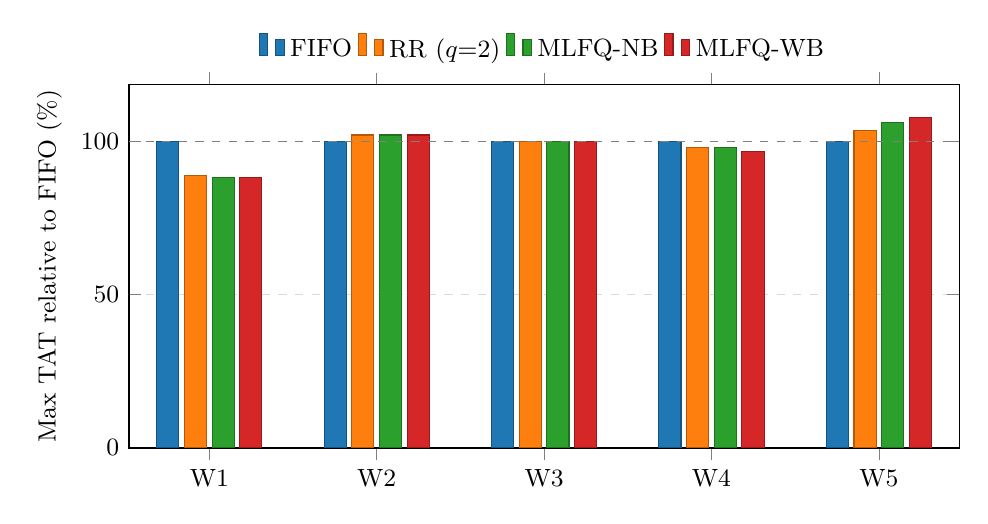
\begin{tikzpicture}
\begin{axis}[barstyle, ylabel={Max TAT relative to FIFO (\%)}, ymin=0]
\addplot[fill=cFIFO,draw=cFIFO!70!black] coordinates {(W1,100.00) (W2,100.00) (W3,100.00) (W4,100.00) (W5,100.00)};
\addplot[fill=cRR,draw=cRR!70!black] coordinates {(W1,88.72) (W2,102.00) (W3,100.00) (W4,97.85) (W5,103.45)};
\addplot[fill=cNB,draw=cNB!70!black] coordinates {(W1,88.21) (W2,102.00) (W3,100.00) (W4,97.85) (W5,106.03)};
\addplot[fill=cWB,draw=cWB!70!black] coordinates {(W1,88.21) (W2,102.00) (W3,100.00) (W4,96.77) (W5,107.76)};
\draw[dashed,gray] ({rel axis cs:0,0}|-{axis cs:W1,100}) -- ({rel axis cs:1,0}|-{axis cs:W1,100});
\legend{FIFO, RR ($q{=}2$), MLFQ-NB, MLFQ-WB}
\end{axis}\end{tikzpicture}
\caption{Maximum (worst-case) turnaround time relative to FIFO, dual processor. The preemptive policies have a lower worst case than FIFO on W1 and W4, and a higher one on W2 and W5.}
\end{figure}
\begin{figure}[htbp]\centering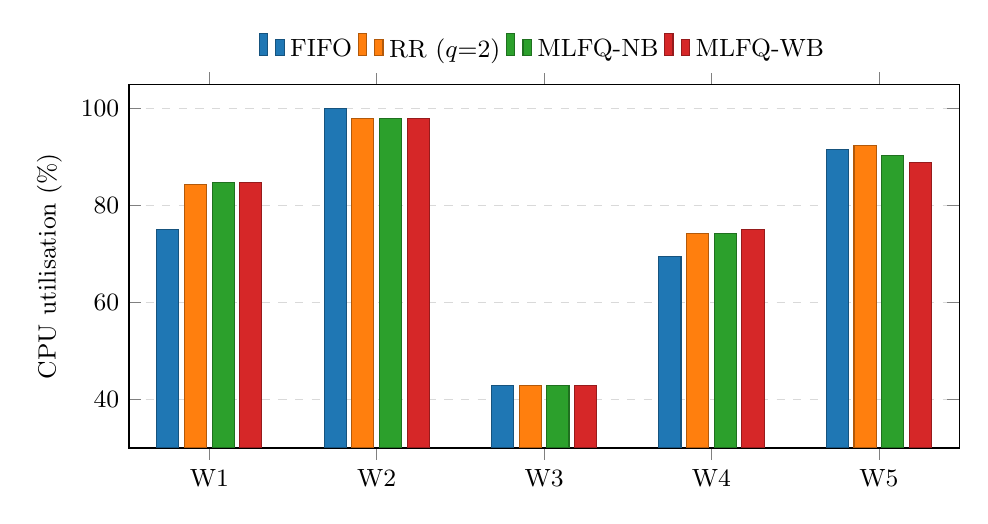
\begin{tikzpicture}
\begin{axis}[barstyle, ylabel={CPU utilisation (\%)}, ymin=30,ymax=105]
\addplot[fill=cFIFO,draw=cFIFO!70!black] coordinates {(W1,75.00) (W2,100.00) (W3,42.86) (W4,69.44) (W5,91.60)};
\addplot[fill=cRR,draw=cRR!70!black] coordinates {(W1,84.27) (W2,98.04) (W3,42.86) (W4,74.26) (W5,92.31)};
\addplot[fill=cNB,draw=cNB!70!black] coordinates {(W1,84.75) (W2,98.04) (W3,42.86) (W4,74.26) (W5,90.23)};
\addplot[fill=cWB,draw=cWB!70!black] coordinates {(W1,84.75) (W2,98.04) (W3,42.86) (W4,75.00) (W5,88.89)};
\legend{FIFO, RR ($q{=}2$), MLFQ-NB, MLFQ-WB}
\end{axis}\end{tikzpicture}
\caption{Utilisation of the pair of processors, i.e.\ total run time divided by $2\times$ makespan. Workload 3 keeps the processors busy less than half the time, because it is limited by I/O rather than by processor capacity.}
\end{figure}
\begin{figure}[htbp]\centering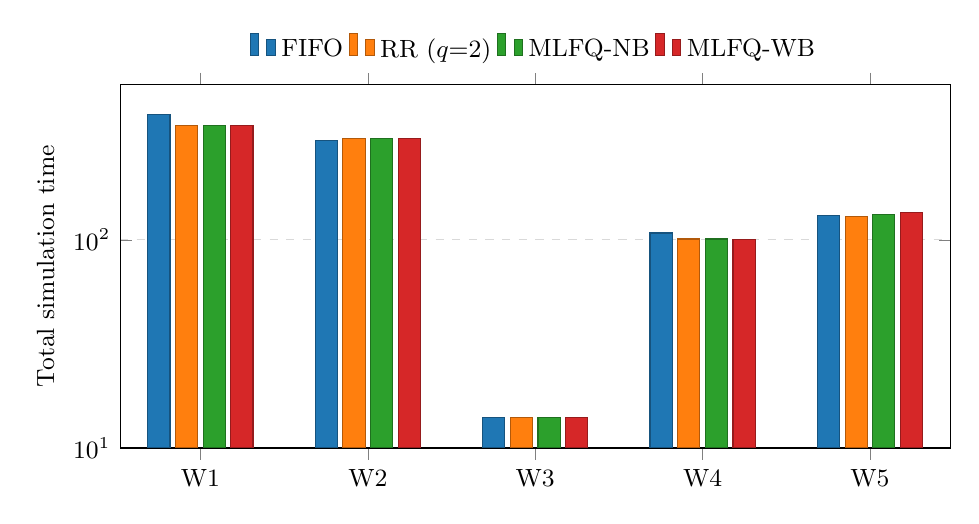
\begin{tikzpicture}
\begin{axis}[barstyle, ylabel={Total simulation time}, ymode=log,log origin=infty]
\addplot[fill=cFIFO,draw=cFIFO!70!black] coordinates {(W1,400.00) (W2,300.00) (W3,14.00) (W4,108.00) (W5,131.00)};
\addplot[fill=cRR,draw=cRR!70!black] coordinates {(W1,356.00) (W2,306.00) (W3,14.00) (W4,101.00) (W5,130.00)};
\addplot[fill=cNB,draw=cNB!70!black] coordinates {(W1,354.00) (W2,306.00) (W3,14.00) (W4,101.00) (W5,133.00)};
\addplot[fill=cWB,draw=cWB!70!black] coordinates {(W1,354.00) (W2,306.00) (W3,14.00) (W4,100.00) (W5,135.00)};
\legend{FIFO, RR ($q{=}2$), MLFQ-NB, MLFQ-WB}
\end{axis}\end{tikzpicture}
\caption{Makespan (total simulation time), dual processor. Lower is better. FIFO has the longest makespan on W1 and W4.}
\end{figure}
\begin{figure}[htbp]\centering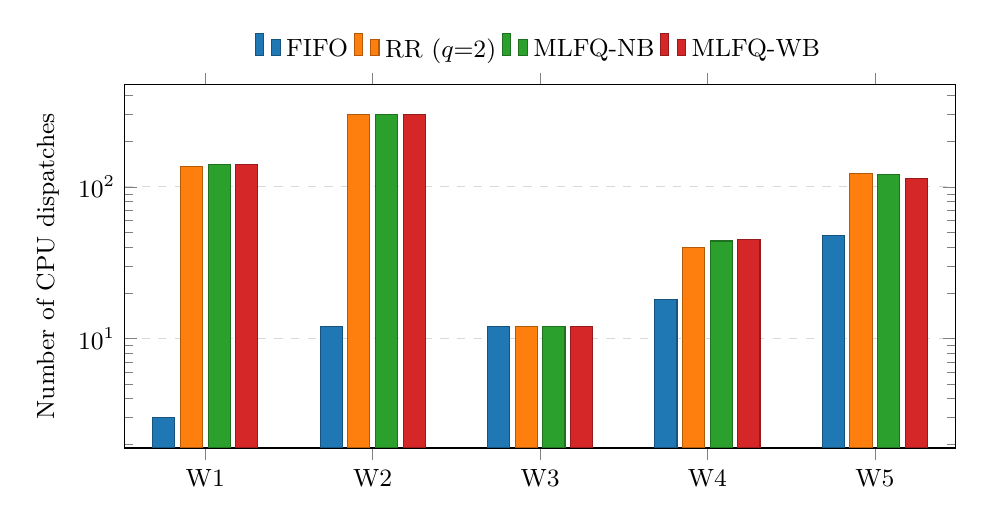
\begin{tikzpicture}
\begin{axis}[barstyle, ylabel={Number of CPU dispatches}, ymode=log,log origin=infty]
\addplot[fill=cFIFO,draw=cFIFO!70!black] coordinates {(W1,3.00) (W2,12.00) (W3,12.00) (W4,18.00) (W5,48.00)};
\addplot[fill=cRR,draw=cRR!70!black] coordinates {(W1,136.00) (W2,300.00) (W3,12.00) (W4,40.00) (W5,123.00)};
\addplot[fill=cNB,draw=cNB!70!black] coordinates {(W1,140.00) (W2,300.00) (W3,12.00) (W4,44.00) (W5,120.00)};
\addplot[fill=cWB,draw=cWB!70!black] coordinates {(W1,140.00) (W2,300.00) (W3,12.00) (W4,45.00) (W5,113.00)};
\legend{FIFO, RR ($q{=}2$), MLFQ-NB, MLFQ-WB}
\end{axis}\end{tikzpicture}
\caption{Number of contiguous CPU segments over both processors, dual processor. FIFO again needs the fewest on every workload.}
\end{figure}
\subsection{Per-process turnaround time}

The aggregate averages hide how differently the policies treat \emph{individual}
processes. The following five charts break the turnaround time down per process, for
every workload.

\begin{figure}[htbp]\centering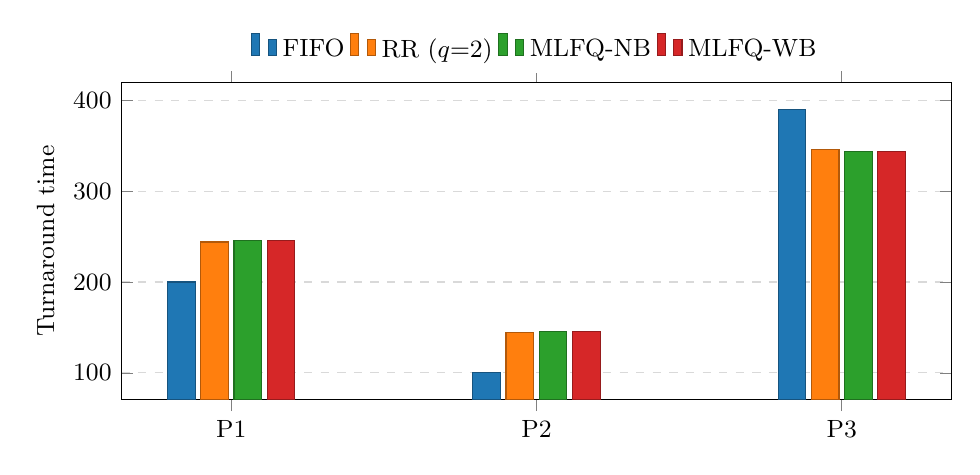
\begin{tikzpicture}
\begin{axis}[ybar,width=\textwidth,height=5.6cm,symbolic x coords={P1,P2,P3},xtick=data,
  enlarge x limits=0.18, ylabel={Turnaround time}, ymajorgrids, grid style={dashed,gray!30},
  legend style={at={(0.5,1.03)},anchor=south,legend columns=4,draw=none,font=\small},
  bar width=10pt, tick label style={font=\small}, label style={font=\small}]
\addplot[fill=cFIFO,draw=cFIFO!70!black] coordinates {(P1,200) (P2,100) (P3,390)};
\addplot[fill=cRR,draw=cRR!70!black] coordinates {(P1,244) (P2,144) (P3,346)};
\addplot[fill=cNB,draw=cNB!70!black] coordinates {(P1,246) (P2,146) (P3,344)};
\addplot[fill=cWB,draw=cWB!70!black] coordinates {(P1,246) (P2,146) (P3,344)};
\legend{FIFO, RR ($q{=}2$), MLFQ-NB, MLFQ-WB}
\end{axis}\end{tikzpicture}
\caption{Per-process turnaround time, workload 1, dual processor. Three pure CPU-bound processes and no I/O at all.}
\end{figure}
\begin{figure}[htbp]\centering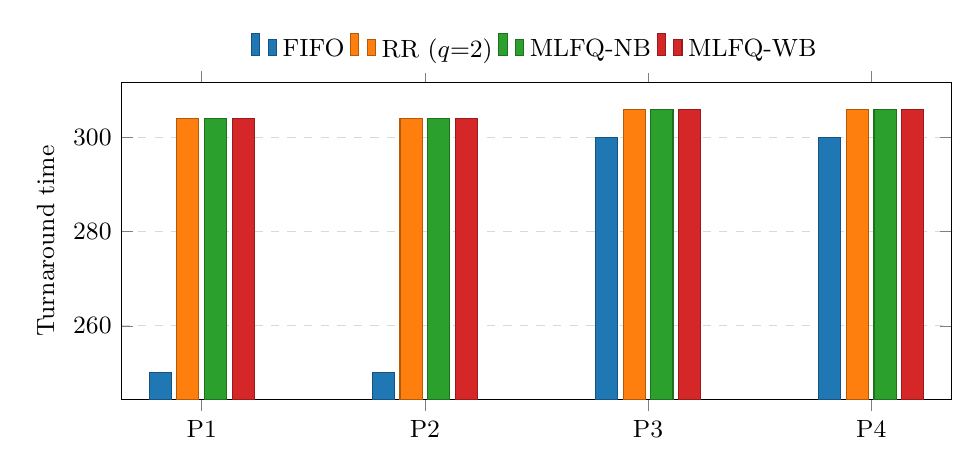
\begin{tikzpicture}
\begin{axis}[ybar,width=\textwidth,height=5.6cm,symbolic x coords={P1,P2,P3,P4},xtick=data,
  enlarge x limits=0.12, ylabel={Turnaround time}, ymajorgrids, grid style={dashed,gray!30},
  legend style={at={(0.5,1.03)},anchor=south,legend columns=4,draw=none,font=\small},
  bar width=8pt, tick label style={font=\small}, label style={font=\small}]
\addplot[fill=cFIFO,draw=cFIFO!70!black] coordinates {(P1,250) (P2,250) (P3,300) (P4,300)};
\addplot[fill=cRR,draw=cRR!70!black] coordinates {(P1,304) (P2,304) (P3,306) (P4,306)};
\addplot[fill=cNB,draw=cNB!70!black] coordinates {(P1,304) (P2,304) (P3,306) (P4,306)};
\addplot[fill=cWB,draw=cWB!70!black] coordinates {(P1,304) (P2,304) (P3,306) (P4,306)};
\legend{FIFO, RR ($q{=}2$), MLFQ-NB, MLFQ-WB}
\end{axis}\end{tikzpicture}
\caption{Per-process turnaround time, workload 2, dual processor. Four identical processes with long (50-unit) CPU bursts.}
\end{figure}
\begin{figure}[htbp]\centering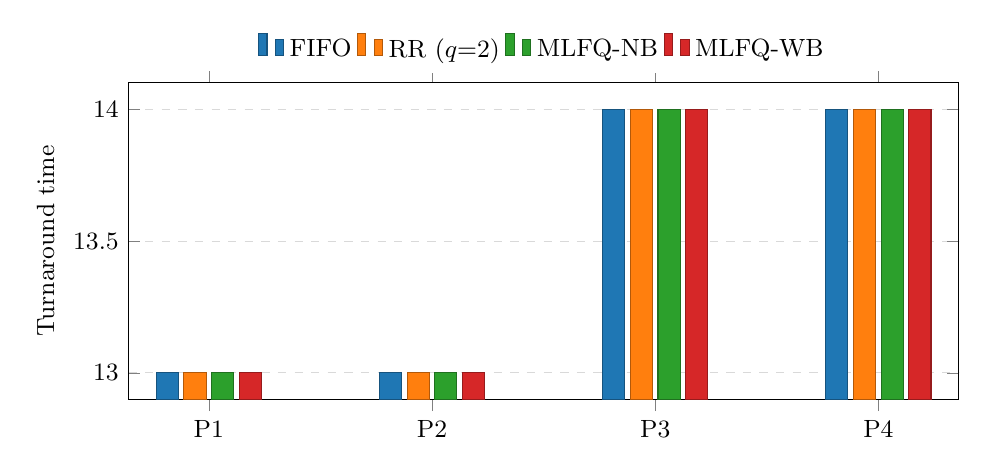
\begin{tikzpicture}
\begin{axis}[ybar,width=\textwidth,height=5.6cm,symbolic x coords={P1,P2,P3,P4},xtick=data,
  enlarge x limits=0.12, ylabel={Turnaround time}, ymajorgrids, grid style={dashed,gray!30},
  legend style={at={(0.5,1.03)},anchor=south,legend columns=4,draw=none,font=\small},
  bar width=8pt, tick label style={font=\small}, label style={font=\small}]
\addplot[fill=cFIFO,draw=cFIFO!70!black] coordinates {(P1,13) (P2,13) (P3,14) (P4,14)};
\addplot[fill=cRR,draw=cRR!70!black] coordinates {(P1,13) (P2,13) (P3,14) (P4,14)};
\addplot[fill=cNB,draw=cNB!70!black] coordinates {(P1,13) (P2,13) (P3,14) (P4,14)};
\addplot[fill=cWB,draw=cWB!70!black] coordinates {(P1,13) (P2,13) (P3,14) (P4,14)};
\legend{FIFO, RR ($q{=}2$), MLFQ-NB, MLFQ-WB}
\end{axis}\end{tikzpicture}
\caption{Per-process turnaround time, workload 3, dual processor. Four identical processes whose CPU bursts are all 1 unit long.}
\end{figure}
\begin{figure}[htbp]\centering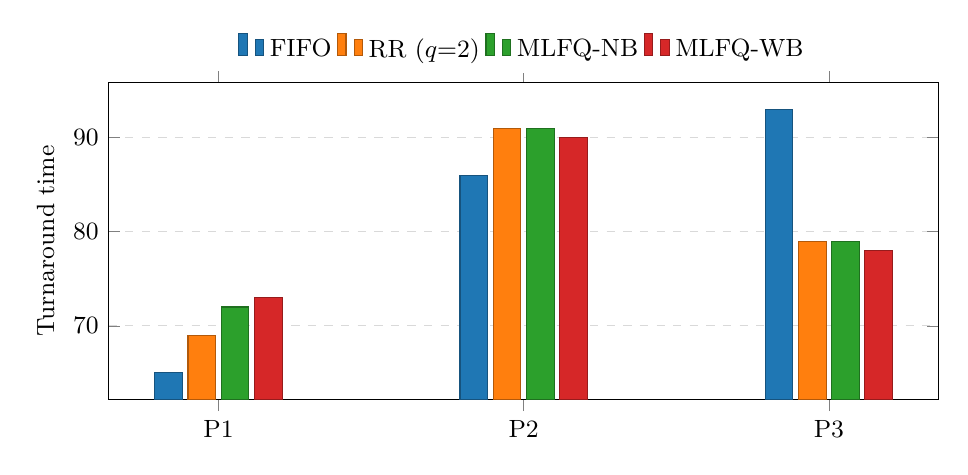
\begin{tikzpicture}
\begin{axis}[ybar,width=\textwidth,height=5.6cm,symbolic x coords={P1,P2,P3},xtick=data,
  enlarge x limits=0.18, ylabel={Turnaround time}, ymajorgrids, grid style={dashed,gray!30},
  legend style={at={(0.5,1.03)},anchor=south,legend columns=4,draw=none,font=\small},
  bar width=10pt, tick label style={font=\small}, label style={font=\small}]
\addplot[fill=cFIFO,draw=cFIFO!70!black] coordinates {(P1,65) (P2,86) (P3,93)};
\addplot[fill=cRR,draw=cRR!70!black] coordinates {(P1,69) (P2,91) (P3,79)};
\addplot[fill=cNB,draw=cNB!70!black] coordinates {(P1,72) (P2,91) (P3,79)};
\addplot[fill=cWB,draw=cWB!70!black] coordinates {(P1,73) (P2,90) (P3,78)};
\legend{FIFO, RR ($q{=}2$), MLFQ-NB, MLFQ-WB}
\end{axis}\end{tikzpicture}
\caption{Per-process turnaround time, workload 4, dual processor. P1 long CPU-bound, P2 medium, P3 short interactive.}
\end{figure}
\begin{figure}[htbp]\centering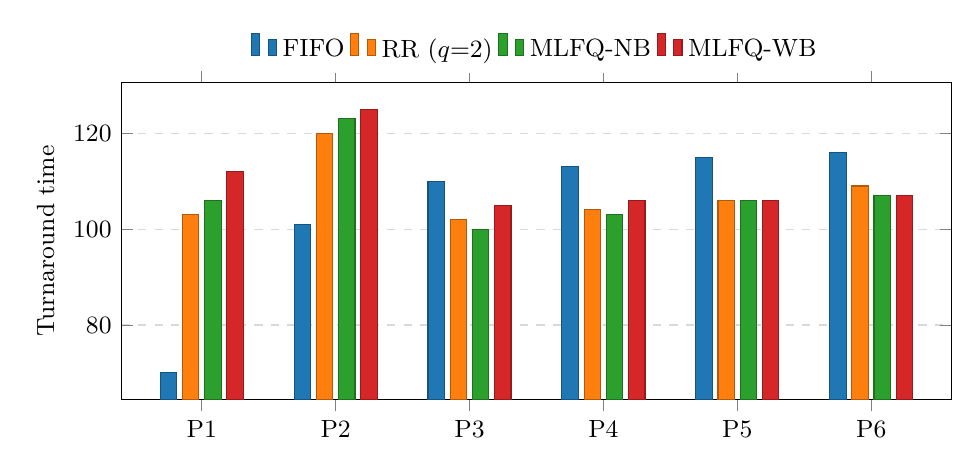
\begin{tikzpicture}
\begin{axis}[ybar,width=\textwidth,height=5.6cm,symbolic x coords={P1,P2,P3,P4,P5,P6},xtick=data,
  enlarge x limits=0.12, ylabel={Turnaround time}, ymajorgrids, grid style={dashed,gray!30},
  legend style={at={(0.5,1.03)},anchor=south,legend columns=4,draw=none,font=\small},
  bar width=6pt, tick label style={font=\small}, label style={font=\small}]
\addplot[fill=cFIFO,draw=cFIFO!70!black] coordinates {(P1,70) (P2,101) (P3,110) (P4,113) (P5,115) (P6,116)};
\addplot[fill=cRR,draw=cRR!70!black] coordinates {(P1,103) (P2,120) (P3,102) (P4,104) (P5,106) (P6,109)};
\addplot[fill=cNB,draw=cNB!70!black] coordinates {(P1,106) (P2,123) (P3,100) (P4,103) (P5,106) (P6,107)};
\addplot[fill=cWB,draw=cWB!70!black] coordinates {(P1,112) (P2,125) (P3,105) (P4,106) (P5,106) (P6,107)};
\legend{FIFO, RR ($q{=}2$), MLFQ-NB, MLFQ-WB}
\end{axis}\end{tikzpicture}
\caption{Per-process turnaround time, workload 5, dual processor. P1 long, P2 medium, P3--P6 short interactive, all arriving at $t=15$.}
\end{figure}
\clearpage
\subsection{Schedule visualisation (Gantt charts)}
The charts below show the complete dual-processor schedules. As in Part I each row is a
process, but the \emph{colour} of each block now shows which processor ran it: blue for
CPU0 and orange for CPU1. A row that changes colour part-way through a burst is a process
that migrated between processors. The heading of each chart gives the makespan, the idle
time summed over both processors, and the number of migrated bursts.

\begin{figure}[H]\centering
{\small\tikz{\fill[cCPU0] (0,0) rectangle (0.35,0.22);}~CPU0\qquad\tikz{\fill[cCPU1] (0,0) rectangle (0.35,0.22);}~CPU1}\par
\par\vspace{1.5mm}{\small\textbf{FIFO}\quad(makespan 400, idle 200, 0 bursts migrated)}\par\vspace{0.8mm}
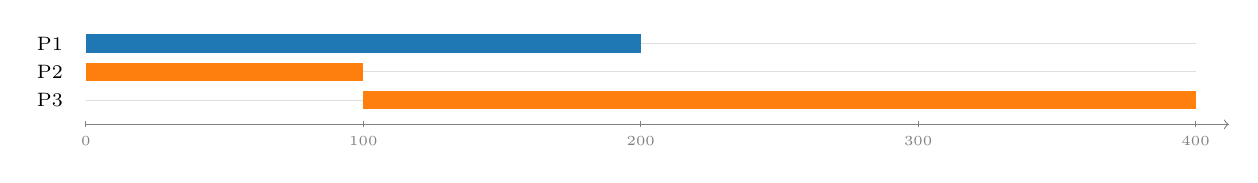
\begin{tikzpicture}[x=0.03524cm,y=0.36cm]
\node[anchor=east,font=\scriptsize] at (-4.8,2) {P1};
\draw[gray!25] (0,2) -- (400,2);
\node[anchor=east,font=\scriptsize] at (-4.8,1) {P2};
\draw[gray!25] (0,1) -- (400,1);
\node[anchor=east,font=\scriptsize] at (-4.8,0) {P3};
\draw[gray!25] (0,0) -- (400,0);
\fill[cCPU0] (0,1.68) rectangle (200,2.32);
\fill[cCPU1] (0,0.68) rectangle (100,1.32);
\fill[cCPU1] (100,-0.32) rectangle (400,0.32);
\draw[->,gray] (0,-0.85) -- (412.0,-0.85);
\draw[gray] (0,-0.75)--(0,-0.95) node[below,font=\tiny]{0};
\draw[gray] (100,-0.75)--(100,-0.95) node[below,font=\tiny]{100};
\draw[gray] (200,-0.75)--(200,-0.95) node[below,font=\tiny]{200};
\draw[gray] (300,-0.75)--(300,-0.95) node[below,font=\tiny]{300};
\draw[gray] (400,-0.75)--(400,-0.95) node[below,font=\tiny]{400};
\end{tikzpicture}\par
\par\vspace{1.5mm}{\small\textbf{RR}\quad(makespan 356, idle 112, 3 bursts migrated)}\par\vspace{0.8mm}
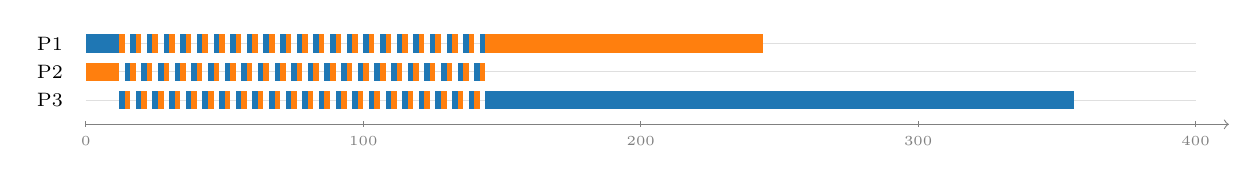
\begin{tikzpicture}[x=0.03524cm,y=0.36cm]
\node[anchor=east,font=\scriptsize] at (-4.8,2) {P1};
\draw[gray!25] (0,2) -- (400,2);
\node[anchor=east,font=\scriptsize] at (-4.8,1) {P2};
\draw[gray!25] (0,1) -- (400,1);
\node[anchor=east,font=\scriptsize] at (-4.8,0) {P3};
\draw[gray!25] (0,0) -- (400,0);
\fill[cCPU0] (0,1.68) rectangle (12,2.32);
\fill[cCPU0] (12,-0.32) rectangle (14,0.32);
\fill[cCPU0] (14,0.68) rectangle (16,1.32);
\fill[cCPU0] (16,1.68) rectangle (18,2.32);
\fill[cCPU0] (18,-0.32) rectangle (20,0.32);
\fill[cCPU0] (20,0.68) rectangle (22,1.32);
\fill[cCPU0] (22,1.68) rectangle (24,2.32);
\fill[cCPU0] (24,-0.32) rectangle (26,0.32);
\fill[cCPU0] (26,0.68) rectangle (28,1.32);
\fill[cCPU0] (28,1.68) rectangle (30,2.32);
\fill[cCPU0] (30,-0.32) rectangle (32,0.32);
\fill[cCPU0] (32,0.68) rectangle (34,1.32);
\fill[cCPU0] (34,1.68) rectangle (36,2.32);
\fill[cCPU0] (36,-0.32) rectangle (38,0.32);
\fill[cCPU0] (38,0.68) rectangle (40,1.32);
\fill[cCPU0] (40,1.68) rectangle (42,2.32);
\fill[cCPU0] (42,-0.32) rectangle (44,0.32);
\fill[cCPU0] (44,0.68) rectangle (46,1.32);
\fill[cCPU0] (46,1.68) rectangle (48,2.32);
\fill[cCPU0] (48,-0.32) rectangle (50,0.32);
\fill[cCPU0] (50,0.68) rectangle (52,1.32);
\fill[cCPU0] (52,1.68) rectangle (54,2.32);
\fill[cCPU0] (54,-0.32) rectangle (56,0.32);
\fill[cCPU0] (56,0.68) rectangle (58,1.32);
\fill[cCPU0] (58,1.68) rectangle (60,2.32);
\fill[cCPU0] (60,-0.32) rectangle (62,0.32);
\fill[cCPU0] (62,0.68) rectangle (64,1.32);
\fill[cCPU0] (64,1.68) rectangle (66,2.32);
\fill[cCPU0] (66,-0.32) rectangle (68,0.32);
\fill[cCPU0] (68,0.68) rectangle (70,1.32);
\fill[cCPU0] (70,1.68) rectangle (72,2.32);
\fill[cCPU0] (72,-0.32) rectangle (74,0.32);
\fill[cCPU0] (74,0.68) rectangle (76,1.32);
\fill[cCPU0] (76,1.68) rectangle (78,2.32);
\fill[cCPU0] (78,-0.32) rectangle (80,0.32);
\fill[cCPU0] (80,0.68) rectangle (82,1.32);
\fill[cCPU0] (82,1.68) rectangle (84,2.32);
\fill[cCPU0] (84,-0.32) rectangle (86,0.32);
\fill[cCPU0] (86,0.68) rectangle (88,1.32);
\fill[cCPU0] (88,1.68) rectangle (90,2.32);
\fill[cCPU0] (90,-0.32) rectangle (92,0.32);
\fill[cCPU0] (92,0.68) rectangle (94,1.32);
\fill[cCPU0] (94,1.68) rectangle (96,2.32);
\fill[cCPU0] (96,-0.32) rectangle (98,0.32);
\fill[cCPU0] (98,0.68) rectangle (100,1.32);
\fill[cCPU0] (100,1.68) rectangle (102,2.32);
\fill[cCPU0] (102,-0.32) rectangle (104,0.32);
\fill[cCPU0] (104,0.68) rectangle (106,1.32);
\fill[cCPU0] (106,1.68) rectangle (108,2.32);
\fill[cCPU0] (108,-0.32) rectangle (110,0.32);
\fill[cCPU0] (110,0.68) rectangle (112,1.32);
\fill[cCPU0] (112,1.68) rectangle (114,2.32);
\fill[cCPU0] (114,-0.32) rectangle (116,0.32);
\fill[cCPU0] (116,0.68) rectangle (118,1.32);
\fill[cCPU0] (118,1.68) rectangle (120,2.32);
\fill[cCPU0] (120,-0.32) rectangle (122,0.32);
\fill[cCPU0] (122,0.68) rectangle (124,1.32);
\fill[cCPU0] (124,1.68) rectangle (126,2.32);
\fill[cCPU0] (126,-0.32) rectangle (128,0.32);
\fill[cCPU0] (128,0.68) rectangle (130,1.32);
\fill[cCPU0] (130,1.68) rectangle (132,2.32);
\fill[cCPU0] (132,-0.32) rectangle (134,0.32);
\fill[cCPU0] (134,0.68) rectangle (136,1.32);
\fill[cCPU0] (136,1.68) rectangle (138,2.32);
\fill[cCPU0] (138,-0.32) rectangle (140,0.32);
\fill[cCPU0] (140,0.68) rectangle (142,1.32);
\fill[cCPU0] (142,1.68) rectangle (144,2.32);
\fill[cCPU0] (144,-0.32) rectangle (356,0.32);
\fill[cCPU1] (0,0.68) rectangle (12,1.32);
\fill[cCPU1] (12,1.68) rectangle (14,2.32);
\fill[cCPU1] (14,-0.32) rectangle (16,0.32);
\fill[cCPU1] (16,0.68) rectangle (18,1.32);
\fill[cCPU1] (18,1.68) rectangle (20,2.32);
\fill[cCPU1] (20,-0.32) rectangle (22,0.32);
\fill[cCPU1] (22,0.68) rectangle (24,1.32);
\fill[cCPU1] (24,1.68) rectangle (26,2.32);
\fill[cCPU1] (26,-0.32) rectangle (28,0.32);
\fill[cCPU1] (28,0.68) rectangle (30,1.32);
\fill[cCPU1] (30,1.68) rectangle (32,2.32);
\fill[cCPU1] (32,-0.32) rectangle (34,0.32);
\fill[cCPU1] (34,0.68) rectangle (36,1.32);
\fill[cCPU1] (36,1.68) rectangle (38,2.32);
\fill[cCPU1] (38,-0.32) rectangle (40,0.32);
\fill[cCPU1] (40,0.68) rectangle (42,1.32);
\fill[cCPU1] (42,1.68) rectangle (44,2.32);
\fill[cCPU1] (44,-0.32) rectangle (46,0.32);
\fill[cCPU1] (46,0.68) rectangle (48,1.32);
\fill[cCPU1] (48,1.68) rectangle (50,2.32);
\fill[cCPU1] (50,-0.32) rectangle (52,0.32);
\fill[cCPU1] (52,0.68) rectangle (54,1.32);
\fill[cCPU1] (54,1.68) rectangle (56,2.32);
\fill[cCPU1] (56,-0.32) rectangle (58,0.32);
\fill[cCPU1] (58,0.68) rectangle (60,1.32);
\fill[cCPU1] (60,1.68) rectangle (62,2.32);
\fill[cCPU1] (62,-0.32) rectangle (64,0.32);
\fill[cCPU1] (64,0.68) rectangle (66,1.32);
\fill[cCPU1] (66,1.68) rectangle (68,2.32);
\fill[cCPU1] (68,-0.32) rectangle (70,0.32);
\fill[cCPU1] (70,0.68) rectangle (72,1.32);
\fill[cCPU1] (72,1.68) rectangle (74,2.32);
\fill[cCPU1] (74,-0.32) rectangle (76,0.32);
\fill[cCPU1] (76,0.68) rectangle (78,1.32);
\fill[cCPU1] (78,1.68) rectangle (80,2.32);
\fill[cCPU1] (80,-0.32) rectangle (82,0.32);
\fill[cCPU1] (82,0.68) rectangle (84,1.32);
\fill[cCPU1] (84,1.68) rectangle (86,2.32);
\fill[cCPU1] (86,-0.32) rectangle (88,0.32);
\fill[cCPU1] (88,0.68) rectangle (90,1.32);
\fill[cCPU1] (90,1.68) rectangle (92,2.32);
\fill[cCPU1] (92,-0.32) rectangle (94,0.32);
\fill[cCPU1] (94,0.68) rectangle (96,1.32);
\fill[cCPU1] (96,1.68) rectangle (98,2.32);
\fill[cCPU1] (98,-0.32) rectangle (100,0.32);
\fill[cCPU1] (100,0.68) rectangle (102,1.32);
\fill[cCPU1] (102,1.68) rectangle (104,2.32);
\fill[cCPU1] (104,-0.32) rectangle (106,0.32);
\fill[cCPU1] (106,0.68) rectangle (108,1.32);
\fill[cCPU1] (108,1.68) rectangle (110,2.32);
\fill[cCPU1] (110,-0.32) rectangle (112,0.32);
\fill[cCPU1] (112,0.68) rectangle (114,1.32);
\fill[cCPU1] (114,1.68) rectangle (116,2.32);
\fill[cCPU1] (116,-0.32) rectangle (118,0.32);
\fill[cCPU1] (118,0.68) rectangle (120,1.32);
\fill[cCPU1] (120,1.68) rectangle (122,2.32);
\fill[cCPU1] (122,-0.32) rectangle (124,0.32);
\fill[cCPU1] (124,0.68) rectangle (126,1.32);
\fill[cCPU1] (126,1.68) rectangle (128,2.32);
\fill[cCPU1] (128,-0.32) rectangle (130,0.32);
\fill[cCPU1] (130,0.68) rectangle (132,1.32);
\fill[cCPU1] (132,1.68) rectangle (134,2.32);
\fill[cCPU1] (134,-0.32) rectangle (136,0.32);
\fill[cCPU1] (136,0.68) rectangle (138,1.32);
\fill[cCPU1] (138,1.68) rectangle (140,2.32);
\fill[cCPU1] (140,-0.32) rectangle (142,0.32);
\fill[cCPU1] (142,0.68) rectangle (144,1.32);
\fill[cCPU1] (144,1.68) rectangle (244,2.32);
\draw[->,gray] (0,-0.85) -- (412.0,-0.85);
\draw[gray] (0,-0.75)--(0,-0.95) node[below,font=\tiny]{0};
\draw[gray] (100,-0.75)--(100,-0.95) node[below,font=\tiny]{100};
\draw[gray] (200,-0.75)--(200,-0.95) node[below,font=\tiny]{200};
\draw[gray] (300,-0.75)--(300,-0.95) node[below,font=\tiny]{300};
\draw[gray] (400,-0.75)--(400,-0.95) node[below,font=\tiny]{400};
\end{tikzpicture}\par
\par\vspace{1.5mm}{\small\textbf{MLFQ-NB}\quad(makespan 354, idle 108, 3 bursts migrated)}\par\vspace{0.8mm}
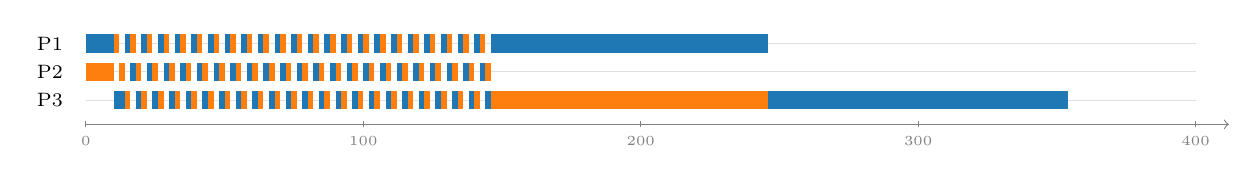
\begin{tikzpicture}[x=0.03524cm,y=0.36cm]
\node[anchor=east,font=\scriptsize] at (-4.8,2) {P1};
\draw[gray!25] (0,2) -- (400,2);
\node[anchor=east,font=\scriptsize] at (-4.8,1) {P2};
\draw[gray!25] (0,1) -- (400,1);
\node[anchor=east,font=\scriptsize] at (-4.8,0) {P3};
\draw[gray!25] (0,0) -- (400,0);
\fill[cCPU0] (0,1.68) rectangle (10,2.32);
\fill[cCPU0] (10,-0.32) rectangle (14,0.32);
\fill[cCPU0] (14,1.68) rectangle (16,2.32);
\fill[cCPU0] (16,0.68) rectangle (18,1.32);
\fill[cCPU0] (18,-0.32) rectangle (20,0.32);
\fill[cCPU0] (20,1.68) rectangle (22,2.32);
\fill[cCPU0] (22,0.68) rectangle (24,1.32);
\fill[cCPU0] (24,-0.32) rectangle (26,0.32);
\fill[cCPU0] (26,1.68) rectangle (28,2.32);
\fill[cCPU0] (28,0.68) rectangle (30,1.32);
\fill[cCPU0] (30,-0.32) rectangle (32,0.32);
\fill[cCPU0] (32,1.68) rectangle (34,2.32);
\fill[cCPU0] (34,0.68) rectangle (36,1.32);
\fill[cCPU0] (36,-0.32) rectangle (38,0.32);
\fill[cCPU0] (38,1.68) rectangle (40,2.32);
\fill[cCPU0] (40,0.68) rectangle (42,1.32);
\fill[cCPU0] (42,-0.32) rectangle (44,0.32);
\fill[cCPU0] (44,1.68) rectangle (46,2.32);
\fill[cCPU0] (46,0.68) rectangle (48,1.32);
\fill[cCPU0] (48,-0.32) rectangle (50,0.32);
\fill[cCPU0] (50,1.68) rectangle (52,2.32);
\fill[cCPU0] (52,0.68) rectangle (54,1.32);
\fill[cCPU0] (54,-0.32) rectangle (56,0.32);
\fill[cCPU0] (56,1.68) rectangle (58,2.32);
\fill[cCPU0] (58,0.68) rectangle (60,1.32);
\fill[cCPU0] (60,-0.32) rectangle (62,0.32);
\fill[cCPU0] (62,1.68) rectangle (64,2.32);
\fill[cCPU0] (64,0.68) rectangle (66,1.32);
\fill[cCPU0] (66,-0.32) rectangle (68,0.32);
\fill[cCPU0] (68,1.68) rectangle (70,2.32);
\fill[cCPU0] (70,0.68) rectangle (72,1.32);
\fill[cCPU0] (72,-0.32) rectangle (74,0.32);
\fill[cCPU0] (74,1.68) rectangle (76,2.32);
\fill[cCPU0] (76,0.68) rectangle (78,1.32);
\fill[cCPU0] (78,-0.32) rectangle (80,0.32);
\fill[cCPU0] (80,1.68) rectangle (82,2.32);
\fill[cCPU0] (82,0.68) rectangle (84,1.32);
\fill[cCPU0] (84,-0.32) rectangle (86,0.32);
\fill[cCPU0] (86,1.68) rectangle (88,2.32);
\fill[cCPU0] (88,0.68) rectangle (90,1.32);
\fill[cCPU0] (90,-0.32) rectangle (92,0.32);
\fill[cCPU0] (92,1.68) rectangle (94,2.32);
\fill[cCPU0] (94,0.68) rectangle (96,1.32);
\fill[cCPU0] (96,-0.32) rectangle (98,0.32);
\fill[cCPU0] (98,1.68) rectangle (100,2.32);
\fill[cCPU0] (100,0.68) rectangle (102,1.32);
\fill[cCPU0] (102,-0.32) rectangle (104,0.32);
\fill[cCPU0] (104,1.68) rectangle (106,2.32);
\fill[cCPU0] (106,0.68) rectangle (108,1.32);
\fill[cCPU0] (108,-0.32) rectangle (110,0.32);
\fill[cCPU0] (110,1.68) rectangle (112,2.32);
\fill[cCPU0] (112,0.68) rectangle (114,1.32);
\fill[cCPU0] (114,-0.32) rectangle (116,0.32);
\fill[cCPU0] (116,1.68) rectangle (118,2.32);
\fill[cCPU0] (118,0.68) rectangle (120,1.32);
\fill[cCPU0] (120,-0.32) rectangle (122,0.32);
\fill[cCPU0] (122,1.68) rectangle (124,2.32);
\fill[cCPU0] (124,0.68) rectangle (126,1.32);
\fill[cCPU0] (126,-0.32) rectangle (128,0.32);
\fill[cCPU0] (128,1.68) rectangle (130,2.32);
\fill[cCPU0] (130,0.68) rectangle (132,1.32);
\fill[cCPU0] (132,-0.32) rectangle (134,0.32);
\fill[cCPU0] (134,1.68) rectangle (136,2.32);
\fill[cCPU0] (136,0.68) rectangle (138,1.32);
\fill[cCPU0] (138,-0.32) rectangle (140,0.32);
\fill[cCPU0] (140,1.68) rectangle (142,2.32);
\fill[cCPU0] (142,0.68) rectangle (144,1.32);
\fill[cCPU0] (144,-0.32) rectangle (146,0.32);
\fill[cCPU0] (146,1.68) rectangle (246,2.32);
\fill[cCPU0] (246,-0.32) rectangle (354,0.32);
\fill[cCPU1] (0,0.68) rectangle (10,1.32);
\fill[cCPU1] (10,1.68) rectangle (12,2.32);
\fill[cCPU1] (12,0.68) rectangle (14,1.32);
\fill[cCPU1] (14,-0.32) rectangle (16,0.32);
\fill[cCPU1] (16,1.68) rectangle (18,2.32);
\fill[cCPU1] (18,0.68) rectangle (20,1.32);
\fill[cCPU1] (20,-0.32) rectangle (22,0.32);
\fill[cCPU1] (22,1.68) rectangle (24,2.32);
\fill[cCPU1] (24,0.68) rectangle (26,1.32);
\fill[cCPU1] (26,-0.32) rectangle (28,0.32);
\fill[cCPU1] (28,1.68) rectangle (30,2.32);
\fill[cCPU1] (30,0.68) rectangle (32,1.32);
\fill[cCPU1] (32,-0.32) rectangle (34,0.32);
\fill[cCPU1] (34,1.68) rectangle (36,2.32);
\fill[cCPU1] (36,0.68) rectangle (38,1.32);
\fill[cCPU1] (38,-0.32) rectangle (40,0.32);
\fill[cCPU1] (40,1.68) rectangle (42,2.32);
\fill[cCPU1] (42,0.68) rectangle (44,1.32);
\fill[cCPU1] (44,-0.32) rectangle (46,0.32);
\fill[cCPU1] (46,1.68) rectangle (48,2.32);
\fill[cCPU1] (48,0.68) rectangle (50,1.32);
\fill[cCPU1] (50,-0.32) rectangle (52,0.32);
\fill[cCPU1] (52,1.68) rectangle (54,2.32);
\fill[cCPU1] (54,0.68) rectangle (56,1.32);
\fill[cCPU1] (56,-0.32) rectangle (58,0.32);
\fill[cCPU1] (58,1.68) rectangle (60,2.32);
\fill[cCPU1] (60,0.68) rectangle (62,1.32);
\fill[cCPU1] (62,-0.32) rectangle (64,0.32);
\fill[cCPU1] (64,1.68) rectangle (66,2.32);
\fill[cCPU1] (66,0.68) rectangle (68,1.32);
\fill[cCPU1] (68,-0.32) rectangle (70,0.32);
\fill[cCPU1] (70,1.68) rectangle (72,2.32);
\fill[cCPU1] (72,0.68) rectangle (74,1.32);
\fill[cCPU1] (74,-0.32) rectangle (76,0.32);
\fill[cCPU1] (76,1.68) rectangle (78,2.32);
\fill[cCPU1] (78,0.68) rectangle (80,1.32);
\fill[cCPU1] (80,-0.32) rectangle (82,0.32);
\fill[cCPU1] (82,1.68) rectangle (84,2.32);
\fill[cCPU1] (84,0.68) rectangle (86,1.32);
\fill[cCPU1] (86,-0.32) rectangle (88,0.32);
\fill[cCPU1] (88,1.68) rectangle (90,2.32);
\fill[cCPU1] (90,0.68) rectangle (92,1.32);
\fill[cCPU1] (92,-0.32) rectangle (94,0.32);
\fill[cCPU1] (94,1.68) rectangle (96,2.32);
\fill[cCPU1] (96,0.68) rectangle (98,1.32);
\fill[cCPU1] (98,-0.32) rectangle (100,0.32);
\fill[cCPU1] (100,1.68) rectangle (102,2.32);
\fill[cCPU1] (102,0.68) rectangle (104,1.32);
\fill[cCPU1] (104,-0.32) rectangle (106,0.32);
\fill[cCPU1] (106,1.68) rectangle (108,2.32);
\fill[cCPU1] (108,0.68) rectangle (110,1.32);
\fill[cCPU1] (110,-0.32) rectangle (112,0.32);
\fill[cCPU1] (112,1.68) rectangle (114,2.32);
\fill[cCPU1] (114,0.68) rectangle (116,1.32);
\fill[cCPU1] (116,-0.32) rectangle (118,0.32);
\fill[cCPU1] (118,1.68) rectangle (120,2.32);
\fill[cCPU1] (120,0.68) rectangle (122,1.32);
\fill[cCPU1] (122,-0.32) rectangle (124,0.32);
\fill[cCPU1] (124,1.68) rectangle (126,2.32);
\fill[cCPU1] (126,0.68) rectangle (128,1.32);
\fill[cCPU1] (128,-0.32) rectangle (130,0.32);
\fill[cCPU1] (130,1.68) rectangle (132,2.32);
\fill[cCPU1] (132,0.68) rectangle (134,1.32);
\fill[cCPU1] (134,-0.32) rectangle (136,0.32);
\fill[cCPU1] (136,1.68) rectangle (138,2.32);
\fill[cCPU1] (138,0.68) rectangle (140,1.32);
\fill[cCPU1] (140,-0.32) rectangle (142,0.32);
\fill[cCPU1] (142,1.68) rectangle (144,2.32);
\fill[cCPU1] (144,0.68) rectangle (146,1.32);
\fill[cCPU1] (146,-0.32) rectangle (246,0.32);
\draw[->,gray] (0,-0.85) -- (412.0,-0.85);
\draw[gray] (0,-0.75)--(0,-0.95) node[below,font=\tiny]{0};
\draw[gray] (100,-0.75)--(100,-0.95) node[below,font=\tiny]{100};
\draw[gray] (200,-0.75)--(200,-0.95) node[below,font=\tiny]{200};
\draw[gray] (300,-0.75)--(300,-0.95) node[below,font=\tiny]{300};
\draw[gray] (400,-0.75)--(400,-0.95) node[below,font=\tiny]{400};
\end{tikzpicture}\par
\par\vspace{1.5mm}{\small\textbf{MLFQ-WB}\quad(makespan 354, idle 108, 3 bursts migrated)}\par\vspace{0.8mm}
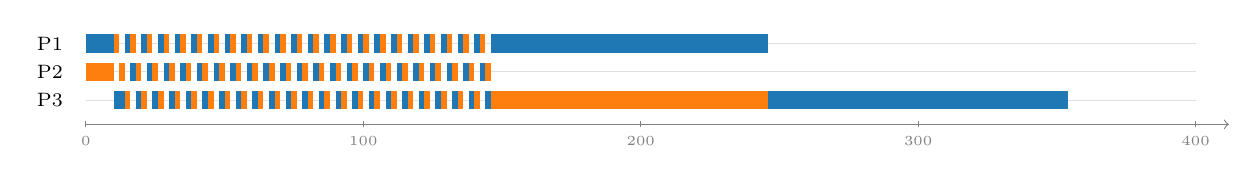
\begin{tikzpicture}[x=0.03524cm,y=0.36cm]
\node[anchor=east,font=\scriptsize] at (-4.8,2) {P1};
\draw[gray!25] (0,2) -- (400,2);
\node[anchor=east,font=\scriptsize] at (-4.8,1) {P2};
\draw[gray!25] (0,1) -- (400,1);
\node[anchor=east,font=\scriptsize] at (-4.8,0) {P3};
\draw[gray!25] (0,0) -- (400,0);
\fill[cCPU0] (0,1.68) rectangle (10,2.32);
\fill[cCPU0] (10,-0.32) rectangle (14,0.32);
\fill[cCPU0] (14,1.68) rectangle (16,2.32);
\fill[cCPU0] (16,0.68) rectangle (18,1.32);
\fill[cCPU0] (18,-0.32) rectangle (20,0.32);
\fill[cCPU0] (20,1.68) rectangle (22,2.32);
\fill[cCPU0] (22,0.68) rectangle (24,1.32);
\fill[cCPU0] (24,-0.32) rectangle (26,0.32);
\fill[cCPU0] (26,1.68) rectangle (28,2.32);
\fill[cCPU0] (28,0.68) rectangle (30,1.32);
\fill[cCPU0] (30,-0.32) rectangle (32,0.32);
\fill[cCPU0] (32,1.68) rectangle (34,2.32);
\fill[cCPU0] (34,0.68) rectangle (36,1.32);
\fill[cCPU0] (36,-0.32) rectangle (38,0.32);
\fill[cCPU0] (38,1.68) rectangle (40,2.32);
\fill[cCPU0] (40,0.68) rectangle (42,1.32);
\fill[cCPU0] (42,-0.32) rectangle (44,0.32);
\fill[cCPU0] (44,1.68) rectangle (46,2.32);
\fill[cCPU0] (46,0.68) rectangle (48,1.32);
\fill[cCPU0] (48,-0.32) rectangle (50,0.32);
\fill[cCPU0] (50,1.68) rectangle (52,2.32);
\fill[cCPU0] (52,0.68) rectangle (54,1.32);
\fill[cCPU0] (54,-0.32) rectangle (56,0.32);
\fill[cCPU0] (56,1.68) rectangle (58,2.32);
\fill[cCPU0] (58,0.68) rectangle (60,1.32);
\fill[cCPU0] (60,-0.32) rectangle (62,0.32);
\fill[cCPU0] (62,1.68) rectangle (64,2.32);
\fill[cCPU0] (64,0.68) rectangle (66,1.32);
\fill[cCPU0] (66,-0.32) rectangle (68,0.32);
\fill[cCPU0] (68,1.68) rectangle (70,2.32);
\fill[cCPU0] (70,0.68) rectangle (72,1.32);
\fill[cCPU0] (72,-0.32) rectangle (74,0.32);
\fill[cCPU0] (74,1.68) rectangle (76,2.32);
\fill[cCPU0] (76,0.68) rectangle (78,1.32);
\fill[cCPU0] (78,-0.32) rectangle (80,0.32);
\fill[cCPU0] (80,1.68) rectangle (82,2.32);
\fill[cCPU0] (82,0.68) rectangle (84,1.32);
\fill[cCPU0] (84,-0.32) rectangle (86,0.32);
\fill[cCPU0] (86,1.68) rectangle (88,2.32);
\fill[cCPU0] (88,0.68) rectangle (90,1.32);
\fill[cCPU0] (90,-0.32) rectangle (92,0.32);
\fill[cCPU0] (92,1.68) rectangle (94,2.32);
\fill[cCPU0] (94,0.68) rectangle (96,1.32);
\fill[cCPU0] (96,-0.32) rectangle (98,0.32);
\fill[cCPU0] (98,1.68) rectangle (100,2.32);
\fill[cCPU0] (100,0.68) rectangle (102,1.32);
\fill[cCPU0] (102,-0.32) rectangle (104,0.32);
\fill[cCPU0] (104,1.68) rectangle (106,2.32);
\fill[cCPU0] (106,0.68) rectangle (108,1.32);
\fill[cCPU0] (108,-0.32) rectangle (110,0.32);
\fill[cCPU0] (110,1.68) rectangle (112,2.32);
\fill[cCPU0] (112,0.68) rectangle (114,1.32);
\fill[cCPU0] (114,-0.32) rectangle (116,0.32);
\fill[cCPU0] (116,1.68) rectangle (118,2.32);
\fill[cCPU0] (118,0.68) rectangle (120,1.32);
\fill[cCPU0] (120,-0.32) rectangle (122,0.32);
\fill[cCPU0] (122,1.68) rectangle (124,2.32);
\fill[cCPU0] (124,0.68) rectangle (126,1.32);
\fill[cCPU0] (126,-0.32) rectangle (128,0.32);
\fill[cCPU0] (128,1.68) rectangle (130,2.32);
\fill[cCPU0] (130,0.68) rectangle (132,1.32);
\fill[cCPU0] (132,-0.32) rectangle (134,0.32);
\fill[cCPU0] (134,1.68) rectangle (136,2.32);
\fill[cCPU0] (136,0.68) rectangle (138,1.32);
\fill[cCPU0] (138,-0.32) rectangle (140,0.32);
\fill[cCPU0] (140,1.68) rectangle (142,2.32);
\fill[cCPU0] (142,0.68) rectangle (144,1.32);
\fill[cCPU0] (144,-0.32) rectangle (146,0.32);
\fill[cCPU0] (146,1.68) rectangle (246,2.32);
\fill[cCPU0] (246,-0.32) rectangle (354,0.32);
\fill[cCPU1] (0,0.68) rectangle (10,1.32);
\fill[cCPU1] (10,1.68) rectangle (12,2.32);
\fill[cCPU1] (12,0.68) rectangle (14,1.32);
\fill[cCPU1] (14,-0.32) rectangle (16,0.32);
\fill[cCPU1] (16,1.68) rectangle (18,2.32);
\fill[cCPU1] (18,0.68) rectangle (20,1.32);
\fill[cCPU1] (20,-0.32) rectangle (22,0.32);
\fill[cCPU1] (22,1.68) rectangle (24,2.32);
\fill[cCPU1] (24,0.68) rectangle (26,1.32);
\fill[cCPU1] (26,-0.32) rectangle (28,0.32);
\fill[cCPU1] (28,1.68) rectangle (30,2.32);
\fill[cCPU1] (30,0.68) rectangle (32,1.32);
\fill[cCPU1] (32,-0.32) rectangle (34,0.32);
\fill[cCPU1] (34,1.68) rectangle (36,2.32);
\fill[cCPU1] (36,0.68) rectangle (38,1.32);
\fill[cCPU1] (38,-0.32) rectangle (40,0.32);
\fill[cCPU1] (40,1.68) rectangle (42,2.32);
\fill[cCPU1] (42,0.68) rectangle (44,1.32);
\fill[cCPU1] (44,-0.32) rectangle (46,0.32);
\fill[cCPU1] (46,1.68) rectangle (48,2.32);
\fill[cCPU1] (48,0.68) rectangle (50,1.32);
\fill[cCPU1] (50,-0.32) rectangle (52,0.32);
\fill[cCPU1] (52,1.68) rectangle (54,2.32);
\fill[cCPU1] (54,0.68) rectangle (56,1.32);
\fill[cCPU1] (56,-0.32) rectangle (58,0.32);
\fill[cCPU1] (58,1.68) rectangle (60,2.32);
\fill[cCPU1] (60,0.68) rectangle (62,1.32);
\fill[cCPU1] (62,-0.32) rectangle (64,0.32);
\fill[cCPU1] (64,1.68) rectangle (66,2.32);
\fill[cCPU1] (66,0.68) rectangle (68,1.32);
\fill[cCPU1] (68,-0.32) rectangle (70,0.32);
\fill[cCPU1] (70,1.68) rectangle (72,2.32);
\fill[cCPU1] (72,0.68) rectangle (74,1.32);
\fill[cCPU1] (74,-0.32) rectangle (76,0.32);
\fill[cCPU1] (76,1.68) rectangle (78,2.32);
\fill[cCPU1] (78,0.68) rectangle (80,1.32);
\fill[cCPU1] (80,-0.32) rectangle (82,0.32);
\fill[cCPU1] (82,1.68) rectangle (84,2.32);
\fill[cCPU1] (84,0.68) rectangle (86,1.32);
\fill[cCPU1] (86,-0.32) rectangle (88,0.32);
\fill[cCPU1] (88,1.68) rectangle (90,2.32);
\fill[cCPU1] (90,0.68) rectangle (92,1.32);
\fill[cCPU1] (92,-0.32) rectangle (94,0.32);
\fill[cCPU1] (94,1.68) rectangle (96,2.32);
\fill[cCPU1] (96,0.68) rectangle (98,1.32);
\fill[cCPU1] (98,-0.32) rectangle (100,0.32);
\fill[cCPU1] (100,1.68) rectangle (102,2.32);
\fill[cCPU1] (102,0.68) rectangle (104,1.32);
\fill[cCPU1] (104,-0.32) rectangle (106,0.32);
\fill[cCPU1] (106,1.68) rectangle (108,2.32);
\fill[cCPU1] (108,0.68) rectangle (110,1.32);
\fill[cCPU1] (110,-0.32) rectangle (112,0.32);
\fill[cCPU1] (112,1.68) rectangle (114,2.32);
\fill[cCPU1] (114,0.68) rectangle (116,1.32);
\fill[cCPU1] (116,-0.32) rectangle (118,0.32);
\fill[cCPU1] (118,1.68) rectangle (120,2.32);
\fill[cCPU1] (120,0.68) rectangle (122,1.32);
\fill[cCPU1] (122,-0.32) rectangle (124,0.32);
\fill[cCPU1] (124,1.68) rectangle (126,2.32);
\fill[cCPU1] (126,0.68) rectangle (128,1.32);
\fill[cCPU1] (128,-0.32) rectangle (130,0.32);
\fill[cCPU1] (130,1.68) rectangle (132,2.32);
\fill[cCPU1] (132,0.68) rectangle (134,1.32);
\fill[cCPU1] (134,-0.32) rectangle (136,0.32);
\fill[cCPU1] (136,1.68) rectangle (138,2.32);
\fill[cCPU1] (138,0.68) rectangle (140,1.32);
\fill[cCPU1] (140,-0.32) rectangle (142,0.32);
\fill[cCPU1] (142,1.68) rectangle (144,2.32);
\fill[cCPU1] (144,0.68) rectangle (146,1.32);
\fill[cCPU1] (146,-0.32) rectangle (246,0.32);
\draw[->,gray] (0,-0.85) -- (412.0,-0.85);
\draw[gray] (0,-0.75)--(0,-0.95) node[below,font=\tiny]{0};
\draw[gray] (100,-0.75)--(100,-0.95) node[below,font=\tiny]{100};
\draw[gray] (200,-0.75)--(200,-0.95) node[below,font=\tiny]{200};
\draw[gray] (300,-0.75)--(300,-0.95) node[below,font=\tiny]{300};
\draw[gray] (400,-0.75)--(400,-0.95) node[below,font=\tiny]{400};
\end{tikzpicture}\par
\caption{Workload 1, dual processor. Under FIFO, P1 occupies CPU0 for 200 units while P2 and then P3 run on CPU1. Once P1 finishes at 200 only P3 remains, so CPU0 is idle for the last 200 units and the makespan is 400. The preemptive policies keep all three processes alive for longer, so two of them are runnable most of the time; every one of the three bursts migrates between the processors, and the makespan falls to 354--356.}
\label{fig:gantt-dual-1}
\end{figure}
\begin{figure}[H]\centering
{\small\tikz{\fill[cCPU0] (0,0) rectangle (0.35,0.22);}~CPU0\qquad\tikz{\fill[cCPU1] (0,0) rectangle (0.35,0.22);}~CPU1}\par
\par\vspace{1.5mm}{\small\textbf{FIFO}\quad(makespan 300, idle 0, 0 bursts migrated)}\par\vspace{0.8mm}
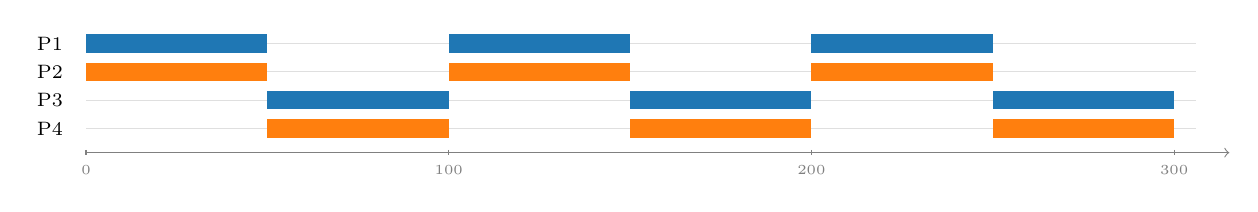
\begin{tikzpicture}[x=0.04606cm,y=0.36cm]
\node[anchor=east,font=\scriptsize] at (-3.7,3) {P1};
\draw[gray!25] (0,3) -- (306,3);
\node[anchor=east,font=\scriptsize] at (-3.7,2) {P2};
\draw[gray!25] (0,2) -- (306,2);
\node[anchor=east,font=\scriptsize] at (-3.7,1) {P3};
\draw[gray!25] (0,1) -- (306,1);
\node[anchor=east,font=\scriptsize] at (-3.7,0) {P4};
\draw[gray!25] (0,0) -- (306,0);
\fill[cCPU0] (0,2.68) rectangle (50,3.32);
\fill[cCPU0] (50,0.68) rectangle (100,1.32);
\fill[cCPU0] (100,2.68) rectangle (150,3.32);
\fill[cCPU0] (150,0.68) rectangle (200,1.32);
\fill[cCPU0] (200,2.68) rectangle (250,3.32);
\fill[cCPU0] (250,0.68) rectangle (300,1.32);
\fill[cCPU1] (0,1.68) rectangle (50,2.32);
\fill[cCPU1] (50,-0.32) rectangle (100,0.32);
\fill[cCPU1] (100,1.68) rectangle (150,2.32);
\fill[cCPU1] (150,-0.32) rectangle (200,0.32);
\fill[cCPU1] (200,1.68) rectangle (250,2.32);
\fill[cCPU1] (250,-0.32) rectangle (300,0.32);
\draw[->,gray] (0,-0.85) -- (315.2,-0.85);
\draw[gray] (0,-0.75)--(0,-0.95) node[below,font=\tiny]{0};
\draw[gray] (100,-0.75)--(100,-0.95) node[below,font=\tiny]{100};
\draw[gray] (200,-0.75)--(200,-0.95) node[below,font=\tiny]{200};
\draw[gray] (300,-0.75)--(300,-0.95) node[below,font=\tiny]{300};
\end{tikzpicture}\par
\par\vspace{1.5mm}{\small\textbf{RR}\quad(makespan 306, idle 12, 0 bursts migrated)}\par\vspace{0.8mm}
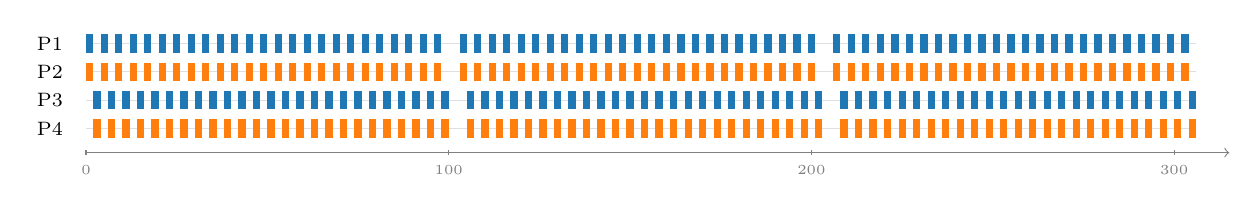
\begin{tikzpicture}[x=0.04606cm,y=0.36cm]
\node[anchor=east,font=\scriptsize] at (-3.7,3) {P1};
\draw[gray!25] (0,3) -- (306,3);
\node[anchor=east,font=\scriptsize] at (-3.7,2) {P2};
\draw[gray!25] (0,2) -- (306,2);
\node[anchor=east,font=\scriptsize] at (-3.7,1) {P3};
\draw[gray!25] (0,1) -- (306,1);
\node[anchor=east,font=\scriptsize] at (-3.7,0) {P4};
\draw[gray!25] (0,0) -- (306,0);
\fill[cCPU0] (0,2.68) rectangle (2,3.32);
\fill[cCPU0] (2,0.68) rectangle (4,1.32);
\fill[cCPU0] (4,2.68) rectangle (6,3.32);
\fill[cCPU0] (6,0.68) rectangle (8,1.32);
\fill[cCPU0] (8,2.68) rectangle (10,3.32);
\fill[cCPU0] (10,0.68) rectangle (12,1.32);
\fill[cCPU0] (12,2.68) rectangle (14,3.32);
\fill[cCPU0] (14,0.68) rectangle (16,1.32);
\fill[cCPU0] (16,2.68) rectangle (18,3.32);
\fill[cCPU0] (18,0.68) rectangle (20,1.32);
\fill[cCPU0] (20,2.68) rectangle (22,3.32);
\fill[cCPU0] (22,0.68) rectangle (24,1.32);
\fill[cCPU0] (24,2.68) rectangle (26,3.32);
\fill[cCPU0] (26,0.68) rectangle (28,1.32);
\fill[cCPU0] (28,2.68) rectangle (30,3.32);
\fill[cCPU0] (30,0.68) rectangle (32,1.32);
\fill[cCPU0] (32,2.68) rectangle (34,3.32);
\fill[cCPU0] (34,0.68) rectangle (36,1.32);
\fill[cCPU0] (36,2.68) rectangle (38,3.32);
\fill[cCPU0] (38,0.68) rectangle (40,1.32);
\fill[cCPU0] (40,2.68) rectangle (42,3.32);
\fill[cCPU0] (42,0.68) rectangle (44,1.32);
\fill[cCPU0] (44,2.68) rectangle (46,3.32);
\fill[cCPU0] (46,0.68) rectangle (48,1.32);
\fill[cCPU0] (48,2.68) rectangle (50,3.32);
\fill[cCPU0] (50,0.68) rectangle (52,1.32);
\fill[cCPU0] (52,2.68) rectangle (54,3.32);
\fill[cCPU0] (54,0.68) rectangle (56,1.32);
\fill[cCPU0] (56,2.68) rectangle (58,3.32);
\fill[cCPU0] (58,0.68) rectangle (60,1.32);
\fill[cCPU0] (60,2.68) rectangle (62,3.32);
\fill[cCPU0] (62,0.68) rectangle (64,1.32);
\fill[cCPU0] (64,2.68) rectangle (66,3.32);
\fill[cCPU0] (66,0.68) rectangle (68,1.32);
\fill[cCPU0] (68,2.68) rectangle (70,3.32);
\fill[cCPU0] (70,0.68) rectangle (72,1.32);
\fill[cCPU0] (72,2.68) rectangle (74,3.32);
\fill[cCPU0] (74,0.68) rectangle (76,1.32);
\fill[cCPU0] (76,2.68) rectangle (78,3.32);
\fill[cCPU0] (78,0.68) rectangle (80,1.32);
\fill[cCPU0] (80,2.68) rectangle (82,3.32);
\fill[cCPU0] (82,0.68) rectangle (84,1.32);
\fill[cCPU0] (84,2.68) rectangle (86,3.32);
\fill[cCPU0] (86,0.68) rectangle (88,1.32);
\fill[cCPU0] (88,2.68) rectangle (90,3.32);
\fill[cCPU0] (90,0.68) rectangle (92,1.32);
\fill[cCPU0] (92,2.68) rectangle (94,3.32);
\fill[cCPU0] (94,0.68) rectangle (96,1.32);
\fill[cCPU0] (96,2.68) rectangle (98,3.32);
\fill[cCPU0] (98,0.68) rectangle (100,1.32);
\fill[cCPU0] (103,2.68) rectangle (105,3.32);
\fill[cCPU0] (105,0.68) rectangle (107,1.32);
\fill[cCPU0] (107,2.68) rectangle (109,3.32);
\fill[cCPU0] (109,0.68) rectangle (111,1.32);
\fill[cCPU0] (111,2.68) rectangle (113,3.32);
\fill[cCPU0] (113,0.68) rectangle (115,1.32);
\fill[cCPU0] (115,2.68) rectangle (117,3.32);
\fill[cCPU0] (117,0.68) rectangle (119,1.32);
\fill[cCPU0] (119,2.68) rectangle (121,3.32);
\fill[cCPU0] (121,0.68) rectangle (123,1.32);
\fill[cCPU0] (123,2.68) rectangle (125,3.32);
\fill[cCPU0] (125,0.68) rectangle (127,1.32);
\fill[cCPU0] (127,2.68) rectangle (129,3.32);
\fill[cCPU0] (129,0.68) rectangle (131,1.32);
\fill[cCPU0] (131,2.68) rectangle (133,3.32);
\fill[cCPU0] (133,0.68) rectangle (135,1.32);
\fill[cCPU0] (135,2.68) rectangle (137,3.32);
\fill[cCPU0] (137,0.68) rectangle (139,1.32);
\fill[cCPU0] (139,2.68) rectangle (141,3.32);
\fill[cCPU0] (141,0.68) rectangle (143,1.32);
\fill[cCPU0] (143,2.68) rectangle (145,3.32);
\fill[cCPU0] (145,0.68) rectangle (147,1.32);
\fill[cCPU0] (147,2.68) rectangle (149,3.32);
\fill[cCPU0] (149,0.68) rectangle (151,1.32);
\fill[cCPU0] (151,2.68) rectangle (153,3.32);
\fill[cCPU0] (153,0.68) rectangle (155,1.32);
\fill[cCPU0] (155,2.68) rectangle (157,3.32);
\fill[cCPU0] (157,0.68) rectangle (159,1.32);
\fill[cCPU0] (159,2.68) rectangle (161,3.32);
\fill[cCPU0] (161,0.68) rectangle (163,1.32);
\fill[cCPU0] (163,2.68) rectangle (165,3.32);
\fill[cCPU0] (165,0.68) rectangle (167,1.32);
\fill[cCPU0] (167,2.68) rectangle (169,3.32);
\fill[cCPU0] (169,0.68) rectangle (171,1.32);
\fill[cCPU0] (171,2.68) rectangle (173,3.32);
\fill[cCPU0] (173,0.68) rectangle (175,1.32);
\fill[cCPU0] (175,2.68) rectangle (177,3.32);
\fill[cCPU0] (177,0.68) rectangle (179,1.32);
\fill[cCPU0] (179,2.68) rectangle (181,3.32);
\fill[cCPU0] (181,0.68) rectangle (183,1.32);
\fill[cCPU0] (183,2.68) rectangle (185,3.32);
\fill[cCPU0] (185,0.68) rectangle (187,1.32);
\fill[cCPU0] (187,2.68) rectangle (189,3.32);
\fill[cCPU0] (189,0.68) rectangle (191,1.32);
\fill[cCPU0] (191,2.68) rectangle (193,3.32);
\fill[cCPU0] (193,0.68) rectangle (195,1.32);
\fill[cCPU0] (195,2.68) rectangle (197,3.32);
\fill[cCPU0] (197,0.68) rectangle (199,1.32);
\fill[cCPU0] (199,2.68) rectangle (201,3.32);
\fill[cCPU0] (201,0.68) rectangle (203,1.32);
\fill[cCPU0] (206,2.68) rectangle (208,3.32);
\fill[cCPU0] (208,0.68) rectangle (210,1.32);
\fill[cCPU0] (210,2.68) rectangle (212,3.32);
\fill[cCPU0] (212,0.68) rectangle (214,1.32);
\fill[cCPU0] (214,2.68) rectangle (216,3.32);
\fill[cCPU0] (216,0.68) rectangle (218,1.32);
\fill[cCPU0] (218,2.68) rectangle (220,3.32);
\fill[cCPU0] (220,0.68) rectangle (222,1.32);
\fill[cCPU0] (222,2.68) rectangle (224,3.32);
\fill[cCPU0] (224,0.68) rectangle (226,1.32);
\fill[cCPU0] (226,2.68) rectangle (228,3.32);
\fill[cCPU0] (228,0.68) rectangle (230,1.32);
\fill[cCPU0] (230,2.68) rectangle (232,3.32);
\fill[cCPU0] (232,0.68) rectangle (234,1.32);
\fill[cCPU0] (234,2.68) rectangle (236,3.32);
\fill[cCPU0] (236,0.68) rectangle (238,1.32);
\fill[cCPU0] (238,2.68) rectangle (240,3.32);
\fill[cCPU0] (240,0.68) rectangle (242,1.32);
\fill[cCPU0] (242,2.68) rectangle (244,3.32);
\fill[cCPU0] (244,0.68) rectangle (246,1.32);
\fill[cCPU0] (246,2.68) rectangle (248,3.32);
\fill[cCPU0] (248,0.68) rectangle (250,1.32);
\fill[cCPU0] (250,2.68) rectangle (252,3.32);
\fill[cCPU0] (252,0.68) rectangle (254,1.32);
\fill[cCPU0] (254,2.68) rectangle (256,3.32);
\fill[cCPU0] (256,0.68) rectangle (258,1.32);
\fill[cCPU0] (258,2.68) rectangle (260,3.32);
\fill[cCPU0] (260,0.68) rectangle (262,1.32);
\fill[cCPU0] (262,2.68) rectangle (264,3.32);
\fill[cCPU0] (264,0.68) rectangle (266,1.32);
\fill[cCPU0] (266,2.68) rectangle (268,3.32);
\fill[cCPU0] (268,0.68) rectangle (270,1.32);
\fill[cCPU0] (270,2.68) rectangle (272,3.32);
\fill[cCPU0] (272,0.68) rectangle (274,1.32);
\fill[cCPU0] (274,2.68) rectangle (276,3.32);
\fill[cCPU0] (276,0.68) rectangle (278,1.32);
\fill[cCPU0] (278,2.68) rectangle (280,3.32);
\fill[cCPU0] (280,0.68) rectangle (282,1.32);
\fill[cCPU0] (282,2.68) rectangle (284,3.32);
\fill[cCPU0] (284,0.68) rectangle (286,1.32);
\fill[cCPU0] (286,2.68) rectangle (288,3.32);
\fill[cCPU0] (288,0.68) rectangle (290,1.32);
\fill[cCPU0] (290,2.68) rectangle (292,3.32);
\fill[cCPU0] (292,0.68) rectangle (294,1.32);
\fill[cCPU0] (294,2.68) rectangle (296,3.32);
\fill[cCPU0] (296,0.68) rectangle (298,1.32);
\fill[cCPU0] (298,2.68) rectangle (300,3.32);
\fill[cCPU0] (300,0.68) rectangle (302,1.32);
\fill[cCPU0] (302,2.68) rectangle (304,3.32);
\fill[cCPU0] (304,0.68) rectangle (306,1.32);
\fill[cCPU1] (0,1.68) rectangle (2,2.32);
\fill[cCPU1] (2,-0.32) rectangle (4,0.32);
\fill[cCPU1] (4,1.68) rectangle (6,2.32);
\fill[cCPU1] (6,-0.32) rectangle (8,0.32);
\fill[cCPU1] (8,1.68) rectangle (10,2.32);
\fill[cCPU1] (10,-0.32) rectangle (12,0.32);
\fill[cCPU1] (12,1.68) rectangle (14,2.32);
\fill[cCPU1] (14,-0.32) rectangle (16,0.32);
\fill[cCPU1] (16,1.68) rectangle (18,2.32);
\fill[cCPU1] (18,-0.32) rectangle (20,0.32);
\fill[cCPU1] (20,1.68) rectangle (22,2.32);
\fill[cCPU1] (22,-0.32) rectangle (24,0.32);
\fill[cCPU1] (24,1.68) rectangle (26,2.32);
\fill[cCPU1] (26,-0.32) rectangle (28,0.32);
\fill[cCPU1] (28,1.68) rectangle (30,2.32);
\fill[cCPU1] (30,-0.32) rectangle (32,0.32);
\fill[cCPU1] (32,1.68) rectangle (34,2.32);
\fill[cCPU1] (34,-0.32) rectangle (36,0.32);
\fill[cCPU1] (36,1.68) rectangle (38,2.32);
\fill[cCPU1] (38,-0.32) rectangle (40,0.32);
\fill[cCPU1] (40,1.68) rectangle (42,2.32);
\fill[cCPU1] (42,-0.32) rectangle (44,0.32);
\fill[cCPU1] (44,1.68) rectangle (46,2.32);
\fill[cCPU1] (46,-0.32) rectangle (48,0.32);
\fill[cCPU1] (48,1.68) rectangle (50,2.32);
\fill[cCPU1] (50,-0.32) rectangle (52,0.32);
\fill[cCPU1] (52,1.68) rectangle (54,2.32);
\fill[cCPU1] (54,-0.32) rectangle (56,0.32);
\fill[cCPU1] (56,1.68) rectangle (58,2.32);
\fill[cCPU1] (58,-0.32) rectangle (60,0.32);
\fill[cCPU1] (60,1.68) rectangle (62,2.32);
\fill[cCPU1] (62,-0.32) rectangle (64,0.32);
\fill[cCPU1] (64,1.68) rectangle (66,2.32);
\fill[cCPU1] (66,-0.32) rectangle (68,0.32);
\fill[cCPU1] (68,1.68) rectangle (70,2.32);
\fill[cCPU1] (70,-0.32) rectangle (72,0.32);
\fill[cCPU1] (72,1.68) rectangle (74,2.32);
\fill[cCPU1] (74,-0.32) rectangle (76,0.32);
\fill[cCPU1] (76,1.68) rectangle (78,2.32);
\fill[cCPU1] (78,-0.32) rectangle (80,0.32);
\fill[cCPU1] (80,1.68) rectangle (82,2.32);
\fill[cCPU1] (82,-0.32) rectangle (84,0.32);
\fill[cCPU1] (84,1.68) rectangle (86,2.32);
\fill[cCPU1] (86,-0.32) rectangle (88,0.32);
\fill[cCPU1] (88,1.68) rectangle (90,2.32);
\fill[cCPU1] (90,-0.32) rectangle (92,0.32);
\fill[cCPU1] (92,1.68) rectangle (94,2.32);
\fill[cCPU1] (94,-0.32) rectangle (96,0.32);
\fill[cCPU1] (96,1.68) rectangle (98,2.32);
\fill[cCPU1] (98,-0.32) rectangle (100,0.32);
\fill[cCPU1] (103,1.68) rectangle (105,2.32);
\fill[cCPU1] (105,-0.32) rectangle (107,0.32);
\fill[cCPU1] (107,1.68) rectangle (109,2.32);
\fill[cCPU1] (109,-0.32) rectangle (111,0.32);
\fill[cCPU1] (111,1.68) rectangle (113,2.32);
\fill[cCPU1] (113,-0.32) rectangle (115,0.32);
\fill[cCPU1] (115,1.68) rectangle (117,2.32);
\fill[cCPU1] (117,-0.32) rectangle (119,0.32);
\fill[cCPU1] (119,1.68) rectangle (121,2.32);
\fill[cCPU1] (121,-0.32) rectangle (123,0.32);
\fill[cCPU1] (123,1.68) rectangle (125,2.32);
\fill[cCPU1] (125,-0.32) rectangle (127,0.32);
\fill[cCPU1] (127,1.68) rectangle (129,2.32);
\fill[cCPU1] (129,-0.32) rectangle (131,0.32);
\fill[cCPU1] (131,1.68) rectangle (133,2.32);
\fill[cCPU1] (133,-0.32) rectangle (135,0.32);
\fill[cCPU1] (135,1.68) rectangle (137,2.32);
\fill[cCPU1] (137,-0.32) rectangle (139,0.32);
\fill[cCPU1] (139,1.68) rectangle (141,2.32);
\fill[cCPU1] (141,-0.32) rectangle (143,0.32);
\fill[cCPU1] (143,1.68) rectangle (145,2.32);
\fill[cCPU1] (145,-0.32) rectangle (147,0.32);
\fill[cCPU1] (147,1.68) rectangle (149,2.32);
\fill[cCPU1] (149,-0.32) rectangle (151,0.32);
\fill[cCPU1] (151,1.68) rectangle (153,2.32);
\fill[cCPU1] (153,-0.32) rectangle (155,0.32);
\fill[cCPU1] (155,1.68) rectangle (157,2.32);
\fill[cCPU1] (157,-0.32) rectangle (159,0.32);
\fill[cCPU1] (159,1.68) rectangle (161,2.32);
\fill[cCPU1] (161,-0.32) rectangle (163,0.32);
\fill[cCPU1] (163,1.68) rectangle (165,2.32);
\fill[cCPU1] (165,-0.32) rectangle (167,0.32);
\fill[cCPU1] (167,1.68) rectangle (169,2.32);
\fill[cCPU1] (169,-0.32) rectangle (171,0.32);
\fill[cCPU1] (171,1.68) rectangle (173,2.32);
\fill[cCPU1] (173,-0.32) rectangle (175,0.32);
\fill[cCPU1] (175,1.68) rectangle (177,2.32);
\fill[cCPU1] (177,-0.32) rectangle (179,0.32);
\fill[cCPU1] (179,1.68) rectangle (181,2.32);
\fill[cCPU1] (181,-0.32) rectangle (183,0.32);
\fill[cCPU1] (183,1.68) rectangle (185,2.32);
\fill[cCPU1] (185,-0.32) rectangle (187,0.32);
\fill[cCPU1] (187,1.68) rectangle (189,2.32);
\fill[cCPU1] (189,-0.32) rectangle (191,0.32);
\fill[cCPU1] (191,1.68) rectangle (193,2.32);
\fill[cCPU1] (193,-0.32) rectangle (195,0.32);
\fill[cCPU1] (195,1.68) rectangle (197,2.32);
\fill[cCPU1] (197,-0.32) rectangle (199,0.32);
\fill[cCPU1] (199,1.68) rectangle (201,2.32);
\fill[cCPU1] (201,-0.32) rectangle (203,0.32);
\fill[cCPU1] (206,1.68) rectangle (208,2.32);
\fill[cCPU1] (208,-0.32) rectangle (210,0.32);
\fill[cCPU1] (210,1.68) rectangle (212,2.32);
\fill[cCPU1] (212,-0.32) rectangle (214,0.32);
\fill[cCPU1] (214,1.68) rectangle (216,2.32);
\fill[cCPU1] (216,-0.32) rectangle (218,0.32);
\fill[cCPU1] (218,1.68) rectangle (220,2.32);
\fill[cCPU1] (220,-0.32) rectangle (222,0.32);
\fill[cCPU1] (222,1.68) rectangle (224,2.32);
\fill[cCPU1] (224,-0.32) rectangle (226,0.32);
\fill[cCPU1] (226,1.68) rectangle (228,2.32);
\fill[cCPU1] (228,-0.32) rectangle (230,0.32);
\fill[cCPU1] (230,1.68) rectangle (232,2.32);
\fill[cCPU1] (232,-0.32) rectangle (234,0.32);
\fill[cCPU1] (234,1.68) rectangle (236,2.32);
\fill[cCPU1] (236,-0.32) rectangle (238,0.32);
\fill[cCPU1] (238,1.68) rectangle (240,2.32);
\fill[cCPU1] (240,-0.32) rectangle (242,0.32);
\fill[cCPU1] (242,1.68) rectangle (244,2.32);
\fill[cCPU1] (244,-0.32) rectangle (246,0.32);
\fill[cCPU1] (246,1.68) rectangle (248,2.32);
\fill[cCPU1] (248,-0.32) rectangle (250,0.32);
\fill[cCPU1] (250,1.68) rectangle (252,2.32);
\fill[cCPU1] (252,-0.32) rectangle (254,0.32);
\fill[cCPU1] (254,1.68) rectangle (256,2.32);
\fill[cCPU1] (256,-0.32) rectangle (258,0.32);
\fill[cCPU1] (258,1.68) rectangle (260,2.32);
\fill[cCPU1] (260,-0.32) rectangle (262,0.32);
\fill[cCPU1] (262,1.68) rectangle (264,2.32);
\fill[cCPU1] (264,-0.32) rectangle (266,0.32);
\fill[cCPU1] (266,1.68) rectangle (268,2.32);
\fill[cCPU1] (268,-0.32) rectangle (270,0.32);
\fill[cCPU1] (270,1.68) rectangle (272,2.32);
\fill[cCPU1] (272,-0.32) rectangle (274,0.32);
\fill[cCPU1] (274,1.68) rectangle (276,2.32);
\fill[cCPU1] (276,-0.32) rectangle (278,0.32);
\fill[cCPU1] (278,1.68) rectangle (280,2.32);
\fill[cCPU1] (280,-0.32) rectangle (282,0.32);
\fill[cCPU1] (282,1.68) rectangle (284,2.32);
\fill[cCPU1] (284,-0.32) rectangle (286,0.32);
\fill[cCPU1] (286,1.68) rectangle (288,2.32);
\fill[cCPU1] (288,-0.32) rectangle (290,0.32);
\fill[cCPU1] (290,1.68) rectangle (292,2.32);
\fill[cCPU1] (292,-0.32) rectangle (294,0.32);
\fill[cCPU1] (294,1.68) rectangle (296,2.32);
\fill[cCPU1] (296,-0.32) rectangle (298,0.32);
\fill[cCPU1] (298,1.68) rectangle (300,2.32);
\fill[cCPU1] (300,-0.32) rectangle (302,0.32);
\fill[cCPU1] (302,1.68) rectangle (304,2.32);
\fill[cCPU1] (304,-0.32) rectangle (306,0.32);
\draw[->,gray] (0,-0.85) -- (315.2,-0.85);
\draw[gray] (0,-0.75)--(0,-0.95) node[below,font=\tiny]{0};
\draw[gray] (100,-0.75)--(100,-0.95) node[below,font=\tiny]{100};
\draw[gray] (200,-0.75)--(200,-0.95) node[below,font=\tiny]{200};
\draw[gray] (300,-0.75)--(300,-0.95) node[below,font=\tiny]{300};
\end{tikzpicture}\par
\par\vspace{1.5mm}{\small\textbf{MLFQ-NB}\quad(makespan 306, idle 12, 0 bursts migrated)}\par\vspace{0.8mm}
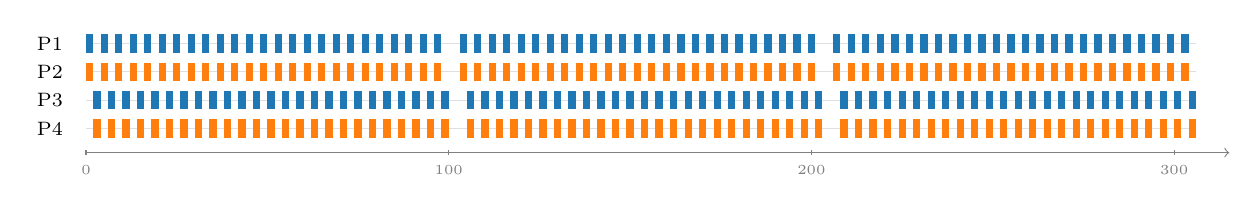
\begin{tikzpicture}[x=0.04606cm,y=0.36cm]
\node[anchor=east,font=\scriptsize] at (-3.7,3) {P1};
\draw[gray!25] (0,3) -- (306,3);
\node[anchor=east,font=\scriptsize] at (-3.7,2) {P2};
\draw[gray!25] (0,2) -- (306,2);
\node[anchor=east,font=\scriptsize] at (-3.7,1) {P3};
\draw[gray!25] (0,1) -- (306,1);
\node[anchor=east,font=\scriptsize] at (-3.7,0) {P4};
\draw[gray!25] (0,0) -- (306,0);
\fill[cCPU0] (0,2.68) rectangle (2,3.32);
\fill[cCPU0] (2,0.68) rectangle (4,1.32);
\fill[cCPU0] (4,2.68) rectangle (6,3.32);
\fill[cCPU0] (6,0.68) rectangle (8,1.32);
\fill[cCPU0] (8,2.68) rectangle (10,3.32);
\fill[cCPU0] (10,0.68) rectangle (12,1.32);
\fill[cCPU0] (12,2.68) rectangle (14,3.32);
\fill[cCPU0] (14,0.68) rectangle (16,1.32);
\fill[cCPU0] (16,2.68) rectangle (18,3.32);
\fill[cCPU0] (18,0.68) rectangle (20,1.32);
\fill[cCPU0] (20,2.68) rectangle (22,3.32);
\fill[cCPU0] (22,0.68) rectangle (24,1.32);
\fill[cCPU0] (24,2.68) rectangle (26,3.32);
\fill[cCPU0] (26,0.68) rectangle (28,1.32);
\fill[cCPU0] (28,2.68) rectangle (30,3.32);
\fill[cCPU0] (30,0.68) rectangle (32,1.32);
\fill[cCPU0] (32,2.68) rectangle (34,3.32);
\fill[cCPU0] (34,0.68) rectangle (36,1.32);
\fill[cCPU0] (36,2.68) rectangle (38,3.32);
\fill[cCPU0] (38,0.68) rectangle (40,1.32);
\fill[cCPU0] (40,2.68) rectangle (42,3.32);
\fill[cCPU0] (42,0.68) rectangle (44,1.32);
\fill[cCPU0] (44,2.68) rectangle (46,3.32);
\fill[cCPU0] (46,0.68) rectangle (48,1.32);
\fill[cCPU0] (48,2.68) rectangle (50,3.32);
\fill[cCPU0] (50,0.68) rectangle (52,1.32);
\fill[cCPU0] (52,2.68) rectangle (54,3.32);
\fill[cCPU0] (54,0.68) rectangle (56,1.32);
\fill[cCPU0] (56,2.68) rectangle (58,3.32);
\fill[cCPU0] (58,0.68) rectangle (60,1.32);
\fill[cCPU0] (60,2.68) rectangle (62,3.32);
\fill[cCPU0] (62,0.68) rectangle (64,1.32);
\fill[cCPU0] (64,2.68) rectangle (66,3.32);
\fill[cCPU0] (66,0.68) rectangle (68,1.32);
\fill[cCPU0] (68,2.68) rectangle (70,3.32);
\fill[cCPU0] (70,0.68) rectangle (72,1.32);
\fill[cCPU0] (72,2.68) rectangle (74,3.32);
\fill[cCPU0] (74,0.68) rectangle (76,1.32);
\fill[cCPU0] (76,2.68) rectangle (78,3.32);
\fill[cCPU0] (78,0.68) rectangle (80,1.32);
\fill[cCPU0] (80,2.68) rectangle (82,3.32);
\fill[cCPU0] (82,0.68) rectangle (84,1.32);
\fill[cCPU0] (84,2.68) rectangle (86,3.32);
\fill[cCPU0] (86,0.68) rectangle (88,1.32);
\fill[cCPU0] (88,2.68) rectangle (90,3.32);
\fill[cCPU0] (90,0.68) rectangle (92,1.32);
\fill[cCPU0] (92,2.68) rectangle (94,3.32);
\fill[cCPU0] (94,0.68) rectangle (96,1.32);
\fill[cCPU0] (96,2.68) rectangle (98,3.32);
\fill[cCPU0] (98,0.68) rectangle (100,1.32);
\fill[cCPU0] (103,2.68) rectangle (105,3.32);
\fill[cCPU0] (105,0.68) rectangle (107,1.32);
\fill[cCPU0] (107,2.68) rectangle (109,3.32);
\fill[cCPU0] (109,0.68) rectangle (111,1.32);
\fill[cCPU0] (111,2.68) rectangle (113,3.32);
\fill[cCPU0] (113,0.68) rectangle (115,1.32);
\fill[cCPU0] (115,2.68) rectangle (117,3.32);
\fill[cCPU0] (117,0.68) rectangle (119,1.32);
\fill[cCPU0] (119,2.68) rectangle (121,3.32);
\fill[cCPU0] (121,0.68) rectangle (123,1.32);
\fill[cCPU0] (123,2.68) rectangle (125,3.32);
\fill[cCPU0] (125,0.68) rectangle (127,1.32);
\fill[cCPU0] (127,2.68) rectangle (129,3.32);
\fill[cCPU0] (129,0.68) rectangle (131,1.32);
\fill[cCPU0] (131,2.68) rectangle (133,3.32);
\fill[cCPU0] (133,0.68) rectangle (135,1.32);
\fill[cCPU0] (135,2.68) rectangle (137,3.32);
\fill[cCPU0] (137,0.68) rectangle (139,1.32);
\fill[cCPU0] (139,2.68) rectangle (141,3.32);
\fill[cCPU0] (141,0.68) rectangle (143,1.32);
\fill[cCPU0] (143,2.68) rectangle (145,3.32);
\fill[cCPU0] (145,0.68) rectangle (147,1.32);
\fill[cCPU0] (147,2.68) rectangle (149,3.32);
\fill[cCPU0] (149,0.68) rectangle (151,1.32);
\fill[cCPU0] (151,2.68) rectangle (153,3.32);
\fill[cCPU0] (153,0.68) rectangle (155,1.32);
\fill[cCPU0] (155,2.68) rectangle (157,3.32);
\fill[cCPU0] (157,0.68) rectangle (159,1.32);
\fill[cCPU0] (159,2.68) rectangle (161,3.32);
\fill[cCPU0] (161,0.68) rectangle (163,1.32);
\fill[cCPU0] (163,2.68) rectangle (165,3.32);
\fill[cCPU0] (165,0.68) rectangle (167,1.32);
\fill[cCPU0] (167,2.68) rectangle (169,3.32);
\fill[cCPU0] (169,0.68) rectangle (171,1.32);
\fill[cCPU0] (171,2.68) rectangle (173,3.32);
\fill[cCPU0] (173,0.68) rectangle (175,1.32);
\fill[cCPU0] (175,2.68) rectangle (177,3.32);
\fill[cCPU0] (177,0.68) rectangle (179,1.32);
\fill[cCPU0] (179,2.68) rectangle (181,3.32);
\fill[cCPU0] (181,0.68) rectangle (183,1.32);
\fill[cCPU0] (183,2.68) rectangle (185,3.32);
\fill[cCPU0] (185,0.68) rectangle (187,1.32);
\fill[cCPU0] (187,2.68) rectangle (189,3.32);
\fill[cCPU0] (189,0.68) rectangle (191,1.32);
\fill[cCPU0] (191,2.68) rectangle (193,3.32);
\fill[cCPU0] (193,0.68) rectangle (195,1.32);
\fill[cCPU0] (195,2.68) rectangle (197,3.32);
\fill[cCPU0] (197,0.68) rectangle (199,1.32);
\fill[cCPU0] (199,2.68) rectangle (201,3.32);
\fill[cCPU0] (201,0.68) rectangle (203,1.32);
\fill[cCPU0] (206,2.68) rectangle (208,3.32);
\fill[cCPU0] (208,0.68) rectangle (210,1.32);
\fill[cCPU0] (210,2.68) rectangle (212,3.32);
\fill[cCPU0] (212,0.68) rectangle (214,1.32);
\fill[cCPU0] (214,2.68) rectangle (216,3.32);
\fill[cCPU0] (216,0.68) rectangle (218,1.32);
\fill[cCPU0] (218,2.68) rectangle (220,3.32);
\fill[cCPU0] (220,0.68) rectangle (222,1.32);
\fill[cCPU0] (222,2.68) rectangle (224,3.32);
\fill[cCPU0] (224,0.68) rectangle (226,1.32);
\fill[cCPU0] (226,2.68) rectangle (228,3.32);
\fill[cCPU0] (228,0.68) rectangle (230,1.32);
\fill[cCPU0] (230,2.68) rectangle (232,3.32);
\fill[cCPU0] (232,0.68) rectangle (234,1.32);
\fill[cCPU0] (234,2.68) rectangle (236,3.32);
\fill[cCPU0] (236,0.68) rectangle (238,1.32);
\fill[cCPU0] (238,2.68) rectangle (240,3.32);
\fill[cCPU0] (240,0.68) rectangle (242,1.32);
\fill[cCPU0] (242,2.68) rectangle (244,3.32);
\fill[cCPU0] (244,0.68) rectangle (246,1.32);
\fill[cCPU0] (246,2.68) rectangle (248,3.32);
\fill[cCPU0] (248,0.68) rectangle (250,1.32);
\fill[cCPU0] (250,2.68) rectangle (252,3.32);
\fill[cCPU0] (252,0.68) rectangle (254,1.32);
\fill[cCPU0] (254,2.68) rectangle (256,3.32);
\fill[cCPU0] (256,0.68) rectangle (258,1.32);
\fill[cCPU0] (258,2.68) rectangle (260,3.32);
\fill[cCPU0] (260,0.68) rectangle (262,1.32);
\fill[cCPU0] (262,2.68) rectangle (264,3.32);
\fill[cCPU0] (264,0.68) rectangle (266,1.32);
\fill[cCPU0] (266,2.68) rectangle (268,3.32);
\fill[cCPU0] (268,0.68) rectangle (270,1.32);
\fill[cCPU0] (270,2.68) rectangle (272,3.32);
\fill[cCPU0] (272,0.68) rectangle (274,1.32);
\fill[cCPU0] (274,2.68) rectangle (276,3.32);
\fill[cCPU0] (276,0.68) rectangle (278,1.32);
\fill[cCPU0] (278,2.68) rectangle (280,3.32);
\fill[cCPU0] (280,0.68) rectangle (282,1.32);
\fill[cCPU0] (282,2.68) rectangle (284,3.32);
\fill[cCPU0] (284,0.68) rectangle (286,1.32);
\fill[cCPU0] (286,2.68) rectangle (288,3.32);
\fill[cCPU0] (288,0.68) rectangle (290,1.32);
\fill[cCPU0] (290,2.68) rectangle (292,3.32);
\fill[cCPU0] (292,0.68) rectangle (294,1.32);
\fill[cCPU0] (294,2.68) rectangle (296,3.32);
\fill[cCPU0] (296,0.68) rectangle (298,1.32);
\fill[cCPU0] (298,2.68) rectangle (300,3.32);
\fill[cCPU0] (300,0.68) rectangle (302,1.32);
\fill[cCPU0] (302,2.68) rectangle (304,3.32);
\fill[cCPU0] (304,0.68) rectangle (306,1.32);
\fill[cCPU1] (0,1.68) rectangle (2,2.32);
\fill[cCPU1] (2,-0.32) rectangle (4,0.32);
\fill[cCPU1] (4,1.68) rectangle (6,2.32);
\fill[cCPU1] (6,-0.32) rectangle (8,0.32);
\fill[cCPU1] (8,1.68) rectangle (10,2.32);
\fill[cCPU1] (10,-0.32) rectangle (12,0.32);
\fill[cCPU1] (12,1.68) rectangle (14,2.32);
\fill[cCPU1] (14,-0.32) rectangle (16,0.32);
\fill[cCPU1] (16,1.68) rectangle (18,2.32);
\fill[cCPU1] (18,-0.32) rectangle (20,0.32);
\fill[cCPU1] (20,1.68) rectangle (22,2.32);
\fill[cCPU1] (22,-0.32) rectangle (24,0.32);
\fill[cCPU1] (24,1.68) rectangle (26,2.32);
\fill[cCPU1] (26,-0.32) rectangle (28,0.32);
\fill[cCPU1] (28,1.68) rectangle (30,2.32);
\fill[cCPU1] (30,-0.32) rectangle (32,0.32);
\fill[cCPU1] (32,1.68) rectangle (34,2.32);
\fill[cCPU1] (34,-0.32) rectangle (36,0.32);
\fill[cCPU1] (36,1.68) rectangle (38,2.32);
\fill[cCPU1] (38,-0.32) rectangle (40,0.32);
\fill[cCPU1] (40,1.68) rectangle (42,2.32);
\fill[cCPU1] (42,-0.32) rectangle (44,0.32);
\fill[cCPU1] (44,1.68) rectangle (46,2.32);
\fill[cCPU1] (46,-0.32) rectangle (48,0.32);
\fill[cCPU1] (48,1.68) rectangle (50,2.32);
\fill[cCPU1] (50,-0.32) rectangle (52,0.32);
\fill[cCPU1] (52,1.68) rectangle (54,2.32);
\fill[cCPU1] (54,-0.32) rectangle (56,0.32);
\fill[cCPU1] (56,1.68) rectangle (58,2.32);
\fill[cCPU1] (58,-0.32) rectangle (60,0.32);
\fill[cCPU1] (60,1.68) rectangle (62,2.32);
\fill[cCPU1] (62,-0.32) rectangle (64,0.32);
\fill[cCPU1] (64,1.68) rectangle (66,2.32);
\fill[cCPU1] (66,-0.32) rectangle (68,0.32);
\fill[cCPU1] (68,1.68) rectangle (70,2.32);
\fill[cCPU1] (70,-0.32) rectangle (72,0.32);
\fill[cCPU1] (72,1.68) rectangle (74,2.32);
\fill[cCPU1] (74,-0.32) rectangle (76,0.32);
\fill[cCPU1] (76,1.68) rectangle (78,2.32);
\fill[cCPU1] (78,-0.32) rectangle (80,0.32);
\fill[cCPU1] (80,1.68) rectangle (82,2.32);
\fill[cCPU1] (82,-0.32) rectangle (84,0.32);
\fill[cCPU1] (84,1.68) rectangle (86,2.32);
\fill[cCPU1] (86,-0.32) rectangle (88,0.32);
\fill[cCPU1] (88,1.68) rectangle (90,2.32);
\fill[cCPU1] (90,-0.32) rectangle (92,0.32);
\fill[cCPU1] (92,1.68) rectangle (94,2.32);
\fill[cCPU1] (94,-0.32) rectangle (96,0.32);
\fill[cCPU1] (96,1.68) rectangle (98,2.32);
\fill[cCPU1] (98,-0.32) rectangle (100,0.32);
\fill[cCPU1] (103,1.68) rectangle (105,2.32);
\fill[cCPU1] (105,-0.32) rectangle (107,0.32);
\fill[cCPU1] (107,1.68) rectangle (109,2.32);
\fill[cCPU1] (109,-0.32) rectangle (111,0.32);
\fill[cCPU1] (111,1.68) rectangle (113,2.32);
\fill[cCPU1] (113,-0.32) rectangle (115,0.32);
\fill[cCPU1] (115,1.68) rectangle (117,2.32);
\fill[cCPU1] (117,-0.32) rectangle (119,0.32);
\fill[cCPU1] (119,1.68) rectangle (121,2.32);
\fill[cCPU1] (121,-0.32) rectangle (123,0.32);
\fill[cCPU1] (123,1.68) rectangle (125,2.32);
\fill[cCPU1] (125,-0.32) rectangle (127,0.32);
\fill[cCPU1] (127,1.68) rectangle (129,2.32);
\fill[cCPU1] (129,-0.32) rectangle (131,0.32);
\fill[cCPU1] (131,1.68) rectangle (133,2.32);
\fill[cCPU1] (133,-0.32) rectangle (135,0.32);
\fill[cCPU1] (135,1.68) rectangle (137,2.32);
\fill[cCPU1] (137,-0.32) rectangle (139,0.32);
\fill[cCPU1] (139,1.68) rectangle (141,2.32);
\fill[cCPU1] (141,-0.32) rectangle (143,0.32);
\fill[cCPU1] (143,1.68) rectangle (145,2.32);
\fill[cCPU1] (145,-0.32) rectangle (147,0.32);
\fill[cCPU1] (147,1.68) rectangle (149,2.32);
\fill[cCPU1] (149,-0.32) rectangle (151,0.32);
\fill[cCPU1] (151,1.68) rectangle (153,2.32);
\fill[cCPU1] (153,-0.32) rectangle (155,0.32);
\fill[cCPU1] (155,1.68) rectangle (157,2.32);
\fill[cCPU1] (157,-0.32) rectangle (159,0.32);
\fill[cCPU1] (159,1.68) rectangle (161,2.32);
\fill[cCPU1] (161,-0.32) rectangle (163,0.32);
\fill[cCPU1] (163,1.68) rectangle (165,2.32);
\fill[cCPU1] (165,-0.32) rectangle (167,0.32);
\fill[cCPU1] (167,1.68) rectangle (169,2.32);
\fill[cCPU1] (169,-0.32) rectangle (171,0.32);
\fill[cCPU1] (171,1.68) rectangle (173,2.32);
\fill[cCPU1] (173,-0.32) rectangle (175,0.32);
\fill[cCPU1] (175,1.68) rectangle (177,2.32);
\fill[cCPU1] (177,-0.32) rectangle (179,0.32);
\fill[cCPU1] (179,1.68) rectangle (181,2.32);
\fill[cCPU1] (181,-0.32) rectangle (183,0.32);
\fill[cCPU1] (183,1.68) rectangle (185,2.32);
\fill[cCPU1] (185,-0.32) rectangle (187,0.32);
\fill[cCPU1] (187,1.68) rectangle (189,2.32);
\fill[cCPU1] (189,-0.32) rectangle (191,0.32);
\fill[cCPU1] (191,1.68) rectangle (193,2.32);
\fill[cCPU1] (193,-0.32) rectangle (195,0.32);
\fill[cCPU1] (195,1.68) rectangle (197,2.32);
\fill[cCPU1] (197,-0.32) rectangle (199,0.32);
\fill[cCPU1] (199,1.68) rectangle (201,2.32);
\fill[cCPU1] (201,-0.32) rectangle (203,0.32);
\fill[cCPU1] (206,1.68) rectangle (208,2.32);
\fill[cCPU1] (208,-0.32) rectangle (210,0.32);
\fill[cCPU1] (210,1.68) rectangle (212,2.32);
\fill[cCPU1] (212,-0.32) rectangle (214,0.32);
\fill[cCPU1] (214,1.68) rectangle (216,2.32);
\fill[cCPU1] (216,-0.32) rectangle (218,0.32);
\fill[cCPU1] (218,1.68) rectangle (220,2.32);
\fill[cCPU1] (220,-0.32) rectangle (222,0.32);
\fill[cCPU1] (222,1.68) rectangle (224,2.32);
\fill[cCPU1] (224,-0.32) rectangle (226,0.32);
\fill[cCPU1] (226,1.68) rectangle (228,2.32);
\fill[cCPU1] (228,-0.32) rectangle (230,0.32);
\fill[cCPU1] (230,1.68) rectangle (232,2.32);
\fill[cCPU1] (232,-0.32) rectangle (234,0.32);
\fill[cCPU1] (234,1.68) rectangle (236,2.32);
\fill[cCPU1] (236,-0.32) rectangle (238,0.32);
\fill[cCPU1] (238,1.68) rectangle (240,2.32);
\fill[cCPU1] (240,-0.32) rectangle (242,0.32);
\fill[cCPU1] (242,1.68) rectangle (244,2.32);
\fill[cCPU1] (244,-0.32) rectangle (246,0.32);
\fill[cCPU1] (246,1.68) rectangle (248,2.32);
\fill[cCPU1] (248,-0.32) rectangle (250,0.32);
\fill[cCPU1] (250,1.68) rectangle (252,2.32);
\fill[cCPU1] (252,-0.32) rectangle (254,0.32);
\fill[cCPU1] (254,1.68) rectangle (256,2.32);
\fill[cCPU1] (256,-0.32) rectangle (258,0.32);
\fill[cCPU1] (258,1.68) rectangle (260,2.32);
\fill[cCPU1] (260,-0.32) rectangle (262,0.32);
\fill[cCPU1] (262,1.68) rectangle (264,2.32);
\fill[cCPU1] (264,-0.32) rectangle (266,0.32);
\fill[cCPU1] (266,1.68) rectangle (268,2.32);
\fill[cCPU1] (268,-0.32) rectangle (270,0.32);
\fill[cCPU1] (270,1.68) rectangle (272,2.32);
\fill[cCPU1] (272,-0.32) rectangle (274,0.32);
\fill[cCPU1] (274,1.68) rectangle (276,2.32);
\fill[cCPU1] (276,-0.32) rectangle (278,0.32);
\fill[cCPU1] (278,1.68) rectangle (280,2.32);
\fill[cCPU1] (280,-0.32) rectangle (282,0.32);
\fill[cCPU1] (282,1.68) rectangle (284,2.32);
\fill[cCPU1] (284,-0.32) rectangle (286,0.32);
\fill[cCPU1] (286,1.68) rectangle (288,2.32);
\fill[cCPU1] (288,-0.32) rectangle (290,0.32);
\fill[cCPU1] (290,1.68) rectangle (292,2.32);
\fill[cCPU1] (292,-0.32) rectangle (294,0.32);
\fill[cCPU1] (294,1.68) rectangle (296,2.32);
\fill[cCPU1] (296,-0.32) rectangle (298,0.32);
\fill[cCPU1] (298,1.68) rectangle (300,2.32);
\fill[cCPU1] (300,-0.32) rectangle (302,0.32);
\fill[cCPU1] (302,1.68) rectangle (304,2.32);
\fill[cCPU1] (304,-0.32) rectangle (306,0.32);
\draw[->,gray] (0,-0.85) -- (315.2,-0.85);
\draw[gray] (0,-0.75)--(0,-0.95) node[below,font=\tiny]{0};
\draw[gray] (100,-0.75)--(100,-0.95) node[below,font=\tiny]{100};
\draw[gray] (200,-0.75)--(200,-0.95) node[below,font=\tiny]{200};
\draw[gray] (300,-0.75)--(300,-0.95) node[below,font=\tiny]{300};
\end{tikzpicture}\par
\par\vspace{1.5mm}{\small\textbf{MLFQ-WB}\quad(makespan 306, idle 12, 0 bursts migrated)}\par\vspace{0.8mm}
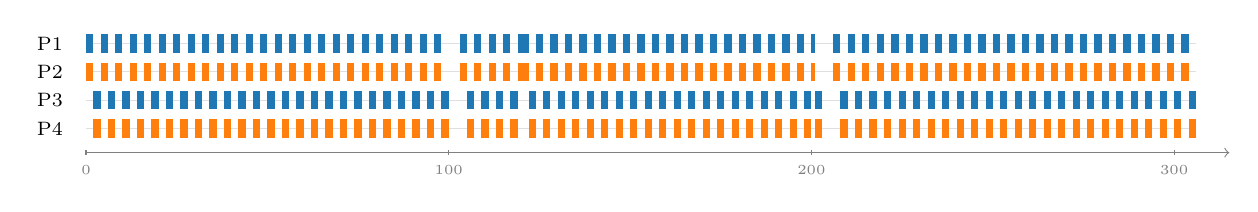
\begin{tikzpicture}[x=0.04606cm,y=0.36cm]
\node[anchor=east,font=\scriptsize] at (-3.7,3) {P1};
\draw[gray!25] (0,3) -- (306,3);
\node[anchor=east,font=\scriptsize] at (-3.7,2) {P2};
\draw[gray!25] (0,2) -- (306,2);
\node[anchor=east,font=\scriptsize] at (-3.7,1) {P3};
\draw[gray!25] (0,1) -- (306,1);
\node[anchor=east,font=\scriptsize] at (-3.7,0) {P4};
\draw[gray!25] (0,0) -- (306,0);
\fill[cCPU0] (0,2.68) rectangle (2,3.32);
\fill[cCPU0] (2,0.68) rectangle (4,1.32);
\fill[cCPU0] (4,2.68) rectangle (6,3.32);
\fill[cCPU0] (6,0.68) rectangle (8,1.32);
\fill[cCPU0] (8,2.68) rectangle (10,3.32);
\fill[cCPU0] (10,0.68) rectangle (12,1.32);
\fill[cCPU0] (12,2.68) rectangle (14,3.32);
\fill[cCPU0] (14,0.68) rectangle (16,1.32);
\fill[cCPU0] (16,2.68) rectangle (18,3.32);
\fill[cCPU0] (18,0.68) rectangle (20,1.32);
\fill[cCPU0] (20,2.68) rectangle (22,3.32);
\fill[cCPU0] (22,0.68) rectangle (24,1.32);
\fill[cCPU0] (24,2.68) rectangle (26,3.32);
\fill[cCPU0] (26,0.68) rectangle (28,1.32);
\fill[cCPU0] (28,2.68) rectangle (30,3.32);
\fill[cCPU0] (30,0.68) rectangle (32,1.32);
\fill[cCPU0] (32,2.68) rectangle (34,3.32);
\fill[cCPU0] (34,0.68) rectangle (36,1.32);
\fill[cCPU0] (36,2.68) rectangle (38,3.32);
\fill[cCPU0] (38,0.68) rectangle (40,1.32);
\fill[cCPU0] (40,2.68) rectangle (42,3.32);
\fill[cCPU0] (42,0.68) rectangle (44,1.32);
\fill[cCPU0] (44,2.68) rectangle (46,3.32);
\fill[cCPU0] (46,0.68) rectangle (48,1.32);
\fill[cCPU0] (48,2.68) rectangle (50,3.32);
\fill[cCPU0] (50,0.68) rectangle (52,1.32);
\fill[cCPU0] (52,2.68) rectangle (54,3.32);
\fill[cCPU0] (54,0.68) rectangle (56,1.32);
\fill[cCPU0] (56,2.68) rectangle (58,3.32);
\fill[cCPU0] (58,0.68) rectangle (60,1.32);
\fill[cCPU0] (60,2.68) rectangle (62,3.32);
\fill[cCPU0] (62,0.68) rectangle (64,1.32);
\fill[cCPU0] (64,2.68) rectangle (66,3.32);
\fill[cCPU0] (66,0.68) rectangle (68,1.32);
\fill[cCPU0] (68,2.68) rectangle (70,3.32);
\fill[cCPU0] (70,0.68) rectangle (72,1.32);
\fill[cCPU0] (72,2.68) rectangle (74,3.32);
\fill[cCPU0] (74,0.68) rectangle (76,1.32);
\fill[cCPU0] (76,2.68) rectangle (78,3.32);
\fill[cCPU0] (78,0.68) rectangle (80,1.32);
\fill[cCPU0] (80,2.68) rectangle (82,3.32);
\fill[cCPU0] (82,0.68) rectangle (84,1.32);
\fill[cCPU0] (84,2.68) rectangle (86,3.32);
\fill[cCPU0] (86,0.68) rectangle (88,1.32);
\fill[cCPU0] (88,2.68) rectangle (90,3.32);
\fill[cCPU0] (90,0.68) rectangle (92,1.32);
\fill[cCPU0] (92,2.68) rectangle (94,3.32);
\fill[cCPU0] (94,0.68) rectangle (96,1.32);
\fill[cCPU0] (96,2.68) rectangle (98,3.32);
\fill[cCPU0] (98,0.68) rectangle (100,1.32);
\fill[cCPU0] (103,2.68) rectangle (105,3.32);
\fill[cCPU0] (105,0.68) rectangle (107,1.32);
\fill[cCPU0] (107,2.68) rectangle (109,3.32);
\fill[cCPU0] (109,0.68) rectangle (111,1.32);
\fill[cCPU0] (111,2.68) rectangle (113,3.32);
\fill[cCPU0] (113,0.68) rectangle (115,1.32);
\fill[cCPU0] (115,2.68) rectangle (117,3.32);
\fill[cCPU0] (117,0.68) rectangle (119,1.32);
\fill[cCPU0] (119,2.68) rectangle (122,3.32);
\fill[cCPU0] (122,0.68) rectangle (124,1.32);
\fill[cCPU0] (124,2.68) rectangle (126,3.32);
\fill[cCPU0] (126,0.68) rectangle (128,1.32);
\fill[cCPU0] (128,2.68) rectangle (130,3.32);
\fill[cCPU0] (130,0.68) rectangle (132,1.32);
\fill[cCPU0] (132,2.68) rectangle (134,3.32);
\fill[cCPU0] (134,0.68) rectangle (136,1.32);
\fill[cCPU0] (136,2.68) rectangle (138,3.32);
\fill[cCPU0] (138,0.68) rectangle (140,1.32);
\fill[cCPU0] (140,2.68) rectangle (142,3.32);
\fill[cCPU0] (142,0.68) rectangle (144,1.32);
\fill[cCPU0] (144,2.68) rectangle (146,3.32);
\fill[cCPU0] (146,0.68) rectangle (148,1.32);
\fill[cCPU0] (148,2.68) rectangle (150,3.32);
\fill[cCPU0] (150,0.68) rectangle (152,1.32);
\fill[cCPU0] (152,2.68) rectangle (154,3.32);
\fill[cCPU0] (154,0.68) rectangle (156,1.32);
\fill[cCPU0] (156,2.68) rectangle (158,3.32);
\fill[cCPU0] (158,0.68) rectangle (160,1.32);
\fill[cCPU0] (160,2.68) rectangle (162,3.32);
\fill[cCPU0] (162,0.68) rectangle (164,1.32);
\fill[cCPU0] (164,2.68) rectangle (166,3.32);
\fill[cCPU0] (166,0.68) rectangle (168,1.32);
\fill[cCPU0] (168,2.68) rectangle (170,3.32);
\fill[cCPU0] (170,0.68) rectangle (172,1.32);
\fill[cCPU0] (172,2.68) rectangle (174,3.32);
\fill[cCPU0] (174,0.68) rectangle (176,1.32);
\fill[cCPU0] (176,2.68) rectangle (178,3.32);
\fill[cCPU0] (178,0.68) rectangle (180,1.32);
\fill[cCPU0] (180,2.68) rectangle (182,3.32);
\fill[cCPU0] (182,0.68) rectangle (184,1.32);
\fill[cCPU0] (184,2.68) rectangle (186,3.32);
\fill[cCPU0] (186,0.68) rectangle (188,1.32);
\fill[cCPU0] (188,2.68) rectangle (190,3.32);
\fill[cCPU0] (190,0.68) rectangle (192,1.32);
\fill[cCPU0] (192,2.68) rectangle (194,3.32);
\fill[cCPU0] (194,0.68) rectangle (196,1.32);
\fill[cCPU0] (196,2.68) rectangle (198,3.32);
\fill[cCPU0] (198,0.68) rectangle (200,1.32);
\fill[cCPU0] (200,2.68) rectangle (201,3.32);
\fill[cCPU0] (201,0.68) rectangle (203,1.32);
\fill[cCPU0] (206,2.68) rectangle (208,3.32);
\fill[cCPU0] (208,0.68) rectangle (210,1.32);
\fill[cCPU0] (210,2.68) rectangle (212,3.32);
\fill[cCPU0] (212,0.68) rectangle (214,1.32);
\fill[cCPU0] (214,2.68) rectangle (216,3.32);
\fill[cCPU0] (216,0.68) rectangle (218,1.32);
\fill[cCPU0] (218,2.68) rectangle (220,3.32);
\fill[cCPU0] (220,0.68) rectangle (222,1.32);
\fill[cCPU0] (222,2.68) rectangle (224,3.32);
\fill[cCPU0] (224,0.68) rectangle (226,1.32);
\fill[cCPU0] (226,2.68) rectangle (228,3.32);
\fill[cCPU0] (228,0.68) rectangle (230,1.32);
\fill[cCPU0] (230,2.68) rectangle (232,3.32);
\fill[cCPU0] (232,0.68) rectangle (234,1.32);
\fill[cCPU0] (234,2.68) rectangle (236,3.32);
\fill[cCPU0] (236,0.68) rectangle (238,1.32);
\fill[cCPU0] (238,2.68) rectangle (240,3.32);
\fill[cCPU0] (240,0.68) rectangle (242,1.32);
\fill[cCPU0] (242,2.68) rectangle (244,3.32);
\fill[cCPU0] (244,0.68) rectangle (246,1.32);
\fill[cCPU0] (246,2.68) rectangle (248,3.32);
\fill[cCPU0] (248,0.68) rectangle (250,1.32);
\fill[cCPU0] (250,2.68) rectangle (252,3.32);
\fill[cCPU0] (252,0.68) rectangle (254,1.32);
\fill[cCPU0] (254,2.68) rectangle (256,3.32);
\fill[cCPU0] (256,0.68) rectangle (258,1.32);
\fill[cCPU0] (258,2.68) rectangle (260,3.32);
\fill[cCPU0] (260,0.68) rectangle (262,1.32);
\fill[cCPU0] (262,2.68) rectangle (264,3.32);
\fill[cCPU0] (264,0.68) rectangle (266,1.32);
\fill[cCPU0] (266,2.68) rectangle (268,3.32);
\fill[cCPU0] (268,0.68) rectangle (270,1.32);
\fill[cCPU0] (270,2.68) rectangle (272,3.32);
\fill[cCPU0] (272,0.68) rectangle (274,1.32);
\fill[cCPU0] (274,2.68) rectangle (276,3.32);
\fill[cCPU0] (276,0.68) rectangle (278,1.32);
\fill[cCPU0] (278,2.68) rectangle (280,3.32);
\fill[cCPU0] (280,0.68) rectangle (282,1.32);
\fill[cCPU0] (282,2.68) rectangle (284,3.32);
\fill[cCPU0] (284,0.68) rectangle (286,1.32);
\fill[cCPU0] (286,2.68) rectangle (288,3.32);
\fill[cCPU0] (288,0.68) rectangle (290,1.32);
\fill[cCPU0] (290,2.68) rectangle (292,3.32);
\fill[cCPU0] (292,0.68) rectangle (294,1.32);
\fill[cCPU0] (294,2.68) rectangle (296,3.32);
\fill[cCPU0] (296,0.68) rectangle (298,1.32);
\fill[cCPU0] (298,2.68) rectangle (300,3.32);
\fill[cCPU0] (300,0.68) rectangle (302,1.32);
\fill[cCPU0] (302,2.68) rectangle (304,3.32);
\fill[cCPU0] (304,0.68) rectangle (306,1.32);
\fill[cCPU1] (0,1.68) rectangle (2,2.32);
\fill[cCPU1] (2,-0.32) rectangle (4,0.32);
\fill[cCPU1] (4,1.68) rectangle (6,2.32);
\fill[cCPU1] (6,-0.32) rectangle (8,0.32);
\fill[cCPU1] (8,1.68) rectangle (10,2.32);
\fill[cCPU1] (10,-0.32) rectangle (12,0.32);
\fill[cCPU1] (12,1.68) rectangle (14,2.32);
\fill[cCPU1] (14,-0.32) rectangle (16,0.32);
\fill[cCPU1] (16,1.68) rectangle (18,2.32);
\fill[cCPU1] (18,-0.32) rectangle (20,0.32);
\fill[cCPU1] (20,1.68) rectangle (22,2.32);
\fill[cCPU1] (22,-0.32) rectangle (24,0.32);
\fill[cCPU1] (24,1.68) rectangle (26,2.32);
\fill[cCPU1] (26,-0.32) rectangle (28,0.32);
\fill[cCPU1] (28,1.68) rectangle (30,2.32);
\fill[cCPU1] (30,-0.32) rectangle (32,0.32);
\fill[cCPU1] (32,1.68) rectangle (34,2.32);
\fill[cCPU1] (34,-0.32) rectangle (36,0.32);
\fill[cCPU1] (36,1.68) rectangle (38,2.32);
\fill[cCPU1] (38,-0.32) rectangle (40,0.32);
\fill[cCPU1] (40,1.68) rectangle (42,2.32);
\fill[cCPU1] (42,-0.32) rectangle (44,0.32);
\fill[cCPU1] (44,1.68) rectangle (46,2.32);
\fill[cCPU1] (46,-0.32) rectangle (48,0.32);
\fill[cCPU1] (48,1.68) rectangle (50,2.32);
\fill[cCPU1] (50,-0.32) rectangle (52,0.32);
\fill[cCPU1] (52,1.68) rectangle (54,2.32);
\fill[cCPU1] (54,-0.32) rectangle (56,0.32);
\fill[cCPU1] (56,1.68) rectangle (58,2.32);
\fill[cCPU1] (58,-0.32) rectangle (60,0.32);
\fill[cCPU1] (60,1.68) rectangle (62,2.32);
\fill[cCPU1] (62,-0.32) rectangle (64,0.32);
\fill[cCPU1] (64,1.68) rectangle (66,2.32);
\fill[cCPU1] (66,-0.32) rectangle (68,0.32);
\fill[cCPU1] (68,1.68) rectangle (70,2.32);
\fill[cCPU1] (70,-0.32) rectangle (72,0.32);
\fill[cCPU1] (72,1.68) rectangle (74,2.32);
\fill[cCPU1] (74,-0.32) rectangle (76,0.32);
\fill[cCPU1] (76,1.68) rectangle (78,2.32);
\fill[cCPU1] (78,-0.32) rectangle (80,0.32);
\fill[cCPU1] (80,1.68) rectangle (82,2.32);
\fill[cCPU1] (82,-0.32) rectangle (84,0.32);
\fill[cCPU1] (84,1.68) rectangle (86,2.32);
\fill[cCPU1] (86,-0.32) rectangle (88,0.32);
\fill[cCPU1] (88,1.68) rectangle (90,2.32);
\fill[cCPU1] (90,-0.32) rectangle (92,0.32);
\fill[cCPU1] (92,1.68) rectangle (94,2.32);
\fill[cCPU1] (94,-0.32) rectangle (96,0.32);
\fill[cCPU1] (96,1.68) rectangle (98,2.32);
\fill[cCPU1] (98,-0.32) rectangle (100,0.32);
\fill[cCPU1] (103,1.68) rectangle (105,2.32);
\fill[cCPU1] (105,-0.32) rectangle (107,0.32);
\fill[cCPU1] (107,1.68) rectangle (109,2.32);
\fill[cCPU1] (109,-0.32) rectangle (111,0.32);
\fill[cCPU1] (111,1.68) rectangle (113,2.32);
\fill[cCPU1] (113,-0.32) rectangle (115,0.32);
\fill[cCPU1] (115,1.68) rectangle (117,2.32);
\fill[cCPU1] (117,-0.32) rectangle (119,0.32);
\fill[cCPU1] (119,1.68) rectangle (122,2.32);
\fill[cCPU1] (122,-0.32) rectangle (124,0.32);
\fill[cCPU1] (124,1.68) rectangle (126,2.32);
\fill[cCPU1] (126,-0.32) rectangle (128,0.32);
\fill[cCPU1] (128,1.68) rectangle (130,2.32);
\fill[cCPU1] (130,-0.32) rectangle (132,0.32);
\fill[cCPU1] (132,1.68) rectangle (134,2.32);
\fill[cCPU1] (134,-0.32) rectangle (136,0.32);
\fill[cCPU1] (136,1.68) rectangle (138,2.32);
\fill[cCPU1] (138,-0.32) rectangle (140,0.32);
\fill[cCPU1] (140,1.68) rectangle (142,2.32);
\fill[cCPU1] (142,-0.32) rectangle (144,0.32);
\fill[cCPU1] (144,1.68) rectangle (146,2.32);
\fill[cCPU1] (146,-0.32) rectangle (148,0.32);
\fill[cCPU1] (148,1.68) rectangle (150,2.32);
\fill[cCPU1] (150,-0.32) rectangle (152,0.32);
\fill[cCPU1] (152,1.68) rectangle (154,2.32);
\fill[cCPU1] (154,-0.32) rectangle (156,0.32);
\fill[cCPU1] (156,1.68) rectangle (158,2.32);
\fill[cCPU1] (158,-0.32) rectangle (160,0.32);
\fill[cCPU1] (160,1.68) rectangle (162,2.32);
\fill[cCPU1] (162,-0.32) rectangle (164,0.32);
\fill[cCPU1] (164,1.68) rectangle (166,2.32);
\fill[cCPU1] (166,-0.32) rectangle (168,0.32);
\fill[cCPU1] (168,1.68) rectangle (170,2.32);
\fill[cCPU1] (170,-0.32) rectangle (172,0.32);
\fill[cCPU1] (172,1.68) rectangle (174,2.32);
\fill[cCPU1] (174,-0.32) rectangle (176,0.32);
\fill[cCPU1] (176,1.68) rectangle (178,2.32);
\fill[cCPU1] (178,-0.32) rectangle (180,0.32);
\fill[cCPU1] (180,1.68) rectangle (182,2.32);
\fill[cCPU1] (182,-0.32) rectangle (184,0.32);
\fill[cCPU1] (184,1.68) rectangle (186,2.32);
\fill[cCPU1] (186,-0.32) rectangle (188,0.32);
\fill[cCPU1] (188,1.68) rectangle (190,2.32);
\fill[cCPU1] (190,-0.32) rectangle (192,0.32);
\fill[cCPU1] (192,1.68) rectangle (194,2.32);
\fill[cCPU1] (194,-0.32) rectangle (196,0.32);
\fill[cCPU1] (196,1.68) rectangle (198,2.32);
\fill[cCPU1] (198,-0.32) rectangle (200,0.32);
\fill[cCPU1] (200,1.68) rectangle (201,2.32);
\fill[cCPU1] (201,-0.32) rectangle (203,0.32);
\fill[cCPU1] (206,1.68) rectangle (208,2.32);
\fill[cCPU1] (208,-0.32) rectangle (210,0.32);
\fill[cCPU1] (210,1.68) rectangle (212,2.32);
\fill[cCPU1] (212,-0.32) rectangle (214,0.32);
\fill[cCPU1] (214,1.68) rectangle (216,2.32);
\fill[cCPU1] (216,-0.32) rectangle (218,0.32);
\fill[cCPU1] (218,1.68) rectangle (220,2.32);
\fill[cCPU1] (220,-0.32) rectangle (222,0.32);
\fill[cCPU1] (222,1.68) rectangle (224,2.32);
\fill[cCPU1] (224,-0.32) rectangle (226,0.32);
\fill[cCPU1] (226,1.68) rectangle (228,2.32);
\fill[cCPU1] (228,-0.32) rectangle (230,0.32);
\fill[cCPU1] (230,1.68) rectangle (232,2.32);
\fill[cCPU1] (232,-0.32) rectangle (234,0.32);
\fill[cCPU1] (234,1.68) rectangle (236,2.32);
\fill[cCPU1] (236,-0.32) rectangle (238,0.32);
\fill[cCPU1] (238,1.68) rectangle (240,2.32);
\fill[cCPU1] (240,-0.32) rectangle (242,0.32);
\fill[cCPU1] (242,1.68) rectangle (244,2.32);
\fill[cCPU1] (244,-0.32) rectangle (246,0.32);
\fill[cCPU1] (246,1.68) rectangle (248,2.32);
\fill[cCPU1] (248,-0.32) rectangle (250,0.32);
\fill[cCPU1] (250,1.68) rectangle (252,2.32);
\fill[cCPU1] (252,-0.32) rectangle (254,0.32);
\fill[cCPU1] (254,1.68) rectangle (256,2.32);
\fill[cCPU1] (256,-0.32) rectangle (258,0.32);
\fill[cCPU1] (258,1.68) rectangle (260,2.32);
\fill[cCPU1] (260,-0.32) rectangle (262,0.32);
\fill[cCPU1] (262,1.68) rectangle (264,2.32);
\fill[cCPU1] (264,-0.32) rectangle (266,0.32);
\fill[cCPU1] (266,1.68) rectangle (268,2.32);
\fill[cCPU1] (268,-0.32) rectangle (270,0.32);
\fill[cCPU1] (270,1.68) rectangle (272,2.32);
\fill[cCPU1] (272,-0.32) rectangle (274,0.32);
\fill[cCPU1] (274,1.68) rectangle (276,2.32);
\fill[cCPU1] (276,-0.32) rectangle (278,0.32);
\fill[cCPU1] (278,1.68) rectangle (280,2.32);
\fill[cCPU1] (280,-0.32) rectangle (282,0.32);
\fill[cCPU1] (282,1.68) rectangle (284,2.32);
\fill[cCPU1] (284,-0.32) rectangle (286,0.32);
\fill[cCPU1] (286,1.68) rectangle (288,2.32);
\fill[cCPU1] (288,-0.32) rectangle (290,0.32);
\fill[cCPU1] (290,1.68) rectangle (292,2.32);
\fill[cCPU1] (292,-0.32) rectangle (294,0.32);
\fill[cCPU1] (294,1.68) rectangle (296,2.32);
\fill[cCPU1] (296,-0.32) rectangle (298,0.32);
\fill[cCPU1] (298,1.68) rectangle (300,2.32);
\fill[cCPU1] (300,-0.32) rectangle (302,0.32);
\fill[cCPU1] (302,1.68) rectangle (304,2.32);
\fill[cCPU1] (304,-0.32) rectangle (306,0.32);
\draw[->,gray] (0,-0.85) -- (315.2,-0.85);
\draw[gray] (0,-0.75)--(0,-0.95) node[below,font=\tiny]{0};
\draw[gray] (100,-0.75)--(100,-0.95) node[below,font=\tiny]{100};
\draw[gray] (200,-0.75)--(200,-0.95) node[below,font=\tiny]{200};
\draw[gray] (300,-0.75)--(300,-0.95) node[below,font=\tiny]{300};
\end{tikzpicture}\par
\caption{Workload 2, dual processor. The four identical processes pair up on the two processors. Under every policy each process stays on a single processor for its entire lifetime (P1 and P3 on CPU0; P2 and P4 on CPU1), because the processes always re-enter the shared queue in the same order and are therefore repeatedly dispatched to the same processor.}
\label{fig:gantt-dual-2}
\end{figure}
\begin{figure}[H]\centering
{\small\tikz{\fill[cCPU0] (0,0) rectangle (0.35,0.22);}~CPU0\qquad\tikz{\fill[cCPU1] (0,0) rectangle (0.35,0.22);}~CPU1}\par
\par\vspace{1.5mm}{\small\textbf{FIFO}\quad(makespan 14, idle 16, 0 bursts migrated)}\par\vspace{0.8mm}
\begin{tikzpicture}[x=1.00680cm,y=0.36cm]
\node[anchor=east,font=\scriptsize] at (-0.2,3) {P1};
\draw[gray!25] (0,3) -- (14,3);
\node[anchor=east,font=\scriptsize] at (-0.2,2) {P2};
\draw[gray!25] (0,2) -- (14,2);
\node[anchor=east,font=\scriptsize] at (-0.2,1) {P3};
\draw[gray!25] (0,1) -- (14,1);
\node[anchor=east,font=\scriptsize] at (-0.2,0) {P4};
\draw[gray!25] (0,0) -- (14,0);
\fill[cCPU0] (0,2.68) rectangle (1,3.32);
\fill[cCPU0] (1,0.68) rectangle (2,1.32);
\fill[cCPU0] (6,2.68) rectangle (7,3.32);
\fill[cCPU0] (7,0.68) rectangle (8,1.32);
\fill[cCPU0] (12,2.68) rectangle (13,3.32);
\fill[cCPU0] (13,0.68) rectangle (14,1.32);
\fill[cCPU1] (0,1.68) rectangle (1,2.32);
\fill[cCPU1] (1,-0.32) rectangle (2,0.32);
\fill[cCPU1] (6,1.68) rectangle (7,2.32);
\fill[cCPU1] (7,-0.32) rectangle (8,0.32);
\fill[cCPU1] (12,1.68) rectangle (13,2.32);
\fill[cCPU1] (13,-0.32) rectangle (14,0.32);
\draw[->,gray] (0,-0.85) -- (14.4,-0.85);
\draw[gray] (0,-0.75)--(0,-0.95) node[below,font=\tiny]{0};
\draw[gray] (5,-0.75)--(5,-0.95) node[below,font=\tiny]{5};
\draw[gray] (10,-0.75)--(10,-0.95) node[below,font=\tiny]{10};
\end{tikzpicture}\par
\par\vspace{1.5mm}{\small\textbf{RR}\quad(makespan 14, idle 16, 0 bursts migrated)}\par\vspace{0.8mm}
\begin{tikzpicture}[x=1.00680cm,y=0.36cm]
\node[anchor=east,font=\scriptsize] at (-0.2,3) {P1};
\draw[gray!25] (0,3) -- (14,3);
\node[anchor=east,font=\scriptsize] at (-0.2,2) {P2};
\draw[gray!25] (0,2) -- (14,2);
\node[anchor=east,font=\scriptsize] at (-0.2,1) {P3};
\draw[gray!25] (0,1) -- (14,1);
\node[anchor=east,font=\scriptsize] at (-0.2,0) {P4};
\draw[gray!25] (0,0) -- (14,0);
\fill[cCPU0] (0,2.68) rectangle (1,3.32);
\fill[cCPU0] (1,0.68) rectangle (2,1.32);
\fill[cCPU0] (6,2.68) rectangle (7,3.32);
\fill[cCPU0] (7,0.68) rectangle (8,1.32);
\fill[cCPU0] (12,2.68) rectangle (13,3.32);
\fill[cCPU0] (13,0.68) rectangle (14,1.32);
\fill[cCPU1] (0,1.68) rectangle (1,2.32);
\fill[cCPU1] (1,-0.32) rectangle (2,0.32);
\fill[cCPU1] (6,1.68) rectangle (7,2.32);
\fill[cCPU1] (7,-0.32) rectangle (8,0.32);
\fill[cCPU1] (12,1.68) rectangle (13,2.32);
\fill[cCPU1] (13,-0.32) rectangle (14,0.32);
\draw[->,gray] (0,-0.85) -- (14.4,-0.85);
\draw[gray] (0,-0.75)--(0,-0.95) node[below,font=\tiny]{0};
\draw[gray] (5,-0.75)--(5,-0.95) node[below,font=\tiny]{5};
\draw[gray] (10,-0.75)--(10,-0.95) node[below,font=\tiny]{10};
\end{tikzpicture}\par
\par\vspace{1.5mm}{\small\textbf{MLFQ-NB}\quad(makespan 14, idle 16, 0 bursts migrated)}\par\vspace{0.8mm}
\begin{tikzpicture}[x=1.00680cm,y=0.36cm]
\node[anchor=east,font=\scriptsize] at (-0.2,3) {P1};
\draw[gray!25] (0,3) -- (14,3);
\node[anchor=east,font=\scriptsize] at (-0.2,2) {P2};
\draw[gray!25] (0,2) -- (14,2);
\node[anchor=east,font=\scriptsize] at (-0.2,1) {P3};
\draw[gray!25] (0,1) -- (14,1);
\node[anchor=east,font=\scriptsize] at (-0.2,0) {P4};
\draw[gray!25] (0,0) -- (14,0);
\fill[cCPU0] (0,2.68) rectangle (1,3.32);
\fill[cCPU0] (1,0.68) rectangle (2,1.32);
\fill[cCPU0] (6,2.68) rectangle (7,3.32);
\fill[cCPU0] (7,0.68) rectangle (8,1.32);
\fill[cCPU0] (12,2.68) rectangle (13,3.32);
\fill[cCPU0] (13,0.68) rectangle (14,1.32);
\fill[cCPU1] (0,1.68) rectangle (1,2.32);
\fill[cCPU1] (1,-0.32) rectangle (2,0.32);
\fill[cCPU1] (6,1.68) rectangle (7,2.32);
\fill[cCPU1] (7,-0.32) rectangle (8,0.32);
\fill[cCPU1] (12,1.68) rectangle (13,2.32);
\fill[cCPU1] (13,-0.32) rectangle (14,0.32);
\draw[->,gray] (0,-0.85) -- (14.4,-0.85);
\draw[gray] (0,-0.75)--(0,-0.95) node[below,font=\tiny]{0};
\draw[gray] (5,-0.75)--(5,-0.95) node[below,font=\tiny]{5};
\draw[gray] (10,-0.75)--(10,-0.95) node[below,font=\tiny]{10};
\end{tikzpicture}\par
\par\vspace{1.5mm}{\small\textbf{MLFQ-WB}\quad(makespan 14, idle 16, 0 bursts migrated)}\par\vspace{0.8mm}
\begin{tikzpicture}[x=1.00680cm,y=0.36cm]
\node[anchor=east,font=\scriptsize] at (-0.2,3) {P1};
\draw[gray!25] (0,3) -- (14,3);
\node[anchor=east,font=\scriptsize] at (-0.2,2) {P2};
\draw[gray!25] (0,2) -- (14,2);
\node[anchor=east,font=\scriptsize] at (-0.2,1) {P3};
\draw[gray!25] (0,1) -- (14,1);
\node[anchor=east,font=\scriptsize] at (-0.2,0) {P4};
\draw[gray!25] (0,0) -- (14,0);
\fill[cCPU0] (0,2.68) rectangle (1,3.32);
\fill[cCPU0] (1,0.68) rectangle (2,1.32);
\fill[cCPU0] (6,2.68) rectangle (7,3.32);
\fill[cCPU0] (7,0.68) rectangle (8,1.32);
\fill[cCPU0] (12,2.68) rectangle (13,3.32);
\fill[cCPU0] (13,0.68) rectangle (14,1.32);
\fill[cCPU1] (0,1.68) rectangle (1,2.32);
\fill[cCPU1] (1,-0.32) rectangle (2,0.32);
\fill[cCPU1] (6,1.68) rectangle (7,2.32);
\fill[cCPU1] (7,-0.32) rectangle (8,0.32);
\fill[cCPU1] (12,1.68) rectangle (13,2.32);
\fill[cCPU1] (13,-0.32) rectangle (14,0.32);
\draw[->,gray] (0,-0.85) -- (14.4,-0.85);
\draw[gray] (0,-0.75)--(0,-0.95) node[below,font=\tiny]{0};
\draw[gray] (5,-0.75)--(5,-0.95) node[below,font=\tiny]{5};
\draw[gray] (10,-0.75)--(10,-0.95) node[below,font=\tiny]{10};
\end{tikzpicture}\par
\caption{Workload 3, dual processor. All four policies again coincide. The 1-unit bursts are now served two at a time, so the makespan falls to 14, but each processor is busy for only 6 of those 14 units: the workload is limited by I/O, not by processor capacity.}
\label{fig:gantt-dual-3}
\end{figure}
\begin{figure}[H]\centering
{\small\tikz{\fill[cCPU0] (0,0) rectangle (0.35,0.22);}~CPU0\qquad\tikz{\fill[cCPU1] (0,0) rectangle (0.35,0.22);}~CPU1}\par
\par\vspace{1.5mm}{\small\textbf{FIFO}\quad(makespan 108, idle 66, 0 bursts migrated)}\par\vspace{0.8mm}
\begin{tikzpicture}[x=0.13051cm,y=0.36cm]
\node[anchor=east,font=\scriptsize] at (-1.3,2) {P1};
\draw[gray!25] (0,2) -- (108,2);
\node[anchor=east,font=\scriptsize] at (-1.3,1) {P2};
\draw[gray!25] (0,1) -- (108,1);
\node[anchor=east,font=\scriptsize] at (-1.3,0) {P3};
\draw[gray!25] (0,0) -- (108,0);
\fill[cCPU0] (0,1.68) rectangle (30,2.32);
\fill[cCPU0] (30,-0.32) rectangle (33,0.32);
\fill[cCPU0] (35,1.68) rectangle (65,2.32);
\fill[cCPU0] (65,-0.32) rectangle (68,0.32);
\fill[cCPU0] (71,0.68) rectangle (81,1.32);
\fill[cCPU0] (81,-0.32) rectangle (84,0.32);
\fill[cCPU0] (86,0.68) rectangle (96,1.32);
\fill[cCPU0] (97,-0.32) rectangle (100,0.32);
\fill[cCPU0] (105,-0.32) rectangle (108,0.32);
\fill[cCPU1] (10,0.68) rectangle (20,1.32);
\fill[cCPU1] (20,-0.32) rectangle (23,0.32);
\fill[cCPU1] (25,0.68) rectangle (35,1.32);
\fill[cCPU1] (38,-0.32) rectangle (41,0.32);
\fill[cCPU1] (41,0.68) rectangle (51,1.32);
\fill[cCPU1] (51,-0.32) rectangle (54,0.32);
\fill[cCPU1] (56,0.68) rectangle (66,1.32);
\fill[cCPU1] (73,-0.32) rectangle (76,0.32);
\fill[cCPU1] (89,-0.32) rectangle (92,0.32);
\draw[->,gray] (0,-0.85) -- (111.2,-0.85);
\draw[gray] (0,-0.75)--(0,-0.95) node[below,font=\tiny]{0};
\draw[gray] (20,-0.75)--(20,-0.95) node[below,font=\tiny]{20};
\draw[gray] (40,-0.75)--(40,-0.95) node[below,font=\tiny]{40};
\draw[gray] (60,-0.75)--(60,-0.95) node[below,font=\tiny]{60};
\draw[gray] (80,-0.75)--(80,-0.95) node[below,font=\tiny]{80};
\draw[gray] (100,-0.75)--(100,-0.95) node[below,font=\tiny]{100};
\end{tikzpicture}\par
\par\vspace{1.5mm}{\small\textbf{RR}\quad(makespan 101, idle 52, 11 bursts migrated)}\par\vspace{0.8mm}
\begin{tikzpicture}[x=0.13051cm,y=0.36cm]
\node[anchor=east,font=\scriptsize] at (-1.3,2) {P1};
\draw[gray!25] (0,2) -- (108,2);
\node[anchor=east,font=\scriptsize] at (-1.3,1) {P2};
\draw[gray!25] (0,1) -- (108,1);
\node[anchor=east,font=\scriptsize] at (-1.3,0) {P3};
\draw[gray!25] (0,0) -- (108,0);
\fill[cCPU0] (0,1.68) rectangle (16,2.32);
\fill[cCPU0] (16,-0.32) rectangle (18,0.32);
\fill[cCPU0] (18,0.68) rectangle (22,1.32);
\fill[cCPU0] (23,1.68) rectangle (27,2.32);
\fill[cCPU0] (27,0.68) rectangle (37,1.32);
\fill[cCPU0] (38,1.68) rectangle (40,2.32);
\fill[cCPU0] (40,-0.32) rectangle (42,0.32);
\fill[cCPU0] (42,0.68) rectangle (48,1.32);
\fill[cCPU0] (48,-0.32) rectangle (50,0.32);
\fill[cCPU0] (50,1.68) rectangle (52,2.32);
\fill[cCPU0] (52,0.68) rectangle (54,1.32);
\fill[cCPU0] (54,1.68) rectangle (60,2.32);
\fill[cCPU0] (60,-0.32) rectangle (61,0.32);
\fill[cCPU0] (61,1.68) rectangle (67,2.32);
\fill[cCPU0] (67,-0.32) rectangle (69,0.32);
\fill[cCPU0] (69,0.68) rectangle (71,1.32);
\fill[cCPU0] (75,-0.32) rectangle (78,0.32);
\fill[cCPU0] (78,0.68) rectangle (86,1.32);
\fill[cCPU0] (91,0.68) rectangle (101,1.32);
\fill[cCPU1] (10,0.68) rectangle (16,1.32);
\fill[cCPU1] (16,1.68) rectangle (18,2.32);
\fill[cCPU1] (18,-0.32) rectangle (19,0.32);
\fill[cCPU1] (19,1.68) rectangle (23,2.32);
\fill[cCPU1] (24,-0.32) rectangle (27,0.32);
\fill[cCPU1] (27,1.68) rectangle (31,2.32);
\fill[cCPU1] (32,-0.32) rectangle (35,0.32);
\fill[cCPU1] (36,1.68) rectangle (38,2.32);
\fill[cCPU1] (40,1.68) rectangle (42,2.32);
\fill[cCPU1] (42,-0.32) rectangle (43,0.32);
\fill[cCPU1] (43,1.68) rectangle (49,2.32);
\fill[cCPU1] (49,0.68) rectangle (51,1.32);
\fill[cCPU1] (51,-0.32) rectangle (52,0.32);
\fill[cCPU1] (52,1.68) rectangle (54,2.32);
\fill[cCPU1] (57,-0.32) rectangle (59,0.32);
\fill[cCPU1] (59,0.68) rectangle (67,1.32);
\fill[cCPU1] (67,1.68) rectangle (69,2.32);
\fill[cCPU1] (69,-0.32) rectangle (70,0.32);
\fill[cCPU1] (76,0.68) rectangle (78,1.32);
\fill[cCPU1] (83,-0.32) rectangle (86,0.32);
\fill[cCPU1] (91,-0.32) rectangle (94,0.32);
\draw[->,gray] (0,-0.85) -- (111.2,-0.85);
\draw[gray] (0,-0.75)--(0,-0.95) node[below,font=\tiny]{0};
\draw[gray] (20,-0.75)--(20,-0.95) node[below,font=\tiny]{20};
\draw[gray] (40,-0.75)--(40,-0.95) node[below,font=\tiny]{40};
\draw[gray] (60,-0.75)--(60,-0.95) node[below,font=\tiny]{60};
\draw[gray] (80,-0.75)--(80,-0.95) node[below,font=\tiny]{80};
\draw[gray] (100,-0.75)--(100,-0.95) node[below,font=\tiny]{100};
\end{tikzpicture}\par
\par\vspace{1.5mm}{\small\textbf{MLFQ-NB}\quad(makespan 101, idle 52, 12 bursts migrated)}\par\vspace{0.8mm}
\begin{tikzpicture}[x=0.13051cm,y=0.36cm]
\node[anchor=east,font=\scriptsize] at (-1.3,2) {P1};
\draw[gray!25] (0,2) -- (108,2);
\node[anchor=east,font=\scriptsize] at (-1.3,1) {P2};
\draw[gray!25] (0,1) -- (108,1);
\node[anchor=east,font=\scriptsize] at (-1.3,0) {P3};
\draw[gray!25] (0,0) -- (108,0);
\fill[cCPU0] (0,1.68) rectangle (10,2.32);
\fill[cCPU0] (10,0.68) rectangle (16,1.32);
\fill[cCPU0] (16,-0.32) rectangle (19,0.32);
\fill[cCPU0] (19,0.68) rectangle (21,1.32);
\fill[cCPU0] (22,1.68) rectangle (24,2.32);
\fill[cCPU0] (24,-0.32) rectangle (26,0.32);
\fill[cCPU0] (26,0.68) rectangle (32,1.32);
\fill[cCPU0] (32,-0.32) rectangle (35,0.32);
\fill[cCPU0] (35,0.68) rectangle (37,1.32);
\fill[cCPU0] (38,1.68) rectangle (40,2.32);
\fill[cCPU0] (40,-0.32) rectangle (42,0.32);
\fill[cCPU0] (42,0.68) rectangle (48,1.32);
\fill[cCPU0] (48,-0.32) rectangle (50,0.32);
\fill[cCPU0] (50,1.68) rectangle (52,2.32);
\fill[cCPU0] (52,0.68) rectangle (54,1.32);
\fill[cCPU0] (54,1.68) rectangle (60,2.32);
\fill[cCPU0] (60,-0.32) rectangle (61,0.32);
\fill[cCPU0] (61,1.68) rectangle (67,2.32);
\fill[cCPU0] (67,-0.32) rectangle (69,0.32);
\fill[cCPU0] (69,0.68) rectangle (71,1.32);
\fill[cCPU0] (75,-0.32) rectangle (78,0.32);
\fill[cCPU0] (78,0.68) rectangle (86,1.32);
\fill[cCPU0] (91,0.68) rectangle (101,1.32);
\fill[cCPU1] (10,1.68) rectangle (16,2.32);
\fill[cCPU1] (16,0.68) rectangle (18,1.32);
\fill[cCPU1] (18,1.68) rectangle (22,2.32);
\fill[cCPU1] (24,1.68) rectangle (26,2.32);
\fill[cCPU1] (26,-0.32) rectangle (27,0.32);
\fill[cCPU1] (27,1.68) rectangle (33,2.32);
\fill[cCPU1] (33,0.68) rectangle (35,1.32);
\fill[cCPU1] (40,1.68) rectangle (42,2.32);
\fill[cCPU1] (42,-0.32) rectangle (43,0.32);
\fill[cCPU1] (43,1.68) rectangle (49,2.32);
\fill[cCPU1] (49,0.68) rectangle (51,1.32);
\fill[cCPU1] (51,-0.32) rectangle (52,0.32);
\fill[cCPU1] (52,1.68) rectangle (54,2.32);
\fill[cCPU1] (57,-0.32) rectangle (59,0.32);
\fill[cCPU1] (59,0.68) rectangle (67,1.32);
\fill[cCPU1] (67,1.68) rectangle (69,2.32);
\fill[cCPU1] (69,-0.32) rectangle (70,0.32);
\fill[cCPU1] (70,1.68) rectangle (72,2.32);
\fill[cCPU1] (76,0.68) rectangle (78,1.32);
\fill[cCPU1] (83,-0.32) rectangle (86,0.32);
\fill[cCPU1] (91,-0.32) rectangle (94,0.32);
\draw[->,gray] (0,-0.85) -- (111.2,-0.85);
\draw[gray] (0,-0.75)--(0,-0.95) node[below,font=\tiny]{0};
\draw[gray] (20,-0.75)--(20,-0.95) node[below,font=\tiny]{20};
\draw[gray] (40,-0.75)--(40,-0.95) node[below,font=\tiny]{40};
\draw[gray] (60,-0.75)--(60,-0.95) node[below,font=\tiny]{60};
\draw[gray] (80,-0.75)--(80,-0.95) node[below,font=\tiny]{80};
\draw[gray] (100,-0.75)--(100,-0.95) node[below,font=\tiny]{100};
\end{tikzpicture}\par
\par\vspace{1.5mm}{\small\textbf{MLFQ-WB}\quad(makespan 100, idle 50, 11 bursts migrated)}\par\vspace{0.8mm}
\begin{tikzpicture}[x=0.13051cm,y=0.36cm]
\node[anchor=east,font=\scriptsize] at (-1.3,2) {P1};
\draw[gray!25] (0,2) -- (108,2);
\node[anchor=east,font=\scriptsize] at (-1.3,1) {P2};
\draw[gray!25] (0,1) -- (108,1);
\node[anchor=east,font=\scriptsize] at (-1.3,0) {P3};
\draw[gray!25] (0,0) -- (108,0);
\fill[cCPU0] (0,1.68) rectangle (10,2.32);
\fill[cCPU0] (10,0.68) rectangle (16,1.32);
\fill[cCPU0] (16,-0.32) rectangle (19,0.32);
\fill[cCPU0] (19,0.68) rectangle (21,1.32);
\fill[cCPU0] (22,1.68) rectangle (24,2.32);
\fill[cCPU0] (24,-0.32) rectangle (26,0.32);
\fill[cCPU0] (26,0.68) rectangle (32,1.32);
\fill[cCPU0] (32,-0.32) rectangle (35,0.32);
\fill[cCPU0] (35,0.68) rectangle (37,1.32);
\fill[cCPU0] (38,1.68) rectangle (40,2.32);
\fill[cCPU0] (40,-0.32) rectangle (42,0.32);
\fill[cCPU0] (42,0.68) rectangle (48,1.32);
\fill[cCPU0] (48,-0.32) rectangle (50,0.32);
\fill[cCPU0] (50,1.68) rectangle (52,2.32);
\fill[cCPU0] (52,0.68) rectangle (54,1.32);
\fill[cCPU0] (54,1.68) rectangle (60,2.32);
\fill[cCPU0] (60,0.68) rectangle (66,1.32);
\fill[cCPU0] (66,-0.32) rectangle (69,0.32);
\fill[cCPU0] (69,1.68) rectangle (73,2.32);
\fill[cCPU0] (74,-0.32) rectangle (77,0.32);
\fill[cCPU0] (77,0.68) rectangle (82,1.32);
\fill[cCPU0] (82,-0.32) rectangle (85,0.32);
\fill[cCPU0] (90,-0.32) rectangle (93,0.32);
\fill[cCPU0] (94,0.68) rectangle (100,1.32);
\fill[cCPU1] (10,1.68) rectangle (16,2.32);
\fill[cCPU1] (16,0.68) rectangle (18,1.32);
\fill[cCPU1] (18,1.68) rectangle (22,2.32);
\fill[cCPU1] (24,1.68) rectangle (26,2.32);
\fill[cCPU1] (26,-0.32) rectangle (27,0.32);
\fill[cCPU1] (27,1.68) rectangle (33,2.32);
\fill[cCPU1] (33,0.68) rectangle (35,1.32);
\fill[cCPU1] (40,1.68) rectangle (42,2.32);
\fill[cCPU1] (42,-0.32) rectangle (43,0.32);
\fill[cCPU1] (43,1.68) rectangle (49,2.32);
\fill[cCPU1] (49,0.68) rectangle (51,1.32);
\fill[cCPU1] (51,-0.32) rectangle (52,0.32);
\fill[cCPU1] (52,1.68) rectangle (54,2.32);
\fill[cCPU1] (57,-0.32) rectangle (59,0.32);
\fill[cCPU1] (59,0.68) rectangle (60,1.32);
\fill[cCPU1] (60,-0.32) rectangle (61,0.32);
\fill[cCPU1] (61,1.68) rectangle (67,2.32);
\fill[cCPU1] (67,0.68) rectangle (70,1.32);
\fill[cCPU1] (75,0.68) rectangle (77,1.32);
\fill[cCPU1] (82,0.68) rectangle (85,1.32);
\fill[cCPU1] (90,0.68) rectangle (94,1.32);
\draw[->,gray] (0,-0.85) -- (111.2,-0.85);
\draw[gray] (0,-0.75)--(0,-0.95) node[below,font=\tiny]{0};
\draw[gray] (20,-0.75)--(20,-0.95) node[below,font=\tiny]{20};
\draw[gray] (40,-0.75)--(40,-0.95) node[below,font=\tiny]{40};
\draw[gray] (60,-0.75)--(60,-0.95) node[below,font=\tiny]{60};
\draw[gray] (80,-0.75)--(80,-0.95) node[below,font=\tiny]{80};
\draw[gray] (100,-0.75)--(100,-0.95) node[below,font=\tiny]{100};
\end{tikzpicture}\par
\caption{Workload 4, dual processor. Under FIFO the short interactive process P3 no longer has to wait behind the long process P1, because the second processor is often free; P3's turnaround is 93. Round Robin and the MLFQ variants migrate 11--12 of the 18 CPU bursts between processors and finish at 100--101, against FIFO's 108.}
\label{fig:gantt-dual-4}
\end{figure}
\begin{figure}[H]\centering
{\small\tikz{\fill[cCPU0] (0,0) rectangle (0.35,0.22);}~CPU0\qquad\tikz{\fill[cCPU1] (0,0) rectangle (0.35,0.22);}~CPU1}\par
\par\vspace{1.5mm}{\small\textbf{FIFO}\quad(makespan 131, idle 22, 0 bursts migrated)}\par\vspace{0.8mm}
\begin{tikzpicture}[x=0.10441cm,y=0.30cm]
\node[anchor=east,font=\scriptsize] at (-1.6,5) {P1};
\draw[gray!25] (0,5) -- (135,5);
\node[anchor=east,font=\scriptsize] at (-1.6,4) {P2};
\draw[gray!25] (0,4) -- (135,4);
\node[anchor=east,font=\scriptsize] at (-1.6,3) {P3};
\draw[gray!25] (0,3) -- (135,3);
\node[anchor=east,font=\scriptsize] at (-1.6,2) {P4};
\draw[gray!25] (0,2) -- (135,2);
\node[anchor=east,font=\scriptsize] at (-1.6,1) {P5};
\draw[gray!25] (0,1) -- (135,1);
\node[anchor=east,font=\scriptsize] at (-1.6,0) {P6};
\draw[gray!25] (0,0) -- (135,0);
\fill[cCPU0] (0,4.68) rectangle (30,5.32);
\fill[cCPU0] (30,3.68) rectangle (40,4.32);
\fill[cCPU0] (40,4.68) rectangle (70,5.32);
\fill[cCPU0] (70,3.68) rectangle (80,4.32);
\fill[cCPU0] (80,1.68) rectangle (83,2.32);
\fill[cCPU0] (83,-0.32) rectangle (86,0.32);
\fill[cCPU0] (86,2.68) rectangle (89,3.32);
\fill[cCPU0] (89,1.68) rectangle (92,2.32);
\fill[cCPU0] (92,0.68) rectangle (95,1.32);
\fill[cCPU0] (95,-0.32) rectangle (98,0.32);
\fill[cCPU0] (98,1.68) rectangle (101,2.32);
\fill[cCPU0] (101,3.68) rectangle (111,4.32);
\fill[cCPU0] (111,0.68) rectangle (114,1.32);
\fill[cCPU0] (114,2.68) rectangle (117,3.32);
\fill[cCPU0] (117,1.68) rectangle (120,2.32);
\fill[cCPU0] (120,-0.32) rectangle (123,0.32);
\fill[cCPU0] (125,1.68) rectangle (128,2.32);
\fill[cCPU0] (128,-0.32) rectangle (131,0.32);
\fill[cCPU1] (10,3.68) rectangle (20,4.32);
\fill[cCPU1] (20,2.68) rectangle (23,3.32);
\fill[cCPU1] (23,1.68) rectangle (26,2.32);
\fill[cCPU1] (26,0.68) rectangle (29,1.32);
\fill[cCPU1] (29,-0.32) rectangle (32,0.32);
\fill[cCPU1] (32,2.68) rectangle (35,3.32);
\fill[cCPU1] (35,1.68) rectangle (38,2.32);
\fill[cCPU1] (38,0.68) rectangle (41,1.32);
\fill[cCPU1] (41,-0.32) rectangle (44,0.32);
\fill[cCPU1] (44,2.68) rectangle (47,3.32);
\fill[cCPU1] (47,1.68) rectangle (50,2.32);
\fill[cCPU1] (50,3.68) rectangle (60,4.32);
\fill[cCPU1] (60,0.68) rectangle (63,1.32);
\fill[cCPU1] (63,-0.32) rectangle (66,0.32);
\fill[cCPU1] (66,2.68) rectangle (69,3.32);
\fill[cCPU1] (69,1.68) rectangle (72,2.32);
\fill[cCPU1] (72,0.68) rectangle (75,1.32);
\fill[cCPU1] (75,-0.32) rectangle (78,0.32);
\fill[cCPU1] (78,2.68) rectangle (81,3.32);
\fill[cCPU1] (81,0.68) rectangle (84,1.32);
\fill[cCPU1] (85,3.68) rectangle (95,4.32);
\fill[cCPU1] (95,2.68) rectangle (98,3.32);
\fill[cCPU1] (100,0.68) rectangle (103,1.32);
\fill[cCPU1] (103,-0.32) rectangle (106,0.32);
\fill[cCPU1] (106,2.68) rectangle (109,3.32);
\fill[cCPU1] (109,1.68) rectangle (112,2.32);
\fill[cCPU1] (112,-0.32) rectangle (115,0.32);
\fill[cCPU1] (119,0.68) rectangle (122,1.32);
\fill[cCPU1] (122,2.68) rectangle (125,3.32);
\fill[cCPU1] (127,0.68) rectangle (130,1.32);
\draw[->,gray] (0,-0.85) -- (139.1,-0.85);
\draw[gray] (0,-0.75)--(0,-0.95) node[below,font=\tiny]{0};
\draw[gray] (20,-0.75)--(20,-0.95) node[below,font=\tiny]{20};
\draw[gray] (40,-0.75)--(40,-0.95) node[below,font=\tiny]{40};
\draw[gray] (60,-0.75)--(60,-0.95) node[below,font=\tiny]{60};
\draw[gray] (80,-0.75)--(80,-0.95) node[below,font=\tiny]{80};
\draw[gray] (100,-0.75)--(100,-0.95) node[below,font=\tiny]{100};
\draw[gray] (120,-0.75)--(120,-0.95) node[below,font=\tiny]{120};
\end{tikzpicture}\par
\par\vspace{1.5mm}{\small\textbf{RR}\quad(makespan 130, idle 20, 27 bursts migrated)}\par\vspace{0.8mm}
\begin{tikzpicture}[x=0.10441cm,y=0.30cm]
\node[anchor=east,font=\scriptsize] at (-1.6,5) {P1};
\draw[gray!25] (0,5) -- (135,5);
\node[anchor=east,font=\scriptsize] at (-1.6,4) {P2};
\draw[gray!25] (0,4) -- (135,4);
\node[anchor=east,font=\scriptsize] at (-1.6,3) {P3};
\draw[gray!25] (0,3) -- (135,3);
\node[anchor=east,font=\scriptsize] at (-1.6,2) {P4};
\draw[gray!25] (0,2) -- (135,2);
\node[anchor=east,font=\scriptsize] at (-1.6,1) {P5};
\draw[gray!25] (0,1) -- (135,1);
\node[anchor=east,font=\scriptsize] at (-1.6,0) {P6};
\draw[gray!25] (0,0) -- (135,0);
\fill[cCPU0] (0,4.68) rectangle (16,5.32);
\fill[cCPU0] (16,2.68) rectangle (18,3.32);
\fill[cCPU0] (18,0.68) rectangle (20,1.32);
\fill[cCPU0] (20,4.68) rectangle (22,5.32);
\fill[cCPU0] (22,2.68) rectangle (23,3.32);
\fill[cCPU0] (23,0.68) rectangle (24,1.32);
\fill[cCPU0] (24,4.68) rectangle (28,5.32);
\fill[cCPU0] (28,2.68) rectangle (30,3.32);
\fill[cCPU0] (30,4.68) rectangle (32,5.32);
\fill[cCPU0] (32,-0.32) rectangle (34,0.32);
\fill[cCPU0] (34,3.68) rectangle (36,4.32);
\fill[cCPU0] (36,0.68) rectangle (37,1.32);
\fill[cCPU0] (37,3.68) rectangle (39,4.32);
\fill[cCPU0] (39,2.68) rectangle (41,3.32);
\fill[cCPU0] (41,3.68) rectangle (43,4.32);
\fill[cCPU0] (43,2.68) rectangle (44,3.32);
\fill[cCPU0] (44,0.68) rectangle (46,1.32);
\fill[cCPU0] (46,3.68) rectangle (48,4.32);
\fill[cCPU0] (48,4.68) rectangle (50,5.32);
\fill[cCPU0] (50,2.68) rectangle (52,3.32);
\fill[cCPU0] (52,4.68) rectangle (54,5.32);
\fill[cCPU0] (54,2.68) rectangle (55,3.32);
\fill[cCPU0] (55,-0.32) rectangle (57,0.32);
\fill[cCPU0] (57,0.68) rectangle (58,1.32);
\fill[cCPU0] (58,-0.32) rectangle (59,0.32);
\fill[cCPU0] (59,4.68) rectangle (61,5.32);
\fill[cCPU0] (61,2.68) rectangle (63,3.32);
\fill[cCPU0] (63,4.68) rectangle (65,5.32);
\fill[cCPU0] (65,0.68) rectangle (67,1.32);
\fill[cCPU0] (67,-0.32) rectangle (69,0.32);
\fill[cCPU0] (69,3.68) rectangle (71,4.32);
\fill[cCPU0] (71,4.68) rectangle (73,5.32);
\fill[cCPU0] (73,3.68) rectangle (75,4.32);
\fill[cCPU0] (75,4.68) rectangle (77,5.32);
\fill[cCPU0] (77,1.68) rectangle (78,2.32);
\fill[cCPU0] (78,-0.32) rectangle (80,0.32);
\fill[cCPU0] (80,0.68) rectangle (81,1.32);
\fill[cCPU0] (81,-0.32) rectangle (82,0.32);
\fill[cCPU0] (82,4.68) rectangle (84,5.32);
\fill[cCPU0] (84,3.68) rectangle (86,4.32);
\fill[cCPU0] (86,4.68) rectangle (88,5.32);
\fill[cCPU0] (88,3.68) rectangle (90,4.32);
\fill[cCPU0] (90,-0.32) rectangle (92,0.32);
\fill[cCPU0] (92,0.68) rectangle (93,1.32);
\fill[cCPU0] (93,2.68) rectangle (95,3.32);
\fill[cCPU0] (95,4.68) rectangle (97,5.32);
\fill[cCPU0] (97,1.68) rectangle (99,2.32);
\fill[cCPU0] (99,0.68) rectangle (101,1.32);
\fill[cCPU0] (101,-0.32) rectangle (103,0.32);
\fill[cCPU0] (103,0.68) rectangle (104,1.32);
\fill[cCPU0] (104,2.68) rectangle (106,3.32);
\fill[cCPU0] (106,3.68) rectangle (108,4.32);
\fill[cCPU0] (108,2.68) rectangle (109,3.32);
\fill[cCPU0] (109,1.68) rectangle (110,2.32);
\fill[cCPU0] (110,0.68) rectangle (112,1.32);
\fill[cCPU0] (112,-0.32) rectangle (114,0.32);
\fill[cCPU0] (114,2.68) rectangle (116,3.32);
\fill[cCPU0] (116,1.68) rectangle (118,2.32);
\fill[cCPU0] (118,0.68) rectangle (120,1.32);
\fill[cCPU0] (120,3.68) rectangle (130,4.32);
\fill[cCPU1] (10,3.68) rectangle (16,4.32);
\fill[cCPU1] (16,1.68) rectangle (18,2.32);
\fill[cCPU1] (18,-0.32) rectangle (20,0.32);
\fill[cCPU1] (20,3.68) rectangle (22,4.32);
\fill[cCPU1] (22,1.68) rectangle (23,2.32);
\fill[cCPU1] (23,-0.32) rectangle (24,0.32);
\fill[cCPU1] (24,3.68) rectangle (26,4.32);
\fill[cCPU1] (28,1.68) rectangle (30,2.32);
\fill[cCPU1] (30,0.68) rectangle (32,1.32);
\fill[cCPU1] (32,2.68) rectangle (33,3.32);
\fill[cCPU1] (33,1.68) rectangle (34,2.32);
\fill[cCPU1] (34,4.68) rectangle (36,5.32);
\fill[cCPU1] (36,-0.32) rectangle (37,0.32);
\fill[cCPU1] (37,4.68) rectangle (39,5.32);
\fill[cCPU1] (39,1.68) rectangle (41,2.32);
\fill[cCPU1] (41,4.68) rectangle (43,5.32);
\fill[cCPU1] (43,1.68) rectangle (44,2.32);
\fill[cCPU1] (44,-0.32) rectangle (46,0.32);
\fill[cCPU1] (46,0.68) rectangle (47,1.32);
\fill[cCPU1] (47,-0.32) rectangle (48,0.32);
\fill[cCPU1] (48,3.68) rectangle (50,4.32);
\fill[cCPU1] (50,1.68) rectangle (52,2.32);
\fill[cCPU1] (52,0.68) rectangle (54,1.32);
\fill[cCPU1] (54,1.68) rectangle (55,2.32);
\fill[cCPU1] (55,4.68) rectangle (57,5.32);
\fill[cCPU1] (57,3.68) rectangle (61,4.32);
\fill[cCPU1] (61,1.68) rectangle (63,2.32);
\fill[cCPU1] (63,3.68) rectangle (65,4.32);
\fill[cCPU1] (65,2.68) rectangle (66,3.32);
\fill[cCPU1] (66,1.68) rectangle (67,2.32);
\fill[cCPU1] (67,4.68) rectangle (69,5.32);
\fill[cCPU1] (69,0.68) rectangle (70,1.32);
\fill[cCPU1] (70,-0.32) rectangle (71,0.32);
\fill[cCPU1] (71,2.68) rectangle (73,3.32);
\fill[cCPU1] (73,1.68) rectangle (75,2.32);
\fill[cCPU1] (75,2.68) rectangle (76,3.32);
\fill[cCPU1] (76,0.68) rectangle (78,1.32);
\fill[cCPU1] (78,4.68) rectangle (80,5.32);
\fill[cCPU1] (80,3.68) rectangle (82,4.32);
\fill[cCPU1] (82,2.68) rectangle (84,3.32);
\fill[cCPU1] (84,1.68) rectangle (86,2.32);
\fill[cCPU1] (86,2.68) rectangle (87,3.32);
\fill[cCPU1] (87,0.68) rectangle (89,1.32);
\fill[cCPU1] (89,1.68) rectangle (90,2.32);
\fill[cCPU1] (90,4.68) rectangle (92,5.32);
\fill[cCPU1] (92,3.68) rectangle (94,4.32);
\fill[cCPU1] (94,-0.32) rectangle (95,0.32);
\fill[cCPU1] (95,3.68) rectangle (97,4.32);
\fill[cCPU1] (97,2.68) rectangle (98,3.32);
\fill[cCPU1] (98,4.68) rectangle (100,5.32);
\fill[cCPU1] (100,1.68) rectangle (101,2.32);
\fill[cCPU1] (101,4.68) rectangle (103,5.32);
\fill[cCPU1] (103,3.68) rectangle (105,4.32);
\fill[cCPU1] (105,-0.32) rectangle (106,0.32);
\fill[cCPU1] (106,1.68) rectangle (108,2.32);
\fill[cCPU1] (108,3.68) rectangle (112,4.32);
\fill[cCPU1] (112,0.68) rectangle (113,1.32);
\fill[cCPU1] (113,3.68) rectangle (115,4.32);
\fill[cCPU1] (115,-0.32) rectangle (116,0.32);
\fill[cCPU1] (116,2.68) rectangle (117,3.32);
\fill[cCPU1] (118,1.68) rectangle (119,2.32);
\fill[cCPU1] (120,0.68) rectangle (121,1.32);
\fill[cCPU1] (121,-0.32) rectangle (124,0.32);
\draw[->,gray] (0,-0.85) -- (139.1,-0.85);
\draw[gray] (0,-0.75)--(0,-0.95) node[below,font=\tiny]{0};
\draw[gray] (20,-0.75)--(20,-0.95) node[below,font=\tiny]{20};
\draw[gray] (40,-0.75)--(40,-0.95) node[below,font=\tiny]{40};
\draw[gray] (60,-0.75)--(60,-0.95) node[below,font=\tiny]{60};
\draw[gray] (80,-0.75)--(80,-0.95) node[below,font=\tiny]{80};
\draw[gray] (100,-0.75)--(100,-0.95) node[below,font=\tiny]{100};
\draw[gray] (120,-0.75)--(120,-0.95) node[below,font=\tiny]{120};
\end{tikzpicture}\par
\par\vspace{1.5mm}{\small\textbf{MLFQ-NB}\quad(makespan 133, idle 26, 17 bursts migrated)}\par\vspace{0.8mm}
\begin{tikzpicture}[x=0.10441cm,y=0.30cm]
\node[anchor=east,font=\scriptsize] at (-1.6,5) {P1};
\draw[gray!25] (0,5) -- (135,5);
\node[anchor=east,font=\scriptsize] at (-1.6,4) {P2};
\draw[gray!25] (0,4) -- (135,4);
\node[anchor=east,font=\scriptsize] at (-1.6,3) {P3};
\draw[gray!25] (0,3) -- (135,3);
\node[anchor=east,font=\scriptsize] at (-1.6,2) {P4};
\draw[gray!25] (0,2) -- (135,2);
\node[anchor=east,font=\scriptsize] at (-1.6,1) {P5};
\draw[gray!25] (0,1) -- (135,1);
\node[anchor=east,font=\scriptsize] at (-1.6,0) {P6};
\draw[gray!25] (0,0) -- (135,0);
\fill[cCPU0] (0,4.68) rectangle (10,5.32);
\fill[cCPU0] (10,3.68) rectangle (16,4.32);
\fill[cCPU0] (16,2.68) rectangle (18,3.32);
\fill[cCPU0] (18,0.68) rectangle (20,1.32);
\fill[cCPU0] (20,2.68) rectangle (21,3.32);
\fill[cCPU0] (21,0.68) rectangle (22,1.32);
\fill[cCPU0] (22,3.68) rectangle (26,4.32);
\fill[cCPU0] (26,2.68) rectangle (28,3.32);
\fill[cCPU0] (28,0.68) rectangle (30,1.32);
\fill[cCPU0] (30,4.68) rectangle (32,5.32);
\fill[cCPU0] (32,0.68) rectangle (33,1.32);
\fill[cCPU0] (33,3.68) rectangle (37,4.32);
\fill[cCPU0] (37,2.68) rectangle (39,3.32);
\fill[cCPU0] (39,3.68) rectangle (41,4.32);
\fill[cCPU0] (41,0.68) rectangle (43,1.32);
\fill[cCPU0] (43,2.68) rectangle (44,3.32);
\fill[cCPU0] (44,3.68) rectangle (46,4.32);
\fill[cCPU0] (46,0.68) rectangle (47,1.32);
\fill[cCPU0] (47,3.68) rectangle (49,4.32);
\fill[cCPU0] (49,2.68) rectangle (51,3.32);
\fill[cCPU0] (51,4.68) rectangle (53,5.32);
\fill[cCPU0] (53,0.68) rectangle (55,1.32);
\fill[cCPU0] (55,4.68) rectangle (57,5.32);
\fill[cCPU0] (57,0.68) rectangle (58,1.32);
\fill[cCPU0] (58,2.68) rectangle (60,3.32);
\fill[cCPU0] (60,3.68) rectangle (62,4.32);
\fill[cCPU0] (62,2.68) rectangle (63,3.32);
\fill[cCPU0] (63,3.68) rectangle (65,4.32);
\fill[cCPU0] (65,0.68) rectangle (67,1.32);
\fill[cCPU0] (67,4.68) rectangle (69,5.32);
\fill[cCPU0] (69,0.68) rectangle (70,1.32);
\fill[cCPU0] (70,2.68) rectangle (72,3.32);
\fill[cCPU0] (72,3.68) rectangle (74,4.32);
\fill[cCPU0] (74,2.68) rectangle (75,3.32);
\fill[cCPU0] (75,1.68) rectangle (76,2.32);
\fill[cCPU0] (76,0.68) rectangle (78,1.32);
\fill[cCPU0] (78,4.68) rectangle (80,5.32);
\fill[cCPU0] (80,3.68) rectangle (82,4.32);
\fill[cCPU0] (82,4.68) rectangle (84,5.32);
\fill[cCPU0] (84,3.68) rectangle (86,4.32);
\fill[cCPU0] (86,4.68) rectangle (88,5.32);
\fill[cCPU0] (88,-0.32) rectangle (90,0.32);
\fill[cCPU0] (90,0.68) rectangle (91,1.32);
\fill[cCPU0] (91,2.68) rectangle (93,3.32);
\fill[cCPU0] (93,3.68) rectangle (95,4.32);
\fill[cCPU0] (95,1.68) rectangle (97,2.32);
\fill[cCPU0] (97,4.68) rectangle (99,5.32);
\fill[cCPU0] (99,1.68) rectangle (100,2.32);
\fill[cCPU0] (100,-0.32) rectangle (102,0.32);
\fill[cCPU0] (102,0.68) rectangle (103,1.32);
\fill[cCPU0] (103,-0.32) rectangle (104,0.32);
\fill[cCPU0] (104,4.68) rectangle (106,5.32);
\fill[cCPU0] (106,2.68) rectangle (107,3.32);
\fill[cCPU0] (107,3.68) rectangle (109,4.32);
\fill[cCPU0] (109,1.68) rectangle (110,2.32);
\fill[cCPU0] (110,-0.32) rectangle (112,0.32);
\fill[cCPU0] (112,0.68) rectangle (113,1.32);
\fill[cCPU0] (113,-0.32) rectangle (114,0.32);
\fill[cCPU0] (114,3.68) rectangle (118,4.32);
\fill[cCPU0] (118,0.68) rectangle (121,1.32);
\fill[cCPU0] (121,-0.32) rectangle (122,0.32);
\fill[cCPU0] (123,3.68) rectangle (133,4.32);
\fill[cCPU1] (10,4.68) rectangle (16,5.32);
\fill[cCPU1] (16,1.68) rectangle (18,2.32);
\fill[cCPU1] (18,-0.32) rectangle (20,0.32);
\fill[cCPU1] (20,1.68) rectangle (21,2.32);
\fill[cCPU1] (21,-0.32) rectangle (22,0.32);
\fill[cCPU1] (22,4.68) rectangle (26,5.32);
\fill[cCPU1] (26,1.68) rectangle (28,2.32);
\fill[cCPU1] (28,-0.32) rectangle (30,0.32);
\fill[cCPU1] (30,2.68) rectangle (31,3.32);
\fill[cCPU1] (31,1.68) rectangle (32,2.32);
\fill[cCPU1] (32,-0.32) rectangle (33,0.32);
\fill[cCPU1] (33,4.68) rectangle (37,5.32);
\fill[cCPU1] (37,1.68) rectangle (39,2.32);
\fill[cCPU1] (39,4.68) rectangle (41,5.32);
\fill[cCPU1] (41,-0.32) rectangle (43,0.32);
\fill[cCPU1] (43,1.68) rectangle (44,2.32);
\fill[cCPU1] (44,4.68) rectangle (46,5.32);
\fill[cCPU1] (46,-0.32) rectangle (47,0.32);
\fill[cCPU1] (49,1.68) rectangle (51,2.32);
\fill[cCPU1] (51,2.68) rectangle (52,3.32);
\fill[cCPU1] (52,1.68) rectangle (53,2.32);
\fill[cCPU1] (53,-0.32) rectangle (55,0.32);
\fill[cCPU1] (55,3.68) rectangle (57,4.32);
\fill[cCPU1] (57,-0.32) rectangle (58,0.32);
\fill[cCPU1] (58,4.68) rectangle (60,5.32);
\fill[cCPU1] (60,1.68) rectangle (62,2.32);
\fill[cCPU1] (62,4.68) rectangle (64,5.32);
\fill[cCPU1] (64,1.68) rectangle (65,2.32);
\fill[cCPU1] (65,-0.32) rectangle (67,0.32);
\fill[cCPU1] (67,3.68) rectangle (69,4.32);
\fill[cCPU1] (69,-0.32) rectangle (70,0.32);
\fill[cCPU1] (70,4.68) rectangle (72,5.32);
\fill[cCPU1] (72,1.68) rectangle (74,2.32);
\fill[cCPU1] (74,4.68) rectangle (76,5.32);
\fill[cCPU1] (76,-0.32) rectangle (78,0.32);
\fill[cCPU1] (78,0.68) rectangle (79,1.32);
\fill[cCPU1] (79,-0.32) rectangle (80,0.32);
\fill[cCPU1] (80,2.68) rectangle (82,3.32);
\fill[cCPU1] (82,1.68) rectangle (84,2.32);
\fill[cCPU1] (84,2.68) rectangle (85,3.32);
\fill[cCPU1] (85,0.68) rectangle (87,1.32);
\fill[cCPU1] (87,1.68) rectangle (88,2.32);
\fill[cCPU1] (88,3.68) rectangle (90,4.32);
\fill[cCPU1] (90,4.68) rectangle (92,5.32);
\fill[cCPU1] (92,-0.32) rectangle (93,0.32);
\fill[cCPU1] (93,4.68) rectangle (95,5.32);
\fill[cCPU1] (95,2.68) rectangle (96,3.32);
\fill[cCPU1] (96,3.68) rectangle (98,4.32);
\fill[cCPU1] (98,0.68) rectangle (100,1.32);
\fill[cCPU1] (100,4.68) rectangle (102,5.32);
\fill[cCPU1] (102,2.68) rectangle (104,3.32);
\fill[cCPU1] (104,3.68) rectangle (106,4.32);
\fill[cCPU1] (106,1.68) rectangle (108,2.32);
\fill[cCPU1] (108,0.68) rectangle (110,1.32);
\fill[cCPU1] (110,3.68) rectangle (112,4.32);
\fill[cCPU1] (112,2.68) rectangle (115,3.32);
\fill[cCPU1] (115,1.68) rectangle (118,2.32);
\fill[cCPU1] (119,-0.32) rectangle (121,0.32);
\draw[->,gray] (0,-0.85) -- (139.1,-0.85);
\draw[gray] (0,-0.75)--(0,-0.95) node[below,font=\tiny]{0};
\draw[gray] (20,-0.75)--(20,-0.95) node[below,font=\tiny]{20};
\draw[gray] (40,-0.75)--(40,-0.95) node[below,font=\tiny]{40};
\draw[gray] (60,-0.75)--(60,-0.95) node[below,font=\tiny]{60};
\draw[gray] (80,-0.75)--(80,-0.95) node[below,font=\tiny]{80};
\draw[gray] (100,-0.75)--(100,-0.95) node[below,font=\tiny]{100};
\draw[gray] (120,-0.75)--(120,-0.95) node[below,font=\tiny]{120};
\end{tikzpicture}\par
\par\vspace{1.5mm}{\small\textbf{MLFQ-WB}\quad(makespan 135, idle 30, 11 bursts migrated)}\par\vspace{0.8mm}
\begin{tikzpicture}[x=0.10441cm,y=0.30cm]
\node[anchor=east,font=\scriptsize] at (-1.6,5) {P1};
\draw[gray!25] (0,5) -- (135,5);
\node[anchor=east,font=\scriptsize] at (-1.6,4) {P2};
\draw[gray!25] (0,4) -- (135,4);
\node[anchor=east,font=\scriptsize] at (-1.6,3) {P3};
\draw[gray!25] (0,3) -- (135,3);
\node[anchor=east,font=\scriptsize] at (-1.6,2) {P4};
\draw[gray!25] (0,2) -- (135,2);
\node[anchor=east,font=\scriptsize] at (-1.6,1) {P5};
\draw[gray!25] (0,1) -- (135,1);
\node[anchor=east,font=\scriptsize] at (-1.6,0) {P6};
\draw[gray!25] (0,0) -- (135,0);
\fill[cCPU0] (0,4.68) rectangle (10,5.32);
\fill[cCPU0] (10,3.68) rectangle (16,4.32);
\fill[cCPU0] (16,2.68) rectangle (18,3.32);
\fill[cCPU0] (18,0.68) rectangle (20,1.32);
\fill[cCPU0] (20,2.68) rectangle (21,3.32);
\fill[cCPU0] (21,0.68) rectangle (22,1.32);
\fill[cCPU0] (22,3.68) rectangle (26,4.32);
\fill[cCPU0] (26,2.68) rectangle (28,3.32);
\fill[cCPU0] (28,0.68) rectangle (30,1.32);
\fill[cCPU0] (30,2.68) rectangle (31,3.32);
\fill[cCPU0] (31,0.68) rectangle (32,1.32);
\fill[cCPU0] (32,3.68) rectangle (36,4.32);
\fill[cCPU0] (36,2.68) rectangle (38,3.32);
\fill[cCPU0] (38,0.68) rectangle (40,1.32);
\fill[cCPU0] (40,3.68) rectangle (42,4.32);
\fill[cCPU0] (42,2.68) rectangle (43,3.32);
\fill[cCPU0] (43,0.68) rectangle (44,1.32);
\fill[cCPU0] (44,3.68) rectangle (48,4.32);
\fill[cCPU0] (48,2.68) rectangle (50,3.32);
\fill[cCPU0] (50,0.68) rectangle (52,1.32);
\fill[cCPU0] (52,2.68) rectangle (53,3.32);
\fill[cCPU0] (53,0.68) rectangle (54,1.32);
\fill[cCPU0] (54,3.68) rectangle (58,4.32);
\fill[cCPU0] (58,2.68) rectangle (60,3.32);
\fill[cCPU0] (60,0.68) rectangle (62,1.32);
\fill[cCPU0] (62,3.68) rectangle (64,4.32);
\fill[cCPU0] (64,2.68) rectangle (65,3.32);
\fill[cCPU0] (65,0.68) rectangle (66,1.32);
\fill[cCPU0] (66,3.68) rectangle (70,4.32);
\fill[cCPU0] (70,2.68) rectangle (72,3.32);
\fill[cCPU0] (72,0.68) rectangle (74,1.32);
\fill[cCPU0] (74,2.68) rectangle (75,3.32);
\fill[cCPU0] (75,4.68) rectangle (77,5.32);
\fill[cCPU0] (77,3.68) rectangle (82,4.32);
\fill[cCPU0] (82,2.68) rectangle (84,3.32);
\fill[cCPU0] (84,0.68) rectangle (86,1.32);
\fill[cCPU0] (86,3.68) rectangle (88,4.32);
\fill[cCPU0] (88,2.68) rectangle (89,3.32);
\fill[cCPU0] (89,0.68) rectangle (90,1.32);
\fill[cCPU0] (90,3.68) rectangle (93,4.32);
\fill[cCPU0] (94,2.68) rectangle (96,3.32);
\fill[cCPU0] (96,0.68) rectangle (98,1.32);
\fill[cCPU0] (98,4.68) rectangle (100,5.32);
\fill[cCPU0] (100,3.68) rectangle (102,4.32);
\fill[cCPU0] (102,4.68) rectangle (104,5.32);
\fill[cCPU0] (104,2.68) rectangle (106,3.32);
\fill[cCPU0] (106,1.68) rectangle (108,2.32);
\fill[cCPU0] (108,-0.32) rectangle (110,0.32);
\fill[cCPU0] (110,0.68) rectangle (111,1.32);
\fill[cCPU0] (111,3.68) rectangle (115,4.32);
\fill[cCPU0] (115,1.68) rectangle (117,2.32);
\fill[cCPU0] (117,-0.32) rectangle (119,0.32);
\fill[cCPU0] (119,2.68) rectangle (120,3.32);
\fill[cCPU0] (120,1.68) rectangle (121,2.32);
\fill[cCPU0] (121,-0.32) rectangle (122,0.32);
\fill[cCPU0] (125,3.68) rectangle (135,4.32);
\fill[cCPU1] (10,4.68) rectangle (16,5.32);
\fill[cCPU1] (16,1.68) rectangle (18,2.32);
\fill[cCPU1] (18,-0.32) rectangle (20,0.32);
\fill[cCPU1] (20,1.68) rectangle (21,2.32);
\fill[cCPU1] (21,-0.32) rectangle (22,0.32);
\fill[cCPU1] (22,4.68) rectangle (26,5.32);
\fill[cCPU1] (26,1.68) rectangle (28,2.32);
\fill[cCPU1] (28,-0.32) rectangle (30,0.32);
\fill[cCPU1] (30,1.68) rectangle (31,2.32);
\fill[cCPU1] (31,-0.32) rectangle (32,0.32);
\fill[cCPU1] (32,4.68) rectangle (36,5.32);
\fill[cCPU1] (36,1.68) rectangle (38,2.32);
\fill[cCPU1] (38,-0.32) rectangle (40,0.32);
\fill[cCPU1] (40,4.68) rectangle (42,5.32);
\fill[cCPU1] (42,1.68) rectangle (43,2.32);
\fill[cCPU1] (43,-0.32) rectangle (44,0.32);
\fill[cCPU1] (44,4.68) rectangle (48,5.32);
\fill[cCPU1] (48,1.68) rectangle (50,2.32);
\fill[cCPU1] (50,-0.32) rectangle (52,0.32);
\fill[cCPU1] (52,1.68) rectangle (53,2.32);
\fill[cCPU1] (53,-0.32) rectangle (54,0.32);
\fill[cCPU1] (54,4.68) rectangle (58,5.32);
\fill[cCPU1] (58,1.68) rectangle (60,2.32);
\fill[cCPU1] (60,-0.32) rectangle (62,0.32);
\fill[cCPU1] (62,4.68) rectangle (64,5.32);
\fill[cCPU1] (64,1.68) rectangle (65,2.32);
\fill[cCPU1] (65,-0.32) rectangle (66,0.32);
\fill[cCPU1] (66,4.68) rectangle (70,5.32);
\fill[cCPU1] (70,1.68) rectangle (72,2.32);
\fill[cCPU1] (72,-0.32) rectangle (74,0.32);
\fill[cCPU1] (74,1.68) rectangle (75,2.32);
\fill[cCPU1] (75,0.68) rectangle (76,1.32);
\fill[cCPU1] (76,-0.32) rectangle (77,0.32);
\fill[cCPU1] (77,4.68) rectangle (82,5.32);
\fill[cCPU1] (82,1.68) rectangle (84,2.32);
\fill[cCPU1] (84,-0.32) rectangle (86,0.32);
\fill[cCPU1] (86,4.68) rectangle (88,5.32);
\fill[cCPU1] (88,1.68) rectangle (89,2.32);
\fill[cCPU1] (89,-0.32) rectangle (90,0.32);
\fill[cCPU1] (90,4.68) rectangle (94,5.32);
\fill[cCPU1] (94,1.68) rectangle (96,2.32);
\fill[cCPU1] (96,-0.32) rectangle (98,0.32);
\fill[cCPU1] (98,2.68) rectangle (99,3.32);
\fill[cCPU1] (99,1.68) rectangle (100,2.32);
\fill[cCPU1] (100,0.68) rectangle (101,1.32);
\fill[cCPU1] (101,-0.32) rectangle (102,0.32);
\fill[cCPU1] (102,3.68) rectangle (104,4.32);
\fill[cCPU1] (104,4.68) rectangle (106,5.32);
\fill[cCPU1] (106,0.68) rectangle (108,1.32);
\fill[cCPU1] (108,2.68) rectangle (109,3.32);
\fill[cCPU1] (109,1.68) rectangle (110,2.32);
\fill[cCPU1] (110,-0.32) rectangle (111,0.32);
\fill[cCPU1] (111,4.68) rectangle (112,5.32);
\fill[cCPU1] (114,2.68) rectangle (116,3.32);
\fill[cCPU1] (116,0.68) rectangle (118,1.32);
\fill[cCPU1] (118,3.68) rectangle (120,4.32);
\fill[cCPU1] (120,0.68) rectangle (121,1.32);
\draw[->,gray] (0,-0.85) -- (139.1,-0.85);
\draw[gray] (0,-0.75)--(0,-0.95) node[below,font=\tiny]{0};
\draw[gray] (20,-0.75)--(20,-0.95) node[below,font=\tiny]{20};
\draw[gray] (40,-0.75)--(40,-0.95) node[below,font=\tiny]{40};
\draw[gray] (60,-0.75)--(60,-0.95) node[below,font=\tiny]{60};
\draw[gray] (80,-0.75)--(80,-0.95) node[below,font=\tiny]{80};
\draw[gray] (100,-0.75)--(100,-0.95) node[below,font=\tiny]{100};
\draw[gray] (120,-0.75)--(120,-0.95) node[below,font=\tiny]{120};
\end{tikzpicture}\par
\caption{Workload 5, dual processor. FIFO, being non-preemptive, never moves a burst part-way, although 5 of its 6 processes use both processors over their lifetime. Round Robin migrates 27 of the 48 CPU bursts, MLFQ without boost 17 and MLFQ with boost 11.}
\label{fig:gantt-dual-5}
\end{figure}
\section{Additional Experiments}

\subsection{Effect of the Round Robin time quantum}

The assignment asks for Round Robin to be studied with different values of the time
quantum. The table reports the average turnaround time on the dual processor for
$q \in \{1,2,4,8,16\}$ on all five workloads.

\begin{center}\small
\begin{tabular}{lrrrrr}
\toprule
\textbf{Workload} & $q=1$ & $q=2$ & $q=4$ & $q=8$ & $q=16$ \\
\midrule
Workload 1 & 245.00 & \textbf{244.67} & \textbf{244.67} & 246.00 & 246.00 \\
Workload 2 & 307.50 & \textbf{305.00} & \textbf{305.00} & \textbf{305.00} & \textbf{305.00} \\
Workload 3 & \textbf{13.50} & \textbf{13.50} & \textbf{13.50} & \textbf{13.50} & \textbf{13.50} \\
Workload 4 & 81.67 & \textbf{79.67} & 80.00 & 81.00 & 81.67 \\
Workload 5 & 107.50 & 107.33 & 106.83 & 105.67 & \textbf{105.33} \\
\bottomrule
\end{tabular}
\end{center}
\noindent The best quantum for each workload is shown in bold. Because the absolute
turnaround times differ by more than an order of magnitude between workloads, the graph
below normalises each workload against its own best quantum, so that all five curves can
be compared on a single set of axes.

\begin{figure}[htbp]\centering\begin{tikzpicture}
\begin{axis}[width=\textwidth, height=7.4cm, xlabel={time quantum $q$}, ylabel={Avg TAT as \% of that workload's best quantum},
  xtick={1,2,4,8,16}, xmode=log, log basis x=2, xticklabels={1,2,4,8,16},
  ymajorgrids, grid style={dashed,gray!30},
  legend style={at={(0.5,1.03)},anchor=south,legend columns=5,draw=none,font=\small},
  tick label style={font=\small}, label style={font=\small}]
\addplot[color=cP1,mark=*,thick,mark size=2pt] coordinates {(1,100.14) (2,100.00) (4,100.00) (8,100.54) (16,100.54)};
\addplot[color=cP2,mark=square*,thick,mark size=2pt] coordinates {(1,100.82) (2,100.00) (4,100.00) (8,100.00) (16,100.00)};
\addplot[color=cP3,mark=triangle*,thick,mark size=2pt] coordinates {(1,100.00) (2,100.00) (4,100.00) (8,100.00) (16,100.00)};
\addplot[color=cP4,mark=diamond*,thick,mark size=2pt] coordinates {(1,102.51) (2,100.00) (4,100.42) (8,101.67) (16,102.51)};
\addplot[color=cP5,mark=pentagon*,thick,mark size=2pt] coordinates {(1,102.06) (2,101.90) (4,101.42) (8,100.32) (16,100.00)};
\draw[dashed,gray] ({rel axis cs:0,0}|-{axis cs:1,100}) -- ({rel axis cs:1,0}|-{axis cs:1,100});
\legend{Workload 1, Workload 2, Workload 3, Workload 4, Workload 5}
\end{axis}\end{tikzpicture}
\caption{Average turnaround time versus Round Robin time quantum on two processors, all five workloads on one axis, each normalised against its best quantum. Every curve stays within 2.5\,\% of its best value, far flatter than on one processor (where workload 5 varied by 9.8\,\%). Workload 5 now improves steadily as the quantum grows, and workload 3 is again perfectly flat.}
\end{figure}
\subsection{Effect of the MLFQ priority boost interval}

The assignment asks for a no-boost experiment to be compared against a boost every 20
time units. To place that comparison in context, the boost interval $B$ was swept over
$\{0,5,10,20,40,80\}$ on the dual processor, where $B=0$ means boosting is disabled.

\begin{center}\small
\begin{tabular}{lrrrrrr}
\toprule
\textbf{Workload} & $B=0$ (off) & $B=5$ & $B=10$ & $B=20$ & $B=40$ & $B=80$ \\
\midrule
Workload 1 & 245.33 & 245.00 & \textbf{244.67} & 245.33 & 245.33 & 245.33 \\
Workload 2 & 305.00 & \textbf{294.50} & 306.50 & 305.00 & 305.00 & 305.00 \\
Workload 3 & \textbf{13.50} & \textbf{13.50} & \textbf{13.50} & \textbf{13.50} & \textbf{13.50} & \textbf{13.50} \\
Workload 4 & 80.67 & 80.67 & \textbf{80.33} & \textbf{80.33} & 80.67 & 80.67 \\
Workload 5 & 107.50 & \textbf{107.33} & 108.17 & 110.17 & 112.33 & 109.17 \\
\bottomrule
\end{tabular}
\end{center}
\begin{figure}[htbp]\centering\begin{tikzpicture}
\begin{axis}[width=\textwidth, height=7.4cm, xlabel={boost interval $B$ \quad($B=0$: boosting disabled)}, ylabel={Avg TAT as \% of the no-boost result},
  xtick={0,5,10,20,40,80}, 
  ymajorgrids, grid style={dashed,gray!30},
  legend style={at={(0.5,1.03)},anchor=south,legend columns=5,draw=none,font=\small},
  tick label style={font=\small}, label style={font=\small}]
\addplot[color=cP1,mark=*,thick,mark size=2pt] coordinates {(0,100.00) (5,99.86) (10,99.73) (20,100.00) (40,100.00) (80,100.00)};
\addplot[color=cP2,mark=square*,thick,mark size=2pt] coordinates {(0,100.00) (5,96.56) (10,100.49) (20,100.00) (40,100.00) (80,100.00)};
\addplot[color=cP3,mark=triangle*,thick,mark size=2pt] coordinates {(0,100.00) (5,100.00) (10,100.00) (20,100.00) (40,100.00) (80,100.00)};
\addplot[color=cP4,mark=diamond*,thick,mark size=2pt] coordinates {(0,100.00) (5,100.00) (10,99.59) (20,99.59) (40,100.00) (80,100.00)};
\addplot[color=cP5,mark=pentagon*,thick,mark size=2pt] coordinates {(0,100.00) (5,99.84) (10,100.62) (20,102.48) (40,104.50) (80,101.55)};
\draw[dashed,gray] ({rel axis cs:0,0}|-{axis cs:0,100}) -- ({rel axis cs:1,0}|-{axis cs:0,100});
\legend{Workload 1, Workload 2, Workload 3, Workload 4, Workload 5}
\end{axis}\end{tikzpicture}
\caption{Average turnaround time versus MLFQ priority boost interval on two processors, each workload normalised against its own no-boost result (dashed line). On workload 5 every boost interval of 10 or more makes the average turnaround time \emph{worse} than not boosting at all, the reverse of the single-processor behaviour.}
\end{figure}
\newpage
\section{Findings and Analysis}
\subsection{Finding 1: FIFO is no longer best everywhere}

On two processors FIFO still produced the lowest average turnaround time on workloads 1, 2
and 5, and tied on workload 3 --- but on workload 4 it came \emph{last}:

\begin{center}\small
\begin{tabular}{lrrrr}
\toprule
\textbf{Workload} & \textbf{FIFO} & \textbf{RR} & \textbf{MLFQ-NB} & \textbf{MLFQ-WB}\\
\midrule
Workload 1 & \textbf{230.00} & 244.67 & 245.33 & 245.33 \\
Workload 2 & \textbf{275.00} & 305.00 & 305.00 & 305.00 \\
Workload 3 & \textbf{13.50} & \textbf{13.50} & \textbf{13.50} & \textbf{13.50} \\
Workload 4 & 81.33 & \textbf{79.67} & 80.67 & 80.33 \\
Workload 5 & \textbf{104.17} & 107.33 & 107.50 & 110.17 \\
\bottomrule\end{tabular}\end{center}
The per-process turnaround times on workload 4 show why:

\begin{center}\small
\begin{tabular}{lrrrr}
\toprule
\textbf{Workload 4} & \textbf{P1 (long)} & \textbf{P2 (medium)} & \textbf{P3 (short)} & \textbf{Sum}\\
\midrule
FIFO & 65 & 86 & 93 & 244\\
Round Robin & 69 & 91 & 79 & 239\\
\bottomrule
\end{tabular}
\end{center}

Round Robin makes P1 4 units slower and P2 5 units slower, but makes the interactive P3
\textbf{14 units faster}, so its total --- and therefore its average --- is lower. On one
processor the same kind of trade was a bad one for Round Robin (P1 lost 53 units while P3
gained only 37), because every slice given to P3 had to be taken away from P1 or P2. On two
processors much of P3's extra service comes out of processor time that FIFO leaves idle
(FIFO idles 66 processor-time units on this workload, Round Robin 52), so the long processes
lose far less than P3 gains.

\subsection{Finding 2: the convoy effect is much weaker}

\begin{center}\small
\begin{tabular}{lrrrr}
\toprule
\textbf{Maximum TAT} & \textbf{FIFO} & \textbf{RR} & \textbf{MLFQ-NB} & \textbf{MLFQ-WB}\\
\midrule
Workload 1 & 390 & 346 & 344 & 344 \\
Workload 2 & 300 & 306 & 306 & 306 \\
Workload 3 & 14 & 14 & 14 & 14 \\
Workload 4 & 93 & 91 & 91 & 90 \\
Workload 5 & 116 & 120 & 123 & 125 \\
\bottomrule\end{tabular}\end{center}

On one processor FIFO's worst case on workload 4 was far worse than Round Robin's. On two
processors it is only 2 units worse (93 against 91), and the spread between the best- and
worst-served process is 28 units under FIFO against 22 under Round Robin. A long burst can
still hold one processor, but short processes can now go around it on the other processor,
so they are no longer trapped behind it.

On workloads 2 and 5, however, FIFO has the \emph{lower} worst case: interleaving spreads the
waiting over every process, which pushes back the process that finishes last.

\subsection{Finding 3: where FIFO wastes processor time}

\begin{center}\small
\begin{tabular}{lrrrr}
\toprule
\textbf{Idle time, both CPUs} & \textbf{FIFO} & \textbf{RR} & \textbf{MLFQ-NB} & \textbf{MLFQ-WB}\\
\midrule
Workload 1 & 200 & 112 & 108 & 108 \\
Workload 2 & 0 & 12 & 12 & 12 \\
Workload 3 & 16 & 16 & 16 & 16 \\
Workload 4 & 66 & 52 & 52 & 50 \\
Workload 5 & 22 & 20 & 26 & 30 \\
\midrule
Utilisation W1 & 75.0\% & 84.3\% & 84.7\% & 84.7\% \\
Utilisation W2 & 100.0\% & 98.0\% & 98.0\% & 98.0\% \\
Utilisation W3 & 42.9\% & 42.9\% & 42.9\% & 42.9\% \\
Utilisation W4 & 69.4\% & 74.3\% & 74.3\% & 75.0\% \\
Utilisation W5 & 91.6\% & 92.3\% & 90.2\% & 88.9\% \\
\bottomrule\end{tabular}\end{center}

The waste is largest on workload 1, where FIFO leaves 200 processor-time units idle against
108--112 for the preemptive policies. Under FIFO, P1 and P2 finish early, after which P3 is the
only process left and can use only one processor. The preemptive policies keep all three
processes alive for longer, so two of them are runnable most of the time. On workload 4,
FIFO again idles the most (66 units, against 50--52).

Utilisation is lower than on one processor almost everywhere. That is expected: the same
amount of work is now spread over twice the processor capacity, and most of these workloads
simply cannot keep two processors busy.

The picture is not uniform, however. On workload 2 FIFO is the only policy with \emph{no}
idle time at all (0 units, against 12 for the others), and on workload 5 it idles 22 units,
between Round Robin's 20 and MLFQ's 26--30.

\subsection{Finding 4: the priority boost no longer helps}

\begin{center}\small
\begin{tabular}{lrrrr}
\toprule
& \multicolumn{2}{c}{\textbf{Workload 4}} & \multicolumn{2}{c}{\textbf{Workload 5}}\\
\cmidrule(lr){2-3}\cmidrule(lr){4-5}
& \textbf{No boost} & \textbf{Boost 20} & \textbf{No boost} & \textbf{Boost 20}\\
\midrule
Average TAT & 80.67 & 80.33 & 107.50 & 110.17 \\
Maximum TAT & 91 & 90 & 123 & 125 \\
Minimum TAT & 72 & 73 & 100 & 105 \\
\bottomrule\end{tabular}\end{center}

On workload 4 the boost now changes the average by only 0.33 units. On workload 5 it makes
things clearly \emph{worse} (107.50 $\rightarrow$ 110.17). Looking at the individual processes on
workload 5, the boost makes P1, P2, P3, P4 slower and leaves P5, P6 unchanged; it helps no process at all:

\begin{center}\small
\begin{tabular}{lrrrrrr}
\toprule
\textbf{Workload 5} & \textbf{P1} & \textbf{P2} & \textbf{P3} & \textbf{P4} & \textbf{P5} & \textbf{P6}\\
\midrule
No boost & 106 & 123 & 100 & 103 & 106 & 107 \\
Boost 20 & 112 & 125 & 105 & 106 & 106 & 107 \\
\bottomrule
\end{tabular}
\end{center}

The boost exists to rescue processes that are starving in the low-priority queues. With two
processors, a process sitting in $Q_2$ still gets a processor whenever no more than one
higher-priority process is ready, so there is much less starvation left to fix. The cost of the boost ---
periodically resetting every process to $Q_0$ and so discarding what the scheduler has
learned --- remains, so the net effect turns negative.

\subsection{Finding 5: the parameters matter much less, but are still non-monotonic}

Across all five workloads, varying the Round Robin quantum from 1 to 16 changes the average
turnaround time by at most 2.5\,\% on two processors (on one processor the variation was
up to 9.8\,\%). On workload 5 the average now improves steadily as the quantum grows:
$107.50$, $107.33$, $106.83$, $105.67$, $105.33$ for $q=1,2,4,8,16$.

The boost interval remains non-monotonic. On workload 2, boosting every 5 units lowers the
average from 305.00 to 294.50, but boosting every 10 units raises it to 306.50. As on one processor,
these parameters interact with the burst lengths of the specific workload.

\subsection{Finding 6: when all four algorithms coincide}

Workload 3 again produces identical results for all four policies (average 13.50, maximum
14, minimum 13, makespan 14), for the same reason as in Part I: its 1-unit bursts never
reach the quantum. Each processor is busy for only 6 of the 14 time units (42.9\,\%
utilisation). This workload is limited by its I/O, so a second processor helps it very
little.

\subsection{Finding 7: preemption now also causes migration}

\begin{center}\small
\begin{tabular}{lrrrr}
\toprule
\textbf{Bursts migrated} & \textbf{FIFO} & \textbf{RR} & \textbf{MLFQ-NB} & \textbf{MLFQ-WB}\\
\midrule
Workload 1 & 0/3 & 3/3 & 3/3 & 3/3 \\
Workload 2 & 0/12 & 0/12 & 0/12 & 0/12 \\
Workload 3 & 0/12 & 0/12 & 0/12 & 0/12 \\
Workload 4 & 0/18 & 11/18 & 12/18 & 11/18 \\
Workload 5 & 0/48 & 27/48 & 17/48 & 11/48 \\
\midrule
Dispatches W1 & 3 & 136 & 140 & 140 \\
Dispatches W2 & 12 & 300 & 300 & 300 \\
Dispatches W3 & 12 & 12 & 12 & 12 \\
Dispatches W4 & 18 & 40 & 44 & 45 \\
Dispatches W5 & 48 & 123 & 120 & 113 \\
\bottomrule\end{tabular}\end{center}

FIFO never migrates a burst, because it never preempts one. The preemptive policies migrate a
large fraction of bursts: on workload 5 Round Robin moves 27 of the 48 bursts between
processors. No burst migrates on workload 3, because every burst lasts a single unit, or on
workload 2, where the processes always re-enter the shared queue in the same order and so
each one is always dispatched to the same processor. The simulator treats
migration as free, but on real hardware a migrated process loses its warm cache, which is why
real operating systems try to keep a process on the same processor.

\subsection{Finding 8: the two processors are not equally loaded}

\begin{center}\small
\begin{tabular}{lrrrr}
\toprule
\textbf{CPU0 / CPU1 busy time} & \textbf{FIFO} & \textbf{RR} & \textbf{MLFQ-NB} & \textbf{MLFQ-WB}\\
\midrule
Workload 1 & 200 / 400 & 356 / 244 & 354 / 246 & 354 / 246 \\
Workload 2 & 300 / 300 & 300 / 300 & 300 / 300 & 300 / 300 \\
Workload 3 & 6 / 6 & 6 / 6 & 6 / 6 & 6 / 6 \\
Workload 4 & 95 / 55 & 90 / 60 & 90 / 60 & 91 / 59 \\
Workload 5 & 129 / 111 & 130 / 110 & 132 / 108 & 131 / 109 \\
\bottomrule\end{tabular}\end{center}

Because CPU0 always dispatches first, it receives the work whenever only one process is
ready, and on workload 4 it is busy 95 units against CPU1's 55 under FIFO. The imbalance can
also go the other way: on workload 1 under FIFO the 300-unit process P3 happens to land on
CPU1, which ends up busy for 400 units against CPU0's 200. Workloads 2 and 3 are perfectly
balanced under every policy. With a shared queue this imbalance does not cost any turnaround time --- neither
processor is ever idle while work is waiting --- but with per-processor queues it would, and
a real scheduler would need a load-balancing policy.

\section{Summary of Part II}

\begin{center}\small
\begin{tabular}{l>{\raggedright\arraybackslash}p{5.3cm}>{\raggedright\arraybackslash}p{5.9cm}}
\toprule
\textbf{Policy} & \textbf{On two processors} & \textbf{Change from one processor}\\
\midrule
FIFO & Lowest average turnaround on W1, W2 and W5; never migrates; fewest dispatches &
Loses the average-turnaround lead on W4; still idles the processors most on W1 and W4;
the convoy effect is much weaker \\ \addlinespace
Round Robin & Lowest average turnaround on W4; lower worst case than FIFO on W1 and W4 &
Becomes the best policy on W4; less sensitive to the quantum on most workloads; migrates
many bursts \\
\addlinespace
MLFQ (no boost) & Close to Round Robin everywhere; better than the boosted variant on W5 &
Differences from Round Robin shrink to a few time units \\ \addlinespace
MLFQ (boost 20) & Worst average turnaround on W5 & The boost stops paying off: negligible on
W4 and harmful on W5 \\
\bottomrule
\end{tabular}
\end{center}
\newpage\part{Single versus Dual Processor}
\section{Head-to-Head Results}

This part places the results of Part I and Part II side by side. For every workload and
algorithm, the ``1'' columns are from the single-processor simulator and the ``2'' columns
from the dual-processor simulator. $\Delta$ is the reduction obtained by adding the second
processor, as a percentage of the single-processor value; a positive $\Delta$ is an
improvement.

\subsection{Turnaround time}

\begin{center}\footnotesize\setlength{\tabcolsep}{4.5pt}
\begin{tabular}{ll rrr rrr rr}
\toprule
& & \multicolumn{3}{c}{\textbf{Average TAT}} & \multicolumn{3}{c}{\textbf{Maximum TAT}} & \multicolumn{2}{c}{\textbf{Minimum TAT}}\\
\cmidrule(lr){3-5}\cmidrule(lr){6-8}\cmidrule(lr){9-10}
\textbf{W} & \textbf{Algorithm} & 1 & 2 & $\Delta$ & 1 & 2 & $\Delta$ & 1 & 2\\
\midrule
W1 & FIFO & 363.33 & 230.00 & 36.7\% & 590 & 390 & 33.9\% & 200 & 100 \\
 & RR & 458.67 & 244.67 & 46.7\% & 590 & 346 & 41.4\% & 294 & 144 \\
 & MLFQ-NB & 461.33 & 245.33 & 46.8\% & 590 & 344 & 41.7\% & 298 & 146 \\
 & MLFQ-WB & 461.33 & 245.33 & 46.8\% & 590 & 344 & 41.7\% & 298 & 146 \\
\midrule
W2 & FIFO & 525.00 & 275.00 & 47.6\% & 600 & 300 & 50.0\% & 450 & 250 \\
 & RR & 595.00 & 305.00 & 48.7\% & 600 & 306 & 49.0\% & 588 & 304 \\
 & MLFQ-NB & 595.00 & 305.00 & 48.7\% & 600 & 306 & 49.0\% & 588 & 304 \\
 & MLFQ-WB & 597.00 & 305.00 & 48.9\% & 600 & 306 & 49.0\% & 594 & 304 \\
\midrule
W3 & FIFO & 14.50 & 13.50 & 6.9\% & 16 & 14 & 12.5\% & 13 & 13 \\
 & RR & 14.50 & 13.50 & 6.9\% & 16 & 14 & 12.5\% & 13 & 13 \\
 & MLFQ-NB & 14.50 & 13.50 & 6.9\% & 16 & 14 & 12.5\% & 13 & 13 \\
 & MLFQ-WB & 14.50 & 13.50 & 6.9\% & 16 & 14 & 12.5\% & 13 & 13 \\
\midrule
W4 & FIFO & 123.00 & 81.33 & 33.9\% & 163 & 93 & 42.9\% & 73 & 65 \\
 & RR & 131.33 & 79.67 & 39.3\% & 142 & 91 & 35.9\% & 126 & 69 \\
 & MLFQ-NB & 135.33 & 80.67 & 40.4\% & 144 & 91 & 36.8\% & 127 & 72 \\
 & MLFQ-WB & 131.67 & 80.33 & 39.0\% & 147 & 90 & 38.8\% & 112 & 73 \\
\midrule
W5 & FIFO & 189.00 & 104.17 & 44.9\% & 225 & 116 & 48.4\% & 82 & 70 \\
 & RR & 215.67 & 107.33 & 50.2\% & 234 & 120 & 48.7\% & 206 & 102 \\
 & MLFQ-NB & 212.83 & 107.50 & 49.5\% & 233 & 123 & 47.2\% & 200 & 100 \\
 & MLFQ-WB & 206.17 & 110.17 & 46.6\% & 233 & 125 & 46.4\% & 186 & 105 \\
\bottomrule\end{tabular}\end{center}

\subsection{Makespan, utilisation and overhead}

\begin{center}\footnotesize\setlength{\tabcolsep}{4.5pt}
\begin{tabular}{ll rrr rr rr rr}
\toprule
& & \multicolumn{3}{c}{\textbf{Makespan}} & \multicolumn{2}{c}{\textbf{Utilisation (\%)}} & \multicolumn{2}{c}{\textbf{Idle time}} & \multicolumn{2}{c}{\textbf{Dispatches}}\\
\cmidrule(lr){3-5}\cmidrule(lr){6-7}\cmidrule(lr){8-9}\cmidrule(lr){10-11}
\textbf{W} & \textbf{Algorithm} & 1 & 2 & Speedup & 1 & 2 & 1 & 2 & 1 & 2\\
\midrule
W1 & FIFO & 600 & 400 & 1.50$\times$ & 100.0 & 75.0 & 0 & 200 & 3 & 3 \\
 & RR & 600 & 356 & 1.69$\times$ & 100.0 & 84.3 & 0 & 112 & 247 & 136 \\
 & MLFQ-NB & 600 & 354 & 1.69$\times$ & 100.0 & 84.7 & 0 & 108 & 248 & 140 \\
 & MLFQ-WB & 600 & 354 & 1.69$\times$ & 100.0 & 84.7 & 0 & 108 & 248 & 140 \\
\midrule
W2 & FIFO & 600 & 300 & 2.00$\times$ & 100.0 & 100.0 & 0 & 0 & 12 & 12 \\
 & RR & 600 & 306 & 1.96$\times$ & 100.0 & 98.0 & 0 & 12 & 300 & 300 \\
 & MLFQ-NB & 600 & 306 & 1.96$\times$ & 100.0 & 98.0 & 0 & 12 & 300 & 300 \\
 & MLFQ-WB & 600 & 306 & 1.96$\times$ & 100.0 & 98.0 & 0 & 12 & 300 & 300 \\
\midrule
W3 & FIFO & 16 & 14 & 1.14$\times$ & 75.0 & 42.9 & 4 & 16 & 12 & 12 \\
 & RR & 16 & 14 & 1.14$\times$ & 75.0 & 42.9 & 4 & 16 & 12 & 12 \\
 & MLFQ-NB & 16 & 14 & 1.14$\times$ & 75.0 & 42.9 & 4 & 16 & 12 & 12 \\
 & MLFQ-WB & 16 & 14 & 1.14$\times$ & 75.0 & 42.9 & 4 & 16 & 12 & 12 \\
\midrule
W4 & FIFO & 178 & 108 & 1.65$\times$ & 84.3 & 69.4 & 28 & 66 & 18 & 18 \\
 & RR & 152 & 101 & 1.50$\times$ & 98.7 & 74.3 & 2 & 52 & 68 & 40 \\
 & MLFQ-NB & 154 & 101 & 1.52$\times$ & 97.4 & 74.3 & 4 & 52 & 67 & 44 \\
 & MLFQ-WB & 157 & 100 & 1.57$\times$ & 95.5 & 75.0 & 7 & 50 & 62 & 45 \\
\midrule
W5 & FIFO & 240 & 131 & 1.83$\times$ & 100.0 & 91.6 & 0 & 22 & 48 & 48 \\
 & RR & 244 & 130 & 1.88$\times$ & 98.4 & 92.3 & 4 & 20 & 131 & 123 \\
 & MLFQ-NB & 243 & 133 & 1.83$\times$ & 98.8 & 90.2 & 3 & 26 & 131 & 120 \\
 & MLFQ-WB & 243 & 135 & 1.80$\times$ & 98.8 & 88.9 & 3 & 30 & 131 & 113 \\
\bottomrule\end{tabular}\end{center}
\noindent Idle time on two processors is summed over both processors.

\subsection{Ranking of the algorithms}

Algorithms ordered from lowest (best) to highest average turnaround time; ``$=$'' marks a
tie.

\begin{center}\small
\begin{tabular}{l>{\raggedright\arraybackslash}p{6.3cm}>{\raggedright\arraybackslash}p{6.3cm}}
\toprule
\textbf{Workload} & \textbf{One processor} & \textbf{Two processors}\\
\midrule
W1 & FIFO $<$ RR $<$ MLFQ-NB $=$ MLFQ-WB & FIFO $<$ RR $<$ MLFQ-NB $=$ MLFQ-WB \\
W2 & FIFO $<$ RR $=$ MLFQ-NB $<$ MLFQ-WB & FIFO $<$ RR $=$ MLFQ-NB $=$ MLFQ-WB \\
W3 & FIFO $=$ RR $=$ MLFQ-NB $=$ MLFQ-WB & FIFO $=$ RR $=$ MLFQ-NB $=$ MLFQ-WB \\
W4 & FIFO $<$ RR $<$ MLFQ-WB $<$ MLFQ-NB & RR $<$ MLFQ-WB $<$ MLFQ-NB $<$ FIFO \\
W5 & FIFO $<$ MLFQ-WB $<$ MLFQ-NB $<$ RR & FIFO $<$ RR $<$ MLFQ-NB $<$ MLFQ-WB \\
\bottomrule\end{tabular}\end{center}

\subsection{How much the choice of algorithm matters}

The \emph{spread} is the gap between the best and worst algorithm's average turnaround
time, as a percentage of the best. The \emph{quantum sensitivity} is the gap between the
best and worst Round Robin quantum in the sweep, as a percentage of the best. The
\emph{boost effect} is the change in average turnaround time when MLFQ's boost is turned
on (negative means the boost helped).

\begin{center}\small
\begin{tabular}{l rr rr rr}
\toprule
& \multicolumn{2}{c}{\textbf{Spread}} & \multicolumn{2}{c}{\textbf{Quantum sensitivity}} & \multicolumn{2}{c}{\textbf{Boost effect}}\\
\cmidrule(lr){2-3}\cmidrule(lr){4-5}\cmidrule(lr){6-7}
\textbf{Workload} & 1 CPU & 2 CPUs & 1 CPU & 2 CPUs & 1 CPU & 2 CPUs\\
\midrule
W1 & 27.0\% & 6.7\% & 1.2\% & 0.5\% & +0.00\% & +0.00\% \\
W2 & 13.7\% & 10.9\% & 0.6\% & 0.8\% & +0.34\% & +0.00\% \\
W3 & 0.0\% & 0.0\% & 0.0\% & 0.0\% & +0.00\% & +0.00\% \\
W4 & 10.0\% & 2.1\% & 2.6\% & 2.5\% & -2.71\% & -0.41\% \\
W5 & 14.1\% & 5.8\% & 9.8\% & 2.1\% & -3.13\% & +2.48\% \\
\bottomrule\end{tabular}\end{center}
\section{Comparative Graphs}

Every chart in this section shows all five workloads on a single axis. Where the absolute
values of the workloads differ too much to share an axis, the chart shows a relative
quantity instead: a reduction, a speedup or a percentage point change.

\begin{figure}[htbp]\centering\begin{tikzpicture}
\begin{axis}[barstyle, ylabel={Reduction in avg TAT (\%)}, ymin=0]
\addplot[fill=cFIFO,draw=cFIFO!70!black] coordinates {(W1,36.70) (W2,47.62) (W3,6.90) (W4,33.88) (W5,44.89)};
\addplot[fill=cRR,draw=cRR!70!black] coordinates {(W1,46.66) (W2,48.74) (W3,6.90) (W4,39.34) (W5,50.23)};
\addplot[fill=cNB,draw=cNB!70!black] coordinates {(W1,46.82) (W2,48.74) (W3,6.90) (W4,40.39) (W5,49.49)};
\addplot[fill=cWB,draw=cWB!70!black] coordinates {(W1,46.82) (W2,48.91) (W3,6.90) (W4,38.99) (W5,46.56)};
\draw[dashed,gray] ({rel axis cs:0,0}|-{axis cs:W1,50}) -- ({rel axis cs:1,0}|-{axis cs:W1,50});
\legend{FIFO, RR ($q{=}2$), MLFQ-NB, MLFQ-WB}
\end{axis}\end{tikzpicture}
\caption{Reduction in average turnaround time obtained by adding a second processor. The dashed line at 50\,\% would correspond to halving the turnaround time. Every policy improves on every workload, and on workloads 1, 2, 4 and 5 the preemptive policies improve by more than FIFO.}
\end{figure}
\begin{figure}[htbp]\centering\begin{tikzpicture}
\begin{axis}[barstyle, ylabel={Reduction in max TAT (\%)}, ymin=0]
\addplot[fill=cFIFO,draw=cFIFO!70!black] coordinates {(W1,33.90) (W2,50.00) (W3,12.50) (W4,42.94) (W5,48.44)};
\addplot[fill=cRR,draw=cRR!70!black] coordinates {(W1,41.36) (W2,49.00) (W3,12.50) (W4,35.92) (W5,48.72)};
\addplot[fill=cNB,draw=cNB!70!black] coordinates {(W1,41.69) (W2,49.00) (W3,12.50) (W4,36.81) (W5,47.21)};
\addplot[fill=cWB,draw=cWB!70!black] coordinates {(W1,41.69) (W2,49.00) (W3,12.50) (W4,38.78) (W5,46.35)};
\draw[dashed,gray] ({rel axis cs:0,0}|-{axis cs:W1,50}) -- ({rel axis cs:1,0}|-{axis cs:W1,50});
\legend{FIFO, RR ($q{=}2$), MLFQ-NB, MLFQ-WB}
\end{axis}\end{tikzpicture}
\caption{Reduction in maximum (worst-case) turnaround time obtained by adding a second processor.}
\end{figure}
\begin{figure}[htbp]\centering\begin{tikzpicture}
\begin{axis}[barstyle, ylabel={Makespan speedup ($\times$)}, ymin=1,ymax=2.15]
\addplot[fill=cFIFO,draw=cFIFO!70!black] coordinates {(W1,1.50) (W2,2.00) (W3,1.14) (W4,1.65) (W5,1.83)};
\addplot[fill=cRR,draw=cRR!70!black] coordinates {(W1,1.69) (W2,1.96) (W3,1.14) (W4,1.50) (W5,1.88)};
\addplot[fill=cNB,draw=cNB!70!black] coordinates {(W1,1.69) (W2,1.96) (W3,1.14) (W4,1.52) (W5,1.83)};
\addplot[fill=cWB,draw=cWB!70!black] coordinates {(W1,1.69) (W2,1.96) (W3,1.14) (W4,1.57) (W5,1.80)};
\draw[dashed,gray] ({rel axis cs:0,0}|-{axis cs:W1,2}) -- ({rel axis cs:1,0}|-{axis cs:W1,2});
\legend{FIFO, RR ($q{=}2$), MLFQ-NB, MLFQ-WB}
\end{axis}\end{tikzpicture}
\caption{Makespan speedup, single-processor makespan divided by dual-processor makespan. The dashed line at $2\times$ is the theoretical maximum for two processors; only FIFO on workload 2 reaches it.}
\end{figure}
\begin{figure}[htbp]\centering\begin{tikzpicture}
\begin{axis}[barstyle, ylabel={Change in utilisation (percentage points)}, ]
\addplot[fill=cFIFO,draw=cFIFO!70!black] coordinates {(W1,-25.00) (W2,0.00) (W3,-32.14) (W4,-14.83) (W5,-8.40)};
\addplot[fill=cRR,draw=cRR!70!black] coordinates {(W1,-15.73) (W2,-1.96) (W3,-32.14) (W4,-24.43) (W5,-6.05)};
\addplot[fill=cNB,draw=cNB!70!black] coordinates {(W1,-15.25) (W2,-1.96) (W3,-32.14) (W4,-23.15) (W5,-8.54)};
\addplot[fill=cWB,draw=cWB!70!black] coordinates {(W1,-15.25) (W2,-1.96) (W3,-32.14) (W4,-20.54) (W5,-9.88)};
\draw[dashed,gray] ({rel axis cs:0,0}|-{axis cs:W1,0}) -- ({rel axis cs:1,0}|-{axis cs:W1,0});
\legend{FIFO, RR ($q{=}2$), MLFQ-NB, MLFQ-WB}
\end{axis}\end{tikzpicture}
\caption{Change in CPU utilisation when the second processor is added (dual minus single, in percentage points). Utilisation falls almost everywhere, because the same work is spread over twice the processor capacity.}
\end{figure}
\begin{figure}[htbp]\centering\begin{tikzpicture}
\begin{axis}[barstyle, ylabel={Best-to-worst spread (\%)}, ymin=0]
\addplot[fill=cSingle,draw=cSingle!70!black] coordinates {(W1,26.97) (W2,13.71) (W3,0.00) (W4,10.03) (W5,14.11)};
\addplot[fill=cDual,draw=cDual!70!black] coordinates {(W1,6.67) (W2,10.91) (W3,0.00) (W4,2.09) (W5,5.76)};
\legend{One processor, Two processors}
\end{axis}\end{tikzpicture}
\caption{Spread between the best and worst algorithm's average turnaround time, as a percentage of the best, on one and two processors. The choice of algorithm matters much less with two processors.}
\end{figure}
\begin{figure}[htbp]\centering\begin{tikzpicture}
\begin{axis}[barstyle, ylabel={Boost effect on avg TAT (\%)}, ]
\addplot[fill=cSingle,draw=cSingle!70!black] coordinates {(W1,0.00) (W2,0.34) (W3,0.00) (W4,-2.71) (W5,-3.13)};
\addplot[fill=cDual,draw=cDual!70!black] coordinates {(W1,0.00) (W2,0.00) (W3,0.00) (W4,-0.41) (W5,2.48)};
\draw[dashed,gray] ({rel axis cs:0,0}|-{axis cs:W1,0}) -- ({rel axis cs:1,0}|-{axis cs:W1,0});
\legend{One processor, Two processors}
\end{axis}\end{tikzpicture}
\caption{Effect of turning MLFQ's priority boost on, as the percentage change in average turnaround time (negative = the boost helped). On one processor the boost helps workloads 4 and 5; on two processors it barely changes workload 4 and hurts workload 5.}
\end{figure}
\begin{figure}[htbp]\centering\begin{tikzpicture}
\begin{axis}[barstyle, ylabel={Quantum sensitivity (\%)}, ymin=0]
\addplot[fill=cSingle,draw=cSingle!70!black] coordinates {(W1,1.16) (W2,0.59) (W3,0.00) (W4,2.60) (W5,9.85)};
\addplot[fill=cDual,draw=cDual!70!black] coordinates {(W1,0.54) (W2,0.82) (W3,0.00) (W4,2.51) (W5,2.06)};
\legend{One processor, Two processors}
\end{axis}\end{tikzpicture}
\caption{Sensitivity of Round Robin to its time quantum: the gap between the best and worst quantum in the sweep $q\in\{1,2,4,8,16\}$, as a percentage of the best.}
\end{figure}
\begin{figure}[htbp]\centering\begin{tikzpicture}
\begin{axis}[barstyle, ylabel={Mean dispatches (preemptive)}, ymode=log,log origin=infty]
\addplot[fill=cSingle,draw=cSingle!70!black] coordinates {(W1,247.67) (W2,300.00) (W3,12.00) (W4,65.67) (W5,131.00)};
\addplot[fill=cDual,draw=cDual!70!black] coordinates {(W1,138.67) (W2,300.00) (W3,12.00) (W4,43.00) (W5,118.67)};
\legend{One processor, Two processors}
\end{axis}\end{tikzpicture}
\caption{Mean number of CPU dispatches of the three preemptive policies, on one and two processors (logarithmic scale).}
\end{figure}
\subsection{Per-process improvement}

The next five charts show, for each process, how much its turnaround time was reduced by
the second processor.

\begin{figure}[htbp]\centering\begin{tikzpicture}
\begin{axis}[ybar,width=\textwidth,height=5.4cm,symbolic x coords={P1,P2,P3},xtick=data,
  enlarge x limits=0.18, ylabel={Reduction in TAT (\%)}, ymin=0, ymajorgrids, grid style={dashed,gray!30},
  legend style={at={(0.5,1.03)},anchor=south,legend columns=4,draw=none,font=\small},
  bar width=10pt, tick label style={font=\small}, label style={font=\small}]
\addplot[fill=cFIFO,draw=cFIFO!70!black] coordinates {(P1,0.00) (P2,66.67) (P3,33.90)};
\addplot[fill=cRR,draw=cRR!70!black] coordinates {(P1,50.41) (P2,51.02) (P3,41.36)};
\addplot[fill=cNB,draw=cNB!70!black] coordinates {(P1,50.40) (P2,51.01) (P3,41.69)};
\addplot[fill=cWB,draw=cWB!70!black] coordinates {(P1,50.40) (P2,51.01) (P3,41.69)};
\legend{FIFO, RR ($q{=}2$), MLFQ-NB, MLFQ-WB}
\end{axis}\end{tikzpicture}
\caption{Reduction in per-process turnaround time from one to two processors, workload 1.}
\end{figure}
\begin{figure}[htbp]\centering\begin{tikzpicture}
\begin{axis}[ybar,width=\textwidth,height=5.4cm,symbolic x coords={P1,P2,P3,P4},xtick=data,
  enlarge x limits=0.12, ylabel={Reduction in TAT (\%)}, ymin=0, ymajorgrids, grid style={dashed,gray!30},
  legend style={at={(0.5,1.03)},anchor=south,legend columns=4,draw=none,font=\small},
  bar width=8pt, tick label style={font=\small}, label style={font=\small}]
\addplot[fill=cFIFO,draw=cFIFO!70!black] coordinates {(P1,44.44) (P2,50.00) (P3,45.45) (P4,50.00)};
\addplot[fill=cRR,draw=cRR!70!black] coordinates {(P1,48.30) (P2,48.82) (P3,48.83) (P4,49.00)};
\addplot[fill=cNB,draw=cNB!70!black] coordinates {(P1,48.30) (P2,48.82) (P3,48.83) (P4,49.00)};
\addplot[fill=cWB,draw=cWB!70!black] coordinates {(P1,48.82) (P2,48.99) (P3,48.83) (P4,49.00)};
\legend{FIFO, RR ($q{=}2$), MLFQ-NB, MLFQ-WB}
\end{axis}\end{tikzpicture}
\caption{Reduction in per-process turnaround time from one to two processors, workload 2.}
\end{figure}
\begin{figure}[htbp]\centering\begin{tikzpicture}
\begin{axis}[ybar,width=\textwidth,height=5.4cm,symbolic x coords={P1,P2,P3,P4},xtick=data,
  enlarge x limits=0.12, ylabel={Reduction in TAT (\%)}, ymin=0, ymajorgrids, grid style={dashed,gray!30},
  legend style={at={(0.5,1.03)},anchor=south,legend columns=4,draw=none,font=\small},
  bar width=8pt, tick label style={font=\small}, label style={font=\small}]
\addplot[fill=cFIFO,draw=cFIFO!70!black] coordinates {(P1,0.00) (P2,7.14) (P3,6.67) (P4,12.50)};
\addplot[fill=cRR,draw=cRR!70!black] coordinates {(P1,0.00) (P2,7.14) (P3,6.67) (P4,12.50)};
\addplot[fill=cNB,draw=cNB!70!black] coordinates {(P1,0.00) (P2,7.14) (P3,6.67) (P4,12.50)};
\addplot[fill=cWB,draw=cWB!70!black] coordinates {(P1,0.00) (P2,7.14) (P3,6.67) (P4,12.50)};
\legend{FIFO, RR ($q{=}2$), MLFQ-NB, MLFQ-WB}
\end{axis}\end{tikzpicture}
\caption{Reduction in per-process turnaround time from one to two processors, workload 3.}
\end{figure}
\begin{figure}[htbp]\centering\begin{tikzpicture}
\begin{axis}[ybar,width=\textwidth,height=5.4cm,symbolic x coords={P1,P2,P3},xtick=data,
  enlarge x limits=0.18, ylabel={Reduction in TAT (\%)}, ymin=0, ymajorgrids, grid style={dashed,gray!30},
  legend style={at={(0.5,1.03)},anchor=south,legend columns=4,draw=none,font=\small},
  bar width=10pt, tick label style={font=\small}, label style={font=\small}]
\addplot[fill=cFIFO,draw=cFIFO!70!black] coordinates {(P1,10.96) (P2,35.34) (P3,42.94)};
\addplot[fill=cRR,draw=cRR!70!black] coordinates {(P1,45.24) (P2,35.92) (P3,37.30)};
\addplot[fill=cNB,draw=cNB!70!black] coordinates {(P1,46.67) (P2,36.81) (P3,37.80)};
\addplot[fill=cWB,draw=cWB!70!black] coordinates {(P1,46.32) (P2,38.78) (P3,30.36)};
\legend{FIFO, RR ($q{=}2$), MLFQ-NB, MLFQ-WB}
\end{axis}\end{tikzpicture}
\caption{Reduction in per-process turnaround time from one to two processors, workload 4.}
\end{figure}
\begin{figure}[htbp]\centering\begin{tikzpicture}
\begin{axis}[ybar,width=\textwidth,height=5.4cm,symbolic x coords={P1,P2,P3,P4,P5,P6},xtick=data,
  enlarge x limits=0.12, ylabel={Reduction in TAT (\%)}, ymin=0, ymajorgrids, grid style={dashed,gray!30},
  legend style={at={(0.5,1.03)},anchor=south,legend columns=4,draw=none,font=\small},
  bar width=6pt, tick label style={font=\small}, label style={font=\small}]
\addplot[fill=cFIFO,draw=cFIFO!70!black] coordinates {(P1,14.63) (P2,40.59) (P3,49.07) (P4,48.40) (P5,48.20) (P6,48.44)};
\addplot[fill=cRR,draw=cRR!70!black] coordinates {(P1,52.75) (P2,48.72) (P3,50.49) (P4,50.24) (P5,50.00) (P6,49.30)};
\addplot[fill=cNB,draw=cNB!70!black] coordinates {(P1,53.91) (P2,47.21) (P3,50.00) (P4,49.26) (P5,48.04) (P6,48.31)};
\addplot[fill=cWB,draw=cWB!70!black] coordinates {(P1,51.30) (P2,46.35) (P3,43.55) (P4,43.32) (P5,47.00) (P6,46.77)};
\legend{FIFO, RR ($q{=}2$), MLFQ-NB, MLFQ-WB}
\end{axis}\end{tikzpicture}
\caption{Reduction in per-process turnaround time from one to two processors, workload 5.}
\end{figure}
\clearpage
\subsection{The same workload on one and two processors}

Figure~\ref{fig:cmp-gantt} shows workload 4 under FIFO and Round Robin on one processor
and on two processors, on a common time axis. Colour shows the processor that ran each
block.

\begin{figure}[H]\centering
{\small\tikz{\fill[cCPU0] (0,0) rectangle (0.35,0.22);}~CPU0\qquad\tikz{\fill[cCPU1] (0,0) rectangle (0.35,0.22);}~CPU1}\par
\par\vspace{1.5mm}{\small\textbf{FIFO, one processor}\quad(makespan 178, idle 28)}\par\vspace{0.8mm}
\begin{tikzpicture}[x=0.07919cm,y=0.36cm]
\node[anchor=east,font=\scriptsize] at (-2.1,2) {P1};
\draw[gray!25] (0,2) -- (178,2);
\node[anchor=east,font=\scriptsize] at (-2.1,1) {P2};
\draw[gray!25] (0,1) -- (178,1);
\node[anchor=east,font=\scriptsize] at (-2.1,0) {P3};
\draw[gray!25] (0,0) -- (178,0);
\fill[cCPU0] (0,1.68) rectangle (30,2.32);
\fill[cCPU0] (30,0.68) rectangle (40,1.32);
\fill[cCPU0] (40,-0.32) rectangle (43,0.32);
\fill[cCPU0] (43,1.68) rectangle (73,2.32);
\fill[cCPU0] (73,0.68) rectangle (83,1.32);
\fill[cCPU0] (83,-0.32) rectangle (86,0.32);
\fill[cCPU0] (88,0.68) rectangle (98,1.32);
\fill[cCPU0] (98,-0.32) rectangle (101,0.32);
\fill[cCPU0] (103,0.68) rectangle (113,1.32);
\fill[cCPU0] (113,-0.32) rectangle (116,0.32);
\fill[cCPU0] (118,0.68) rectangle (128,1.32);
\fill[cCPU0] (128,-0.32) rectangle (131,0.32);
\fill[cCPU0] (133,0.68) rectangle (143,1.32);
\fill[cCPU0] (143,-0.32) rectangle (146,0.32);
\fill[cCPU0] (151,-0.32) rectangle (154,0.32);
\fill[cCPU0] (159,-0.32) rectangle (162,0.32);
\fill[cCPU0] (167,-0.32) rectangle (170,0.32);
\fill[cCPU0] (175,-0.32) rectangle (178,0.32);
\draw[->,gray] (0,-0.85) -- (183.3,-0.85);
\draw[gray] (0,-0.75)--(0,-0.95) node[below,font=\tiny]{0};
\draw[gray] (20,-0.75)--(20,-0.95) node[below,font=\tiny]{20};
\draw[gray] (40,-0.75)--(40,-0.95) node[below,font=\tiny]{40};
\draw[gray] (60,-0.75)--(60,-0.95) node[below,font=\tiny]{60};
\draw[gray] (80,-0.75)--(80,-0.95) node[below,font=\tiny]{80};
\draw[gray] (100,-0.75)--(100,-0.95) node[below,font=\tiny]{100};
\draw[gray] (120,-0.75)--(120,-0.95) node[below,font=\tiny]{120};
\draw[gray] (140,-0.75)--(140,-0.95) node[below,font=\tiny]{140};
\draw[gray] (160,-0.75)--(160,-0.95) node[below,font=\tiny]{160};
\end{tikzpicture}\par
\par\vspace{1.5mm}{\small\textbf{FIFO, two processors}\quad(makespan 108, idle 66, 0 bursts migrated)}\par\vspace{0.8mm}
\begin{tikzpicture}[x=0.07919cm,y=0.36cm]
\node[anchor=east,font=\scriptsize] at (-2.1,2) {P1};
\draw[gray!25] (0,2) -- (178,2);
\node[anchor=east,font=\scriptsize] at (-2.1,1) {P2};
\draw[gray!25] (0,1) -- (178,1);
\node[anchor=east,font=\scriptsize] at (-2.1,0) {P3};
\draw[gray!25] (0,0) -- (178,0);
\fill[cCPU0] (0,1.68) rectangle (30,2.32);
\fill[cCPU0] (30,-0.32) rectangle (33,0.32);
\fill[cCPU0] (35,1.68) rectangle (65,2.32);
\fill[cCPU0] (65,-0.32) rectangle (68,0.32);
\fill[cCPU0] (71,0.68) rectangle (81,1.32);
\fill[cCPU0] (81,-0.32) rectangle (84,0.32);
\fill[cCPU0] (86,0.68) rectangle (96,1.32);
\fill[cCPU0] (97,-0.32) rectangle (100,0.32);
\fill[cCPU0] (105,-0.32) rectangle (108,0.32);
\fill[cCPU1] (10,0.68) rectangle (20,1.32);
\fill[cCPU1] (20,-0.32) rectangle (23,0.32);
\fill[cCPU1] (25,0.68) rectangle (35,1.32);
\fill[cCPU1] (38,-0.32) rectangle (41,0.32);
\fill[cCPU1] (41,0.68) rectangle (51,1.32);
\fill[cCPU1] (51,-0.32) rectangle (54,0.32);
\fill[cCPU1] (56,0.68) rectangle (66,1.32);
\fill[cCPU1] (73,-0.32) rectangle (76,0.32);
\fill[cCPU1] (89,-0.32) rectangle (92,0.32);
\draw[->,gray] (0,-0.85) -- (183.3,-0.85);
\draw[gray] (0,-0.75)--(0,-0.95) node[below,font=\tiny]{0};
\draw[gray] (20,-0.75)--(20,-0.95) node[below,font=\tiny]{20};
\draw[gray] (40,-0.75)--(40,-0.95) node[below,font=\tiny]{40};
\draw[gray] (60,-0.75)--(60,-0.95) node[below,font=\tiny]{60};
\draw[gray] (80,-0.75)--(80,-0.95) node[below,font=\tiny]{80};
\draw[gray] (100,-0.75)--(100,-0.95) node[below,font=\tiny]{100};
\draw[gray] (120,-0.75)--(120,-0.95) node[below,font=\tiny]{120};
\draw[gray] (140,-0.75)--(140,-0.95) node[below,font=\tiny]{140};
\draw[gray] (160,-0.75)--(160,-0.95) node[below,font=\tiny]{160};
\end{tikzpicture}\par
\par\vspace{1.5mm}{\small\textbf{Round Robin, one processor}\quad(makespan 152, idle 2)}\par\vspace{0.8mm}
\begin{tikzpicture}[x=0.07919cm,y=0.36cm]
\node[anchor=east,font=\scriptsize] at (-2.1,2) {P1};
\draw[gray!25] (0,2) -- (178,2);
\node[anchor=east,font=\scriptsize] at (-2.1,1) {P2};
\draw[gray!25] (0,1) -- (178,1);
\node[anchor=east,font=\scriptsize] at (-2.1,0) {P3};
\draw[gray!25] (0,0) -- (178,0);
\fill[cCPU0] (0,1.68) rectangle (12,2.32);
\fill[cCPU0] (12,0.68) rectangle (14,1.32);
\fill[cCPU0] (14,1.68) rectangle (16,2.32);
\fill[cCPU0] (16,0.68) rectangle (18,1.32);
\fill[cCPU0] (18,-0.32) rectangle (20,0.32);
\fill[cCPU0] (20,1.68) rectangle (22,2.32);
\fill[cCPU0] (22,0.68) rectangle (24,1.32);
\fill[cCPU0] (24,-0.32) rectangle (25,0.32);
\fill[cCPU0] (25,1.68) rectangle (27,2.32);
\fill[cCPU0] (27,0.68) rectangle (29,1.32);
\fill[cCPU0] (29,1.68) rectangle (31,2.32);
\fill[cCPU0] (31,0.68) rectangle (33,1.32);
\fill[cCPU0] (33,-0.32) rectangle (35,0.32);
\fill[cCPU0] (35,1.68) rectangle (37,2.32);
\fill[cCPU0] (37,-0.32) rectangle (38,0.32);
\fill[cCPU0] (38,1.68) rectangle (40,2.32);
\fill[cCPU0] (40,0.68) rectangle (42,1.32);
\fill[cCPU0] (42,1.68) rectangle (44,2.32);
\fill[cCPU0] (44,0.68) rectangle (46,1.32);
\fill[cCPU0] (46,-0.32) rectangle (48,0.32);
\fill[cCPU0] (48,1.68) rectangle (50,2.32);
\fill[cCPU0] (50,0.68) rectangle (52,1.32);
\fill[cCPU0] (52,-0.32) rectangle (53,0.32);
\fill[cCPU0] (53,1.68) rectangle (55,2.32);
\fill[cCPU0] (55,0.68) rectangle (59,1.32);
\fill[cCPU0] (59,-0.32) rectangle (61,0.32);
\fill[cCPU0] (61,1.68) rectangle (63,2.32);
\fill[cCPU0] (63,-0.32) rectangle (64,0.32);
\fill[cCPU0] (64,1.68) rectangle (66,2.32);
\fill[cCPU0] (66,0.68) rectangle (68,1.32);
\fill[cCPU0] (68,1.68) rectangle (70,2.32);
\fill[cCPU0] (70,0.68) rectangle (72,1.32);
\fill[cCPU0] (72,-0.32) rectangle (74,0.32);
\fill[cCPU0] (74,1.68) rectangle (76,2.32);
\fill[cCPU0] (76,0.68) rectangle (78,1.32);
\fill[cCPU0] (78,-0.32) rectangle (79,0.32);
\fill[cCPU0] (79,1.68) rectangle (81,2.32);
\fill[cCPU0] (81,0.68) rectangle (83,1.32);
\fill[cCPU0] (83,1.68) rectangle (85,2.32);
\fill[cCPU0] (85,0.68) rectangle (87,1.32);
\fill[cCPU0] (87,-0.32) rectangle (89,0.32);
\fill[cCPU0] (89,1.68) rectangle (91,2.32);
\fill[cCPU0] (91,-0.32) rectangle (92,0.32);
\fill[cCPU0] (92,1.68) rectangle (94,2.32);
\fill[cCPU0] (94,0.68) rectangle (96,1.32);
\fill[cCPU0] (96,1.68) rectangle (98,2.32);
\fill[cCPU0] (98,0.68) rectangle (100,1.32);
\fill[cCPU0] (100,-0.32) rectangle (102,0.32);
\fill[cCPU0] (102,1.68) rectangle (104,2.32);
\fill[cCPU0] (104,0.68) rectangle (106,1.32);
\fill[cCPU0] (106,-0.32) rectangle (107,0.32);
\fill[cCPU0] (107,1.68) rectangle (109,2.32);
\fill[cCPU0] (109,0.68) rectangle (111,1.32);
\fill[cCPU0] (111,1.68) rectangle (113,2.32);
\fill[cCPU0] (113,0.68) rectangle (115,1.32);
\fill[cCPU0] (115,-0.32) rectangle (117,0.32);
\fill[cCPU0] (117,1.68) rectangle (119,2.32);
\fill[cCPU0] (119,-0.32) rectangle (120,0.32);
\fill[cCPU0] (120,1.68) rectangle (122,2.32);
\fill[cCPU0] (122,0.68) rectangle (124,1.32);
\fill[cCPU0] (124,1.68) rectangle (126,2.32);
\fill[cCPU0] (126,0.68) rectangle (128,1.32);
\fill[cCPU0] (128,-0.32) rectangle (130,0.32);
\fill[cCPU0] (130,0.68) rectangle (132,1.32);
\fill[cCPU0] (132,-0.32) rectangle (133,0.32);
\fill[cCPU0] (133,0.68) rectangle (137,1.32);
\fill[cCPU0] (138,-0.32) rectangle (141,0.32);
\fill[cCPU0] (142,0.68) rectangle (152,1.32);
\draw[->,gray] (0,-0.85) -- (183.3,-0.85);
\draw[gray] (0,-0.75)--(0,-0.95) node[below,font=\tiny]{0};
\draw[gray] (20,-0.75)--(20,-0.95) node[below,font=\tiny]{20};
\draw[gray] (40,-0.75)--(40,-0.95) node[below,font=\tiny]{40};
\draw[gray] (60,-0.75)--(60,-0.95) node[below,font=\tiny]{60};
\draw[gray] (80,-0.75)--(80,-0.95) node[below,font=\tiny]{80};
\draw[gray] (100,-0.75)--(100,-0.95) node[below,font=\tiny]{100};
\draw[gray] (120,-0.75)--(120,-0.95) node[below,font=\tiny]{120};
\draw[gray] (140,-0.75)--(140,-0.95) node[below,font=\tiny]{140};
\draw[gray] (160,-0.75)--(160,-0.95) node[below,font=\tiny]{160};
\end{tikzpicture}\par
\par\vspace{1.5mm}{\small\textbf{Round Robin, two processors}\quad(makespan 101, idle 52, 11 bursts migrated)}\par\vspace{0.8mm}
\begin{tikzpicture}[x=0.07919cm,y=0.36cm]
\node[anchor=east,font=\scriptsize] at (-2.1,2) {P1};
\draw[gray!25] (0,2) -- (178,2);
\node[anchor=east,font=\scriptsize] at (-2.1,1) {P2};
\draw[gray!25] (0,1) -- (178,1);
\node[anchor=east,font=\scriptsize] at (-2.1,0) {P3};
\draw[gray!25] (0,0) -- (178,0);
\fill[cCPU0] (0,1.68) rectangle (16,2.32);
\fill[cCPU0] (16,-0.32) rectangle (18,0.32);
\fill[cCPU0] (18,0.68) rectangle (22,1.32);
\fill[cCPU0] (23,1.68) rectangle (27,2.32);
\fill[cCPU0] (27,0.68) rectangle (37,1.32);
\fill[cCPU0] (38,1.68) rectangle (40,2.32);
\fill[cCPU0] (40,-0.32) rectangle (42,0.32);
\fill[cCPU0] (42,0.68) rectangle (48,1.32);
\fill[cCPU0] (48,-0.32) rectangle (50,0.32);
\fill[cCPU0] (50,1.68) rectangle (52,2.32);
\fill[cCPU0] (52,0.68) rectangle (54,1.32);
\fill[cCPU0] (54,1.68) rectangle (60,2.32);
\fill[cCPU0] (60,-0.32) rectangle (61,0.32);
\fill[cCPU0] (61,1.68) rectangle (67,2.32);
\fill[cCPU0] (67,-0.32) rectangle (69,0.32);
\fill[cCPU0] (69,0.68) rectangle (71,1.32);
\fill[cCPU0] (75,-0.32) rectangle (78,0.32);
\fill[cCPU0] (78,0.68) rectangle (86,1.32);
\fill[cCPU0] (91,0.68) rectangle (101,1.32);
\fill[cCPU1] (10,0.68) rectangle (16,1.32);
\fill[cCPU1] (16,1.68) rectangle (18,2.32);
\fill[cCPU1] (18,-0.32) rectangle (19,0.32);
\fill[cCPU1] (19,1.68) rectangle (23,2.32);
\fill[cCPU1] (24,-0.32) rectangle (27,0.32);
\fill[cCPU1] (27,1.68) rectangle (31,2.32);
\fill[cCPU1] (32,-0.32) rectangle (35,0.32);
\fill[cCPU1] (36,1.68) rectangle (38,2.32);
\fill[cCPU1] (40,1.68) rectangle (42,2.32);
\fill[cCPU1] (42,-0.32) rectangle (43,0.32);
\fill[cCPU1] (43,1.68) rectangle (49,2.32);
\fill[cCPU1] (49,0.68) rectangle (51,1.32);
\fill[cCPU1] (51,-0.32) rectangle (52,0.32);
\fill[cCPU1] (52,1.68) rectangle (54,2.32);
\fill[cCPU1] (57,-0.32) rectangle (59,0.32);
\fill[cCPU1] (59,0.68) rectangle (67,1.32);
\fill[cCPU1] (67,1.68) rectangle (69,2.32);
\fill[cCPU1] (69,-0.32) rectangle (70,0.32);
\fill[cCPU1] (76,0.68) rectangle (78,1.32);
\fill[cCPU1] (83,-0.32) rectangle (86,0.32);
\fill[cCPU1] (91,-0.32) rectangle (94,0.32);
\draw[->,gray] (0,-0.85) -- (183.3,-0.85);
\draw[gray] (0,-0.75)--(0,-0.95) node[below,font=\tiny]{0};
\draw[gray] (20,-0.75)--(20,-0.95) node[below,font=\tiny]{20};
\draw[gray] (40,-0.75)--(40,-0.95) node[below,font=\tiny]{40};
\draw[gray] (60,-0.75)--(60,-0.95) node[below,font=\tiny]{60};
\draw[gray] (80,-0.75)--(80,-0.95) node[below,font=\tiny]{80};
\draw[gray] (100,-0.75)--(100,-0.95) node[below,font=\tiny]{100};
\draw[gray] (120,-0.75)--(120,-0.95) node[below,font=\tiny]{120};
\draw[gray] (140,-0.75)--(140,-0.95) node[below,font=\tiny]{140};
\draw[gray] (160,-0.75)--(160,-0.95) node[below,font=\tiny]{160};
\end{tikzpicture}\par
\caption{Workload 4 on one and two processors. Under FIFO the short process P3 finishes at 178 on one processor but at 108 on two, because it no longer queues behind the long process P1. Round Robin's makespan falls from 152 to 101.}
\label{fig:cmp-gantt}\end{figure}
\newpage
\section{Findings of the Comparison}

\subsection{A second processor helps every policy on every workload}

Average turnaround time fell in all 20 algorithm/workload combinations. The reduction ranges
from 6.9\,\% (FIFO on workload 3) to 50.2\,\% (RR on workload 5). The gains are largest on
workloads 2 and 5, where at least two processes want the processor most of the time, and
smallest on workload 3, whose processes spend most of their time blocked on I/O --- which no
extra processor can speed up.

\subsection{The speedup is almost always below 2}

Two processors can at most halve the makespan. That happened only once, for FIFO on
workload 2, where four identical CPU-bound processes pair up perfectly on the two processors.
Everywhere else the speedup was lower, for exactly the reasons given in Section~\ref{sec:multi}:
\begin{itemize}\itemsep1pt
  \item \textbf{Workload 1} (speedup 1.50--1.69$\times$): there are only three processes, and
        once two have finished the last one can use only one processor. Under FIFO the second
        processor is idle for the final 200 time units.
  \item \textbf{Workload 3} (speedup 1.14$\times$): the processes are I/O-bound, and each
        processor is idle for most of the run.
  \item \textbf{Workloads 4 and 5} (speedup 1.50--1.88$\times$): a mixture of both --- few
        processes, and long I/O waits.
\end{itemize}

\subsection{The preemptive policies gain more than FIFO}

On every workload except workload 3 (where all four policies are identical), each preemptive
policy's average turnaround time fell by more than FIFO's:

\begin{center}\small
\begin{tabular}{lrrrr}
\toprule
\textbf{Reduction in avg TAT} & \textbf{FIFO} & \textbf{RR} & \textbf{MLFQ-NB} & \textbf{MLFQ-WB}\\
\midrule
Workload 1 & 36.7\% & 46.7\% & 46.8\% & 46.8\% \\
Workload 2 & 47.6\% & 48.7\% & 48.7\% & 48.9\% \\
Workload 3 & 6.9\% & 6.9\% & 6.9\% & 6.9\% \\
Workload 4 & 33.9\% & 39.3\% & 40.4\% & 39.0\% \\
Workload 5 & 44.9\% & 50.2\% & 49.5\% & 46.6\% \\
\bottomrule\end{tabular}\end{center}

This is the key interaction between the policy and the number of processors. The main
weakness of the preemptive policies on one processor was that interleaving delays every
process: each process has to share one processor with all the others. With two processors
each processor is shared by fewer processes, so that penalty shrinks. FIFO had no
such penalty to begin with, so it has less to gain.

\subsection{The ranking changes and the gaps narrow}

On workload 4 FIFO moves from first place to last: on one processor the order is FIFO $<$ RR $<$ MLFQ-WB $<$ MLFQ-NB, while
on two it is RR $<$ MLFQ-WB $<$ MLFQ-NB $<$ FIFO. On workload 5 the boosted MLFQ moves from second place to last. The spread between the
best and worst policy narrowed on every workload that has one: from 27.0\,\% to
6.7\,\% on workload 1, from 10.0\,\% to 2.1\,\% on workload 4 and from 14.1\,\% to
5.8\,\% on workload 5. With more processing capacity, the order in which processes are
served matters less, so the choice of scheduling policy matters less.

\subsection{Utilisation falls: diminishing returns}

Utilisation fell in 19 of the 20 combinations; the only exception is FIFO on workload 2,
which kept both processors busy all the time. The largest drop was on workload 3, from
75.0\,\% to 42.9\,\%. The second processor adds capacity, but these workloads cannot
supply enough runnable work to use it fully. This is the diminishing return of adding
processors: each extra processor helps less than the last, because an ever larger share of it
stands idle.

\subsection{The convoy effect largely disappears}

On one processor FIFO's worst case on workload 4 was 21 units worse than Round Robin's (163
against 142). On two processors the gap is 2 units (93 against 91). The interactive process
P3's turnaround under FIFO fell from 163 to 93 --- a 43\,\% improvement, the largest of any
process on that workload --- because it no longer has to wait for the long process P1 to
release the only processor.

\subsection{The priority boost stops paying off}

On one processor the boost improved MLFQ's average turnaround time by 2.71\,\% on workload 4
and 3.13\,\% on workload 5. On two processors it improved workload 4 by only 0.41\,\% and
made workload 5 2.48\,\% \emph{worse}. The boost is a remedy for starvation in the low
priority queues; with a second processor there is much less starvation to remedy, while the
boost's cost --- discarding the priority information MLFQ has learned --- is unchanged.

\subsection{Parameter tuning matters less}

Round Robin became less sensitive to its time quantum on workloads 1, 4 and 5. The change is
largest on workload 5, where the gap between the best and worst quantum fell from
9.8\,\% to 2.1\,\%. Workload 2 is a small exception, rising from 0.6\,\% to
0.8\,\%, and workload 3 is insensitive on both.

\subsection{Fewer dispatches, but a new overhead}

FIFO's dispatch count is unchanged on every workload. The preemptive policies need fewer
dispatches on workloads 1, 4 and 5 --- Round Robin on workload 1 falls from 247 to 136 ---
because with fewer competitors per processor, a preempted process is more often immediately
re-dispatched on the same processor, which extends its segment instead of starting a new one.
In exchange, the second processor introduces migration: the preemptive policies moved up to
27 bursts between processors on workload 5, a cost that does not exist on a single processor.

\section{Overall Summary and Conclusion}

\begin{center}\small
\begin{tabular}{l>{\raggedright\arraybackslash}p{4.2cm}>{\raggedright\arraybackslash}p{4.2cm}>{\raggedright\arraybackslash}p{3.6cm}}
\toprule
\textbf{Policy} & \textbf{One processor} & \textbf{Two processors} & \textbf{Effect of the second processor}\\
\midrule
FIFO & Best average TAT on every workload (tied on W3); worst worst-case and utilisation on W4 & Best average TAT on W1, W2, W5; worst on W4 & Smallest gains (6.9--47.6\,\%); only policy to reach $2\times$ speedup \\ \addlinespace
Round Robin & Fairest on W4 and W5; best utilisation on W4; worse average than FIFO & Best average TAT on W4 & Gains of 6.9--50.2\,\%, including the largest of all (W5); less sensitive to $q$ on most workloads \\ \addlinespace
MLFQ (no boost) & Learns process behaviour; average close to Round Robin & Very close to Round Robin & Gains of 6.9--49.5\,\% \\ \addlinespace
MLFQ (boost 20) & Boost improves average on W4 and W5 & Worst average TAT on W5 & The boost stops helping \\
\bottomrule
\end{tabular}
\end{center}

\subsection*{Conclusion}

The experiments lead to three main conclusions.

\paragraph{No policy is best on every metric.} On a single processor FIFO had the lowest
average turnaround time on every workload (tied on workload 3), yet on workload 4 it was the
worst policy for worst-case turnaround, fairness and CPU utilisation. The preemptive policies
reversed that trade-off, and MLFQ approached Round Robin's fairness while automatically
identifying interactive processes, with the boost removing its starvation weakness.

\paragraph{A second processor helps everyone, but never doubles performance for free.}
Average turnaround time improved by 6.9--50.2\,\% and the makespan by
1.14--2.00$\times$. The speedup reached $2\times$ only in the ideal case of identical
CPU-bound processes; with few processes or significant I/O, much of the second processor
stood idle.

\paragraph{The second processor changes which policy is preferable.} It weakens the very
weaknesses that distinguished the policies on one processor: FIFO's convoy effect largely
disappears, the preemptive policies' interleaving penalty shrinks, the boost --- a remedy for
starvation in MLFQ's lower queues --- no longer pays off, and Round Robin becomes much less
sensitive to its quantum on most workloads. The policies therefore end up much closer together, and on workload 4
the winner changes from FIFO to Round Robin. A scheduling policy tuned for a single processor
cannot be assumed to remain the best choice when the number of processors changes.

\end{document}